%----------------------- Thesis Master Document -----------------------------------%
%                                                                                  %
% Hacked together by Thomas Griffiths 2014-03-01 tmg994(at)uowmail.edu.au          %
% If you get stuck read my comments here and in the preamble (thesispreamble.tex). %
% Hopefully they can help you find your answers will be I highly reccomend making  %
% friends with Google and http://tex.stackexchange.com/, the truth is out there.   %
%                                                                                  %
%----------------------------------------------------------------------------------%

%------------------------ Preamble and bibliography resources
\documentclass[12pt,oneside]{book}
%--------------- UOW Thesis Preamble ----------------------------------------%
% Thomas Griffiths 2014-03-01 tmg994@uowmail.edu.au                          %
%                                                                            %
% I encourage you to read the documentation for each of the packages below,  %
% they contain instructions for implementation and examples of their use.    %
% If you get stuck read my comments, hopefully they can help you find where  %
% your answers will be. I highly reccomend making friends with señor Google, %
% he knows quite a bit. The wikibook on LaTeX is also very helpful:          %
% http://en.wikibooks.org/wiki/LaTeX/                                        %
% The packages I've loaded here are the bare basics. and mainly deal with    %
% formatting, captions and things. There are thousands of packages out there %
% for all the disciplines and formatting you might need. Google what you're  %
% looking for and the keywords 'LaTeX' and 'package', You'll probably find   %
% what you're looking for. I encourage you to look on ctan, www.ctan.org/‎,   %
% for packages that might be relevant to your degree. If you're in science I %
% can recomend the siunitx and the chemmachro (or mhchem) package. They make %
% it really easy to typeset chemical equations, any quantity with units and  %
% scientific notation.                                                       %
% Some online latex compiling tools do not support all packages, such as     %
% biblatex, fontenc etc.  Be sure to check what packages are                 %
% supported by your system and always check back as things are always        %
% updating.                                                                  %
%                                                                            %
%----------------------------------------------------------------------------%

\usepackage{geometry}
	\geometry{a4paper,inner=4cm, outer=2cm, top=3cm, bottom=2cm}
	% Dimensions from UOW thesis guidelines.
	\pdfpagewidth=\paperwidth
	\pdfpageheight=\paperheight
	% This acts as a failsafe to ensure things aren't stretched or moved when it's finally printed as a PDF.

%\usepackage[parfill]{parskip}
% Activate to begin paragraphs with an empty (return) line, comment out the indent below if you chose the return line option.

\setlength{\parindent}{4ex}	% Sets the length of the paragraph indent. Current setup has a an indent. Disable this if you activate the return line above.

\usepackage{setspace}

% Double or one and a half spacing.

\usepackage{graphicx}
	%\DeclareGraphicsRule{.tif}{png}{.png}{`convert #1 `dirname #1`/`basename #1 .tif`.png}
% Graphics. Remove me and you won't have any figures, and that would be very boring.

\usepackage[usenames,dvipsnames,svgnames,table]{xcolor}
% Adds the ability to make coloured text and lines throughout the document. See documentation for xcolor.

%-------------------- Tables, figures and captions
\usepackage[font={small},labelfont={bf},margin=4ex]{caption}
% Makes bold labeled and smaller font captions. Must be loaded before the longtable package to avoid conflicts!

\usepackage{longtable}
% Long tables (more than one page). Different headers and footers for beginning and end pages, etc.

\usepackage{afterpage}
% Make a longtable start on the next clear page, but fills the previous one with text first (no random gaps in the text-from long tables anymore! Man, the day I discovered this...)

\usepackage{booktabs}
% Nice looking tables and lines in tables

\usepackage{multirow}
% Entries in tables over multiple rows

\usepackage{lscape}
% Pages in landscape

\usepackage{pdflscape}
% Landscape pages also rotated in the pdf

\usepackage{wrapfig}
% Allows figures that don't take up the entire width of the page, wrapping the text around the figure

%\usepackage[position=top,singlelinecheck=false,captionskip=4pt]{subfig}
% Multiple figures in an individual figure. Fig. 1 a, b, c, etc. each with, or without, it's own individual caption, and with a global caption for all sub figures.

%-------------------- Special symbols and fonts
\usepackage{amssymb}
% Maths symbols
\usepackage{amsmath,amsfonts}
%\usepackage[matha]{mathabx}
\usepackage{mathptmx}
\usepackage{amsthm}
\usepackage{mathrsfs}
\usepackage{dsfont}
% Math stuff
\usepackage{subfigure}
\usepackage{bm}
\usepackage{tikz}
\usepackage[]{mcode}

%-------------------- Document sections, headers, footers, and bibliography
\usepackage{fancyhdr}
% for creating different headers and footers

%-------------------- Bibliography
\usepackage[backend=biber,style=numeric,sorting=nyt,doi=false]{biblatex}
% This is the package that lets you create a bibliography. I recommend reading the biblatex documentation to understand all the options i've specified here. BibLaTeX was created to replace BibTeX. It has lots of extra fields and options. I'm also using the biber backend here rather than the default, it copes with unicode and so can deal with accented characters easily.

% Currently this is set up to use RSC style references with article titles displayed.

% Traditionally you would use BibTeX, a special build of TeX, the newer biblatex package is a more powerful bibliograpy management tool for LaTeX. You can make multiple chapter based bibliographies, footnote bibliographes, sort your references by date, author, order cited, essentially by any bit of citation data you happen to have. You can also have a seperate library with a differnet format for say books and articles. Or if you're a PhD student, the thesis references and your publications.

%\usepackage[numbers,super,comma,sort&compress]{natbib}
	%\setcitestyle{square}
	% places citations in square brackets to helps to distinguish between powers and citations
%This is the old natbib package that meshes with bibtex (rather than using the newer biblatex). It's here mainly for legacy purposes. Try to shift to biblatex if you can, it is cleaner in it's implementation and creating a custom citation style is easier then with bibtex. Some online tools don't yet support biblatex, so you'll need to use this method.

\usepackage[unicode=true,colorlinks=true,linkcolor=black,citecolor=black,urlcolor=black,breaklinks=true]{hyperref}
% The hyperref package allows you to have clickable links in your pdf. It also allows you to have the mailto link associated with your name. It can be  a bit finicky, so load it last.

\usepackage{listings}
\usepackage[most]{tcolorbox}
\usepackage{inconsolata}


\newtcblisting[auto counter]{scode}[2][]{sharp corners, 
    fonttitle=\bfseries, colframe=gray, listing only, 
    listing options={basicstyle=\ttfamily,language=java}, 
    title=Listing \thetcbcounter: #2, #1}


%-------------------- Command renewals, New commands etc.
\renewcommand{\thefootnote}{\alph{footnote}}
%letters for footnotes instead of numbers to avoid confusion with references.

\newcommand*{\widebox}[2][0.5em]{\fbox{\hspace{#1}$\displaystyle #2$\hspace{#1}}}

\newcommand{\1}{\mathds{1}}
\renewcommand{\d}{\mathrm d}
\newcommand{\bs}{\text{BS}}
\newcommand{\eu}{\text{eu}}
\newcommand{\R}{\mathbb R}
\newcommand{\E}{\mathbb E}
\newcommand{\J}{\mathscr J}
\newcommand{\K}{\mathscr K}
\newcommand{\M}{\mathscr M}
\renewcommand{\L}{\mathscr L}
\newcommand{\fr}{\frac}
\newcommand{\ds}{\displaystyle}
\newcommand{\norm}[1]{\left\lVert#1\right\rVert}
\newcommand{\pr}{\partial}
\newcommand{\bd}[1]{\mathbf{#1}}
\newcommand{\col}[1]{\left[\begin{matrix} #1 \end{matrix} \right]}
\newcommand{\comb}[2]{\binom{#1^2 + #2^2}{#1+#2}}
\newcommand{\wrt}[1]{\mathrm{d}{#1}}
\newcommand{\Vcall}{v_\mathrm{call}}
\newcommand{\Vput}{v_\mathrm{put}}
\newcommand{\Veu}{v_\mathrm{eu}}
\newcommand{\Veuput}{v_{\mathrm{eu}_{\mathrm{put}}}}
\newcommand{\Veucall}{v_{\mathrm{eu}_{\mathrm{call}}}}
\newcommand{\Pa}{P_{a,\lambda}}
\newcommand{\tPa}{\tilde{P}_{a,\lambda}}

\renewcommand*{\thesubfigure}{\alph{subfigure})}
\newtheorem{lemma}{Lemma}
\newtheorem{corollary}{Corollary}
%My own command renewals courtesy of Marianito
 % this must be left as \input, \include is giving me a hard time here and only here.
\usepackage[]{uowthesistitlepage}
% Creates the title page in accordance with UOW guidelines, includes the definition of the extra fields in \maketitle

% This is where you load your bibliography file. If you use change to BibTeX and natbib in the pramble comment it out.
\addbibresource{your_bibliography.bib}

%------------------------ Main Document --------------------------
\begin{document}
    %\onehalfspace
\doublespacing

%-------------- Information For The Title Page
% Title page info (see uowthesistitlepage package)
    \title{Applications of the Mellin Transform in Mathematical Finance}
    \author{Tianyu Raymond Li}
    % Full name, and any degrees held.

    \date{\today}
    % Month Year, alternatively use the \today macro for Month dd, yyyy.

    \degree{Doctor of Philosophy (Mathematics)}
    % Write it in full: e.g. Bachelor of Science Medicinal Chemistry Honours

    \supervisor[1]{Dr. Marianito Rodrigo}
    % The optional argument (default 1) in square brackets is the number of supervisors. In the Curly braces list your supervisor(s) seperated by commas.

    \cosupervisor[1]{A/Prof. Joanna Goard}
    % The same as the supervisor command above. This command is optional.

    \school{Mathematics and Applied Statistics}
    % e.g Chemistry

%-------------- Front Matter
    \frontmatter
    \maketitle
    \declaration
    % These \phantomsection are to ensure that the hyperref package hyperlinks to the correct page in the electronic pdf. If you turn hyperref off they don't do anything so they can just stay here.
\phantomsection\addcontentsline{toc}{chapter}{Abstract}
\chapter*{Abstract} % Starred chapter=chapter with no number.

In this thesis, we will be presenting a slew of mathematical finance scenarios where the Mellin transform and its associated techniques are incorporated to solve either a direct or inverse problem. Specifically, we will be investigating options pricing problems in both the European and American sense whereby the underlying asset is modelled by a jump-diffusion process. We exploit the elegant properties of the Mellin transform to elicit a result for the option valuation under a jump-diffusion model. Additionally, one of the main breakthroughs in this work is isolating and determining an expression for the jump term that is general and to our knowledge, has not been ascertained elsewhere. As an addendum to American options, we extend our Mellin transform framework to obtain a pricing formula for the American put in jump-diffusion dynamics. Furthermore, an approximate integro-differential equation for the optimal free boundary in the same aforementioned dynamics is also derived and we test the accuracy of this against the numerical finite difference method. The final area we investigated was the valuation of European compound options and particularly how to reformulate the pricing formulas by incorporating Mellin transform techniques and the put-call parity relationship that exists for vanilla European options.
    \chapter{Acknowledgements}

First and foremost, I would like to extend my sincerest gratitude to my primary supervisor, Marianito Rodrigo. You managed to draw out a potential in me that I never thought was there. Through a mixture of you applying pressure and maintaining mathematical rigor, we eventually pulled through. Thank you for being patient throughout the last three years.

Secondly, I would like to thank Joanna Goard (my co-supervisor) for always having time to read my drafts and providing great mathematical insight whenever I inadvertently left everything to the last minute. Like Marianito, thank you for also exercising patience in my times of carelessness.

To all the administrative staff, fellow PhD students, and budding academics who always stopped to have a chat with me, I thank you all for your spontaneity in our haphazard discourses.

All that I am today would not have been possible without the unconditional love from my parents, Huijun Li (dad) and Shaohua Zhou (mum). Dad, you were extremely hesitant about me deciding to do a PhD as you went through it yourself and understand the seething stress behind it all. But you always had a smile on your face and managed to cheer me up whenever I was feeling extremely dissatisfied with everything involving my PhD. Thank you for always reassuring me that everything was going to be okay. Mum, you too were also cautious about me pursuing a PhD as you'�ve seen how much dad had to go through all those years ago. Like dad however, you always kept encouraging me to finish this chapter of my life and to make sure I never had any regrets with any of my decisions. Thanks for always telling me what I needed to hear, because what I wanted to hear would not have been beneficial at times.

I definitely need to extend a big appreciation and express my utter disbelief at the support I have received from my �stream fam� over at twitch.tv/MikamiHero. You all gave me an outlet nearly every single night for the last two years to just hang out, play some video games, share a few laughs and most of all, get my mind away from my PhD. I truly meant it when I said that if I had never started streaming on 30 December 2014, I would�ve most certainly quit the PhD program. You guys have provided me something far more special than just being viewers. 
\#mikamiLove

No amount of words can vocalize how much I value the true love and unwavering support from my long-term girlfriend, Marjorie McDonald. You too were doing a PhD and thus we shared similar parallels in terms of stress and perpetual worry. Yet we always managed to set aside time for each other, be it having dinner, watching a movie, going for a swim. The list is endless. We were also always there for one another in very dire circumstances. I could not have done this without you, my love. Thank you for everything.

Lastly, I would like to thank God. Nothing I ever say will be worthy of His greatness, but without Him, I am literally nothing. Thank you for always forgiving me and providing the faith I required to persevere whenever blunders happened. To quote Galatians 6:9, �Let us not become weary in doing good, for at the proper time we will reap a harvest if we do not give up.�

%-------------- Table of contents
    \cleardoublepage
    \phantomsection \pdfbookmark[0]{Contents}{Contents} 
    \tableofcontents
    % These \phantomsection are to ensure that the hyperref package hyperlinks to the correct page in the electronic pdf. If you turn hyperref off they don't do anything so they can just stay here.

%-------------- Chapters
    \cleardoublepage
    \mainmatter
    \chapter{Introduction}
\section{Options}

	In mathematical finance, an option is a contract between two parties (known as the \emph{holder} and the \emph{writer}) that gives the holder the right, but not the obligation, to buy/sell an underlying asset from/to the writer at a mutually agreed price (known as the \emph{exercise} or \emph{strike} price) on or before a specified future date (known as the \emph{expiry} date). On or before the expiry date, the holder may ``exercise'' the option. The right to buy is called a \emph{call} option whereas the right to sell is called a \emph{put} option. Furthermore, a \emph{European} option can only be exercised at expiry whereas an \emph{American} option can be exercised before or on the expiry date. As elementary examples, one can take options on foreign currencies, commodities, or common stock on a firm. An option is known as a financial derivative because it derives its intrinsic value from another entity -- in this case, the underlying asset. This underlying asset's value is often modelled by a stochastic differential equation (SDE) to add a layer of uncertainty. 
	
	A well-known result for determining the option value is known as the Black-Scholes equation \cite{Black1973}. The Black-Scholes formula is in fact a partial differential equation (PDE) that is also paired with a terminal condition governed by a payoff function. The payoff function merely states what the option's value will be at the expiry date. Typically, this is normally a piecewise linear function of the strike price and the underlying asset (at least in terms of a call and put). One of the most classical methods to solve the Black-Scholes PDE system is to invoke a transformation of variables (further details of this in addition to~\cite{Black1973} can be found in~\cite{Wilmott1995}) that effectively eliminates a few terms and reduces the PDE system to the archetypal heat equation commonly seen in thermodynamics~\cite{cannon1984one}. The motivation for this step is because the heat equation has been studied endlessly in literature and the solution to the PDE system is ascertainable~\cite{Churchill1938}. The original details of~\cite{Black1973} can also be complemented with~\cite{Wilmott1995} for further details and discussion about this derivation. The crux of option valuation is to determine a fair price for the holder to pay the writer to enter into their specified contract. This price is commonly known as the \emph{option premium} (or simply, the premium) that actually signifies the value of the option at time-zero (i.e., starting today).
	
For European options, the closed-form analytical solutions are known, but their American option counterparts pose a far greater challenge when attempting to reconcile an exact solution. Due to the flexibility of being able to exercise an American option up to and including the expiry date, there may come a situation where it is in the holder's best interest to exercise this option early once the underlying asset reaches a critical value known as the \emph{optimal exercise price}. The collection of all of these optimal exercise prices for the entire duration of the option's lifetime is denoted the \emph{optimal exercise boundary}. If the holder were to possess these optimal exercise prices, they would have knowledge of when to exercise the contract. However, the optimal exercise boundary is unknown \emph{a priori} and this is what colours it differently to the European option pricing valuation problem. Both the option value and the related optimal exercise boundary are unknown and this consequently introduces complications that require more sophisticated mathematical techniques to solve.

Financially, American option contracts are more ideal to trade because of the ability to exercise anytime during the option's lifespan. Perhaps the earliest mathematical formulation for the American option pricing problem was proposed by McKean~\cite{McKean1965} where it was proved that there is an equivalence between the optimal stopping problem describing the framework of the American option valuation problem and a free boundary problem. McKean was then able to derive a homogeneous PDE on a restricted domain, but this was solved using an incomplete Fourier transform and an analytical result was obtained. Geske~\cite{Geske1984} then employed a discrete time approach using a financial derivative called compound options (this will be discussed later in subsection 1.2). The basic idea Geske employed was to first discretize the time domain then price an American put option as the discounted expected value of all future cash flows. The justification for these cash flows is because the put option can be exercised at any discrete interval in time for the duration of the option's lifespan. Another perspective to this is decomposing the American option into a finite quantity of European style options. It is then illustrated that this construction is valid due to it being a solution of the Black-Scholes PDE subject to the free boundary condition imposed by the presence of the optimal exercise boundary.

Although this clever investment strategy of emulating an American put option using cash flows is financially instructive, it does not provide any insight into the properties of the optimal exercise boundary. It was not until the work of Kim~\cite{Kim1990} that not only provided a continuous time solution to the work in~\cite{Geske1984}, but also contained a representation of the American call option as a sum of the European call option plus an additional component that exemplifies the gains one would make from potential early exercise. This term is known as the \emph{early exercise premium}. Moreover, this early exercise premium is expressed in terms of an integral which encapsulates the optimal exercise boundary. If paired with the appropriate boundary conditions with the PDE, one arrives at an integral equation (depending on which type of option is chosen) for the optimal exercise boundary which can then be solved using numerical procedures that involve both a root-finding scheme like Newton-Raphson and numerical integration like a standard quadrature scheme (e.g., Trapezoidal). The aforementioned boundary conditions for the option to determine this integral equation for the free boundary are also known as the \emph{smooth pasting conditions} or matching conditions, and it is meant to mathematically ensure the optimality of the free boundary. The consequent intuitive outcomes by Kim later become coined ``Kim's equations'' or ``Kim's integral equations''. Solving the integral equation related to the optimal free boundary is ideal because if that is completed, then the early exercise premium is also computable and thus, one would be able to obtain the time-zero American option value. As a response to this, several authors have devoted time to investigate and devise algorithms that would solve this integral equation for the exercise premium (in particular, see~\cite{Huang1996, Press1992, Sevcovic2001} just to list a few examples). 

An altered reformulation of the American pricing problem was then later outlined by Jamshidian~\cite{Jamshidian1992}. The analysis resulted in an inhomogeneous PDE in lieu of the homogeneous PDE. The rationale behind this was to extend the restricted domain to an unrestricted domain. Similar to McKean~\cite{McKean1965}, Jamshidian also implemented a Fourier transform methodology to solve this new transformed PDE system and ultimately deduced an integral equation system that identically emulates Kim's integral equations in~\cite{Kim1990}.

In regards to the numerical valuation of American options, the literature is quite rich. We will highlight a few of the more prominent articles and references that have gained popularity for either their simplicity and/or novelty. Cox \emph{et al.}~\cite{Cox1979} developed one of the earliest numerical implementations to price both European and American options called the binomial method. The method involved creating a lattice that is able to track the evolution of the asset's price in a discrete time manner. Each node of the lattice represents a possible price for the underlying asset at a given point in the time domain. The path the underlying asset draws is determined by multiplicative factors that are calcuated using the volatility of the underlying asset. Under the risk-neutral assumption, the option price can be expressed in terms of a discounted expectation of the payoff at expiry. With this, the binomial method starts at the terminal time and invokes the payoff for each possible asset price node. It then marches backwards to inevitably produce the time-zero option price. It is one of the most straightforward algorithms to understand and incorporate into practice.

Monte Carlo simulations have also been another source of numerical promise in relation to American options. Their versatility is in their ability to accommodate for multiple sources of uncertainty in the model. The first venture to incorporate Monte Carlo for the purposes of pricing American-type contingents was by Tilley~\cite{Tilley1993}, who used a dynamic programming approach to establish a scheme that solves for the American option pricing problem backwards in time.

Another class of methods to price American-type derivatives are analytical approximations that account for both the derivative value itself and any embedded features (e.g., American options and the early exercise premium). The most notable technique was proposed by Barone-Adesi and Whaley~\cite{Barone1987} where they developed a quadratic approximation method that replaces the early exercise premium with a term that is quadratic in the underlying asset (with all attached quantities to be either known or able to be determined using known values). Undoubtedly, this would prove beneficial in terms of minimising computational effort and their simulation results prove that the accuracy is also comparable to the finite difference method (FDM) and the compound option approach of Geske. 
	
\section{Compound options}
	A \emph{compound option} is an option on an option. That is, the underlying product is not an asset but another option whose underlying is an asset. For standard vanilla European options, there are four cases: \emph{call-on-a-call, call-on-a-put, put-on-a-call, and put-on-a-put}.

Geske~\cite{Geske1979} developed the seminal theory for compound option models. The motivation was to be able to accurately price a firm's common stock (also known as ordinary share) -- a security that grants the holder corporate equity ownership. Black and Scholes~\cite{Black1973} argued that common stock can be interpreted as an option on the firm. This is because when a firm decides to default, the holders of the common stock maintain the right but not necessarily the obligation to sell the entire firm to the bondholders (who possess claims to the firm's future cash flows as a result of its financial liabilities) for a strike equal to the face value of the bond \cite{Kwok2008}. Thus an option on a portion of the common stock can be viewed as a compound option since the underlying received upon exercising the option is technically another option on the value of the firm. Consequently, Geske~\cite{Geske1979} derived analytical formulas for compound options when the firm value follows a geometric Brownian motion. This work was then extended to price compound options on various types of bonds (e.g., risky coupon bonds~\cite{Geske1977}, retractable and extendible bonds~\cite{Brennan1977, Ananthanarayanan1980, Longstaff1990}).

A distinct link between compound options and the pricing of American options was introduced by Roll~\cite{Roll1977}. The technique consisted of constructing a portfolio of three European call options: two standard European call options and one European compound call option operating on one of the standard call options. By constructing this replicating portfolio, it is possible to mimic the behaviour of an unprotected American call whose underlying is an asset yielding one known dividend. Roll~\cite{Roll1977} was successfully able to devise an analytical valuation formula for this portfolio by implementing the results from~\cite{Geske1979}. Geske~\cite{Geske1979b} simplified the results in~\cite{Roll1977} and provided a solution which could be readily accommodated for multiple dividends. Whaley~\cite{Whaley1982} provided some corrections to the models presented in~\cite{Roll1977} and~\cite{Geske1979} by noting a misspecification in one of the replicating portfolio terms. This extension is also known as the Roll-Geske-Whaley method for pricing American options.

For non-compound options, a recent extension was provided by Bos and  Wandermark~\cite{Bos2002} that splits the multiple dividends into two categories: ``near'' (dividend payments about to occur) and ``far'' (dividend payments close to expiry). The rationale used was to subtract the ``near'' dividends from the underlying's value and add ``far'' dividends to the strike price. This was an attempt to reconcile methods by Hull~\cite[pp. 298]{Hull1989} and Musiela and Rutkowsky~\cite[pp. 53--54]{Musiela1997}. The former simply subtracted the total value of all dividends in the option's lifetime from the current underlying asset's price. Once this adjustment is made, the option price can be determined. The latter method accumulates the total value of all dividends paid during the lifetime of the option and appends this as a scaling factor to the value of the underlying asset at expiry. From there, one works backwards in time to calculate the option's value. The latter method also assumed the dynamics of the underlying asset to be governed by the Cox-Ross-Rubinstein model~\cite{Cox1979}. Veiga and Wystup~\cite{Veiga2009} notably developed a closed form option pricing formula for assets paying discrete dividends. The formula is expressed in terms of the standard European call option plus a truncated series involving the dividend and derivatives of the aforementioned call (which are obtained by using a Taylor series approximation). The cited works~\cite{Roll1977},~\cite{Geske1979},~\cite{Bos2002}, and~\cite{Veiga2009} formulated the stochastic differential equation (SDE) that models the underlying asset to account for the dividend payment(s) as a term which signifies a cash dividend of a fixed size. This total value of the dividend is not contingent on the value of the underlying asset post-dividend payment date. This distinction between a yield and a cash payment is crucial when constructing the mathematical model to price the underlying asset.

Further attention has been dedicated ever since to valuing American options via the compounds options approach (see \cite{Geske1984},~\cite{Omberg1987},~\cite{Bunch1992},~\cite{Breen1991},~\cite{Ho1997}, \cite{Chang2001}, and \cite{Zhylyevskyy2010}). These cited works assumed that the underlying asset followed a standard diffusion process. Consequently, some analysis has also been conducted in the circumstance where the underlying follows a jump-diffusion process (see~\cite{Gukhal2003} and \cite{Li2005}).


\section{Jump-diffusion models}
	It was verified by Merton \cite{Merton1973b} that one of the fundamental assumptions of the Black-Scholes model is that the asset price follows a continuous-time, diffusion process with a continuous sample path. This prompted Merton in \cite{Merton1976} to consider a ``jump'' stochastic process for the asset price that allows for the probability for it to change at large magnitudes irrespective of the time interval between successive observations. The jumps in the asset price can be accommodated by appending an additional source of uncertainty into the asset price dynamics that models the discontinuity. Moreover, subsequent empirical studies (e.g., Rosenfeld \cite{Rosenfeld1980}, Jarrow \& Rosenfeld~\cite{Jarrow1984}, Ball \& Torous \cite{Ball1985}, and Brown \& Dybvig \cite{Brown1986}) asserted that the asset price process is best resembled by a stochastic process with a discontinuous sample path. This phenomenon suggests that the asset price dynamics follow a  \emph{jump-diffusion model}.

Merton~\cite{Merton1976} derived a partial integro-differential equation (or PIDE) to represent a modified Black-Scholes system that accounts for the inclusion of jumps. A solution was also given, which can be viewed as an explicit European option pricing formula in terms of an infinite series of Black-Scholes prices multiplied by a factor that encapsulates the behaviour of the jump. Essentially, the Merton model adds the Poisson process to the Wiener process that governs the asset price. The result is a continuous-time, stochastic process with stationary increments independent of one another, known as a L\'{e}vy process \cite{Platen2010}.

The importance of developing such a system extends beyond attempting to capture the options market's behaviour at any given point. The need lies within being able to deliver fundamental explanations to why certain phenomena occur. For example, when one wishes to estimate the implied volatility surfaces to calibrate the standard Black-Scholes option values to actual market quotes, the Black-Scholes model where the underlying asset follows a standard diffusion process assumes the implied volatility surface to be flat. That is, a constant value during the option's lifetime and for varying values of the strike price (options are commonly listed as a function of their strike price). But empirical observations have shown that these implied volatility surfaces are heavily dependent on both the strike price and the expiry date (in particular, refer to Heynen~\cite{Heynen1994}, Dumas \emph{et al.}~\cite{Dumas1998}, Rebonato~\cite{Rebonato1999}, and Cont \& Fonseca~\cite{Cont2001, Cont2002}). As a result, these surfaces actually form either a ``smile'' or ``skew'' depending on the values of the strike and time to expiry. Dupire~\cite{Dupire1994} developed a technique for computing the local implied volatility surfaces and he showed that the standard Black-Scholes model with an asset under diffusion dynamics can embody all the distinguishing features of this ``smile problem''. However, it only gives us a tool needed to ensure we recover the required option values. It does not explain why these smiles and skews occur. A jump-diffusion model, however, is able to encapsulate both a justification for these smiles and skews, their increased occurrences after the 1987 crash (see Andersen and Andreasen~\cite{Andersen2000}), and how the jumps in the asset price bear some psychological parallel to the potential tentative demeanour of the market participants~\cite{Cont2004}.

In terms of option valuation in jump-diffusion models, the literature is quite rich (e.g., see Amin \cite{Armin1993}, Kou \cite{Kou2002}, Kou \& Wang \cite{Kou2004}, Hilliard \& Schwartz \cite{Hilliard2005}, Carr \& Mayo \cite{Carr2007}, Feng \& Linetsky \cite{Feng2008}, Cheang \& Chiarella \cite{Cheang2011}, and Frontczak \cite{Frontczak2013}) with many resourceful texts (e.g., see Rogers~\cite{Rogers1997}, Kijima~\cite{Kijima2002}, Cont \& Tankov~\cite{Cont2004}, and Vercer~\cite{Vecer2011}).

Amin \cite{Armin1993} developed one of the earliest numerical schemes for pricing options in a jump-diffusion framework by adapting the binomial model proposed by Cox \emph{et al}. \cite{Cox1979}. The extension is achieved by allowing multiple movements in the asset price at every discrete time step to simulate the discontinuous jumps, whereas the standard binomial model allows for only one discrete movement in the asset price at every discrete point in time. \textcolor{black}{This discrete approach is then compared numerically against the closed-form solution provided by Merton~\cite{Merton1976}, with the resultant options values having little differences between one another.}

Pham~\cite{Pham1997} was one of the first to consider pricing American derivatives in a jump-diffusion model. Recall from the introductory subsection about options that the American option pricing problem inherently contains another unknown called the free boundary or optimal exercise boundary. Via a probabilistic approach that utilizes a convexity property of the American option value and a maximum principle, Pham was able to translate the American put option valuation problem to a parabolic integro-differential free-boundary problem. The final result was a decomposition of the American put value as the sum of its European value counterpart and early exercise premium similar in form to the expression found in~\cite{Kim1990}.

In contrast to the probabilistic avenue that was employed in~\cite{Pham1997}, Gukhal~\cite{Gukhal2001} presented analytical formulas for American options under jump-diffusion dynamics through a discrete time method that incorporates compound options similar to what was illustrated in~\cite{Geske1979}. These acclaimed results account for the underlying asset paying continuous proportional dividends. The rationale Gukhal followed was to construct a American call option by an equivalent portfolio. This portfolio comprised of a European call subjected to the same jump-diffusion process plus the present value of expected dividends in the exercise region, then subtracting the present value of total interest paid on the strike price in the exercise region and a term labelled the ``rebalancing cost'' due to the occurrence of jumps from the exercise region transitioning into the continuation region. Then the time domain is discretized into uniform increments and under the assumption that the American option can only be exercised at a finite number of points in time, an induction argument is proposed to derive a general formula for an American call that is exercisable at an arbitrary value of time instants. Then a limit is taken as the time increment approaches zero and an integral expression for the American call with jumps is ascertained. The study places particular emphasis on the clarity of the analytical results and how they aid in characterising the components of value that contribute towards an American option and how the accommodation for jumps impacts the aforementioned sources. Gukhal then proceeds to analyse specifications of the distribution for the jump amplitude including lognormally distributed jumps and bivariate jumps. 

Further empirical investigations by Kou \cite{Kou2002} led to the proposal of a double exponential jump-diffusion model where the jump intensities are double exponentially distributed. The author's empirical studies contradicted the previous assumptions that the underlying asset's jump-diffusion model was lognormal. Specifically, the findings showed that the return distribution of the asset possessed features uncharacteristic of a normal distribution (i.e., higher peak and heavier asymmetric tails than that of a normal distribution), and the ``volatility smile'' observed in the option markets. Despite the normal distribution being a central mechanism in simulating the asset price process, Kou provided in-depth explanations for the aforementioned empirical analysis and introduced an updated model. This model assumed the jumps in the asset price follow a double exponential distribution. Analytical solutions for pricing of European call/put options and path-dependent options in a double exponential jump-diffusion model were derived in \cite{Kou2004} co-authored with Wang. However, limitations of the model were noted by Kou \cite{Kou2002} in regards to hedging difficulties and assumed dependence of the jump increments.

One key drawback in the Gukhal~\cite{Gukhal2001} formulation was the restriction on the type of payoff function allowed due to the compound option methodology. This was addressed by Chiarella and Ziogas~\cite{Chiarella2006} where they applied Fourier transform techniques in a direct manner to solve the PIDE for an American call and its related free boundary for a jump-diffusion model. This approach mimics that of McKean~\cite{McKean1965} and~Jamshidian~\cite{Jamshidian1992}, as was discussed earlier, for American options in a standard diffusion setting. Chiarella and Ziogas provide both an incomplete Fourier transform McKean approach to solve a homogeneous PIDE on a restricted domain, and a standard Fourier transform Jamshidian scheme that solves an equivalent inhomogeneous PIDE on an unrestricted domain. The authors are also able to reconcile the findings from both methods and provide insightful relations to Gukhal's detailed study in~\cite{Gukhal2001}. 
The integral equations derived for an American call in jump-diffusion dynamics and the free boundary turn out to be interdependent. Numerical simulations are also provided where they also developed a novel extension to the quadrature scheme introduced in~\cite{Kallast2003} to accommodate for the presence of jumps in the model.

In terms of other numerical implementations, Andersen and Andreasen~\cite{Andersen2000} proposed a finite difference method (FDM) to solve the PIDE from Merton~\cite{Merton1976}. They first subject the PIDE to a number of logarithmic transformations then apply simple FDM discretizations to all the derivative terms present in this new PIDE. The discretized equation is then rearranged in a way that resembles the $\theta$-scheme (see Section 12.4.3 in~\cite{Cont2004}). However, Andersen and Andreasen choose to incorporate an alternating direction implicit (ADI) scheme to ensure that their consequent system of difference equations remains a tridiagonal matrix, which will ultimately be more computationally efficient.

With a similar regard to the FDM implementation for jump-diffusion characteristics, d'Halluin \emph{et al.}~\cite{dHalluin2004} developed an implicit discretization method for pricing American options in a jump-diffusion model. They instigated a penalty method similar to~\cite{Forsyth2002} to enforce an American option style of constraint on the pricing formula except with the added condition of the underlying asset ascribe to a jump-diffusion process rather than a standard diffusion process. This type of approach was initially thought to lead to ill-conditionally algebraic problems, but it was demonstrated to be false in~\cite{Forsyth2002}. The process involved discretizing the PIDE but imposing conditions that may change the expression for the discretization (i.e., depending on certain parameter values, the choice of discretization can be either forward, backward, or central). Numerical examples are provided for both the American put and American butterfly options under lognormally distributed jumps.

Hilliard and Schwartz \cite{Hilliard2005} introduced a bivariate tree approach for pricing both European and American derivatives with jumps, where one factor represents a discrete-time version of the standard continuous asset price path whilst the second factor models a discrete-time version of the jumps arriving as a Poisson process. Feng and Linetsky \cite{Feng2008} also provided a computational alternative to pricing options with jumps by introducing a high-order time discretisation scheme to solve the PIDE in Merton's article~\cite{Merton1976}. The authors demonstrated that their method provides rapid convergence to the solution in comparison to standard implicit-explicit time discretisation methods, using Kou's model as a comparative example.

Carr and Mayo \cite{Carr2007} also reported a novel numerical implementation for calculating option prices when the asset is subjected to jump-diffusion dynamics. The authors devised a method that involves converting the integral term in the PIDE derived by Merton \cite{Merton1976} to a correlation integral. They stated that in many instances this correlation integral is a solution to an ordinary differential equation (ODE) or PDE. Carr and Mayo also argued that solving these associated ODEs and PDEs substantially reduces computational effort since it effectively bypasses numerical evaluation of the aforementioned integral. They illustrated their concept by examining both Merton's lognormal model and Kou's double exponential model.

Briefly returning to the analytical side, Cheang and Chiarella \cite{Cheang2011} advocated for amendments to be made to Merton's original jump-diffusion model. They argued that the Merton model makes assumptions that lead to the jump-risk~\cite{Gibson2001} being unpriced and force the distribution of the Poisson jumps to remain unchanged under a change of measure. The authors stressed the significance of this since a realistic market which contains assets with jumps is incomplete. Additionally, when the market price of the jump-risk is accounted for, there exist many equivalent martingale measures that ultimately produce different prices for options. Hence, they introduced a Radon-Nikod\'{y}m derivative process which translates the market measure to an equivalent martingale measure (EMM) for option valuation. However, the EMM is non-unique in the presence of jumps; one must choose the parameters in the Radon-Nikod\'{y}m derivative to establish an EMM to price options. Furthermore, Cheang and Chiarella derived a PIDE and thus a general pricing formula which reduces to Merton's solution \cite{Merton1976} as a special case.

Frontczak \cite{Frontczak2013} adopted a method of solving the PIDE seen in \cite{Merton1976} using Mellin transforms. He proceeded to re-derive Merton's solution for a European put option via direct inversion. Frontczak's approach of directly evaluating the inverse Mellin integral (i.e., a complex integral) \textcolor{black}{is where the approach could be improved}. Moreover, this process needs to be repeated for different payoffs, making this procedure computationally expensive and tedious.
	
	
\section{Implied volatility}
		In the Black-Scholes option pricing model, all of the associated parameters (e.g., the option price, interest rate) are observable. The only quantity that cannot be observed is the intrinsic variable $\sigma$: the volatility. Mathematically, it is significant as its role is to emulate a level of uncertainty in the underlying asset. In practice, its importance is further signified because prior knowledge of $\sigma$ would enable a financial practitioner to accurately price other derivatives that also incorporate the same underlying asset they are interested in. 
		For estimating the volatility~$\sigma$ in the standard diffusion model~\eqref{eqn:stock}, there exist two primary methods. The first scheme involves estimating $\sigma$ from previous asset price movements. That is, suppose a model for the behaviour of the asset involving $\sigma$ is known and the asset prices for all times up until the present are accessible. Then $\sigma$ can be fitted to this observed data. This method is dubbed \emph{historical volatility} as $\sigma$ is approximated using data of previous asset prices. The second is to calibrate all the known parameters, then treat the option value as a function of $\sigma$ (the option price is one of the known parameter values) and solve for $\sigma$. This approach determines $\sigma$ implicitly from the Black-Scholes formula using the option price and the observed parameters, and is referred to as \emph{implied volatility}.  Aside from option pricing in a jump-diffusion framework, another aim of this article is to present a novel implied volatility scheme using Mellin transforms.

One of the earliest methods for implied volatility estimation was proposed by Latan\'e and Rendleman \cite{Latane76}, where $\sigma$ is computed using a technique called weighted implied standard deviation (WISD). Their idea consisted of obtaining a set of option prices, approximating the implied volatility using the Black-Scholes formula and calculating a WISD using a ``weight" against the Black-Scholes-derived implied volatility. The crux of the method was to reduce any sampling error. Latan\'e and Rendleman concluded the WISD approach was superior in comparison to corresponding historical volatility estimations. Furthermore, the weighting scheme selected provided more weight to options at-the-money and possessing a longer time to expiry.

Cox and Rubinstein \cite{Cox1985} further analysed the weighting scheme proposed by Latan\'e and Rendleman and stressed the importance of employing data from at-the-money options. Their justification was because at-the-money options are the most actively and frequently traded options, thus the implied volatility obtained using at-the-money option values would yield a credible estimation as the data used closely simulates actual trading conditions.

As data from at-the-money options were becoming increasingly appealing to incorporate in implied volatility estimation, Brenner and Subrahmanyam \cite{Brenner1988} introduced a simplified formula for calculating $\sigma$. Their article focused on reducing the complexity of the Black-Scholes pricing formula by assuming the option was at-the-money and close to expiry. These assumptions, coupled with using an asymptotic approximation for the cumulative distribution function (CDF) for a standard normal, resulted in an approximate option valuation formula where $\sigma$ could be evaluated explicitly as a time-constant value. This process allowed one to forego the need to use an iterative procedure to calculate the implied volatility (e.g., the Newton-Raphson method), which was a common practice at the time. The article highlighted that for options close to at-the-money, the value of the option is comparatively proportional to the value of $\sigma$. Furthermore, Brenner and Subrahmanyam stated that their approximation formula may also be implemented as a good initial guess for numerical algorithms like the Newton-Raphson method, since the starting seed is essential for improving the likelihood and speed of convergence \cite{Manaster1982}. The result of Feinstein \cite{Feinstein1988} is nearly identical to Brenner and Subrahmanyan; however, it was developed independently. Curtis and Carriker \cite{Curtis1988} also introduced a closed-form solution for implied volatility estimation for at-the-money options. It can be shown that under certain circumstances, the result by Brenner and Subrahmanyam is a special case of Curtis and Carriker's formula for $\sigma$ (see ``Final remarks'' in \cite{Chargoy2006}).

Despite the resemblance conveyed by at-the-money implied volatility calculations to true trading circumstances, the aforementioned estimations were ill-suited for evaluating implied volatility for option moneyness that is not at-the-money. Studies have been conducted to develop approximations that account for times when the underlying asset price differs from the exercise price (i.e., in-the-money or out-of-the-money options). A notable result was published by Corrado and Miller~\cite{Corrado1996}, where their approximation for $\sigma$ reduces to the Brenner-Subrahmanyam formula for options at-the-money. Their motivation was primarily to improve the accuracy range of implied volatility estimations to a wider scope of option moneyness not necessarily at-the-money. The derivation presented by Corrado and Miller illustrates similarities to that of Brenner and Subrahamyam's approach due to both articles incorporating an asymptotic expansion of the CDF for a standard normal random variable as a gateway to producing simplified approximations. The numerics generated by the authors' result exhibited good agreement with the actual implied volatility via the Black-Scholes formula for options close to and at-the-money. In addition, their numerical output also demonstrated and confirmed that the use of the Brenner-Subrahmanyam result was only accurate for at-the-money options.

Chance \cite{Chance1996} developed an implied volatility approximation that extended the result by Brenner and Subrahmanyam. The author's motivation mimicked that of Corrado and Miller as they derived an expression for $\sigma$ to accommodate for the strike price bias. Chance's formula involved assuming all parameters are known for an at-the-money option, then first deriving an initial guess for $\sigma$ using the Brenner-Subrahmanyan formula (i.e., implied volatility for an at-the-money option). He then demonstrated that the value of an option not at-the-money is simply an at-the-money option perturbed by a value $\Delta v$, which could be the result of differences in strike price and $\sigma$ values. The perturbation $\Delta v$ is then obtained by second-order Taylor expansions resulting in an equation that is quadratic in $\Delta \sigma$. Upon computing $\Delta \sigma$ via the quadratic formula, the final $\sigma$ value for an option not at-the-money is the addition of both $\sigma$ at-the-money plus $\Delta \sigma$. Chance numerically verified the result and illustrated its effectiveness for options near at-the-money (no more than 20 percent in- or out-of-the-money) and options far from expiry. The significance of this was also asserted as long-term options were becoming increasingly popular in practice; however, the author also noted the accuracy decay when the option is closer to expiry. Furthermore, the model requires extra information including an at-the-money option value and its associated Greeks (specifically, vega and the partial derivative with respect to the strike price).

Bharadia \emph{et al.} \cite{Bharadia1996} also reported a result that claimed to be a highly simplified volatility estimation formula, where the primary advantages of the approximation are its simplicity in form and the fact that it does not require the option to be at-the-money.

Amidst these optimistic results, Chambers and Nawalkha \cite{Chambers2001} comparatively examined the implied volatility estimation formulae of Bharadia \emph{et al.}, Corrado and Miller, and Chance. Chambers and Nawalkha praised the result from Bharadia \emph{et al.} for being very condense in form, but also pointed out the inaccuracy (possessing the highest weighted approximation error amongst the three aforementioned estimates). Chambers and Nawalkha commended the Corrado-Miller formula in that an at-the-money option value was not a prerequisite, yet highlighted that the limitation was the square root term (which could be negative). Furthermore, whether the formula would produce a complex solution is unknown \emph{a priori}; however, the likelihood is minimised substantially for reasonable parameter values. Chambers and Nawalkha accommodated for the possibility of a negative argument for the square root term by setting the term to be zero if the case occurred. It was commented that Corrado and Miller's model is extremely accurate for options near at-the-money, but substantial errors are prevalent for options very far from at-the-money. Corrado and Miller's formula for $\sigma$ possessed the second highest weighted approximation error.

Special attention was devoted to Chance's estimate in \cite{Chambers2001} as it produced the lowest weighted approximation error amongst the three models. The assessment of Chance's approximation gave positive mention of accuracy and ease of understanding/implementation. Similar to Corrado and Miller, Chance's formula yields the highest accuracy for near at-the-money options, but deteriorates for options significantly far from at-the-money.
This consequently provided the mathematical structure for Chambers and Nawalkha's result, developing a simplified extension to Chance's formula that dramatically improved the accuracy.

Chambers and Nawalkha attempted to improve the accuracy of Chance's implied volatility model for options relatively far from at-the-money (where all three formulas suffered in accuracy). Recall that Chance employed a second-order Taylor series expansion in two variables as there was justification for both the strike price and volatility to contribute to the change in option prices. Chambers and Nawalkha adopted a similar approach by performing a second-order Taylor Series expansion around $\Delta v$, but only with respect to $\sigma$. The result was a much simpler quadratic equation in $\Delta \sigma$ and similar to Chance's formula, required an initial guess for $\sigma$ at-the-money (which is also computed via Brenner and Subrahmanyam's approximation). Chambers and Nawalkha asserted that the effect of strike price differences can be encapsulated in the Brenner-Subrahmanyam formula for $\sigma$, thus only requiring the partial derivative with respect to volatility in the Taylor series expansion. The weighted approximation error is ultimately the lowest in comparison to the three models by Chance, Corrado and Miller, and Bharadia \emph{et al.} Despite this, Chambers and Nawalkha's method shares the same detriment to Chance's formula in that an option value at-the-money is required to estimate a starting $\sigma$ value.

From all the schemes presented above, the common hindrance is either the need for additional data (e.g., at-the-money option value) or the deterioration of accuracy for options very far from at-the-money. Li \cite{SLi2005} attempted to rectify the need for extra information and improved reliability for options deep in- or out-of-the-money. By incorporating a substitution of variables and Taylor series expansion, Li derived two separate formulas for $\sigma$ depending on whether the option was at-the-money or not. The numerical results provided in Li's paper demonstrate greater accuracy for $\sigma$ for both at-the-money and not-at-the-money scenarios. Interestingly, Li's approximation for $\sigma$ not at-the-money reduces to the Brenner-Subrahmanyan formula under special conditions. Several other approaches have also been developed over recent years (see Park \emph{et al.} \cite{Park2011}, Choi \emph{et al.} \cite{Choi2011}, Zhang \& Man \cite{Zhang2014}, Chen \& Xu \cite{Chen2014}).
\textcolor{black}{
For the majority of the aforementioned cited works, the primary motivation was to develop an analytical approximation for the implied volatility that possessed benefits over their predecessors. Although many of the methods were derived from seemingly ad hoc methodologies, the validity of these analytical results is still valuable as it provides us with a means to evaluate and analyse the sensitivity of the implied volatility to the other financial parameters. If one took a standard iterative (e.g., Newton-Raphson) numerical approach to compute the implied volatility, it may be difficult to gauge how the behaviour this obtained $\sigma$ value varies with the other parameters.}
		
\section{The Mellin transform}
		Perhaps the most fundamental mathematical technique that essentially connects all the content in this thesis together is the Mellin transform. Named after its creator, the Finnish mathematician Hjalmar Mellin, this integral transform can be related to the two-sided Laplace transform through an exponential change of variables~\cite{Bracewell2000} and can also be linked to the Fourier transform~\cite{Cohen2008}. Historically, it has used consistently in many applications in number theory due to its ability to exploit the analytic properties of the Riemann zeta function, which aided in one proof of the prime number theorem~\cite[pp. 51--54]{Titchmarsh1986}. Additionally, its usage has seen versatility in other fields of mathematics including the asymptotics of Gamma-related functions seen in complex function theory~\cite{Mellin1904}, analysis of Dirichlet series as seen in number theory~\cite{Friedberg2006, Montgomery2007}, and in statistics for studying the distribution of products and quotients of independent random variables~\cite{Epstein1948}.
		In terms of mathematical finance, one of the earliest sightings of the Mellin transform was by Cruz-B\'aez and Gonz\'alez-Rodr\'iguez~\cite{Cruz2002} where they incorporated semigroup theory to show the existence and uniqueness of European options when the associated parameters (i.e., risk-free interest rate, constant dividend yield, and volatility) were independent of time. In particular, they made use of the inverse Mellin transform, but their solution still remained as a complex-valued integral without further simplification. Panini and Srivastav~\cite{Panini2003} studied how the Mellin transform could aid in pricing \emph{basket options}. Taking a slight detour, a basket option is an option that acts upon a collection (or basket) of stocks (sometimes referred to as a \emph{rainbow option} because the different ``colours'' can represent different underlying assets). An example of this can be to create a basket option that trades two or more different foreign currencies. Basket options are particularly favourable as a hedging mechanism due to the total volatility of a basket option being lower than the individual volatilities of each of the underlying assets~\cite{Jiang2005}. Similar to~\cite{Cruz2002}, the authors of~\cite{Panini2003} also assumed the coefficients of the Black-Scholes system to be time-independent functions. The next most notable work was by J\'odar \emph{et al.}~\cite{Jodar2005} where the authors directly applied the Mellin transform to the Black-Scholes PDE system and performed the necessary analysis. They also conducted all their evaluations without the need to instantiate a change of variables, which is a common step when dealing with the Black-Scholes PDE as it reduces the problem to the standard heat equation form. This in turn makes it easier to solve, but having to keep track of these variable changes may prove to be quite tedious. However like~\cite{Cruz2002} and~\cite{Panini2003}, the results in~\cite{Jodar2005} also assumed time-independent forms for the coefficients associated to the Black-Scholes framework. Similarly, their final solution was also expressed in terms of a complex integral as a consequence of instigating the inverse Mellin transform to invert from the Mellin space to the original variable space.
		The analysis to include time-dependent coefficients in the Black-Scholes model was not accounted for until the comprehensive work of Rodrigo and Mamon~\cite{Rodrigo2006}. Their findings included the rigorous existence-uniqueness proof of European options in the Black-Scholes framework with time-dependent coefficients. Furthermore, the exposition also asserts that the results are under quite general European contingent claims -- that is, for a general payoff function that is not confined to a European put or call option. This is also the research that introduced the Black-Scholes kernel, which will be used quite extensively in this thesis. To validate their general results, Rodrigo and Mamon examined the payoffs for a European put and call to show that the analysis is consistent with the well known identities present in the literature. Rodrigo~\cite{Rodrigo2013} then extended the previous seminal work by analysing vanilla American options. Through the Mellin transform techniques, Rodrigo was able to derive the American put and call option pricing formula in the integral form that was originally accredited to Kim~\cite{Kim1990}. Moreover, the primary focus of the study was to derive an approximate ODE for the optimal free boundary. This ODE can be solved in isolation without the need to pair it with its corresponding option pricing formula that is apparent in the American option pricing problem. Rodrigo derived this result by borrowing a concept from fluid mechanics known as the K\'arm\'an-Pohlausen technique that deals with the thickness of a boundary layer~\cite[pp. 421--423]{Zwillinger1998}. As was previously mentioned in the section regarding jump-diffusion models, Frontczak \cite{Frontczak2013} incorporated the Mellin transform to solve the PIDE system seen in~\cite{Merton1976} which was achieved via a brute-force inversion. Although the final result is in terms of real functions, the inversion process (which involves complex-valued integrals) needs to be repeated if one changed the payoff function for the option, thus making this scheme somewhat cumbersome in this regard.
		The Mellin transform and its affiliated techniques/identities will be seen repeatedly in this thesis. Although it can act in a Laplace/Fourier framework, we choose to utilize the Mellin transform in its own space as it possesses some elegant properties when dealing with functions multiplied by its derivatives. Specifically, there are terms in the Black-Scholes PDE and Merton's PIDE that have a form that meshes well with some of the Mellin transform results.
		
		
		
		
\section{Outline of the thesis}
		The thesis will be structured as follows. All the necessary preliminary knowledge will be contained in chapter 2. This will cover the introductory content for the standard European and American options as well as options on underlying assets that are subjected to jump-diffusion dynamics, and the Mellin transform. These will form the rudiment for all the work to come. 
		
		Chapter 3 will contain the alternative results to pricing options and evaluating implied volatility in jump-diffusion models. Our approach implements the Mellin transform similar to \cite{Frontczak2013} to derive the necessary results. The structure will be as follows. We provide the main results (i.e., the derivations) and demonstrate specific cases to the main results, associated verifications, and other pertinent analogous relations. The highlight of this chapter will be deriving an exact analytical expression for the jump-diffusion component, which to our knowledge has not been achieved up until now. Concluding remarks will also be given to summarise and discuss these alternative formulas.
		 
		The implied volatility content commences in chapter 4, where our main focus is determining an expression for the implied volatility under the assumption that jumps are present in the underlying asset price process. We begin by deriving a Dupire-like PIDE. This is then followed by deriving the implied volatility formula required. Once again, this is under jump-diffusion dynamics. Numerics will be analysed and investigated to assess the potential application of the aforementioned results. Finally, we will present a discussion of the findings followed by a conclusion with tentative future directions.
		
		As an extension to the work in chapter 3, we will be investigating the jump-diffusion model for American options in chapter 5. Specifically, the main focus here will be to develop a method and associated algorithm to solve for the optimal moving boundary (or exercise boundary) that separates the continuation and stopping/exercise regions for American options. The \ref{?}sult is an approximate ordinary differential equation that is similar in form to the one Rodrigo derived in~\cite{Rodrigo2013}. The accuracy of this new system will be compared against a the finite-difference method for American options in jump-diffusion dynamics. This is then succeeded by a discussion of the findings and concluding remarks.
		
		In chapter 6, we propose a method for computing European compound options with general payoffs assuming the underlying asset follows a geometric Brownian motion. We also show that for standard vanilla European options, we only need to generate two cases; the remaining two can be ascertained via a \emph{pseudo-put-call parity} technique. We can also obtain a combined result that resembles the standard put-call parity identity for compound options, and this stems from using the pseudo-put-call parity approach to derive the four standard vanilla compound option cases. We then extend to pricing European compound options when the underlying pays one discrete dividend. Albeit analytical formulas for European compound options with continuous dividend yields for the underlying have been derived before in the literature, to our knowledge this has not been done for discrete paying dividends either as a cash payment or proportional yield of the underlying asset. The approach we adopt in this work incorporates the Black-Scholes kernel and the integral identities associated with it to give an exact pricing formula for compound options on a underlying that has a continuous dividend yield. With a slight modification, we also show that this approach is valid when the underlying pays one discrete dividend. We will model the dynamics of the discrete dividend payment as a yield of the underlying asset.

   \chapter{Preliminaries}

\section{Black-Scholes framework}
We commence the preliminary knowledge by introducing the most fundamental framework used in the theory of options pricing, known as the Black-Scholes framework~\cite{Black1973}. To begin, we assume that the option price depends on the asset price \textcolor{blue}{under the risk-neutral probability measure} given by the following SDE
	\begin{equation}
	\label{eqn:stock}
		\d S_t = (r(t)-q(t))S_t \, \d t + \sigma(t)S_t  \, \d W_t,
	\end{equation}
where $S = \{ S_t \, : \, t \in [0,T] \}$ is the asset price process, $\{ W_t \, : \, t \in [0,T] \}$ is a Wiener process or Brownian motion with respect to the risk-neutral measure, $T > 0$ is the expiry, $r(t) > 0$ is the risk-free interest rate, $q(t) \geq 0$ is the dividend yield, and $\sigma(t) > 0$ is the volatility.
Here we assume that the parameters $r$, $q$, and $\sigma$ are continuous functions of time. Eq.~\eqref{eqn:stock} indicates that the stochastic process $S_t$ follows a
\emph{geometric Brownian motion}, implying that $S_t$ is lognormally distributed (i.e., $S_t$ \textcolor{blue}{has} a lognormal probability density function). The term $r(t)-q(t)$ is known as the drift coefficient that represents the average growth rate of the asset which is a deterministic value. Thus, $(r(t)-q(t))dt$ will yield the average growth of the asset.
The value $\sigma(t)$ is often \textcolor{blue}{called} the diffusion coefficient and this is meant to replicate the uncertainty or erraticism in the asset price as it responds to external factors. \textcolor{blue}{The term $\sigma \d W_t$} then emulates the probabilistic component in the SDE.

A financial interpretation of this SDE is for each infinitesimal time increment, $dt$, the associated return on the asset price is an expression defined by the \emph{relative} change in the asset price $\d S_t/S_t$.
This relative change is comprised of a systematic term $(r(t)-q(t))dt$ which can be calculated deterministically, and a statistical component $\sigma \d W_t$ that introduces random noise into the model~\cite{Wilmott1995}. As geometric Brownian motion can be viewed as exponentiated Brownian motion~\cite{Glasserman2013}, it is a more favourable formulation for the asset price process
because geometric Brownian motion is always positive (as opposed to standard Brownian motion which can take negative values).

\textcolor{blue}{Assuming that the option depends only on the share price and time,} it is well known that the option value is given by $V_t = v(S_t,t)$, where $v = v(x,t)$ is a function that satisfies the following terminal value problem
	\begin{equation}
		\label{eqn:blackscholes}
		\L v(x,t) := \fr{\pr v}{\pr t}(x,t) + \fr{1}{2}\sigma(t)^2x^2\fr{\pr^2 v}{\pr x^2}(x,t) + (r(t)-q(t))x\fr{\pr v}{\pr x}(x,t) - r(t)v(x,t) = 0,
	\end{equation}
	\begin{equation}
		\label{eqn:payoff}
		v(x,T) = \phi(x).
	\end{equation}
Eq. (\ref{eqn:blackscholes}) is commonly known as the Black-Scholes PDE and Eq. (\ref{eqn:payoff}) is the payoff (i.e., loss or profit at expiry), where $\phi : [0,\infty) \rightarrow [0, \infty)$. For the European call and put options, $\phi(x) = \max(x-K,0)$ and $\phi(x) = \max(K-x,0)$, respectively, where \textcolor{blue}{$K > 0$} is the strike price. Note that at expiry, $v(S_T,T) = \phi(S_T)$.

To solve the system~\eqref{eqn:blackscholes},~\eqref{eqn:payoff}, \textcolor{blue}{one of the most common approaches is} to implement a change of variables that transforms~\eqref{eqn:blackscholes} into the standard one-dimensional heat equation and shifts~\eqref{eqn:payoff} from a final value problem to an initial value problem (see~\cite{cannon1984one} for the form of the heat equation).
The details of solving this transformed system are given in~\cite{Wilmott1995}. Thus the value of the European call option is given by
	\begin{equation}
		\label{eqn:EUcall}
			v_{\text{e}}^{\text{call}}(x,t) = xe^{-\int_t^T q(\tau) \, \d\tau} N\left(z_1\left( \fr{x}{K}, t, T \right)\right) - K e^{-\int_t^T r(\tau) \, \d\tau} N\left(z_2\left( \fr{x}{K}, t, T \right)\right)
		\end{equation}
and the European put option value is
	\begin{equation}
		\label{eqn:EUput}
		v_{\text{e}}^{\text{put}} = K e^{-\int_t^T r(\tau) \, \d\tau) } N\left(-z_2\left( \fr{x}{K}, t, T \right)\right) - xe^{-\int_t^T q(\tau) \, \d\tau} N\left(-z_1\left( \fr{x}{K}, t, T \right)\right),
	\end{equation}
where we have defined the auxiliary functions $z_1$ and $z_2$ to be
	\begin{align}
		z_1(x,t,u) & = \frac{\log x + \int_t^u (r(\tau) - q(\tau) + \sigma(\tau)^2/2) \, \d\tau}{\left(\int_t^u \sigma(\tau)^2 \, \d\tau\right)^{1/2}}, \label{eqn:z1}\\
		z_2(x,t,u) & = \frac{\log x + \int_t^u (r(\tau) - q(\tau) - \sigma(\tau)^2/2) \, \d\tau}{\left(\int_t^u \sigma(\tau)^2 \, \d\tau\right)^{1/2}} \label{eqn:z2},
	\end{align}
and $N$ is the CDF of a standard normal random variable (\textcolor{blue}{see Section~\ref{subsec:cdfproperties}}). Another important result is one that relates the European call to the European put option and is known as the \emph{put-call parity}:
	\begin{equation}
		\label{eqn:pcp}
		v_\text{e}^{\text{put}}(x,t) = v_\text{e}^{\text{call}}(x,t) + Ke^{-\int_t^T r(\tau) \, \d\tau} - xe^{-\int_t^T q(\tau) \, \d\tau}.
	\end{equation}
The proof of the put-call parity relation can be found in~\cite{Kwok2008}.

We will now construct the foundation needed to tackle the American option pricing problems in this thesis.
As mentioned in the introduction, there are a multitude of ways to formulate the American option pricing problem. \textcolor{blue}{The formulation we will present provides a clear framework for all the possible scenarios that can occur with American options.}

Due to the liberty of being able to exercise the option early, the American option valuation problem involves two unknown functions: the option value itself $V_t$ and
the function $S^*$ which is commonly denoted as the \emph{optimal exercise boundary}~\cite{Kwok2008}. For an American put option, the goal is to ascertain
$v_\text{a}^{\text{put}} =v_\text{a}^{\text{put}}(x,t)$ and $S^* = S^*(t)$ such that
	\begin{enumerate}
			\item $\mathscr{L}v_\text{a}^{\text{put}}(x,t) = 0, \quad x > S^*(t)$,
			\item $v_\text{a}^{\text{put}}(x,t) = K - x, \quad 0 \leq x < S^*(t)$,
	\end{enumerate}
	with a payoff $v_\text{a}^{\text{put}}(x,T) = \max(K-x,0)$. For $x = S^*(t)$, we will introduce continuity conditions which in the literature are regularly referred to as \emph{smooth pasting conditions}. For the American put, these are
		\begin{equation*}
			v_\text{a}^{\text{put}}(S^*(t),t) = K - S^*(t), \quad \fr{\pr v_\text{a}^{\text{put}}}{\pr x}(S^*(t),t) = -1.
		\end{equation*}
	From this formulation, we can view the smooth pasting conditions as reflecting the interests of option holders to maximize their profit. It is a crucial point to note that the delta condition for the American put
	$$
	\fr{\pr v_\text{a}^{\text{put}}}{\pr x}(S^*(t),t) = -1
	$$
is not a by-product of $v_\text{a}^{\text{put}}(S^*(t),t) = K - S^*(t)$. The smooth pasting conditions together are imposed on an American option to ensure the absence of arbitrage opportunities~\cite{Chiarella2014}. The proof for the these smooth pasting conditions for both an American put and call can be found in~\cite{Chin2017}. Although the delta condition is seldom used in deriving the pricing formulae for American options, it is a necessity when solving the above option pricing PDE numerically (e.g., using the method of lines)~\cite{Chiarella2010}. The value of the asset will dictate what choice the holders should make due to the additional unknown $S^*(t)$ as seen above in the problem formulation. For an American put, the interval $0 \leq x < S^*(t)$ is known as the \emph{exercise region} as it is the most optimal time to exercise the option irrespective of time to expiry since the value of the American put is equal to its payoff. In contrast, $x > S^*(t)$ represents the \emph{continuation region} where the American put is worth more than its payoff and thus is more valuable to continue to hold the option. As we have mentioned in the introduction, the position of $S^*(t)$ (which divides the $x$ domain into the exercise and continuation regions) is unknown \emph{a priori} which adds another layer of difficulty to the option pricing problem.
	
	An American call option is constructed in the following manner. \textcolor{blue}{We start off by assuming that $q(t) > 0$ (otherwise, the American call will be equal to the European call).} Similar to the American put, we seek for functions $v_\text{a}^{\text{call}} = v_\text{a}^{\text{call}}(x,t)$ and $S^* = S^*(t)$ such that
	\begin{enumerate}
			\item $\mathscr{L}v_\text{a}^{\text{call}}(x,t) = 0, \quad 0 \leq x < S^*(t)$,
			\item $v_\text{a}^{\text{call}}(x,t) = x - K, \quad x > S^*(t)$,
	\end{enumerate}
	with a payoff $v_\text{a}^{\text{call}}(x,T) = \max(x-K,0)$. The equivalent smooth pasting conditions at $x = S^*(t)$ are
		\begin{equation*}
			v_\text{a}^{\text{call}}(S^*(t),t) = S^*(t) - K, \quad \fr{\pr v_\text{a}^{\text{call}}}{\pr x}(S^*(t),t) = 1.
		\end{equation*}
	For the American call option, the continuation and exercise region are opposite to the American put. That is, the continuation region is $0 \leq x < S^*(t)$ and the exercise region is $x > S^*(t)$. The problem can be restated such that the continuation and exercise regions are accounted for in a single expression. For an American put, we have the following PDE system
    \begin{align}
            \label{eqn:amerput}
            \mathscr{L}v_\text{a}^{\text{put}}(x,t) &= (-rK + qx)H(S^*(t)-x), \enskip x \geq 0, \enskip x \neq S^*(t), \enskip 0 \leq t < T,\\
            \label{eqn:amerputTerminal}
            &v_\text{a}^{\text{put}}(x,T) = \max(K-x,0), \enskip x \geq 0, \enskip 0 \leq t < T,\\
            \label{eqn:amerputpasting}
           v_\text{a}^{\text{put}}(S^*( & t),t) = K - S^*(t), \enskip \fr{\pr v_\text{a}^{\text{put}}}{\pr t}(S^*(t),t) = -1, \enskip 0 \leq t < T,
    \end{align}
    where $H$ is the standard Heaviside function
      \begin{equation}
      		\label{eqn:heaviside}
          H(x) =
          \begin{cases}
            1 \quad \text{if } x \geq 0, \\
            0 \quad \text{if } x < 0.
        \end{cases}
      \end{equation}
Similarly, the American call option pricing problem is
	 \begin{align}
            \label{eqn:amercall}
            \mathscr{L}v_\text{a}^{\text{call}}&= (rK - qx)H(x-S^*(t)), \enskip x \geq 0, \enskip x \neq S^*(t), \enskip 0 \leq t < T,\\
            \label{eqn:amercallTerminal}
            &v_\text{a}^{\text{call}}(x,T) = \max(x-K,0), \enskip x \geq 0, \enskip 0 \leq t < T,\\
            \label{eqn:amercallpasting}
           v_\text{a}^{\text{call}}(S^*( & t),t) = S^*(t) - K, \enskip \fr{\pr v_\text{a}^{\text{call}}}{\pr t}(S^*(t),t) = 1, \enskip 0 \leq t < T.
    \end{align}
Both PDE systems~\eqref{eqn:amerput}--\eqref{eqn:amerputpasting} and~\eqref{eqn:amercall}--\eqref{eqn:amercallpasting}  follow the representation introduced by Jamshidian~\cite{Jamshidian1992}. Solving the American put option valuation problem~\eqref{eqn:amerput}--\eqref{eqn:amerputpasting} gives (see~\cite{Rodrigo2013} for a Mellin transform approach)
	\begin{equation}
		\label{eqn:americanput}
		\begin{split}
			v_\text{a}^{\text{put}}(x,t) &= v_\text{e}^{\text{put}}(x,t) + rK\int_t^T e^{-r(u-t)}N\left( -z_2\left( \fr{x}{S^*(u)},t,u \right) \right) \, \d u \\
			& \qquad - qx\int_t^T e^{-q(u-t)}N\left( -z_1\left( \fr{x}{S^*(u)},t,u \right) \right) \, \d u,
		\end{split}
	\end{equation}
where $v_\text{e}^{\text{put}}(x,t)$ is defined in~\eqref{eqn:EUput}. Similarly, the American call value is
	\begin{equation}
		\label{eqn:americancall}
		\begin{split}
			v_\text{a}^{\text{call}}(x,t) &= v_\text{e}^{\text{call}}(x,t) - rK\int_t^T e^{-r(u-t)}N\left( z_2\left( \fr{x}{S^*(u)},t,u \right) \right) \, \d u \\
			& \qquad + qx\int_t^T e^{-q(u-t)}N\left( z_1\left( \fr{x}{S^*(u)},t,u \right) \right) \, \d u,
		\end{split}
	\end{equation}
where $v_\text{e}^{\text{call}}(x,t)$ is given by~\eqref{eqn:EUcall}.

\section{Jump-diffusion framework}
In contrast to the archetypal Black-Scholes framework, we now introduce the relevant changes required for Merton's~\cite{Merton1976} jump-diffusion model. The Black-Scholes model introduced earlier in this chapter is sometimes labeled the standard diffusion or \emph{pure diffusion} scenario due to the nature of the SDE~\eqref{eqn:stock} being a continuous-time diffusion process with a continuous sample path. When accounting for the possibility of instantaneous jumps in the asset price, the underlying SDE needs to be adjusted to accommodate for this. Under the assumption that the discontinuous jumps arrive as a Poisson process, the risk-neutral asset price dynamics are given by
	\begin{equation}
		\label{eqn:assetPriceDynamics}
		\fr{\d S_t}{S_t} = (r(t) - q(t) - \kappa\lambda)\d t + \sigma(t) \, \d W_t + (Y - 1) \, \d N_t,
	\end{equation}
where $\{W_t \, : \, t \in [0,T]\}$ is the standard Wiener process as in~\eqref{eqn:stock}, $Y$ is a nonnegative random variable with $Y-1$ denoting the impulse change in the asset price from $S_t$ to $YS_t$ as a consequence of the jump, $\kappa = \E[Y-1]$ with $\E[\cdot]$ as the expectation operator \textcolor{blue}{with respect to $Y$}, $\{N_t \, : \, t \in [0,T]\}$ is the aforementioned Poisson process with intensity $\lambda$, and
	\begin{equation}
		\label{eqn:dNProb}
		\d N_t = \begin{cases}
			1 &\mbox{with probability } \lambda \, \d t, \\
			0 &\mbox{with probability } (1 - \lambda \, \d t).
		\end{cases}
	\end{equation}
Additionally, $W_t$, $N_t$, and samples $\{Y_1,Y_2,\hdots\}$ from $Y$ are assumed to be independent. Furthermore, $Y$ is also assumed to have a probability density function. Merton then extended (\ref{eqn:blackscholes}) to ensure the behaviour of the jumps is properly encapsulated. \textcolor{blue}{The extension to include jumps allowed for the diffusion risk to be perfectly hedged but ignored the market price of the jump risk.} Thus, the result is a PIDE system:
	\begin{align}
		\label{eqn:PIDE}
		\begin{split}
			&\fr{\pr v}{\pr t}(x,t) + (r(t) - q(t) - \kappa\lambda)x\fr{\pr v}{\pr x}(x,t) - r(t)v(x,t) + \fr{1}{2}\sigma(t)^2x^2\fr{\pr^2 v}{\pr x^2}(x,t) \\
			& \qquad + \lambda \int_0^\infty (v(xy,t) - v(x,t))f(y) \, \d y = 0,
		\end{split}
	\end{align}
	\begin{equation}
		\label{eqn:PIDEcondition}
		v(x,T) = \phi(x),
	\end{equation}
where $f$ is the probability density function~(PDF) of $Y$ such that $\int_0^\infty f(y) \, \d y = 1$. A special case of Merton's infinite series solution (mentioned in the introduction) is when $Y$ is lognormally distributed (i.e., $Y \sim \text{LN}(\mu_Y,\sigma_Y^2)$). The European option pricing formula was shown to be
	\begin{equation}
		\label{eqn:mertonSoln}
		v_{\text{M}}(x,t) = \ds\sum\limits_{n=0}^\infty \fr{(\lambda(1+\kappa)(T-t))^n}{n!}e^{-\lambda(1+\kappa)(T-t)}v_n(x,t),
	\end{equation}
where
	\begin{equation*}
		v_n(x,t) = \left. v(x,t; r,q,\sigma) \right\vert_{r = r_n(t), q = q, \sigma = \sigma_n(t)},
	\end{equation*}
with
	\begin{equation}
		\label{eqn:rs}
		r_n(t) = r - \kappa\lambda + \fr{n\log(1+\kappa)}{T-t}, \quad \sigma_n(t)^{2} = \sigma^2 + \fr{n\sigma_Y^2}{T-t}.
	\end{equation}
That is, $v$ is the European option price due to the Black-Scholes formula with constant coefficients, and $v_n$ is the result of directly substituting $r_n(t)$ and $\sigma_n(t)$ for $r$ and $\sigma$, respectively, into $v$.

\subsection{The Black-Scholes kernel and its properties}
We will also require the Black-Scholes kernel first introduced by Rodrigo and Mamon in \cite{Rodrigo2006} and then extended upon in \cite{Rodrigo2013}. This is defined by
	\begin{equation}
		\label{eqn:BSkernel}
		\K(x,t,u) = \fr{e^{-\int_t^u r(\tau)\,\d\tau}}{\left(\int_t^u \sigma(\tau)^2 \, \d\tau\right)^{1/2}}N'(z_2(x,t,u)),
	\end{equation}
and an alternative form given as
	\begin{equation}
		\label{eqn:BSkernel2}
		\K(x,t,u) = \fr{xe^{-\int_t^u q(\tau) \, \d\tau}}{\left(\int_t^u \sigma(\tau)^2 \, \d\tau\right)^{1/2}}N'(z_1(x,t,u)),
	\end{equation}
where $z_1$ and $z_2$ are given in~\eqref{eqn:z1} and~\eqref{eqn:z2} respectively. Rodrigo and Mamon demonstrated that for an arbitrary payoff function~$\phi$, the European option price can be formulated as
	\begin{equation}
		\label{eqn:optionKernelSoln}
		v(x,t) = \int_0^\infty \fr{1}{z}\K\left( \fr{x}{z}, t, T\right)\phi(z) \, \d z.
	\end{equation}
It can be seen that the option price \eqref{eqn:optionKernelSoln} is expressible as a convolution of the Black-Scholes kernel and the payoff (see the convolution definition in Section~\ref{subsec:mellin}). As an extension to~\eqref{eqn:BSkernel} and~\eqref{eqn:BSkernel2}, it was also shown in~\cite{Rodrigo2013} that
	\begin{align}
		\label{eqn:K1}
		\K\left(\fr{x}{y},t,u\right) &= \fr{\pr}{\pr y}\left[ -xe^{-\int_t^u q(\tau) \,\d\tau} N\left(z_1\left( \fr{x}{y},t,u \right) \right)\right], \\
		\label{eqn:K2}
		\fr{1}{y}\K\left(\fr{x}{y},t,u\right) &= \fr{\pr}{\pr y}\left[ -e^{-\int_t^u r(\tau) \,\d\tau} N\left(z_2\left( \fr{x}{y},t,u \right) \right)\right].
	\end{align}
The expressions~\eqref{eqn:K1} and~\eqref{eqn:K2} will prove to be useful for pricing for compound options.


\section{Mellin transform}
\label{subsec:mellin}
We now present the Mellin transform, which is going to be the mathematical technique that is a basis for all the work in this thesis. Suppose that $f : [0,\infty) \rightarrow \R$ is such that \textcolor{black}{$f = f(x)$}. The {\em Mellin transform}~$\hat f$ of $f$ at \textcolor{blue}{$\xi \in \mathbb{C}$} is defined as
\begin{equation*}
\hat f(\xi) =  \textcolor{black}{\M\left\{ f \right\}(\xi)} = \int_0^\infty x^{\xi - 1} f(x) \, \d x,
\end{equation*}
provided the integral converges at $\xi$. \textcolor{black}{Now for each $x \in [0,\infty)$, we will define the functions~$x f'$ and $x^2f''$ by
\begin{equation*}
(xf')(x) = x f'(x), \quad (x^2 f'')(x) = x^2 f''(x),
\end{equation*}
respectively.} It can be shown that \cite[pp. 362--363]{Myint1987}
\begin{equation}
\label{eqn:mellinDiv}
\M\{ xf'(x) \} = \widehat{x f'}(\xi) = -\xi \hat f(\xi), \quad \M\left\{ x^2f''(x) \right\} = \widehat{x^2 f''}(\xi) = \xi (\xi + 1) \hat f(\xi),
\end{equation}
assuming that $f$ satisfies
\begin{equation*}
\left. x^\xi f(x) \right\vert_0^\infty = 0, \quad \left. x^{\xi + 1} f'(x) \right\vert_0^\infty = 0.
\end{equation*}
\textcolor{blue}{To complement the Mellin transform expression, the inverse Mellin transform~\cite{Titchmarsh1948} is given by
\begin{equation*}
	f(x) = \M^{-1}\{\hat f(\xi)\} = \fr{1}{2\pi i} \int_{c-i\infty}^{c+i\infty} x^{-\xi}\hat f(\xi)  \, \d \xi,
\end{equation*}
where the contour used to get from $c - i\infty$ to $c + i\infty$ is the Bromwich contour since the Mellin transform is related to the two-sided Laplace transfrom through an exponential change of variables~\cite{Bracewell2000}}. Furthermore, we have
	\begin{equation*}
		\M\{ (f \ast g)(x) \} = (\widehat{f \ast g})(\xi) = \hat f(\xi) \hat g(\xi),
	\end{equation*}
where $f \ast g$ is the convolution of $f$ and $g$ defined to be
	\begin{equation*}
		(f \ast g)(x) = \int_0^\infty \fr{1}{y}f\left(\fr{x}{y}\right)g(y) \, \d y \quad \text{for all } x \geq 0.
	\end{equation*}
In addition to the Mellin transform and its properties, it was shown in~\cite{Rodrigo2006} that the Mellin transform of \eqref{eqn:optionKernelSoln} is
\begin{align}
		\label{eqn:mellinVkernel}
		\begin{split}
		\hat v(\xi,t) &= \hat \K(\xi,t,T) \hat \phi(\xi), \\
		\end{split}
	\end{align}
where 
\begin{equation}
	\label{eqn:KhatA}
 \hat\K(\xi,t,T) = e^{-\int_t^T p(\xi,\tau) \,  \d\tau},
 \end{equation} 
with
	\begin{equation}
		\label{eqn:Khat}
		p(\xi,\tau) = r(\tau) + \left( r(\tau) - q(\tau) - \fr{1}{2}\sigma(\tau)^2 \right)\xi - \fr{1}{2}\sigma(\tau)^2\xi^2.
	\end{equation}

\section{Useful properties of the CDF of a standard normal variable}
\label{subsec:cdfproperties}
Several properties of the standard cumulative normal distribution $N$ and its derivative $N'$ will also be required~\cite[pp. 235--239]{Jeff1995}, namely
	\begin{equation}
		\begin{split}
		N(x) = \fr{1}{\sqrt{2\pi}}\int_{-\infty}^x e^{-y^2/2} & \, \d y, \quad %= \fr{1}{2} + \fr{1}{2}\text{erf}\left(\fr{x}{\sqrt{2}}\right) \\
		N(-x) = 1 - N(x), \quad
		N'(x) = \fr{1}{\sqrt{2\pi}}e^{-x^2/2} \label{eqn:Nprime}, \\
		&N(\infty) = 1, \quad N(-\infty) = 0.
		\end{split}
	\end{equation}
We also require the bivariate (standard) normal CDF~\cite{Genz2004}
	\begin{equation}
		\label{eqn:N2}
		N_2(x,y;\rho) = \fr{1}{2\pi\sqrt{1-\rho^2}}\int_{-\infty}^x\int_{-\infty}^y e^{-(u^2-2\rho uv + v^2)/(2(1-\rho^2))} \, \d v \, \d u,
	\end{equation}
where $\rho \in (-1,1)$ . It is not difficult to show that	
	\begin{equation}
		\label{eqn:Nspecial}
		\begin{split}
		&N_2(x,\infty;\rho) = N(x), \quad N_2(\infty,y;\rho) = N(y),\\
		&N_2(x,-\infty;\rho) = N_2(-\infty,y;\rho) = 0, \\
		&N_2(-\infty,\infty;\rho) = N_2(\infty,-\infty;\rho) = 0, \quad N_2(\infty,\infty;\rho) = 1.
		\end{split}
	\end{equation}
\section{Lemmas and corollaries we will need}
The following lemmas and corollaries will also be of great use throughout this thesis:
\subsection{General lemmas}
	\begin{lemma}
		\label{lem:2}
	For $a > 0$ and $b \in \mathbb{R}$, we have
	\begin{equation*}
		\M^{-1}\left\{ e^{-b\xi/a}e^{\xi^2/(2a^2)} \right\} = aN'(a\log x + b).
	\end{equation*}
	\end{lemma}
\begin{proof}
	See Appendix A.1.
\end{proof}
	\begin{lemma}
		\label{lem:1}
		For $a_1, \, a_2 > 0$ and $b_1, \, b_2 \in \mathbb{R}$, we have
			\begin{align*}
				&\int_0^\infty \fr{1}{z}N'(a_1\log z + b_1)N'\left(a_2\log\left( 1/z \right) + b_2 \right) \, \d z =  \fr{1}{\sqrt{a_1^2 + a_2^2}}N'\left( \fr{a_1b_2 + a_2b_1}{\sqrt{a_1^2+a_2^2}} \right).
			\end{align*}
	\end{lemma}
	\begin{proof}
		See Appendix A.2.
	\end{proof}
	\begin{lemma}
		\label{lem:2b}
		For $a_1, \, a_2 > 0$, $b_1, \, b_2 \in \mathbb{R}$, and $c > 0$, it follows that
		\begin{align*}
			&\int_c^\infty \fr{1}{z}N'(a_1\log z + b_1)N'\left(a_2\log\left( 1/z \right) + b_2 \right) \, \d z =  \fr{1}{\sqrt{a_1^2 + a_2^2}}N'\left( \fr{a_1b_2 + a_2b_1}{\sqrt{a_1^2+a_2^2}} \right)N(d),
		\end{align*}
		where
		$$
			d = \sqrt{a_1^2+a_2^2}\left( \log(1/c) + \fr{b_2}{a_2} - \fr{a_1\gamma}{a_1^2+a_2^2} \right), \quad
			\gamma = \fr{a_1b_2}{a_2} + b_1.
		$$
	\end{lemma}
	\begin{proof}
		See Appendix A.3.
	\end{proof}
	
	\begin{lemma}
		\label{lem:2bb}
		Assuming that $a_1, \, a_2 > 0$, $b_1, \, b_2 \in \mathbb{R}$, and $c > 0$, we see that
		\begin{align*}
			&\int_0^c \fr{1}{z}N'(a_1\log z + b_1)N'\left(a_2\log\left( 1/z \right) + b_2 \right) \, \d z =  \fr{1}{\sqrt{a_1^2 + a_2^2}}N'\left( \fr{a_1b_2 + a_2b_1}{\sqrt{a_1^2+a_2^2}} \right)N(-d),
		\end{align*}
		where
		$$
			d = \sqrt{a_1^2+a_2^2}\left( \log(1/c) + \fr{b_2}{a_2} - \fr{a_1\gamma}{a_1^2+a_2^2} \right), \quad
			\gamma = \fr{a_1b_2}{a_2} + b_1.
		$$
	\end{lemma}
	\begin{proof}
		See Appendix A.4.
	\end{proof}

	\begin{lemma}
		\label{lem:2a}
		Assume $a_1, \, a_2 > 0$ and $b_1, \, b_2, \, a, \, b \in \mathbb{R}$. Then
			\begin{equation}
				\nonumber
				\begin{split}
				\int_a^b \fr{1}{y} N'(a_1\log(1/y)+b_1) \, \d y &= \fr{1}{a_1}\left( N(a_1\log(1/a) + b_1) - N(a_1\log(1/b)+ b_1)  \right), \\
				\int_a^b N'(a_1\log(1/y)+b_1) \, \d y &= \fr{e^{b_1/a_1+1/(2a_1^2)}}{a_1}\bigg( N(a_1\log(1/a) + b_1 + 1/a_1) \\
				&{} \quad - N(a_1\log(1/b)+b_1+1/a_1) \bigg).
				\end{split}
			\end{equation}
	\end{lemma}
	\begin{proof}
		See Appendix A.5.
	\end{proof}

\subsection{Lemmas and corollaries useful for the compound options framework}
The following results will be useful in the study of standard European compound options:
\begin{lemma}
		\label{lem:B1}
		For $x, y \in \mathbb{R}$ and $\rho \in (-1,1)$, we have
			\begin{equation}
				\label{eqn:N2pp}
				\fr{\pr}{\pr x}\fr{\pr}{\pr y} N_2(x,y;\rho) = \fr{1}{\sqrt{1-\rho^2}}N'(x)N'\left( \fr{y-\rho x}{\sqrt{1-\rho^2}} \right).
			\end{equation}
	\end{lemma}
	\begin{proof}
		See the Appendix B.1.
	\end{proof}
	\begin{lemma}
		\label{lem:B2}
		For $0 \leq t_1 < t_2 < t_3$ and $x,y,z > 0$, we have
			\begin{equation}
				\label{eqn:KK}
				\fr{1}{y}\K\left(\fr{x}{y},t_1,t_2\right)\fr{1}{z}\K\left(\fr{y}{z},t_2,t_3\right) = \fr{\pr}{\pr y}\fr{\pr}{\pr z}\left[ e^{-\int_{t_1}^{t_3} r(\tau) \,\d\tau} N_2\left(z_2\left( \fr{x}{y},t_1,t_2 \right), z_2\left( \fr{x}{z},t_1,t_3 \right); \rho \right) \right]
				\end{equation}
			and
			\begin{equation}
				\label{eqn:KK2}
				\fr{1}{y}\K\left( \fr{x}{y}, t_1, t_2 \right)\K\left( \fr{y}{z}, t_2, t_3 \right) =
			\fr{\pr}{\pr y}\fr{\pr}{\pr z}\left[ xe^{-\int_{t_1}^{t_3} r(\tau) \,\d\tau} N_2\left(z_1\left( \fr{x}{y},t_1,t_2 \right), z_1\left( \fr{x}{z},t_1,t_3 \right); \rho \right) \right],
			\end{equation}
			where
			\begin{equation}
				\label{eqn:rho}
				\rho = \left[ \fr{\int_{t_1}^{t_2} \sigma(\tau)^2 \, \d\tau}{\int_{t_1}^{t_3} \sigma(\tau)^2 \, \d\tau} \right]^{1/2}.
			\end{equation}
	\end{lemma}
	\begin{proof}
		See the Appendix B.2.
	\end{proof}
	\begin{corollary}
		\label{cor:1}
		Assume $0 \leq t_1 < t_2 < t_3$. For $a_1, a_2, b_1, b_2, x,y,z > 0$, we have
		\begin{equation}
			\label{eqn:inta}
			e^{\int_{t_1}^{t_2} r(\tau) \, \d\tau}\int_{a_1}^{b_1} \fr{1}{y} \K\left( \fr{x}{y}, t_1, t_2 \right) \, \d y \enskip = N\left( z_2\left( \fr{x}{a_1},t_1,t_2 \right) \right) - N\left( z_2\left( \fr{x}{b_1},t_1,t_2 \right) \right),
		\end{equation}
		\begin{equation}
			\label{eqn:int1}
			\begin{split}
			&e^{\int_{t_1}^{t_3} r(\tau) \, \d\tau}\int_{a_1}^{b_1}\int_{a_2}^{b_2} \fr{1}{y}\K\left( \fr{x}{y}, t_1, t_2 \right) \fr{1}{z}\K\left( \fr{y}{z}, t_2, t_3 \right) \, \d z \, \d y \enskip = \\
			& \qquad  N_2\left( z_2\left( \fr{x}{b_1}, t_1, t_2 \right), z_2\left( \fr{x}{b_2}, t_1, t_3 \right); \rho  \right) + N_2\left( z_2\left( \fr{x}{a_1}, t_1, t_2 \right), z_2\left( \fr{x}{a_2}, t_1, t_3 \right); \rho  \right), \\
		&\qquad - N_2\left( z_2\left( \fr{x}{b_1}, t_1, t_2 \right), z_2\left( \fr{x}{a_2}, t_1, t_3 \right); \rho  \right) - N_2\left( z_2\left( \fr{x}{a_1}, t_1, t_2 \right), z_2\left( \fr{x}{b_2}, t_1, t_3 \right); \rho  \right)
			\end{split}
		\end{equation}
		\begin{equation}
			\label{eqn:int2}
			\begin{split}
			&\fr{1}{x}e^{\int_{t_1}^{t_3} q(\tau) \, \d\tau}\int_{a_1}^{b_1} \int_{a_2}^{b_2} \fr{1}{y}\K\left( \fr{x}{y}, t_1, t_2 \right) \K\left( \fr{y}{z}, t_2, t_3 \right) \, \d z \, \d y \enskip = \\
			& \qquad N_2\left( z_1\left( \fr{x}{b_1}, t_1, t_2 \right), z_1\left( \fr{x}{b_2}, t_1, t_3 \right); \rho  \right) + N_2\left( z_1\left( \fr{x}{a_1}, t_1, t_2 \right), z_1\left( \fr{x}{a_2}, t_1, t_3 \right); \rho  \right) \\
		&\qquad -N_2\left( z_1\left( \fr{x}{b_1}, t_1, t_2 \right), z_1\left( \fr{x}{a_2}, t_1, t_3 \right); \rho  \right) - N_2\left( z_1\left( \fr{x}{a_1}, t_1, t_2 \right), z_1\left( \fr{x}{b_2}, t_1, t_3 \right); \rho  \right)  ,
			\end{split}
		\end{equation}
		where $\rho$ is defined in~\eqref{eqn:rho}.
	\end{corollary}
\begin{proof}
	See the Appendix B.3.
\end{proof}
Corollary~\ref{cor:1} will be essential for pricing compound options when the underlying asset pays a discrete dividend.
	\begin{lemma}
		\label{lem:kd}
		For $0 \leq t_1 < t_2 < t_3 < t_4$ and $c,x,y,z > 0$,
		\begin{equation}
			\label{eqn:intlem1}
			\int_0^\infty \fr{1}{y}\K\left( \fr{x}{y}, t_1, t_2 \right)\K\left( \fr{cy}{z}, t_3, t_4 \right) \, \d y = \K_d\left( \fr{cx}{z}, t_1, t_2, t_3, t_4 \right),
		\end{equation}
where we define $\K_d$ to be the discretised Black-Scholes kernel given by
	\begin{equation}
		\label{eqn:Kd}
		\begin{split}
		\K_d(x,t_1,t_2,t_3,t_4) &=  \fr{e^{-\int_{t_1}^{t_2} r(\tau) \, \d\tau - \int_{t_3}^{t_4} r(\tau) \, \d\tau}}{[\int_{t_1}^{t_2} \sigma(\tau)^2 \, \d\tau + \int_{t_3}^{t_4} \sigma(\tau)^2 \, \d\tau]^{1/2}}N'(y_2(x,t_1,t_2,t_3,t_4))
\\
		& =  \fr{xe^{-\int_{t_1}^{t_2} q(\tau) \, \d\tau - \int_{t_3}^{t_4} q(\tau) \, \d\tau}}{[\int_{t_1}^{t_2} \sigma(\tau)^2 \, \d\tau + \int_{t_3}^{t_4} \sigma(\tau)^2 \, \d\tau]^{1/2}}N'(y_1(x,t_1,t_2,t_3,t_4))
		\end{split}
	\end{equation}
with
	\begin{equation}
		\label{eqn:y1}
		y_1(x,t_1,t_2,t_3,t_4) = \fr{\log x + \int_{t_1}^{t_2} [r(\tau) - q(\tau) + \sigma(\tau)^2/2] \, \d\tau + \int_{t_3}^{t_4} [r(\tau) - q(\tau) + \sigma(\tau)^2/2] \, \d\tau}{\left[\int_{t_1}^{t_2} \sigma(\tau)^2 \, \d\tau + \int_{t_3}^{t_4} \sigma(\tau)^2 \, \d\tau\right]^{1/2}}
	\end{equation}
	\begin{equation}
		\label{eqn:y2}
		y_2(x,t_1,t_2,t_3,t_4) = \fr{\log x + \int_{t_1}^{t_2} [r(\tau) - q(\tau) - \sigma(\tau)^2/2] \, \d\tau + \int_{t_3}^{t_4} [r(\tau) - q(\tau) - \sigma(\tau)^2/2] \, \d\tau}{\left[\int_{t_1}^{t_2} \sigma(\tau)^2 \, \d\tau + \int_{t_3}^{t_4} \sigma(\tau)^2 \, \d\tau\right]^{1/2}}.
	\end{equation}
	\end{lemma}
\begin{proof}
	See the Appendix B.4.
\end{proof}
The expression~\eqref{eqn:Kd} will be very valuable in pricing compound options where the underlying asset pays a single dividend yield.
\begin{lemma}
		\label{lem:B5}
		Assuming that $0 \leq t_1 < t_2 < t_3 < t_4 < t_5$ and $c,x,w,z > 0$, then
		\begin{equation}
			\label{eqn:KK3}
		\begin{split}
			&\fr{1}{z}\K_d\left(\fr{cx}{z}, t_1, t_2, t_3, t_4\right)\fr{1}{w}\K\left( \fr{z}{w}, t_4, t_5 \right) =  \\
			&\qquad \fr{\pr}{\pr z}\fr{\pr}{\pr w}\left[ e^{-\int_{t_1}^{t_2} r(\tau) \,\d\tau-\int_{t_3}^{t_5} r(\tau) \, \d\tau}  N_2\left( y_2\left(\fr{cx}{z}, t_1, t_2, t_3, t_4\right), y_2\left( \fr{cx}{w}, t_1, t_2, t_3, t_5 \right); \rho_d \right)\right],
		\end{split}
		\end{equation}
		\begin{equation}
			\label{eqn:KK4}
		\begin{split}
			&\fr{1}{z}\K_d\left(\fr{cx}{z}, t_1, t_2, t_3, t_4\right)\K\left( \fr{z}{w}, t_4, t_5 \right) =  \\
			&\qquad \fr{\pr}{\pr z}\fr{\pr}{\pr w}\left[ cxe^{-\int_{t_1}^{t_2} q(\tau) \,\d\tau-\int_{t_3}^{t_5} q(\tau) \, \d\tau}  N_2\left( y_1\left(\fr{cx}{z}, t_1, t_2, t_3, t_4\right), y_1\left( \fr{cx}{w}, t_1, t_2, t_3, t_5 \right); \rho_d \right)\right],
		\end{split}
		\end{equation}
		where $\rho_d$ is
			\begin{equation}
				\label{eqn:rhod}
				\rho_d = \left[ \fr{\int_{t_1}^{t_2} \sigma(\tau)^2 \, \d\tau + \int_{t_3}^{t_4} \sigma(\tau)^2 \, \d\tau}{\int_{t_1}^{t_2} \sigma(\tau)^2 \, \d\tau + \int_{t_3}^{t_5} \sigma(\tau)^2 \, \d\tau} \right]^{1/2}.
			\end{equation}
	\end{lemma}
	\begin{proof}
		See the Appendix B.5.
	\end{proof}
\noindent The next corollary is analogous to Corollary~\ref{cor:1} but adjusted for discrete dividend assets:
	\begin{corollary}
		\label{cor:2}
		Assume $0 \leq t_1 < t_2 < t_3 < t_4 < t_5$. For $a_1,a_2,b_1,b_2, x,z,w > 0$, we have
		\begin{equation}
			\label{eqn:cor2a}
			\begin{split}
			&e^{\int_{t_1}^{t_2} r(\tau) \, \d\tau + \int_{t_3}^{t_4} r(\tau) \,\d\tau}\int_{a_1}^{b_1} \fr{1}{z}\K_d\left(\fr{cx}{z}, t_1, t_2, t_3, t_4\right) \, \d z =  N\left(y_2\left( \fr{cx}{a_1}, t_1, t_2, t_3, t_4 \right) \right) \\
			&\qquad \ \ - N\left(y_2\left( \fr{cx}{b_1}, t_1, t_2, t_3, t_4 \right) \right),
			\end{split}
		\end{equation}
		\begin{equation}
			\label{eqn:cor2b}
		\begin{split}
			&e^{\int_{t_1}^{t_2} r(\tau) \, \d\tau + \int_{t_3}^{t_5} r(\tau) \,\d\tau}\int_{a_1}^{b_1}\int_{a_2}^{b_2} \fr{1}{z}\K_d\left(\fr{cx}{z}, t_1, t_2, t_3, t_4\right)\fr{1}{w}\K\left( \fr{z}{w}, t_4, t_5 \right) \, \d w \, \d z \enskip = \\
			& \qquad N_2\left( y_2\left( \fr{cx}{b_1}, t_1, t_2, t_3, t_4 \right), y_2\left( \fr{cx}{b_2}, t_1, t_2, t_3, t_5 \right); \rho_d  \right) \\
			& \qquad + N_2\left( y_2\left( \fr{cx}{a_1}, t_1, t_2, t_3, t_4 \right), y_2\left( \fr{cx}{a_2}, t_1, t_2, t_3, t_5 \right); \rho_d  \right) \\
		&\qquad - N_2\left( y_2\left( \fr{cx}{b_1}, t_1, t_2, t_3, t_4 \right), y_2\left( \fr{cx}{a_2}, t_1, t_2, t_3, t_5 \right); \rho_d  \right) \\
		&\qquad - N_2\left( y_2\left( \fr{cx}{a_1}, t_1, t_2, t_3, t_4 \right), y_2\left( \fr{cx}{b_2}, t_1, t_2, t_3, t_5 \right); \rho_d  \right),
		\end{split}
		\end{equation}
				\begin{equation}
			\label{eqn:cor2c}
		\begin{split}
			&\fr{1}{cx}e^{\int_{t_1}^{t_2} q(\tau) \, \d\tau + \int_{t_3}^{t_5} q(\tau) \,\d\tau}\int_{a_1}^{b_1}\int_{a_2}^{b_2} \fr{1}{z}\K_d\left(\fr{cx}{z}, t_1, t_2, t_3, t_4\right)\K\left( \fr{z}{w}, t_4, t_5 \right) \, \d w \, \d z \enskip = \\
			& \qquad N_2\left( y_1\left( \fr{cx}{b_1}, t_1, t_2, t_3, t_4 \right), y_1\left( \fr{cx}{b_2}, t_1, t_2, t_3, t_5 \right); \rho_d  \right) \\
			& \qquad + N_2\left( y_1\left( \fr{cx}{a_1}, t_1, t_2, t_3, t_4 \right), y_1\left( \fr{cx}{a_2}, t_1, t_2, t_3, t_5 \right); \rho_d  \right) \\
		&\qquad - N_2\left( y_1\left( \fr{cx}{b_1}, t_1, t_2, t_3, t_4 \right), y_1\left( \fr{cx}{a_2}, t_1, t_2, t_3, t_5 \right); \rho_d  \right) \\
		&\qquad - N_2\left( y_1\left( \fr{cx}{a_1}, t_1, t_2, t_3, t_4 \right), y_1\left( \fr{cx}{b_2}, t_1, t_2, t_3, t_5 \right); \rho_d  \right),
		\end{split}
		\end{equation}
where $\rho_d$ is defined in~\eqref{eqn:rhod}
	\end{corollary}
\begin{proof}
	See the Appendix B.6.
\end{proof}
   \chapter[Options pricing formula for European options in jump-diffusion dynamics]{Options pricing formula for European options in jump-diffusion dynamics}
\chaptermark{Jump-diffusion -- European options}

\section{Alternative option pricing formula where the underlying asset is \\
subjected to jump-diffusion dynamics}
Analogous to \cite{Merton1976} and \cite{Frontczak2013}, we want to solve the problem (\ref{eqn:PIDE}), (\ref{eqn:PIDEcondition}). First, we assume that the function $v_\text{e} = v_\text{e}(x,t)$ denotes the European option with an underlying that is \textcolor{blue}{described by} jump-diffusion dynamics, and that is a solution to~(\ref{eqn:PIDE}), (\ref{eqn:PIDEcondition}). Applying the Mellin transform of $v_\text{e}$ with respect to $x$ to (\ref{eqn:PIDE}), \eqref{eqn:PIDEcondition}, we get
	\begin{align}
		\label{eqn:PIDEMellin}
		\begin{split}
		&\fr{\pr \hat v_\text{e}}{\pr t}(\xi,t) - (r(t) - q(t) - \kappa\lambda)\xi \hat v_\text{e}(\xi,t) -r(t)\hat v_\text{e}(\xi,t) + \fr{1}			{2}\sigma(t)^2\xi(\xi+1)\hat v_\text{e}(\xi,t) \\
		&\qquad + \lambda \int_0^\infty x^{\xi-1} \left( \int_0^\infty (v_\text{e}(xy,t) - v_\text{e}(x,t))f(y) \, \d y \right) \, \d x = 0, \\
		&\qquad \qquad \qquad \qquad \qquad \qquad \quad \hat v_\text{e}(\xi,T) = \hat \phi(\xi).
		\end{split}
	\end{align}
For the integral term, reversing the order of integration and using $z = xy$, we obtain
	\begin{align*}
		&\int_0^\infty x^{\xi-1} \bigg( \int_0^\infty (v_\text{e}(xy,t) - v_\text{e}(x,t))f(y) \, \d y \bigg) \, \d x \\
		&\qquad =\int_0^\infty f(y) \left( \int_0^\infty x^{\xi-1} v_\text{e}(xy,t) \, \d x \right) \d y \ - \int_0^\infty f(y) \bigg( \int_0^\infty x^{\xi-1}v_\text{e}(x,t) \, \d x \bigg) \, \d y \\
		&\qquad = \int_0^\infty y^{-\xi}f(y) \bigg( \int_0^\infty z^{\xi-1}v_\text{e}(z,t) \, \d z \bigg) \, \d y \ - \int_0^\infty f(y) \hat v_\text{e}(\xi,t) \, \d y \\
		&\qquad = \hat v_\text{e}(\xi,t) (\E[Y^{-\xi}]	 - 1).
	\end{align*}
Therefore \eqref{eqn:PIDEMellin} simplifies to
	\begin{equation}
		\label{eqn:PIDEODE}
		\fr{\pr \hat v_\text{e}}{\pr t} = \left( p_\lambda(\xi,t) - \lambda\mathbb{E}[Y^{-\xi}] \right)\hat v_\text{e}(\xi,t), \qquad \hat v_\text{e}(\xi,T) = \hat \phi(\xi),
	\end{equation}
where $p_\lambda$ is defined to be
	\begin{equation}
		\label{eqn:pMellin}
		p_\lambda(\xi,t) = r(t) + \lambda + \left( r(t) - q(t) - \kappa\lambda - \fr{1}{2}\sigma(t)^2 \right)\xi - \fr{1}{2}\sigma(t)^2\xi^2.
	\end{equation}
Note that when $\lambda = 0$, Eq. \eqref{eqn:pMellin} simplifies to $p_0(\xi,t) = p(\xi,t)$, where $p(\xi,t)$ is given in~\eqref{eqn:Khat}.
The solution to \eqref{eqn:PIDEODE} is
	\begin{align}
		\label{eqn:mellinSoln}
		\begin{split}
			\hat v_\text{e}(\xi,t) &= e^{\lambda(T-t)\mathbb{E}[Y^{-\xi}]}e^{-\int_t^T p_\lambda(\xi,\tau) \, \d \tau}\hat\phi(\xi).
		\end{split}
	\end{align}
To proceed, we let $v_\lambda = v_\lambda(x,t)$ be the solution to the Black-Scholes system (\ref{eqn:blackscholes}), \eqref{eqn:payoff} with shifted parameters
$r(t) \rightarrow r(t) + \lambda $ and $q(t) \rightarrow q(t) + \lambda + \kappa\lambda$. The payoff function $\phi$ remains unchanged. Using \eqref{eqn:optionKernelSoln}, we can deduce the analogous formula
	\begin{equation}
		\label{eqn:optionConv}
		v_{\lambda}(x,t) = \int_0^\infty \fr{1}{z}\mathscr{K}_\lambda\left( \fr{x}{z},t,T \right)\phi(z) \, \d z,
	\end{equation}
with $\mathscr{K}_\lambda$ being the shifted Black-Scholes kernel given by
	\begin{align}
		\label{eqn:shiftKernel}
		\begin{split}
		\mathscr{K}_\lambda(x,t,u) &= \fr{e^{-\int_t^u (r(\tau) + \lambda) \, \d \tau}}{(\int_t^u \sigma(\tau)^2 \, \d \tau)^{1/2}}N'(z_{2\lambda}(x,t,u)) = \fr{xe^{-\int_t^u (q(\tau) + \lambda + \kappa\lambda) \, \d \tau}}{(\int_t^u \sigma(\tau)^2 \, \d \tau)^{1/2}}N'(z_{1\lambda}(x,t,u)),
		\end{split}
	\end{align}
where
	\begin{align}
		\label{eqn:z1lambda}
		z_{1\lambda}(x,t,u) &= \fr{\log x + \int_t^u (r(\tau) - q(\tau) - \kappa\lambda + \sigma(\tau)^2/2) \, \d\tau}{\left( \int_t^u \sigma(\tau)^2 \, \d\tau \right)^{1/2}}, \\
		\label{eqn:z2lambda}
		z_{2\lambda}(x,t,u) &= \fr{\log x + \int_t^u (r(\tau) - q(\tau) - \kappa\lambda - \sigma(\tau)^2/2) \, \d\tau}{\left(\int_t^u \sigma(\tau)^2 \, \d \tau\right)^{1/2}}.
	\end{align}
Thus, using (\ref{eqn:mellinVkernel}) in \eqref{eqn:mellinSoln}, we get
	\begin{align}
		\label{eqn:mellinSoln2}
		\begin{split}
			\hat v_\text{e}(\xi,t) = e^{\lambda(T-t)\mathbb{E}[Y^{-\xi}]}\hat v_\lambda(\xi,t).
		\end{split}
	\end{align}
Now let $\mathscr{J} = \mathscr{J}(x,t)$ be a function whose Mellin transform is
	\begin{equation}
		\label{eqn:JMellin}
		\hat{\mathscr{J}}(\xi,t) =  e^{\lambda(T-t)\mathbb{E}[Y^{-\xi}]}.
	\end{equation}
Then we can write (\ref{eqn:mellinSoln2}) as $\hat{v}(\xi,t) = \hat{v}_\lambda(\xi,t)\hat{\mathscr{J}}(\xi,t)$, and from the convolution property we obtain
	\begin{align}
		\label{eqn:optionJump}
		\begin{split}
			v_{\text{e}}(x,t) = (v_{\lambda}(\cdot,t) \ast \mathscr{J}(\cdot,t))(x) = \int_0^\infty \fr{1}{z}v_{\lambda}\left( \fr{x}{z},t \right)\mathscr{J}(z,t) \, \d z .
		\end{split}
	\end{align}
\section{\textcolor{black}{The jump term $\J$}}
\textcolor{blue}{As a short foreword, all derivations presented in this section are formal. Moreover, we will be assuming that the random variable $Y$ could belong to any family of distributions where $\E[Y]$ is finite and that $\E[Y^{-\xi}]$ is convergent.} To find $\J$, we can actually bypass the complex integral required for an inverse Mellin transform. From \eqref{eqn:JMellin}, we have
	\begin{align*}
		\hat \J(\xi,t) = \ds\sum\limits_{n=0}^{\infty} \fr{(\lambda(T-t)\E[Y^{-\xi}])^n}{n!},
	\end{align*}
and as only the factor that depends on $\xi$ is the one with the expectation, we invert $\hat \J$ to get
	\begin{equation}
		\label{eqn:Jhat}
		\J(x,t) = \ds\sum\limits_{n=0}^{\infty} \fr{(\lambda(T-t))^n}{n!}\M^{-1}\{ \E[Y^{-\xi}]^n \}.
	\end{equation}
We now let $F_n = F_n(x)$ be a function such that $\hat F_n(\xi) = \E[Y^{-\xi}]^n$, where $ n = 0, 1, \ldots$. We can rewrite $\hat F_n$ as
	\begin{equation*}
		\hat F_n(\xi) = \E[Y^{-\xi}] \E[Y^{-\xi}]^{n-1} \quad (n = 1,2,\ldots),
	\end{equation*}
and from the convolution property, $\hat F_n$ can be inverted to yield
	\begin{align*}
		F_n(x) = \M^{-1} \{ \E[Y^{-\xi}] \} \ast \M^{-1} \{ \E[Y^{-\xi}]^{n-1} \} &= \M^{-1}\{ \hat F_1(\xi) \} \ast \M^{-1}\{ \hat F_{n-1}(\xi) \} \\
		&= \int_0^\infty \fr{1}{z} F_1(z)F_{n-1}\left( \fr{x}{z} \right) \, \d z.
	\end{align*}
Since $F_n$ is recursive, we need the base cases $F_0$ and $F_1$. To find $F_0$, we refer to its Mellin transform and find that $\hat F_0(\xi) = \E[Y^{-\xi}]^0 = 1$. This can be inverted to give
	\begin{equation*}
		F_0(x) = \M^{-1}\{ 1 \} = \delta(x-1),
	\end{equation*}
where $\delta$ is the Dirac delta function\footnote{\textcolor{black}{To see how $\M^{-1}\{1\} = \delta(x-1)$, we simply take the Mellin transform of $\delta(x-1)$ to give $\M\{\delta(x-1)\} = \int_0^\infty x^{\xi-1}\delta(x-1) \, \d x$. Then using the property that $\int_0^\infty f(x)\delta(x-a) \, \d x = f(a)$ for $a > 0$ where $f(x) = x^{\xi-1}$, we obtain $\M\{\delta(x-1)\} = 1$.}}
To find $F_1$, we know that $\M \{ F_1(x) \} = \E[Y^{-\xi}]$. From the definition of the expectation, we see that\begin{equation*}
		\M \{ F_1(x) \} = \int_0^\infty y^{-\xi} f(y) \, \d y,
	\end{equation*}
where $f$ is the PDF of $Y$. The substitution $x = 1/y$ gives
	\begin{equation*}
		\M \{ F_1(x) \} = \int_0^\infty x^{\xi-1} \fr{1}{x}f\left( \fr{1}{x} \right) \, \d x = \M \left\{ \fr{1}{x} f\left( \fr{1}{x} \right) \right\};
	\end{equation*}
hence we get
	\begin{equation*}
		F_1(x) = \fr{1}{x}f\left(\fr{1}{x}\right).
	\end{equation*}
We can then express \eqref{eqn:Jhat} as
	\begin{align}
		\label{eqn:jumpGeneral}
		\begin{split}
		&\J(x,t) =  \ds\sum\limits_{n=0}^{\infty} \fr{(\lambda(T-t))^n}{n!}F_n(x),
		\end{split}
	\end{align}
with
	\begin{equation}
		\label{eqn:Fn}
		F_n(x) =
			\begin{cases}
				\ds\delta(x-1) & n = 0, \\ \vspace{0.2cm}
				\ds\fr{1}{x}f\left(\fr{1}{x}\right) & n = 1, \\
				\ds\int_0^\infty \fr{1}{z}F_1(z)F_{n-1}\left(\fr{x}{z}\right) \, \d z & n \geq 2.
			\end{cases}
	\end{equation}
The formula \eqref{eqn:jumpGeneral} for $\J$ can then be substituted into \eqref{eqn:optionJump} for computation. Equation \eqref{eqn:optionJump} gives us the European option pricing formula with a general payoff where the underlying asset has jumps.
The key attributes of \eqref{eqn:optionJump} are
	\begin{enumerate}
		\item The formula can be applied to any payoff and any jump (cf.~\cite{Merton1976, Kou2002, Kou2004}).
		\item The option price can be expressed as the convolution of a standard European option with shifted parameters and a separate function that encapsulates the behaviour of the jump.
		\item No complex integrals are required to be computed (cf.~\cite{Frontczak2013})\footnote{\textcolor{black}{In~\cite{Frontczak2013}, the option price was given as the Mellin inverse of an integrand that depends on the payoff. Consequently, this inversion process has to be done every time the payoff is changed. On the other hand, in our approach, since we are using the Mellin convolution theorem, it is only necessary to invert the Black-Scholes kernel once, which we have done (refer to~\eqref{eqn:optionJump2} below). Thus, our expression for the option price only involves real integrals.}}.
	\end{enumerate}
\textcolor{blue}{Additionally, it is also possible to show that $F_n$ exists for all $n \geq 2$ provided use the aforementioned assumption that $\E{Y^{-\xi}}$ is finite and convergent. The details can be found in Appendix D.}
\textcolor{black}{
Now we give an alternative expression for~\eqref{eqn:optionJump}. We have
	$$
		v_\text{e}(x,t) = \int_0^\infty \fr{1}{z} v_\lambda\left( \fr{x}{z},t \right)\ds\sum\limits_{n=0}^\infty \fr{(\lambda(T-t))^n}{n!}F_n(z) \, \d z.
	$$
Interchanging the summation and integral and using~\eqref{eqn:optionConv} for $v_\lambda$, we obtain
	$$
		v_\text{e}(x,t) = \ds\sum\limits_{n=0}^\infty\fr{(\lambda(T-t))^n}{n!}\int_0^\infty \fr{F_n(z)}{z}\int_0^\infty \fr{1}{y} \K_\lambda\left( \fr{x}{yz}, t, T \right) \phi(y) \, \d y \, \d z.
	$$
Swapping the order of integration yields
	$$
		v_\text{e}(x,t) = \ds\sum\limits_{n=0}^\infty\fr{(\lambda(T-t))^n}{n!}\int_0^\infty \fr{\phi(y)}{y}\int_0^\infty \fr{1}{z} \K_\lambda\left( \fr{x}{yz}, t, T \right)F_n(z) \, \d z \, \d y.
	$$
The innermost integral with respect to $z$ resembles an option whose payoff function is $F_n$ in accordance to~\eqref{eqn:optionConv} and~\eqref{eqn:optionKernelSoln}. We will label this function $w_n$, i.e., let
	$$
		w_n\left(\fr{x}{y},t\right) = \int_0^\infty \fr{1}{z} \K_\lambda\left( \fr{x}{yz},t,T \right) F_n(z) \, \d z,
	$$ and get
	\begin{equation}
	\label{eqn:optionJump2}
	\begin{split}
		v_\text{e}(x,t) &= \ds\sum\limits_{n=0}^\infty\fr{(\lambda(T-t))^n}{n!}\int_0^\infty \fr{\phi(y)}{y}w_n\left( \fr{x}{y}, t \right) \, \d y \\
		&= \ds\sum\limits_{n=0}^\infty\fr{(\lambda(T-t))^n}{n!}\left( w_n(\cdot, t) \ast \phi \right)(x) \\
		&= \left( \left( \ds\sum\limits_{n=0}^\infty\fr{(\lambda(T-t))^n}{n!}w_n(\cdot,t)\right)   \ast \phi \right)(x),
	\end{split}
	\end{equation}
where the Mellin convolution theorem was used in the second equality and its distributive property in the third line. Note that~\eqref{eqn:optionKernelSoln} can be expressed as a convolution of the Black-Scholes kernel and the payoff, namely
	\begin{equation}
		\label{eqn:vk}
		v(x,t) = (\K(\cdot,t,T) \ast \phi)(x).
	\end{equation}
	This leads to an interpretation for the summation in~\eqref{eqn:optionJump2} as an analogue of the Black-Scholes kernel in the case of jump-diffusion dynamics. When there are no jumps (i.e., $\lambda = 0$), equation~\eqref{eqn:optionJump2} reduces to~\eqref{eqn:vk}. This idea of representing the option price as an iterated integral and swapping the order will be useful in Section~\ref{sub:equality} when we show equality between our solution and Merton's solution in the case of lognormal jumps.
}

\section{Example: lognormally distributed jumps}
We will now derive a specific formula for $v$ when $Y$ is lognormal (i.e., $Y \sim \text{LN}(\mu_Y,\sigma_Y)$). It is known~\cite{Merton1976} that
	\begin{equation}
		\label{eqn:LNPDF}
		f(y) = \fr{1}{y\sqrt{2\pi\sigma_Y^2}}e^{-(\log{y} - \mu_Y)^2/(2\sigma_Y^2)}, \qquad \E[Y^{-\xi}] = e^{-\mu_Y\xi + \sigma_Y^2\xi^2/2}.
	\end{equation}
To proceed, we present two ways of deriving the explicit formula: one by the general recursion formula and the other by using a direct Mellin approach.

\subsection{Result via the general recursion formula}
Using \eqref{eqn:Fn}, we obtain $F_1$ for lognormal jumps as
	\begin{equation*}
		F_1(x) = \fr{1}{\sqrt{2\pi\sigma_Y^2}}e^{-(\log x + \mu_Y)^2/(2\sigma_Y^2)} = \fr{1}{\sqrt{\sigma_Y^2}}N'\left( \fr{\log x + \mu_Y}{\sqrt{\sigma_Y^2}} \right),
	\end{equation*}
using \eqref{eqn:Nprime} to change the exponential to $N'$. Similarly, $F_2$ is given by
	\begin{align*}
		F_2(x) &= \int_0^\infty \fr{1}{z}F_1(z)F_1\left( \fr{x}{z} \right) \, \d z = \fr{1}{\sigma_Y^2}\int_0^\infty \fr{1}{z} N'\left( \fr{\log z + \mu_Y}{\sqrt{\sigma_Y^2}} \right) N'\left( \fr{\log (x/z) + \mu_Y}{\sqrt{\sigma_Y^2}} \right) \, \d z.
	\end{align*}
Using Lemma \ref{lem:1}, we choose $a_1 = a_2 = 1/\sigma_Y$ and $b_1 = b_2 = \mu_Y/\sigma_Y$ to simplify the integral and yield
	\begin{equation*}
		F_2(x) = \fr{1}{\sqrt{2\sigma_Y^2}}N'\left( \fr{\log x + 2\mu_Y}{\sqrt{2\sigma_Y^2}} \right).
	\end{equation*}
Hence, using an induction argument, we can deduce that
	\begin{equation*}
		F_n(x) = \fr{1}{\sqrt{n\sigma_Y^2}}N'\left( \fr{\log x + n\mu_Y}{\sqrt{n\sigma_Y^2}} \right).
	\end{equation*}
The resulting formula for the jump is
	\begin{align}
		\label{eqn:jump11}
		\begin{split}
		\J(x,t) &= \delta(x-1) + \sum\limits_{n=1}^\infty \fr{(\lambda(T-t))^n}{n!}\fr{1}{\sqrt{n\sigma_Y^2}}N'\left( \fr{\log x + n\mu_Y}{\sqrt{n\sigma_Y^2}} \right),
		\end{split}
	\end{align}
recalling the definition of $F_0$ from \eqref{eqn:Fn}. Therefore $v$ is
	\begin{align}
		\label{eqn:optionLN}
		\begin{split}
		v_\text{e}(x,t) &= v_\lambda(x,t) + \ds\sum\limits_{n=1}^\infty\fr{(\lambda(T-t))^n}{\sigma_Yn!\sqrt{n}}\int_0^\infty \fr{1}{z}N'\left( \fr{\log z + n\mu_Y}{\sigma_Y\sqrt{n}} \right)v_\lambda\left( \fr{x}{z},t \right)\, \d z,
		\end{split}
	\end{align}
using a standard property of the Dirac delta function. Note that we can also express~\eqref{eqn:optionLN} as a summation from $n=0$, where the $n = 0$ term corresponds to $v_\lambda(x,t)$ as can be seen due to the properties of the Dirac delta function.



\subsection{Result using Mellin identities}
Substituting the second equation of \eqref{eqn:LNPDF} into \eqref{eqn:JMellin}, we get
	\begin{equation*}
		\hat \J(\xi,t) = \ds\sum\limits_{n=0}^\infty \fr{(\lambda(T-t))^n}{n!}e^{-n\mu_Y\xi + n\sigma_Y^2\xi^2/2}.
	\end{equation*}
Inverting $\hat \J$ gives
	\begin{equation*}
		\J(x,t) = \ds\sum\limits_{n=0}^\infty\fr{(\lambda(T-t))^n}{n!} \M^{-1}\left\{ e^{-n\mu_Y\xi + n\sigma_Y^2\xi^2/2} \right\}.
	\end{equation*}
Using Lemma \ref{lem:2}, with $a = 1/(\sigma_Y\sqrt{n})$ and $b = \mu_Y\sqrt{n}/\sigma_Y$, we see that
	\begin{equation*}
		\M^{-1}\left\{ e^{-n\mu_Y\xi + n\sigma_Y^2\xi^2/2} \right\} = \fr{1}{\sqrt{n\sigma_Y^2}} N'\left( \fr{\log x + n\mu_Y}{\sqrt{n\sigma_Y^2}} \right).
	\end{equation*}
Then (\ref{eqn:Jhat}) for lognormally distributed jumps is given by
	\begin{align}
		\label{eqn:jump12}
		\begin{split}
		\J(x,t) &= \delta(x-1) + \sum\limits_{n=1}^\infty \fr{(\lambda(T-t))^n}{n!}\fr{1}{\sqrt{n\sigma_Y^2}}N'\left( \fr{\log x + n\mu_Y}{\sqrt{n\sigma_Y^2}} \right),
		\end{split}
	\end{align}
which is identical to \eqref{eqn:jump11}. Hence (\ref{eqn:optionJump}) for lognormally distributed jumps is identical to \eqref{eqn:optionLN}, as expected.

\subsection{Verification of equality to Merton's solution}
\label{sub:equality}
\textcolor{black}{We will now verify that (\ref{eqn:optionLN}) is identical to Merton's option pricing formula in (\ref{eqn:mertonSoln}) for lognormal jumps and an arbitrary payoff function~$\phi$. Note that Merton assumed that~$r$, $q$, and $\sigma$ are constant, so we too will make that assumption. The goal is to show that
\begin{equation}
	\label{eqn:mertonEquality}
	 v_\text{e}(x,t) = v_M(x,t),
\end{equation}
for constant $r$, $q$, and $\sigma$. We will start with the left-hand side using~\eqref{eqn:optionLN}. We first convert both $v_\lambda$ terms to their integral forms~\eqref{eqn:optionConv} to get
	\begin{align*}
		v_\text{e}(x,t) &= \int_0^\infty \fr{1}{y} \K_\lambda\left( \fr{x}{y}, t, T \right)\phi(y) \, \d y \\
		& \quad + \ds\sum\limits_{n=1}^\infty \fr{(\lambda(T-t))^n}{\sigma_Yn!\sqrt{n}}\int_0^\infty \int_0^\infty \fr{1}{z}N'\left( \fr{\log z + n\mu_Y}{\sigma_Y\sqrt{n}} \right)\fr{1}{y}\K_\lambda\left( \fr{x}{yz}, t, T \right) \phi(y) \, \d y \, \d z \\
		&= \int_0^\infty \fr{1}{y} \K_\lambda\left( \fr{x}{y}, t, T \right)\phi(y) \, \d y \\
		& \quad + \ds\sum\limits_{n=1}^\infty \fr{(\lambda(T-t))^n}{\sigma_Yn!\sqrt{n}}\int_0^\infty \fr{\phi(y)}{y} \int_0^\infty \fr{1}{z}N'\left( \fr{\log z + n\mu_Y}{\sigma_Y\sqrt{n}} \right)\K_\lambda\left( \fr{x}{yz}, t, T \right) \, \d z \, \d y,
	\end{align*}
where $\K_\lambda$ is given in~\eqref{eqn:shiftKernel}. We then want to evaluate
$$
		I = \int_0^\infty \fr{1}{z}N'\left( \fr{\log z + n\mu_Y}{\sigma_Y\sqrt{n}} \right)N'\left( z_{2\lambda}\left(\fr{x}{yz}, t, T\right) \right) \, \d z.
	$$
To do this, we substitute the first expression in~\eqref{eqn:shiftKernel} for $\K_\lambda$. Recalling the form for $z_{2\lambda}$ using~\eqref{eqn:z2lambda}, we apply Lemma~\ref{lem:1} and we choose
	\begin{align*}
		&a_1 = \fr{1}{\sigma_Y\sqrt{n}}, \quad b_1 = \fr{n\mu_Y}{\sigma_Y\sqrt{n}}, \quad a_2 = \fr{1}{\sigma\sqrt{T-t}} \\
		&b_2 = \fr{\log(x/y) + (r - q - \kappa\lambda -\sigma^2/2)(T-t)}{\sigma\sqrt{T-t}}.
	\end{align*}
This simplifies $I$ to be
	\begin{align*}
		I &=  \fr{\sigma_Y\sqrt{n} \, \sigma\sqrt{T-t}}{\left( n\sigma_Y^2 +  \sigma^2(T-t) \right)^{1/2}}N'\left( Z_n\left( \fr{x}{y},t,u \right) \right),
	\end{align*}
where
	\begin{equation}
		\label{eqn:zn}
		Z_n(x,t,u) = \fr{\log x + n\mu_Y + (r - q - \kappa\lambda - \sigma^2/2)(T-t)}{\left( n\sigma_Y^2 + \sigma^2(T-t) \right)^{1/2}}.
	\end{equation}
So far we have
	\begin{align*}
		v_\text{e}(x,t) &= \fr{e^{-(r+\lambda)(T-t)}}{\sigma\sqrt{T-t}}\int_0^\infty \fr{1}{y}N'\left( Z_0\left( \fr{x}{y},t,u \right) \right) \phi(y) \, \d y  + \ds\sum\limits_{n=1}^\infty \fr{(\lambda(T-t))^n}{n!}\\
		& \qquad \times \fr{e^{-(r+\lambda)(T-t)}}{\left( n\sigma_Y^2 + \sigma^2(T-t) \right)^{1/2}}\int_0^\infty \fr{1}{y}N'\left(Z_n\left( \fr{x}{y},t,u \right)\right) \phi(y) \, \d y,
	\end{align*}
where we expand the first $\K_\lambda$ using~\eqref{eqn:shiftKernel} assuming constant $r$, $q$, and $\sigma$ with
	$$
		Z_0\left(\fr{x}{y},t,u\right) = \fr{\log(x/y) + (r - q - \kappa\lambda - \sigma^2/2)(T-t)}{\sigma\sqrt{T-t}} = z_{2\lambda}\left(\fr{x}{y},t, T\right).
	$$
This can actually be contracted to
	$$
		v_\text{e}(x,t) = \ds\sum\limits_{n=0}^\infty\fr{(\lambda(T-t))^n}{n!}\cdot\fr{e^{-(r+\lambda)(T-t)}}{\left( n\sigma_Y^2 + \sigma^2(T-t) \right)^{1/2}}\int_0^\infty \fr{1}{y}N'\left(z_n\left( \fr{x}{y},t,u \right)\right) \phi(y) \, \d y
	$$
by recognising the relation between $z_0$ and $z_n$ along with $\sigma\sqrt{T-t}$ and $(n\sigma_Y^2 + \sigma^2(T-t))^{1/2}$. The integral can also be simplified if we briefly recall from Merton's solution~\eqref{eqn:mertonSoln} that
	$$
		v_n(x,t) = v(x,t;r,q,\sigma)|_{r=r_n(t), \ q = q, \ \sigma = \sigma_n(t)}.
	$$
From~\eqref{eqn:optionKernelSoln}, this gives
	$$
		v_n(x,t) = \bigg[ \int_0^\infty \fr{1}{y} \K\left( \fr{x}{y}, t, T \right) \phi(y) \, \d y \bigg]\bigg|_{r=r_n(t), \, q = q, \, \sigma = \sigma_n(t)}\,.
	$$
Now recalling the definition for $r_n(t)$ and $\sigma_n(t)$ from~\eqref{eqn:rs}, we choose~\eqref{eqn:BSkernel} and get,
	$$
		v_n(x,t) =\fr{e^{-(r-\kappa\lambda)(T-t)-n\log(1+\kappa)}}{\left(n\sigma_Y^2 + \sigma^2(T-t)\right)^{1/2}}\int_0^\infty \fr{1}{y}N'(d_n) \phi(y) \, \d y,
	$$
where
	$$
		d_n = \fr{\log(x/y) + [r-\kappa\lambda + n\log(1+\kappa)/(T-t) - q - \sigma^2/2 - n\sigma_Y^2/(2(T-t))](T-t)}{\left(n\sigma_Y^2 + \sigma^2(T-t)\right)^{1/2}}.
	$$
}
\textcolor{black}{
To proceed, we now turn to $v_M$ on the right-hand side of~\eqref{eqn:mertonEquality}. We first change $v_n$ into its kernel form using~\eqref{eqn:BSkernel} and the definition of $v_n$, $r_n(t)$, $\sigma_n(t)$ from Section 2.1 to give
	\begin{align*}
		v_M(x,t) &=  \ds\sum\limits_{n=0}^\infty\fr{(\lambda(1+\kappa)(T-t))^n}{n!}\cdot e^{-\lambda(1+\kappa)(T-t)}\cdot \fr{e^{-(r-\kappa\lambda)(T-t)-n\log(1+\kappa)}}{\left(n\sigma_Y^2 + \sigma^2(T-t)\right)^{1/2}} \\
		& \quad {} \times \int_0^\infty \fr{1}{y}N'(d_n) \phi(y) \, \d y \\
		&= \ds\sum\limits_{n=0}^\infty\fr{(\lambda(T-t))^n}{n!}\fr{e^{-(r+\lambda)(T-t)}}{\left(n\sigma_Y^2 + \sigma^2(T-t)\right)^{1/2}}\int_0^\infty \fr{1}{y}N'(d_n) \phi(y) \, \d y.
	\end{align*}
For a lognormal distribution, we have $\kappa = e^{\mu_Y + \sigma_Y^2/2} - 1$ which reduces $d_n$ to
	\begin{align*}
		d_n &= \fr{\log(x/y) + n\mu_Y + (r - q - \kappa\lambda - \sigma^2/2)(T-t)}{\left( n\sigma_Y^2 + \sigma^2(T-t) \right)^{1/2}} = Z_n\left(\fr{x}{y},t,u\right).
	\end{align*}
Therefore
	\begin{align*}
		v_M(x,t) &=  \ds\sum\limits_{n=0}^\infty\fr{(\lambda(T-t))^n}{n!}\cdot\fr{e^{-(r+\lambda)(T-t)}}{\left(n\sigma_Y^2 + \sigma^2(T-t)\right)^{1/2}}\int_0^\infty \fr{1}{y}N'\left(Z_n\left( \fr{x}{y},t,u \right)\right) \phi(y) \, \d y \\
		 &= v_\text{e}(x,t),
	\end{align*}
hence showing equality between~\eqref{eqn:optionLN} and~\eqref{eqn:mertonSoln}. The integrals containing $N'(z_n)$ can be evaluated using Lemma~\ref{lem:2a} once the payoff function $\phi$ is defined. In practice, \textcolor{black}{many} financial payoffs can be expressed as finite linear combinations of
	$$
		x \mapsto \1_{I}(x), \quad x \mapsto x\1_{I}(x),
	$$
with $\1_I$ is the indicator function defined as
	$$
		\1_I(x) = \begin{cases}
			1, \quad x \in I, \\
			0, \quad x \notin I,
		\end{cases}
	$$
\textcolor{blue}{where $I$ is an arbitrary interval with endpoints $a$ and $b > a$; the interval can be open, half-closed or closed.} For example, a call option has payoff $\phi(x) = \max(x-K,0)$ which can be formulated as
	$$
		\max(x-K,0) = x\1_{[K,\infty)}(x) - K\1_{[K,\infty)}(x).
	$$
So the expression would be
	\begin{align*}
		v_\text{e}(x,t) &=  \ds\sum\limits_{n=0}^\infty\fr{(\lambda(T-t))^n}{n!}\cdot\fr{e^{-(r+\lambda)(T-t)}}{\left(n\sigma_Y^2 + \sigma^2(T-t)\right)^{1/2}}\int_0^\infty \fr{1}{y}N'(z_n) \max(y-K,0) \, \d y \\
		&= \ds\sum\limits_{n=0}^\infty\fr{(\lambda(T-t))^n}{n!}\cdot\fr{e^{-(r+\lambda)(T-t)}}{\left(n\sigma_Y^2 + \sigma^2(T-t)\right)^{1/2}}\int_K^\infty \fr{1}{y}N'(z_n) (y-K) \, \d y \\
		&=  \ds\sum\limits_{n=0}^\infty\fr{(\lambda(T-t))^n}{n!}\cdot\bigg( xe^{-(q+\lambda(1+\kappa))(T-t) + n\mu_Y + n\sigma_Y^2/2} \ \cdot \ \\
		&{} \quad  N\bigg( \fr{\log(x/K) + n\mu_Y + n\sigma_Y^2 + (r-q-\kappa\lambda + \sigma^2/2)(T-t)}{(n\sigma_Y^2 + \sigma^2(T-t))^{1/2}} \bigg) \\
		&{} \quad - Ke^{-(r+\lambda)(T-t)}N\bigg( \fr{\log(x/K) + n\mu_Y + (r-q-\kappa\lambda - \sigma^2/2)(T-t) }{(n\sigma_Y^2 + \sigma^2(T-t))^{1/2}} \bigg)\bigg).
			\end{align*}
Therefore the two expressions in Lemma~\ref{lem:2a} will account for any potential payoff one may encounter in options pricing.
}

\subsection{Comparison of the jump-diffusion and Black-Scholes models}
For completeness, we will present some elementary numerical comparisons between the option values when the asset price is governed by a jump-diffusion model and when it follows the standard diffusion model. We will assume the jumps are lognormally distributed. The chosen parameters are $r = 0.05, \, q = 0.0, \, \sigma = 0.3, \, T-t = 0.5, \, K = 100, \, \lambda = 0.5, \, \mu_Y = -0.90, \sigma_Y = 0.45$. For the option values with jump-diffusion dynamics, we generated 30 terms for the infinite series. We will use a European call option and vary $S_0$ between $50$ and $500$ to investigate the behaviour both in-the-money and out-of-the-money. Comparing both plots in Figure \ref{fig:optionComp}, we see that options in a jump-diffusion framework possess a higher value than those of the standard diffusion model. This is expected as there is an extra component of uncertainty governed by the SDE in \eqref{eqn:assetPriceDynamics}. The code for both option profiles is provided in Appendix C.1.

\begin{figure}[!h]
		\centering
		\subfigure[Option profiles for Merton's solution \eqref{eqn:mertonSoln} with lognormal jumps and standard Black-Scholes call option \eqref{eqn:EUcall}. \label{fig:optionComp}]{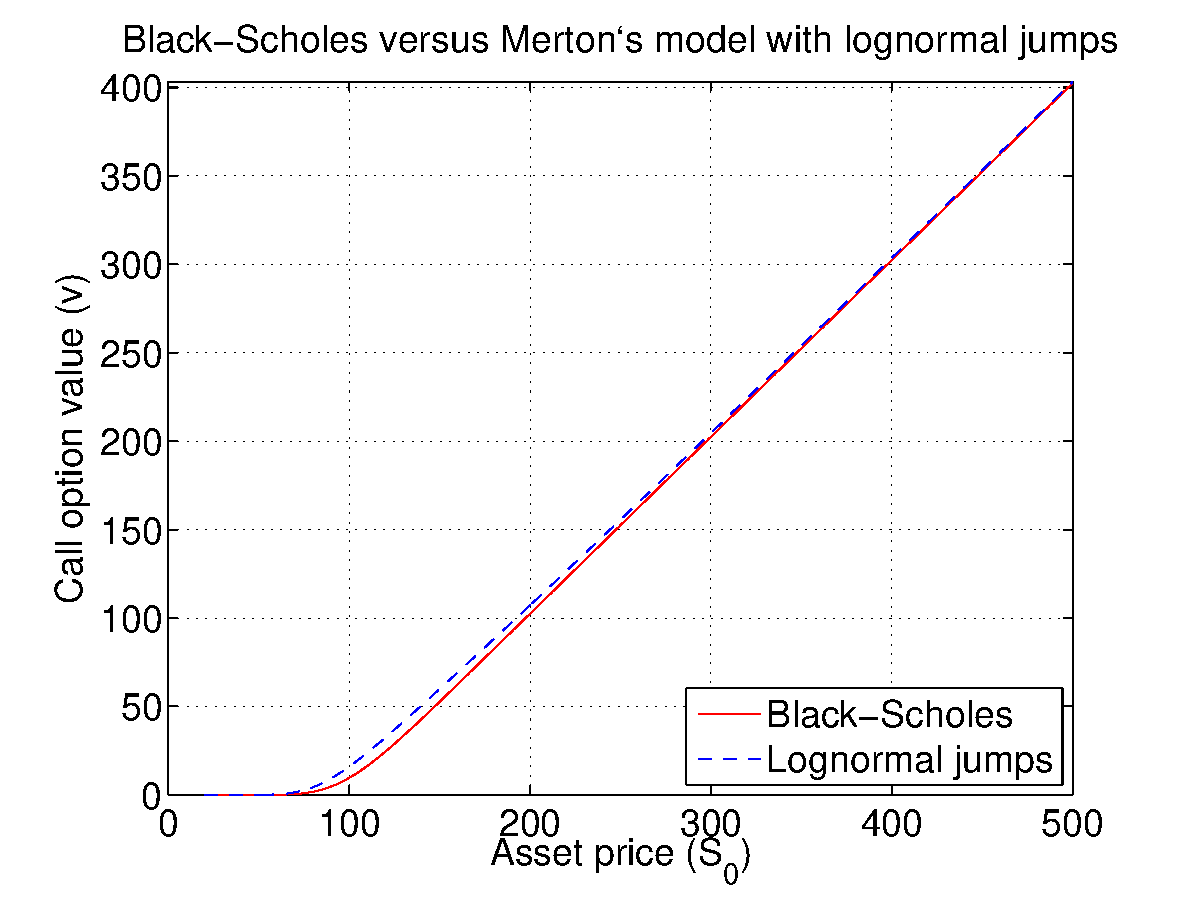
\includegraphics[width=0.6\linewidth]{figures/optionComp.eps}\hspace*{3pt}}
		\subfigure[Difference between \eqref{eqn:mertonSoln} and \eqref{eqn:EUcall}. \label{fig:optionDiff}]{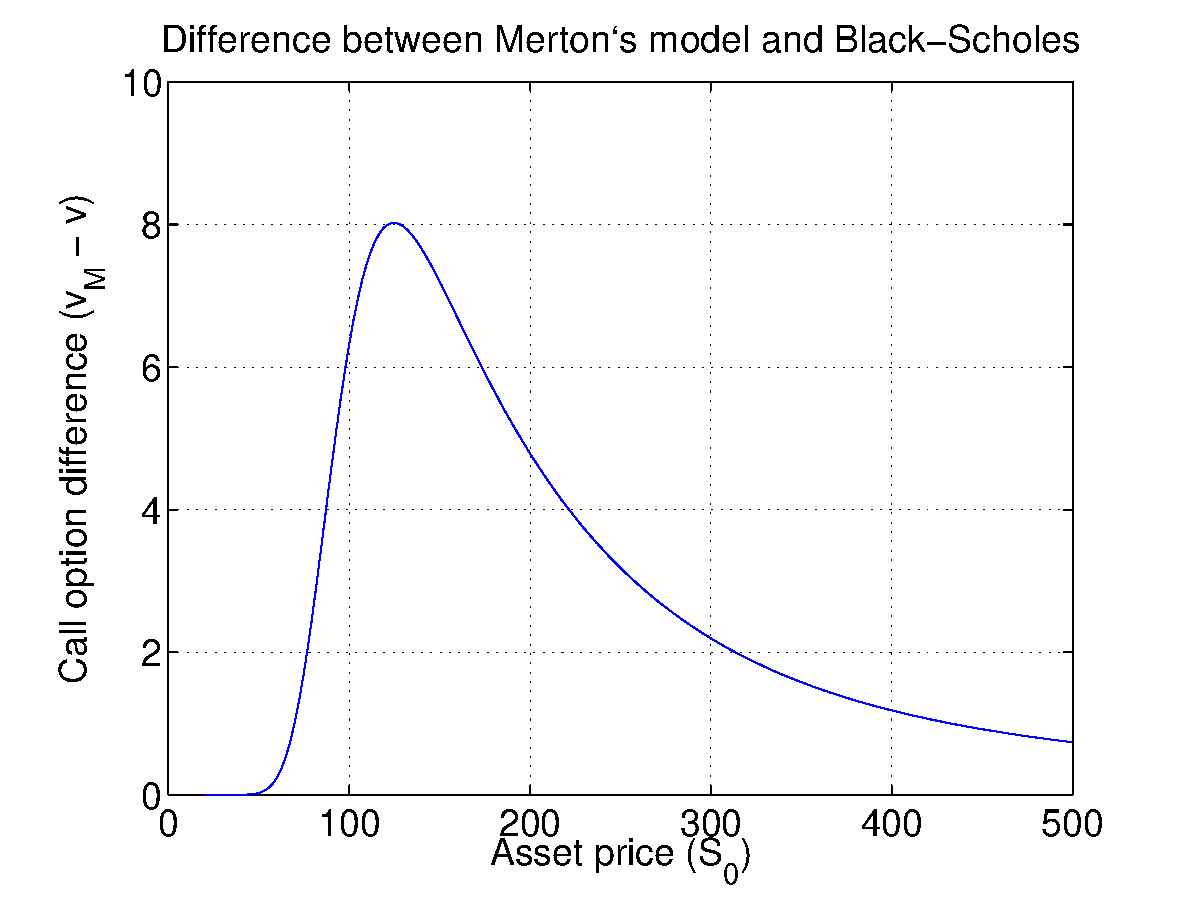
\includegraphics[width=0.6\linewidth]{figures/optionDiff.eps}
			}
		\caption{Call option profiles using \eqref{eqn:EUcall} and \eqref{eqn:mertonSoln}. The financial parameters are $r = 0.05$, $q=0.00$, $\sigma = 0.3$, $T-t = 0.5$, $K = 100$, and $S_0 \in [50,500]$. The lognormal jump parameters are $\lambda = 0.5$, $\mu_Y = -0.90$, and $\sigma_Y = 0.45$.}
		\label{fig:optionComp}
\end{figure}

\section{Example: double exponentially distributed jumps}
We will also demonstrate how to derive a recursive formula for double exponentially distributed jumps. A pricing formula does exist~\cite{Kou2002, Kou2004} for a double exponential jump-diffusion model, but it is expressed in a way that showing equality to the recursive form \eqref{eqn:Fn} is very difficult. Thus only $F_1$ will be determined since it is all that is required to generate the other terms.

Suppose $Y > 0$ is drawn from a double exponential distribution with parameters $\omega_1 > 0, \, \omega_2 > 0$, and $p, \, q \geq 0$ such that $p + q = 1$. Frontczak~\cite{Frontczak2013} gives the corresponding PDF and expectation as
	\begin{equation*}
		f(y) = p\omega_1y^{-\omega_1-1}\1_{\{y\geq 1\}} + q\omega_2y^{\omega_2-1}\1_{\{0 < y < 1\}}, \quad \E[Y^{-\xi}] = \fr{p\omega_1}{\omega_1+\xi} + \fr{q\omega_2}{\omega_2-\xi},
	\end{equation*}
where $\1_{I}$ is the indicator function of the interval $I$. Using \eqref{eqn:Fn}, we get
	\begin{align}
		\label{eqn:doubleExp}
		\begin{split}
		F_1(x) &= \fr{1}{x}\left( p\omega_1\left(\fr{1}{x} \right)^{-\omega_1-1}\1_{\left\{ 1/x \geq 1 \right\}} + q\omega_2\left( \fr{1}{x} \right)^{\omega_2-1}\1_{\left\{ 0 < 1/x < 1 \right\}} \right) \\
		&= p\omega_1x^{\omega_1}\1_{\{ x \leq 1 \}} + q\omega_2x^{-\omega_2}\1_{\{x > 1\}},
		\end{split}
	\end{align}
and from here we can obtain $F_n$ recursively from \eqref{eqn:Fn}. Using this, we can substitute into \eqref{eqn:jumpGeneral} and then \eqref{eqn:optionJump} to find the option price.


\section{Example: gamma distributed jumps}
Whilst a pricing formula for lognormal jumps and double exponential jumps have been derived previously, none exists for gamma distributed jumps. We will show a recursive solution that is still exact and analytic.

Suppose $Y \sim \text{Gamma}(\alpha_Y,\beta_Y)$, where $\alpha_Y > 0$ affects the distribution shape and $\beta_Y > 0$ determines the scale (i.e., how far spread out the distribution is). The associated PDF of $Y$ is given by~\cite{Frontczak2013}
	\begin{equation*}
		f(y) = \fr{1}{\Gamma(\alpha_Y)\beta_Y^{\alpha_Y}}y^{\alpha_Y-1}e^{-y/\beta_Y}, \qquad \E[Y^{-\xi}] = \fr{\beta_Y^{-\xi}\Gamma(\alpha_Y-\xi)}{\Gamma(\alpha_Y)}.
	\end{equation*}
Then using \eqref{eqn:jumpGeneral}, we have
	\begin{equation}
		\label{eqn:gammaJump}
		F_1(x) = \fr{1}{x}\fr{1}{\Gamma(\alpha_Y)\beta_Y^{\alpha_Y}}\left(\fr{1}{x}\right)^{\alpha_Y-1}e^{-1/(x\beta_Y)} = \fr{(x\beta_Y)^{-\alpha_Y}}{\Gamma(\alpha_Y)}e^{-1/(x\beta_Y)},
	\end{equation}
which can then be employed recursively to compute $F_n$. Similarly, $F_n$ can be substituted into \eqref{eqn:jumpGeneral} and then \eqref{eqn:optionJump} to find the corresponding option price.

%We will present two methods to derive the formula: 1) brute-force Mellin inversion but still bypassing direct complex integral computation, and 2) using \eqref{eqn:jumpGeneral} to determine the jump.

%\subsubsection{Brute-force Mellin inversion}
%In order to obtain an analytic pricing formula, we require $\J$. The key to determining $\J$ is to compute $\M^{-1}\left\{ \E[Y^{-\xi}]^n \right\}$. First, we have
%	\begin{equation*}
%		 \E[Y^{-\xi}]^n = \left( \fr{\beta^{-n\xi}}{\Gamma(\alpha)^n} \right)\Gamma(\alpha-\xi)^n.
%	\end{equation*}
%To calculate its inverse Mellin, we require the following lemmas:

%\begin{lemma}
%	\label{lem:2}
%	For some $\beta$, $n \in \mathbb{R}$, we have
%		\begin{equation*}
%			\M\left\{ \fr{\delta\left( x - \fr{1}{\beta^n} \right)}{\beta^n} \right\} = \beta^{-n\xi},
%		\end{equation*}
%	where $\delta$ is the standard Dirac delta function.
%\end{lemma}
%\begin{proof}
%	See Appendix \ref{subsec:lem2}.
%\end{proof}
%\begin{lemma}
%	\label{lem:3}
%	For some $\alpha \in \mathbb{R}$, we have
%		\begin{equation*}
%			\M\left\{ x^{-\alpha}e^{-1/x} \right\} = \Gamma(\alpha - \xi),
%		\end{equation*}
%	where $\Gamma$ is the standard gamma function.
%\end{lemma}
%\begin{proof}
%	See Appendix \ref{subsec:lem3}.
%\end{proof}
%Next, we let $G_n$ be a function such that $\M\left\{ G_n(x) \right\} = \Gamma(\alpha - \xi)^n$. We can rewrite this to be
%	\begin{align*}
%		\M\left\{ G_n(x) \right\} = \Gamma(\alpha - \xi)\Gamma(\alpha - \xi)^{n-1} = \M\left\{ G_1(x) \right\} \M\left\{ G_{n-1}(x) \right\},
%	\end{align*}
%and using the convolution property, we invert this to give
%	\begin{equation*}
%		G_n(x) = \int_0^\infty \fr{1}{z}G_1(z)G_{n-1}\left(\fr{x}{z}\right) \, \d z.
%	\end{equation*}
%Once again, we require a base case to make this recursive formula work. Computing $G_1$ is simple by applying lemma \ref{lem:3} to produce
%	\begin{align*}
%		G_1(x) = \M^{-1}\left\{ \Gamma(\alpha - \xi) \right\} = x^{-\alpha}e^{-1/x}.
%	\end{align*}


\section{Discussion and conclusion}
The key result presented in this chapter was the alternative pricing formula \eqref{eqn:optionJump} for options in a jump-diffusion model for the underlying asset. There are several advantages to this new formula. Firstly, \eqref{eqn:optionJump} is applicable to any general payoff and type of jump. Merton's formula is only applicable when the jump is drawn from a particular distribution, namely, the lognormal distribution. On the other hand, Frontczak's formula is also applicable to any general payoff and type of jump as in \eqref{eqn:optionJump}, but a complex integral has to be evaluated in Frontczak's result and reduces to \eqref{eqn:mertonSoln} for a given payoff and jump. However, the integrals in \eqref{eqn:optionJump} are all real since the Mellin transform inversion has been performed in a different manner to~\cite{Frontczak2013} where the inversion was completed via a complex integral.

Equation \eqref{eqn:optionJump} conveniently represents the standard European option value with shifted parameters and a function which mimics the discontinuous jumps. If multiple types of options are to be priced or if the jump dynamics were changed, \eqref{eqn:optionJump} is in a form whereby any alterations can be easily incorporated since the jump function is completely separated from any other component of the pricing formula. Additionally, the general pricing formula in \cite{Frontczak2013} is expressed as a complex integral with the jump dynamics embedded across multiple terms. In practice, this would be unfavourable as computing complex integrals is relatively expensive when compared to real integrals. %Furthermore, modifying any characteristics regarding the jump (e.g., the distribution) or the payoff would also be quite disadvantageous as it is unclear what terms would need to be amended.
%To complete the result, we also derived a general formula \eqref{eqn:jumpGeneral} which can be computed for any jump following any given distribution. One of the primary advantages of this scheme is the avoidance of complex integration and no ansatz approach is required. Sources like \cite{Frontczak2013} and \cite{Merton1976} often bulk the behaviour of the jump with other terms of financial significance. Whilst it may be economic in terms of notation, it often masks the process that is occurring in regards to the jump-diffusion dynamics within the asset and how that ultimately affects the option pricing process.

Examples were given for the cases where the jumps have distributions that are lognormal, double exponential, and gamma. For lognormal jumps, both \cite{Merton1976} and \cite{Frontczak2013} also derived similar results; Merton's classical formula~\eqref{eqn:mertonSoln} exploited the properties of expectations whilst Frontczak's formula computed the Mellin inverse via algebraic manipulation and the Mellin convolution. Equation~\eqref{eqn:optionLN} was derived using convolution and direct inversion that bypasses the complex integral evaluation employed by Frontczak. One approach used \eqref{eqn:jumpGeneral} to compute the terms recursively whilst the other relied on the properties of the exponential function which simplified the algebra tremendously. It should be emphasized that in \eqref{eqn:optionLN}, having the jump term isolated from the remainder of the formula is convenient since it allows for the pricing process to be modular. That is, one can calculate the necessary jump term before determining the option price at the specified parameter values. Not only is the separation preferable for computation, it reiterates the notion of interchangeability: if the jump dynamics were to change, \eqref{eqn:optionJump} together with \eqref{eqn:jumpGeneral} would be able to accommodate this efficiently. %Albeit complex inversion would produce the exact answer without the potential for a recursive formulation, finding this might be difficult.
Although \eqref{eqn:jumpGeneral} is recursive in the general case, one may obtain some insight into what $F_n$ is by carefully analysing the distribution of the jump. This could ultimately lead to easier calculations. Consequently, it is possible to derive pricing formulas for any types of jumps as shown with the double exponential distribution in \eqref{eqn:doubleExp} and the gamma distribution in \eqref{eqn:gammaJump}. The key is being able to calculate each term in the sequence $F_1, F_2, \ldots$. If the integrals associated with $F_n$ are too complicated to solve analytically, one may resort to numerics to yield approximate solutions to \eqref{eqn:jumpGeneral}. For the double exponential and gamma distributions, we kept the jump terms in a recursive form to demonstrate the capability of \eqref{eqn:jumpGeneral}. However, it is not clear how to obtain a non-recursive form for $F_n$ for double exponentially and gamma distributed jumps as we did for the lognormal jumps.

There is also interest in finding an exact solution for Kou's double exponentially distributed jumps \cite{Kou2002, Kou2004} using \eqref{eqn:optionJump} and \eqref{eqn:jumpGeneral} since \textcolor{blue}{recent empirical studies (in particular, the tests performed in~\cite{Ramezani1998}) suggest a better model for the asset process involves the jumps following a double exponential distribution.} In particular, it may be of interest to see whether or not a Mellin transform route would generate a more elegant and simple solution in lieu of Kou's original solution, which involves the computation of quite complicated $Hh$ functions (see \cite[pp. 691]{Abramowitz1972}). There is also the possibility to extend \eqref{eqn:optionJump} to price American options in jump-diffusion models, which will be examined in chapter 5 of this thesis.
	
In conclusion, we have devised and introduced a new scheme for option pricing when the asset follows jump-diffusion dynamics. In particular, we were able to formulate this new model to fit any type of jump. The consequent result can be computed recursively within an infinite sum. This was achieved by implementing the properties of the Mellin transform and the Black-Scholes kernel. We also highlighted how the recursion is handled when the jump is extracted from a lognormal distribution and also provided some insight into how the recursion can be computed when the jump is double exponentially and gamma distributed. 


   \chapter[Implied volatility estimation for European options in jump-diffusion dynamics]{Implied volatility estimation for European options in jump-diffusion dynamics}
\chaptermark{Implied volatility -- European options with jumps}

\section{A PIDE analogue of Dupire's equation}
In this section, we will derive a PIDE that is the analogue of Dupire's equation as seen in \cite{Gatheral2006}. The Dupire-like PIDE will serve as the platform for computing the implied volatility of options with jump-diffusion asset dynamics.

\subsection{Homogeneity of the solution}
First, we assume that the payoff function $\phi$ now depends on a parameter~$x' > 0$ (i.e., $\phi = \phi(x;x')$).  The motivation for this is that in the case of a European put or call, $x'$ represents the strike price. Furthermore, we assume that $\phi$ is homogeneous of degree one in~$x$ and $x'$. \textcolor{blue}{That is, we assume
$$
	\phi(\beta x; \beta x') = \beta \phi(x;x').
$$}
Note that standard put and call payoffs satisfy this assumption. We show that the option price function~$v$ is homogeneous of degree one in~$x$ and $x'$. That is, we want to show for $v = v(x,t; x')$ that
		\begin{equation}
			\label{eqn:homogen}
			v(\beta x, t; \beta x') = \beta v(x,t; x')
		\end{equation}
for all $\beta > 0$. This equality can be proven via a uniqueness argument as follows. We first express \eqref{eqn:PIDE} as $\mathscr{L} v = 0$. Now let $w = w(x,t; x')$ solve the following final value problem:
		\begin{align}
			\label{eqn:subPIDE}
			\begin{split}
			&\mathscr{L}w = 0, \qquad w(x,T; x') = \beta\phi(x;x').
			\end{split}
		\end{align}
Next, we define the function $v_1(x,t;x') = \beta v(x,t;x')$, where $v$ is a solution to (\ref{eqn:PIDE}), (\ref{eqn:PIDEcondition}). Then
	\begin{align*}
		\mathscr{L}v_1 = \beta \mathscr{L}v = 0.
	\end{align*}
For the terminal condition, since $v(x,T;x') = \phi(x;x')$, this implies that
	\begin{equation*}
		v_1(x,T;x') = \beta v(x,T; x') = \beta\phi(x;x').
	\end{equation*}
Therefore $v_1$ satisfies the final value problem \eqref{eqn:subPIDE}. On the other hand, we now let $v_2(x,t,x') = v(\beta x, t; \beta x')$. Computing the derivatives gives
	\begin{equation*}
		\fr{\pr v_2}{\pr x} = \beta D_1v, \quad \fr{\pr^2 v_2}{\pr x^2} = \beta^2 D_{11}v,
	\end{equation*}
where $D_1$ and $D_{11}$ represent the first and second partial derivatives with respect to the first argument, respectively. Substituting these into (\ref{eqn:subPIDE}), we get
	\begin{align*}
		\mathscr{L}v_2 = \mathscr{L}v = 0,
	\end{align*}
and by the homogeneity of $\phi$, the terminal condition is
	\begin{align*}
		v_2(x,T;x') = v\left( \beta x, T; \beta x' \right) = \phi(\beta x; \beta x') = \beta \phi(x;x').
	\end{align*}
Hence $v_2$ also satisfies the final value problem \eqref{eqn:subPIDE}. By uniqueness, we have
	\begin{equation*}
		v\left(\beta x, t; \beta x'\right) = v_2(x,t;x') = v_1(x,t;x') = \beta v(x,t;x'),
	\end{equation*}
thus proving the homogeneity property for $v$ and any general payoff $\phi$ that is homogeneous of degree one in~$x$ and $x'$.

\subsection{Derivation of a Dupire-like PIDE via Euler's theorem on homogeneous functions}
The partial derivatives of the Dupire equation~\cite{Gatheral2006} \textcolor{blue}{are with respect to the strike price $K$.} Thus to derive a Dupire-like PIDE, we will require partial derivatives in terms of $x'$ (the analogous variable for $K$). This can be done by invoking Euler's theorem for homogeneous functions~\cite[pp. 317]{Kishan2007} to $v$ and we get
	\begin{equation*}
		x\fr{\pr v}{\pr x} + x'\fr{\pr v}{\pr x'} = v,
	\end{equation*}
since $v$ has been shown to be homogeneous in $x$ and $x'$ of degree one. By differentiating the above equation with respect to $x$ and $x'$, we obtain
	\begin{equation*}
		x\fr{\pr^2 v}{\pr x^2} = -x'\fr{\pr^2 v}{\pr x \pr x'}, \quad x'\fr{\pr^2 v}{\pr x'^2} = -x\fr{\pr^2 v}{\pr x' \pr x},
	\end{equation*}
respectively. Hence it follows that
	\begin{equation*}
		x^2\fr{\pr^2 v}{\pr x^2} = x'^2\fr{\pr^2 v}{\pr x'^2}.
	\end{equation*}
The only term left to account for is the integral in (\ref{eqn:PIDE}). Notice that the first integrand term depends on~$y$; we want to transfer the dependency on $y$ to the third argument (i.e., $x'$). This can be achieved by the homogeneity property in (\ref{eqn:homogen}), and we obtain
	\begin{align*}
		v(xy,t; x') &= v\left(xy,t;\fr{x'y}{y}\right) = yv\left( x,t;\fr{x'}{y} \right).
	\end{align*}
Thus, setting $u(x',t; x) = v(x,t; x')$ and replacing all the $x$ derivatives with $x'$ derivatives and substituting the above rearrangement for the integrand, we get
	\begin{align}
		\label{eqn:DupireLike}
		\begin{split}
		\fr{\pr u}{\pr t} &- (q(t) + \kappa\lambda)u - (r(t) - q(t) - \kappa\lambda)x'\fr{\pr u}{\pr x'} + \fr{1}{2}\sigma(t)^2x'^2\fr{\pr^2 u}{\pr x'^2} \\
		& {} + \lambda \int_0^\infty \left( yu\left( \fr{x'}{y},t; x \right) - u(x',t; x) \right)f(y) \, \d y = 0
		\end{split}
	\end{align}
with
	\begin{equation}
		\label{eqn:DupireCond}
		u(x',T; x) = \phi(x';x),
	\end{equation}
since $u$ now depends on the variables $x'$ and $t$ with $x$ as a parameter. Equations~(\ref{eqn:DupireLike}) and (\ref{eqn:DupireCond}) together form the Dupire-like PIDE system for options in a jump-diffusion framework. Note that this reduces to the standard Dupire PDE as seen in \cite{Gatheral2006} in the absence of jumps (i.e., $\lambda = 0$) when $\phi$ is either the call or put payoff.

\section{Implied volatility formula}
From (\ref{eqn:DupireLike}) and (\ref{eqn:DupireCond}), it is possible to now solve the inverse problem of implied volatility estimation. Throughout the remainder of this section, we will assume that~$r$ and $q$ are constants. Suppose that we are given $u(x',0;S_0)$ for all $x' > 0$. We wish to derive an explicit formula for $\sigma$ in terms of certain integrals of $u$ with respect to $x'$. The reason for this is that in practice one can observe different time-zero option prices~$u_1,\, u_2, \, \ldots, u_m$ for varying strike prices~$K_1, \, K_2, \, \ldots, K_m$, here corresponding to different values of $x'$. Once we can extrapolate $u$ for extreme values of $x'$, we would know the entire time-zero profile of $u$.

First, denote by $\hat u$ the Mellin transform of $u$ with respect to $x'$, i.e.,
	\begin{equation*}
		\hat u(\xi,t) = \int_0^\infty (x')^{\xi-1} u(x',t; x) \, \d x'.
	\end{equation*}
We take the Mellin transform of (\ref{eqn:DupireLike}) and (\ref{eqn:DupireCond}) with respect to $x'$ to obtain
	\begin{align}
		\label{eqn:mellinDUPIRE}
		\begin{split}
			\fr{\pr \hat u}{\pr t} - G_{\lambda}(\xi)\hat u(\xi,t) = 0, \quad \hat u(\xi,T) = \hat \phi(\xi),
		\end{split}
	\end{align}
where
	\begin{equation}
		G_{\lambda}(\xi) = -\left( \fr{\sigma^2}{2}\xi(\xi+1) + (r - q - \kappa\lambda)\xi - (	q + \kappa\lambda) + \lambda\E[Y^{\xi+1} - 1] \right).
	\end{equation}
We are left with an ODE in $t$. Solving (\ref{eqn:mellinDUPIRE}) gives
	\begin{equation}
		\label{eqn:mellinDUPIREode}
		\hat u(\xi,t) = e^{-G_{\lambda}(\xi)(T-t)}\hat \phi(\xi).
	\end{equation}
We can proceed to isolate $\sigma^2$ in (\ref{eqn:mellinDUPIREode}) to yield
	\begin{align}
		\label{eqn:sigmaMellin}
		\begin{split}
		\sigma^2 &= \fr{2}{\xi(\xi+1)}\bigg( \fr{\ln( \hat u(\xi,t)/\hat\phi(\xi) )}{T-t} - (r-q-\kappa\lambda)\xi + (q+\kappa\lambda) - \lambda\E[Y^{\xi+1} - 1] \bigg),
		\end{split}
	\end{align}
where we have the flexibility to choose a value of $\xi$. Theoretically, $\sigma^2$ should be constant for any value of $\xi$ and $t$, provided the Mellin transform of $u$ exists. Furthermore, it should be emphasised that (\ref{eqn:sigmaMellin}) can be applied to any type of payoff and jump. When $\lambda = 0$, \eqref{eqn:sigmaMellin} gives an explicit formula for the implied volatility in the usual diffusion framework.

\section{Numerical simulations}
\label{sec:numerics}
This section will contain the numerical results obtained from the implied volatility formula (\ref{eqn:sigmaMellin}) for lognormal jumps. To test the validity of the model, we will require an initial $\sigma$ value to generate option prices before solving the inverse problem. The results will be divided into two sets: the first set will be implementing purely theoretical data; the second set will be generated using pseudo-market data that attempts to mimic observed market prices and values. We will now elaborate on how the option prices are obtained. For definiteness, we will consider a time-zero European call where the underlying follows standard diffusion dynamics (i.e., no jumps). That is, in \eqref{eqn:EUcall} we set $t = 0$, $x = S_0$, assume $r$, $q$, and $\sigma$ are constant, and view this as a function of $K$ given as
	\begin{equation}
		\label{eqn:EUcallK}
		v^{\text{call}}(K) = S_0e^{-qT}N\left( z_1\left( \fr{S_0}{K}, 0, T \right) \right) - Ke^{-rT}N\left( z_2\left( \fr{S_0}{K}, 0, T \right) \right),
	\end{equation}
where $z_1$ and $z_2$ are defined as they are in \eqref{eqn:z1} and \eqref{eqn:z2}, respectively.

\subsection{Theoretical data for option prices}
The Mellin transform is valid in the domain $[0,\infty)$. Since this implied volatility scheme incorporates a Mellin transform with respect to the strike price~$K = x'$ for a fixed~$x = S_0$, we require time-zero option prices for varying $K \in [0,\infty)$. Numerically, we will use discrete 200 values of $K \in [1.0\times10^{-6},8S_0]$ evenly spaced to simulate continuity for the entire domain $K > 0$. This will yield 200 call prices.  In practice, this is seldom applicable as many sources for financial data will only list discrete option prices for a finite set of $K$ values (i.e., much less than 200) and for a fixed asset price~$S_0$. Furthermore, it is often implausible to expect the domain of $K$ to be uniformly spaced. This approach is only included to illustrate the accuracy of the model assuming a very smooth dataset.

\subsection{Pseudo-market data for option prices}
As mentioned before, the finite number of discrete option prices may prove insufficient in exhibiting a continuous behaviour in the option price profile. Hence we require a method for approximating the data beyond the option prices provided. The following procedure will be demonstrated for a call option in the absence of jumps to simplify the calculations. However, these steps can be adapted when accounting for jumps in the asset dynamics.

We assume that we have a set of call prices~$v_1 > v_2 > \cdots > v_{m - 1} > v_m$ with corresponding strike prices~$K_1 < K_2 < \cdots < K_{m - 1} < K_m$. It is known from \cite{Bowling2009} that the best one-parameter logistic approximation of the standard normal CDF $N$ for all $z \in \R$ is given by
	\begin{equation*}
		N(z) \approx \frac{1}{1 + e^{-a z}}, \quad a = 1.702,
	\end{equation*}
where the maximum difference between the approximation and exact expression for $N$ is less than $0.001$ for $z \in [-4.5,4.5]$. %Check what happens outside -4.5 and 4.5
Now for $z < 0$ we have
	\begin{equation*}
		N(z) \approx \fr{e^{az}}{1+e^{az}} = e^{az}(1-e^{az}+e^{2az}-\cdots) = e^{az} - e^{2az} + e^{3az} - \cdots.
	\end{equation*}
Hence we can take $N(z) \approx e^{az}$ for $z \ll -1$. Using this logistic estimation in \eqref{eqn:EUcallK}, this approximates to
	\begin{equation*}
		v^{\text{call}}(K) \approx \frac{S_0 e^{-q T}}{1 + e^{-a d_1(S_0/K,0,T)}} - \frac{K e^{-r T}}{1 + e^		{-a d_2(S_0/K,0,T)}} = \frac{S_0 e^{-q T}}{1 + e^{-a d_1}} - \frac{K e^{-r T}}{1 + e^		{-a d_2}},
	\end{equation*}
where $d_1$ and $d_2$ are defined as
	\begin{equation*}
		d_1 = z_1\left( \fr{S_0}{K},0,T \right), \quad d_2 = z_2\left( \fr{S_0}{K}, 0, T\right)
	\end{equation*}
using \eqref{eqn:z1} and \eqref{eqn:z2}, respectively under the assumption of constant parameters.
When $|K| \ll 1$ we see that $d_1 \gg 1$ and $d_2 \gg 1$; hence $v^{\text{call}}(K) \approx S_0 e^{-q T} - K e^{-r T}$. Therefore we assume that
	\begin{equation*}
		v^{\text{call}}(K) = S_0e^{-qT} - \beta K, \quad 0 < K \le K_1
	\end{equation*}
for some $\beta > 0$. Using $K_1$ to extrapolate, we see from $v^{\text{call}}(K_1) = v_1$ that we obtain
%Therefore we assume that
%\begin{equation*}
%\Vcall(K) = \kappa - \beta K, \quad 0 < K \le K_2
%\end{equation*}
%for some $\kappa, \beta > 0$. From $\Vcall(K_1) = V_1$ and $\Vcall(K_2) = V_2$ we obtain
	\begin{equation*}
		\beta = \fr{S_0e^{-qT} - v_1}{K_1}.
	\end{equation*}
Conversely, when $K \gg 0$ we have $-d_1 \gg 1$ and $-d_2 \gg 1$. Using $N(z) \approx e^{az}$ for $-z \gg 1$, we can simplify $N(d_1)$ and $N(d_2)$ and approximate \eqref{eqn:EUcallK} by
	\begin{equation*}
		v^{\text{call}}(K) \approx S_0 e^{-q T} e^{a d_1} - K e^{-r T} e^{a d_2}.
	\end{equation*}
As $d_1 = d_2 + \sigma \sqrt{T}$,
	\begin{equation*}
		e^{a d_2} = e^{a\left(\log(S_0/K) + (r - q - \sigma^2/2) T\right)/\left(\sigma \sqrt{T}\right)} = \left(\frac{S_0}{K}\right)^{a/\left(\sigma \sqrt{T}\right)} e^{a(r - q - \sigma^2/2) \sqrt{T}/\sigma}.
	\end{equation*}
Similarly,
	\begin{equation*}
		e^{a d_1} = e^{a \sigma \sqrt{T}} e^{a d_2},
	\end{equation*}
hence we have
	\begin{equation*}
		v^{\text{call}}(K) \approx \left(S_0 e^{-q T} e^{a \sigma \sqrt{T}} - K e^{-r T}\right) \left(\frac			{S_0}{K}\right)^{a/\left(\sigma \sqrt{T}\right)} e^{a (r - q - \sigma^2/2) \sqrt{T}/\sigma}.
	\end{equation*}
Therefore we assume that
	\begin{equation*}
		v^{\text{call}}(K) = \frac{\gamma_1}{K^\delta} + \frac{\gamma_2}{K^{\delta-1}}, \quad K \ge K_{m}
	\end{equation*}
for some $\gamma_1,\gamma_2, \delta > 0$. We will need to use $K_{m-1}$ and $K_{m}$ to extrapolate, but we also require another data point. For the call option, $v^{\text{call}}(K) \rightarrow 0$ as $K \rightarrow \infty$, thus we let $K_L \gg K_m$ represent the strike price ``near'' infinity. We see from $v^{\text{call}}(K_{m - 1}) = v_{m - 1}$, $v^{\text{call}}(K_m) = v_m$, and $v^{\text{call}}(K_L) \approx 0$, and we deduce that
	\begin{align*}
		&\delta = \fr{\log\left( v_{m-1}/v_m\right) + \log\left((K_L - K_m)/(K_L-K_{m-1}) \right)}{\log(K_{m}/K_{m-1})}, \\
		&\gamma_2 = \frac{v_mK_m^\delta}{K_m - K_L}, \quad
		\gamma_1 = -K_L \gamma_2, \quad K_L \gg K_m.
	\end{align*}
Thus the call option function can be reformulated to become
	\begin{equation}
		\label{call-interpolate}
		v^\text{call}(K) =
			\begin{cases}
				S_0e^{-qT} - \beta K & 0 < K \le K_1,\\
				v_j & K = K_j, \enskip j = 1,\ldots,m,\\
				\frac{\gamma_1}{K^\delta} + \frac{\gamma_2}{K^{\delta-1}} & K \ge K_{m},
			\end{cases}
	\end{equation}
where $v_1,\ldots,v_m$ are the observed call prices. A similar process can also be adopted for the European call or put with jumps. Figures~\ref{fig:euro-call-bs} and~\ref{fig:euro-call-extrapolate} show the profile for the call option with both theoretical and pseudo-market data, respectively.

\begin{figure}[!h]
		\centering
		\subfigure[Call prices computed using \eqref{eqn:EUcallK} with $200$ equally spaced nodes for $K$ between $10^{-6}$ and $8S_0$. \label{fig:euro-call-bs}]{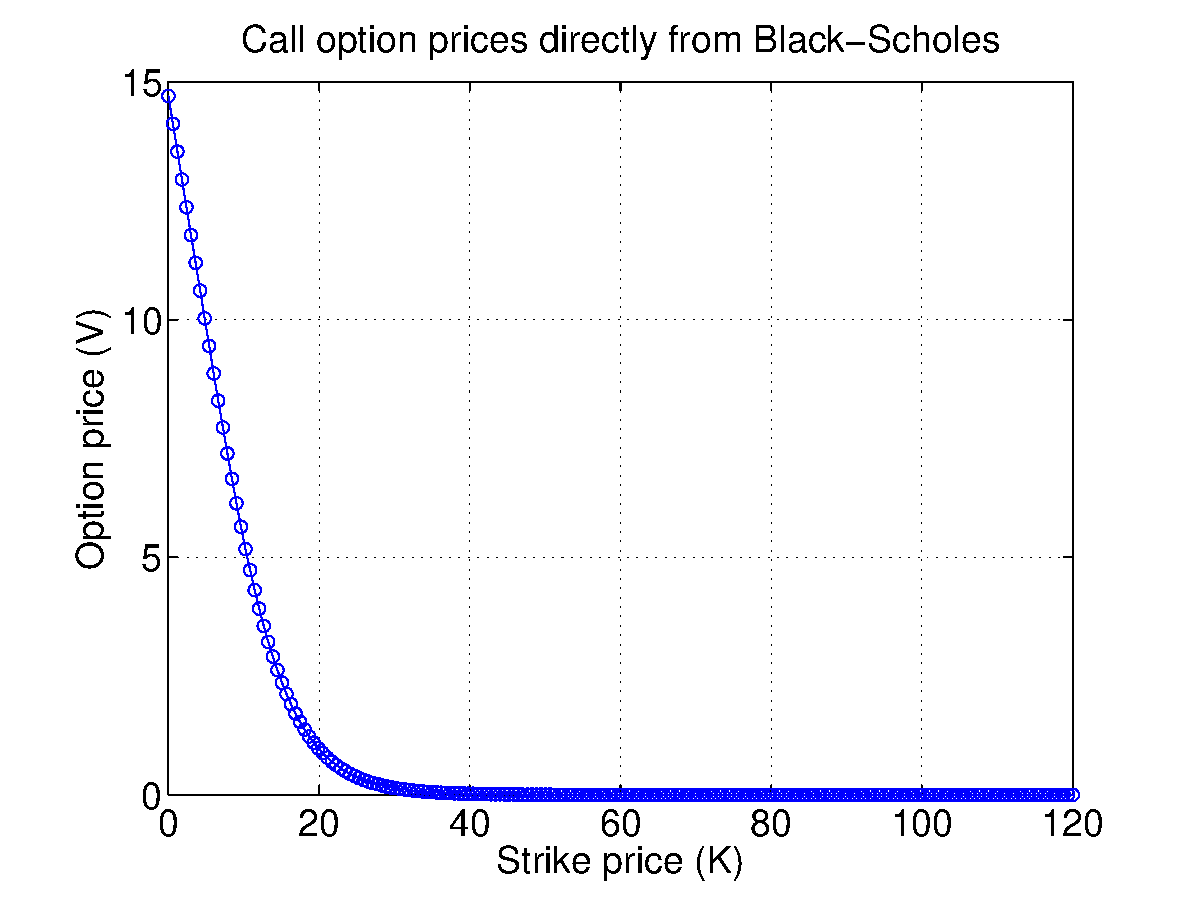
\includegraphics[width=0.49\linewidth]{figures/call-bs-prices.eps}\hspace*{3pt}}
		\subfigure[Call prices computed using \eqref{eqn:EUcallK} for pseudo-observed Black-Scholes values and \eqref{call-interpolate} to extrapolate. \label{fig:euro-call-extrapolate}]{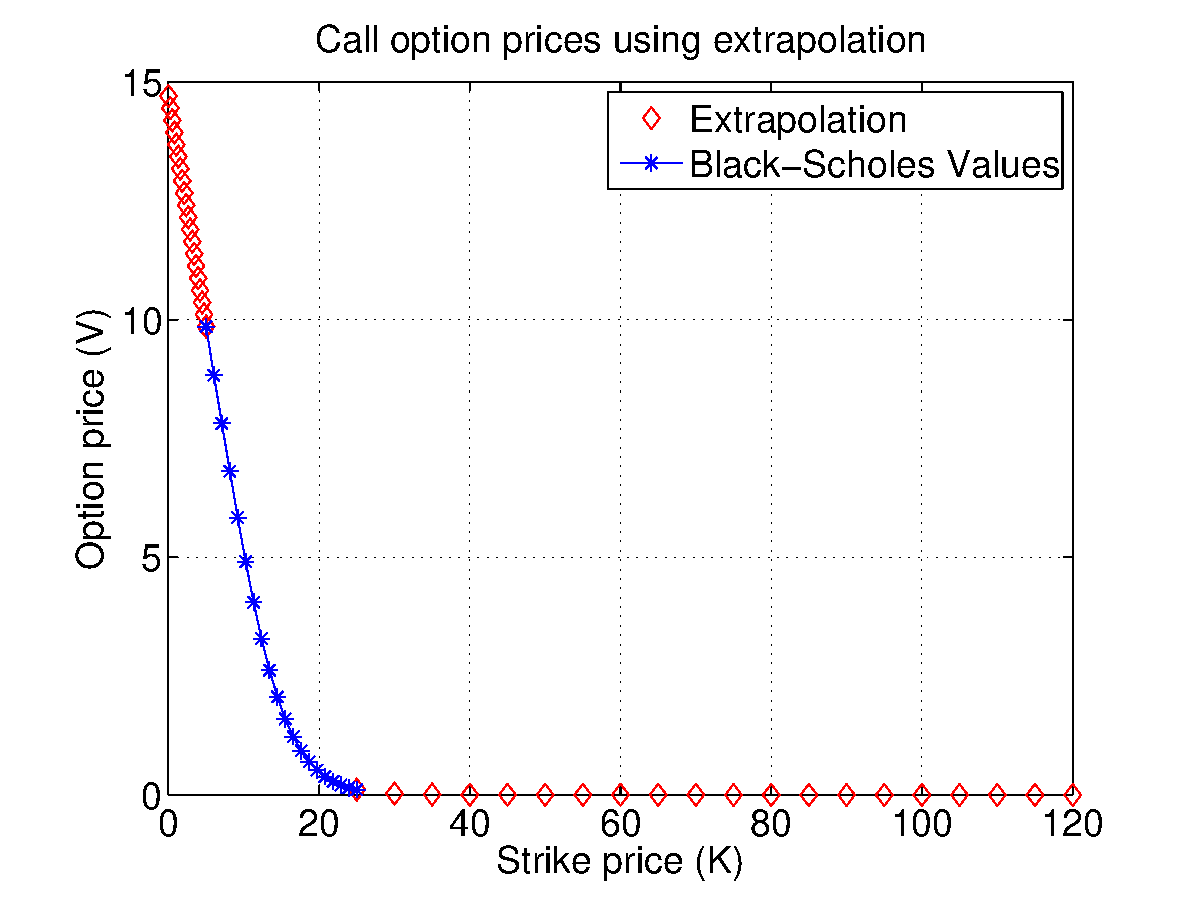
\includegraphics[width=0.49\linewidth]{figures/call-extrapolate-prices.eps}
			}
		\caption{Call option profiles for $K > 0$. The parameter values are $S_0 = 15$, $T = 0.3$, $r = 0.03$, $q=0.02$, and $\sigma = 0.3$.}
\end{figure}


\subsection{Algorithm}
The algorithm for computing $\sigma^2$ for a call option is as follows:
	\begin{enumerate}
		\item Obtain option data~$v_1, v_2,  \cdots,  v_m$~ for ~$K_1 < K_2 < \cdots < K_m$ either using theoretical, pseudo-market or actual market data.
			\begin{enumerate}
				\item Theoretical data -- use (\ref{eqn:EUcallK}) or (\ref{eqn:mertonSoln}) (with appropriate adjustments to the notation) and ensure ~$K_1, K_2, \hdots, K_m$ are 200 evenly spaced nodes between $10^{-6}$ and $8S_0$ (adjust if $8S_0 < K_m$).
				\item Pseudo-real or market data -- generate $v_1, v_2, \cdots, v_m$ using theoretical data or observed from the market, then use \eqref{call-interpolate} (adapt for jumps if necessary) to create more data points for a smoother profile. For $K \approx 0$, use $1.0\times10^{-6}$; for $K \gg 0$, use $8S_0$ (adjust if $8S_0 < K_m$).
			\end{enumerate}
		\item Choose a value of $\xi$.
		\item Evaluate $\hat v^\text{call}(\xi) = \int_0^\infty K^{\xi - 1} v^\text{call}(K) \, \d K$ via numerical integration (e.g., Gauss-Lobatto or Gauss-Kronrod quadrature), where $v^\text{call}$ is the entire time-zero option profile.
		\item Substitute the value for $\hat v^\text{call}(\xi)$ into \eqref{eqn:sigmaMellin} and compute $\sigma^2$.
	\end{enumerate}


\subsection{Results}

We will now report the implied volatility estimations for both theoretical option data and pseudo-market option prices via extrapolation. The parameter values used are $S_0 = 15$, $r = 0.05$, $q = 0.03$, and $T = 0.025$. We used $\sigma = 0.15$ and $\sigma = 0.3$ as initial seeds to generate the corresponding option prices. All simulations are performed in MATLAB using a European call option (with and without jumps). The Mellin transform is computed using the adaptive Gauss-Kronrod quadrature scheme available in MATLAB. The MATLAB code is provided in Appendix C.2.

\subsubsection{Theoretical data}
For the theoretical data, \eqref{eqn:optionLN} is used to generate 200 European call option prices with lognormal jumps for $K \in [1.0\times 10^{-6}, 8S_0]$. The associated lognormal parameters are chosen to be $\lambda = 0.10$, $\mu_Y = -0.90$, and $\sigma_Y = 0.45$. We generated 30 terms from the infinite series. To illustrate the consistency of the algorithm, several $\xi$ values are selected for the Mellin transform. The domain chosen is $\xi \in [1.0,5.0]$ in discrete increments of 0.25.
Tables~\ref{tab:sig015Theo} and \ref{tab:sig030Theo} show the numerical approximations for $\sigma$ against the true values.

\begin{table}\small{
\parbox{.45\linewidth}{
\centering
\begin{tabular}{ |c|c|c| }
\hline
\multicolumn{3}{ |c| }{\textbf{Implied volatility estimation for $\sigma = 0.15$}} \\
\multicolumn{3}{ |c| }{Avg. CPU time: 0.1 s}\\
\hline
$\xi$ & Estimated $\sigma$ & Absolute error \\ \hline
1.0 & 0.150001657453424 & $1.6 \times 10^{-6}$ \\
1.25 & 0.149999916945745 & $8.3 \times 10^{-8}$ \\
1.5 & 0.150004007140589 & $4.0 \times 10^{-6}$ \\
1.75 & 0.150000231848765 & $ 2.3 \times 10^{-7}$ \\
2.0 & 0.150000372512579 & $3.7 \times 10^{-7}$ \\
2.25 & 0.150000519892163 & $5.1 \times 10^{-7} $ \\
2.5 & 0.150000665164591& $6.6 \times 10^{-7}$ \\
2.75 & 0.150000808303685 & $ 8.0 \times 10^{-7} $ \\
3.0 & 0.150000949189142 & $ 9.4 \times 10^{-7} $ \\
3.25 & 0.150001087644665 & $1.0 \times 10^{-6}$ \\
3.5 & 0.150001223391692 & $ 1.2 \times 10^{-6} $ \\
3.75 & 0.150001355979046 & $ 1.3 \times 10^{-6}$ \\
4.0 & 0.150001484661131 & $ 1.4 \times 10^{-6}$ \\
4.25 & 0.150001608185628 & $1.6 \times 10^{-6}$ \\
4.5 & 0.150001724425047 & $ 1.7 \times 10^{-6}$ \\
4.75 & 0.150001829737164 & $1.8 \times 10^{-6}$ \\
5.0 & 0.150001917853050 & $1.9 \times 10^{-6}$ \\
\hline
\end{tabular}
\caption{Implied volatility estimations and errors for different $\xi$ when $\sigma = 0.15$ using pure theoretical option data from \eqref{eqn:optionLN}. Average CPU time is given in seconds.}
\label{tab:sig015Theo}
}
\hfill
\parbox{.45\linewidth}{
\centering
\begin{tabular}{ |c|c|c| }
\hline
\multicolumn{3}{ |c| }{\textbf{Implied volatility estimation for $\sigma = 0.3$}} \\
\multicolumn{3}{ |c| }{Avg. CPU time: 0.1 s}\\
\hline
$\xi$ & Estimated $\sigma$ & Absolute error \\ \hline
1.0 & 0.300000812537166 & $8.1 \times 10^{-7}$ \\
1.25 & 0.300000602264498 & $6.0 \times 10^{-7}$ \\
1.5 & 0.300001642090901 & $1.6 \times 10^{-6}$ \\
1.75 & 0.300000647148822 & $ 6.4 \times 10^{-7}$ \\
2.0 & 0.300000660419985 & $6.6 \times 10^{-7}$ \\
2.25 & 0.300000671406796 & $6.7 \times 10^{-7} $ \\
2.5 & 0.300000680367558 & $6.8 \times 10^{-7}$ \\
2.75 & 0.300000687348957 & $ 6.8 \times 10^{-7} $ \\
3.0 & 0.300000692310426 & $ 6.9 \times 10^{-7} $ \\
3.25 & 0.300000695116983 & $6.9 \times 10^{-7}$ \\
3.5 & 0.300000695475283 & $ 6.9 \times 10^{-7} $ \\
3.75 & 0.300000692830239 & $ 6.9 \times 10^{-7}$ \\
4.0 & 0.300000686190937 & $ 6.8 \times 10^{-7}$ \\
4.25 & 0.300000329275066 & $3.2 \times 10^{-7}$ \\
4.5 & 0.300000337379160 & $ 3.3 \times 10^{-7}$ \\
4.75 & 0.300000329776874 & $3.2 \times 10^{-7}$ \\
5.0 & 0.300000298131713 & $2.9 \times 10^{-7}$ \\
\hline
\end{tabular}
\caption{Implied volatility estimations and errors for different $\xi$ when $\sigma = 0.3$ using pure theoretical option data from \eqref{eqn:optionLN}. Average CPU time is given in seconds.}
\label{tab:sig030Theo}
}}
\end{table}

\begin{table}\small
\parbox{.45\linewidth}{
\centering
\begin{tabular}{ |c|c|c| }
\hline
\multicolumn{3}{ |c| }{\textbf{Implied volatility estimation for $\sigma = 0.15$}} \\
\multicolumn{3}{ |c| }{Avg. CPU time: 0.002 s}\\
\hline
$\xi$ & Estimated $\sigma$ & Absolute error \\ \hline
1.0 & 0.149998728439811 & $1.2 \times 10^{-6}$ \\
1.25 & 0.150027834813882 & $2.7 \times 10^{-5}$ \\
1.5 & 0.150054557535829 & $5.4 \times 10^{-5}$ \\
1.75 & 0.150080609531067 & $ 8.0 \times 10^{-5}$ \\
2.0 & 0.150106032110318 & $1.0 \times 10^{-4}$ \\
2.25 & 0.150130843920878 & $1.3 \times 10^{-4} $ \\
2.5 & 0.150155063080464 & $1.5 \times 10^{-4}$ \\
2.75 & 0.150178294968951 & $ 1.7 \times 10^{-4} $ \\
3.0 & 0.150201382384214 & $ 2.0 \times 10^{-4} $ \\
3.25 & 0.150223926634414 & $2.2 \times 10^{-4}$ \\
3.5 & 0.150245946705591 & $ 2.4 \times 10^{-4} $ \\
3.75 & 0.150267456617342 & $ 2.6 \times 10^{-4}$ \\
4.0 & 0.150288471381866 & $ 2.8 \times 10^{-4}$ \\
4.25 & 0.150309005551112 & $3.0 \times 10^{-4}$ \\
4.5 & 0.150329021452815 & $ 3.2 \times 10^{-4}$ \\
4.75 & 0.150348633294877 & $3.4 \times 10^{-4}$ \\
5.0 & 0.150367805351298 & $3.6 \times 10^{-4}$ \\
\hline
\end{tabular}
\caption{Implied volatility estimations and errors for different $\xi$ when $\sigma = 0.15$ using \eqref{eqn:EUcallK} to generate pseudo-market data. Average CPU time is given in seconds.}
\label{tab:sig015Pseudo}
}
\hfill
\parbox{.45\linewidth}{
\centering
\begin{tabular}{ |c|c|c| }
\hline
\multicolumn{3}{ |c| }{\textbf{Implied volatility estimation for $\sigma = 0.3$}} \\
\multicolumn{3}{ |c| }{Avg. CPU time: 0.002 s}\\
\hline
$\xi$ & Estimated $\sigma$ & Absolute error \\ \hline
1.0 & 0.300031895572929 & $3.1 \times 10^{-5}$ \\
1.25 & 0.300045257605552 & $4.5 \times 10^{-5}$ \\
1.5 & 0.300058090390309 & $5.8 \times 10^{-5}$ \\
1.75 & 0.300071242016552 & $ 7.1 \times 10^{-5}$ \\
2.0 & 0.300085040710682 & $8.5 \times 10^{-5}$ \\
2.25 & 0.300099577530501 & $9.9 \times 10^{-5} $ \\
2.5 & 0.300115017586394 & $1.1 \times 10^{-4}$ \\
2.75 & 0.300131558128381 & $ 1.3 \times 10^{-4} $ \\
3.0 & 0.300149410201347& $ 1.4 \times 10^{-4} $ \\
3.25 & 0.300168805884818 & $1.6 \times 10^{-4}$ \\
3.5 & 0.300190000681277 & $ 1.9 \times 10^{-4} $ \\
3.75 & 0.300213193710094 & $ 2.1 \times 10^{-4}$ \\
4.0 & 0.300238860932383 & $ 2.3 \times 10^{-4}$ \\
4.25 &0.300267261118478 & $2.6 \times 10^{-4}$ \\
4.5 & 0.300298771264214 & $ 2.9 \times 10^{-4}$ \\
4.75 & 0.300333806724048 & $3.3 \times 10^{-4}$ \\
5.0 & 0.300372824834949 & $3.7 \times 10^{-4}$ \\
\hline
\end{tabular}
\caption{Implied volatility estimations and errors for different $\xi$ when $\sigma = 0.3$ using \eqref{eqn:EUcallK} to generate pseudo-market data. Average CPU time is given in seconds.}
\label{tab:sig030Pseudo}

}
\end{table}

For the theoretical option prices, the implied volatility estimations for $\sigma = 0.15$ and $\sigma = 0.3$ prove to be quite accurate with errors in the order of $10^{-7}$ to $10^{-6}$. The error remains relatively consistent for all $\xi$ in the allocated domain, which further highlights the precision of the algorithm. It can be argued for $\sigma = 0.15$ that the absolute error is increasing as $\xi$ increases; however, this is primarily linked to approximation errors since the Mellin transform is computed numerically.

\subsubsection{Pseudo-market data}
The pseudo-market option prices are computed using \eqref{eqn:EUcallK} with 20 discrete values of $K \in [5,25]$, and then incorporates \eqref{call-interpolate} to extrapolate and provide continuity to the data.  Although we are considering a scenario with no jumps (i.e., $\lambda = 0$), a similar procedure may be applied in the case of jumps as seen in the previous section using pure theoretical data. Note that the discrete domain for $K$ will need to be adjusted accordingly if $S_0$ changes. Tables \ref{tab:sig015Pseudo} and \ref{tab:sig030Pseudo} list the results for the implied volatility estimation.

Once again, the results are quite satisfactory but the overall absolute error has increased in order of magnitude in comparison to the estimations yielded by the purely theoretical dataset. This is mainly attributed to the extrapolating functions in \eqref{call-interpolate}. Whilst it maintains the monotonicity of the option profile versus the strike price (e.g., monotonically decreasing for a European call against strike), the main source of error lies within the ``tail'' function (i.e., the approximation for the option price as $K \rightarrow \infty$). This will be elaborated upon in the discussion.

\subsubsection{Comparison to other methods}
We will now give a comparison of \eqref{eqn:sigmaMellin} against two other formulas for implied volatility estimation. \textcolor{black}{We first denote $v^\text{call}$ to be observed European call price that is required to compute the implied volatility}. We will use the result by Brenner and Subrahmanyam~\cite{Brenner1988}
	\begin{equation}
		\label{eqn:brensub}
		\sigma \approx \fr{v^\text{call}}{S_0}\sqrt{\fr{2\pi}{T}},
	\end{equation}
Corrado and Miller~\cite{Corrado1996}
	\begin{equation}
		\label{eqn:corrado}
		\sigma \approx \fr{1}{S_0 + K}\sqrt{\fr{2\pi}{T}}\left( v^\text{call} - \fr{S_0 - K}{2} + \sqrt{\left( v^\text{call} - \fr{(S_0 - K)}{2} \right)^2 - \fr{(S_0-K)^2}{\pi} } \right),
	\end{equation}
\textcolor{black}{and a standard Newton's method approach~\cite{Higham2004}
    \begin{equation}
        \label{eqn:newton}
        \sigma_{n+1} = \sigma_n - \fr{F(\sigma_n)}{F'(\sigma_n)},
    \end{equation}
where $F$ is the difference between value of the European call~\eqref{eqn:EUcall} at $\sigma = \sigma_n$ and the observed price $v^\text{call}$, and $F'$ is the \emph{vega} of the European call: the partial derivative of~\eqref{eqn:EUcall} with respect to $\sigma$.
}
The analysis will be conducted with 20 discrete strike values $K \in [5,25]$ and the aforementioned parameters values used to compute the call prices using \eqref{eqn:EUcallK}. Table \ref{tab:sig030Comp} gives the approximations for $\sigma = 0.30$.

\begin{table}\small
\centering
\begin{tabular}{ |c|c|c|c| }
\hline
\multicolumn{4}{ |c| }{\textbf{Implied volatility comparison for $\sigma = 0.30$}} \\
\hline
$K$ & Equation \eqref{eqn:brensub} & Equation \eqref{eqn:corrado} & Equation~\eqref{eqn:newton} \\
\enskip & BS formula & CM formula & Newton's method \\
\enskip & Avg. CPU time: 0.00014 s & Avg. CPU time: 0.00020 s & Avg. CPU time: 0.00016 s \\ \hline
5.0 & 3.3255 & 1.2408 - 0.6786$i$ & 0.2998 \\
6.0 &  2.9954 & 1.0653 - 0.5784$i$ & 0.3000 \\
7.0 &  2.6653 & 0.9058 - 0.4873$i$ & 0.3000\\
8.0 &  2.3353 & 0.7601 - 0.4040$i$ & 0.3000 \\
9.0 &  2.0053 & 0.6266 - 0.3276$i$ & 0.3000 \\
10.0 & 1.6757 & 0.5041 - 0.2567$i$ & 0.3000 \\
11.0 & 1.3492 & 0.3927 - 0.1874$i$ & 0.3000 \\
12.0 &  1.0336 & 0.2957 - 0.1064$i$ & 0.3000\\
13.0 & 0.7440 & 0.3054 & 0.3000  \\
14.0 &  0.4984 & 0.3123 & 0.3000  \\
15.0 &  0.3093 & 0.3093 & 0.3000 \\
16.0 &  0.1778 & 0.3066  & 0.3000\\
17.0 &  0.0949 & 0.2972  & 0.3000 \\
18.0 &  0.0474 & 0.2494 - 0.0625$i$ & 0.3000 \\
19.0 &  0.0222 & 0.3047 - 0.1337$i$ & 0.3000 \\
20.0 &  0.0099 & 0.3623 - 0.1789$i$ & 0.3000 \\
21.0 &  0.0042 & 0.4195 - 0.2150$i$ & 0.3000 \\
22.0 & 0.0017 & 0.4749 - 0.2466$i$ & 0.3000 \\
23.0 & 0.0007 & 0.5280 - 0.2753$i$ & 0.3000 \\
24.0 & 0.0003 & 0.5785 - 0.3022$i$ & 0.3000 \\
25.0 & 0.0001 & 0.6267 - 0.3275$i$ & 0.3000 \\
\hline
\end{tabular}
\caption{Comparison of implied volatility formulas for $\sigma = 0.3$.}
\label{tab:sig030Comp}
\end{table}

It is immediately clear that the formulas~\eqref{eqn:brensub} and \eqref{eqn:corrado} are heavily dependent on the value of $K$. Brenner and Subrahmanyam's formula yields plausible approximations when the option is at-the-money which is exemplified in Table \ref{tab:sig030Comp}. The Corrado-Miller formula appears to allow more flexibility in the option's moneyness; however, the Corrado-Miller formula allows for complex solutions as seen by the numerical results. Both outcomes coincide with the details provided in the introduction; \eqref{eqn:brensub} is only valid for options at-the-money or near at-the-money and while \eqref{eqn:corrado} is not restricted to at-the-money options, it may generate complex values depending on the moneyness or parameter values (see Chambers and Nawalkha \cite{Chambers2001}). \textcolor{black}{Newton's method~\eqref{eqn:newton} proved to the most reliable of the three schemes. But the focus of the article is more on implied volatility estimation in the scenario of a jump-diffusion model, where Newton's method (or a standard root-finding scheme) would not be a desirable approach.}

\section{Discussion and conclusion}
The main result of this chapter was the implied volatility formula \eqref{eqn:sigmaMellin} for options under a jump-diffusion framework. Many estimators already exist for the implied volatility, but none of these schemes accommodates the possibility of jumps in the asset price. It should be highlighted that \eqref{eqn:sigmaMellin} also works in the absence of jumps by setting $\lambda = 0$. Both sets of implied volatility results for theoretical and pseudo-market data produced accurate estimations for the true value of $\sigma$ as shown in the numerical simulations.

For the theoretical data, the absolute errors remain in the order of $10^{-7}$ to $10^{-6}$. The low order of magnitude for the errors is not surprising as the options price profile exhibits nice continuity as all the values are evenly distributed between $10^{-6}$ and $8S_0$. It was mentioned that the error appeared to be marginally increasing for $\sigma = 0.15$ for larger values of $\xi$, but this is associated with the numerics as the Mellin transform was performed via numerical integration.

For the pseudo-market data, the implied volatility estimation possessed higher orders for the absolute error ranging from $10^{-5}$ to $10^{-4}$. The cause is undoubtedly the extrapolation functions in \eqref{call-interpolate}. Both functions manage to capture the profile and monotonicity of the option prices, but the main problem is their failure to replicate how the standard normal CDF behaves. Although the logistic approximation in \cite{Bowling2009} is deemed to be one of the most accurate, further testing has shown that the approximation \eqref{call-interpolate} as $K \rightarrow \infty$ does not actually decay at the same rate as it does in the Black-Scholes formula~\eqref{eqn:EUcallK}. Hence, it can be inferred that the relatively larger errors are attributed to this subtle artefact in the extrapolation.

A brief comparison against three other methods was used to gauge the validity and accuracy of \eqref{eqn:sigmaMellin} under the assumption of constant volatility. Both results by Brenner-Subrahmanyan \eqref{eqn:brensub} and Corrado-Miller \eqref{eqn:corrado} provided acceptable implied volatility estimations for particular strike prices, but continued to exemplify the drawbacks that are inherent to their respective models. Brenner and Subrahmanyan's formula is effectively feasible only when the option is at-the-money; Corrado and Miller's formula permits marginal freedom in the option's moneyness but suffers from the potential of complex solutions which can be unknown \emph{a priori}. \textcolor{black}{Newton's method proved to give the most favourable results out of these three numerical schemes, but these are only applicable for a standard diffusion case.} A major advantage of \eqref{eqn:sigmaMellin} is its independence from the option moneyness condition, although we are assuming we possess different option prices for different strikes (which are readily available anyway). \textcolor{black}{Although one could argue that \eqref{eqn:sigmaMellin} has a slower execution time compared to the other three methods we used to benchmark against, we justify our scheme's versatility at being able to counteract the flaws of \eqref{eqn:brensub} and \eqref{eqn:corrado}, as well as to illustrate the use of the extrapolating functions. The extrapolating functions can be ideal in situations where not enough option prices are provided for different strikes. We did not demonstrate the extrapolation procedure for the jump-diffusion case for simplicity, but the extension should be straightforward.}

The implied volatility result could also be potentially modified for American options in both standard diffusion and jump-diffusion frameworks. The main challenge would be adapting to the moving boundary problem that exists in the asset price due to the possibility of exercising the option before its expiry date. %Another possible extension is to derive a result where the parameters $r$, $q$, and $\sigma$ are kept time-dependent. This would reflect actual market behaviour as empirical studies have disproved the hypothesis of constant volatility over time (see Bollerslev \emph{et al.} \cite{Bollerslev1992}).

To summarise, we derived a Dupire-like PIDE for options in a jump-diffusion environment and ultimately an implied volatility formula within this framework. Numerical approximations for implied volatility with and without jumps rival in accuracy and robustness to two well-known implied volatility results. The analysis and approach once again incorporated the Mellin transform.

   % \chapter{Options pricing formula for American options in jump-diffusion dynamics and an approximate solution to the free boundary}
\chaptermark{Jump-diffusion -- American options}
 
 	\section{The PIDE system for American options and its solution}
   Continuing on from the European options in the previous chapter, we will now construct the necessary PIDE systems required to solve the American options pricing formula when the underlying asset is subjected to jump-diffusion dynamics. The analysis will begin with the American put option under a general jump distribution followed by a special case for the type of distribution that the jumps are assumed to follow. We will then repeat this analysis for the American call option.
   
     \subsection{American put option in jump-diffusion dynamics}
     \label{sec:amerputJD}
     Suppose we define the operator $\L'$ to be same as~\eqref{eqn:PIDE} except with $r$, $q$, and $\sigma$ to be constant instead of functions in time. This yields for a function $v = v(x,t)$
   \begin{equation}
   	\label{eqn:PIDE2}
   	\begin{split}
   	\L'v(x,t) &= \fr{\pr v}{\pr t}(x,t) + \fr{1}{2}\sigma^2x^2\fr{\pr^2 v}{\pr x^2} + (r-q-\kappa\lambda)x\fr{\pr v}{\pr x}(x,t) - rv(x,t) \\
   	&{}\quad + \lambda\int_0^\infty (v(xy,t)-v(x,t))f(y) \, \d y = 0.
   	\end{split}
   \end{equation}
   Then the American put option pricing problem with an underlying asset governed by jump-diffusion dynamics requires us to find two functions $ v_{\text{a}}^{\text{put}} = v_{\text{a}}^{\text{put}}(x,t)$ and $S^* = S^*(t)$ such that
        \begin{equation}
        \label{eqn:amerputPIDE}
        \begin{split}
            &v_{\text{a}}^{\text{put}}(x,T) = \max(K-x,0), \quad x \geq 0, \\
            &v_{\text{a}}^{\text{put}}(x,t) = K-x, \quad 0 \leq t < T \enskip \text{and} \enskip 0 \leq x < S^*(t), \\
            &\mathscr{L'}v_{\text{a}}^{\text{put}}(x,t) = 0, \quad 0 \leq t < T \enskip \text{and} \enskip x > S^*(t),
        \end{split}
    \end{equation}
    and at $x = S^*(t)$, \textcolor{blue}{the following smooth pasting conditions are assumed to be satisfied}:
    	\begin{equation}
    		\label{eqn:amerputPIDEsmc}
    		v_{\text{a}}^{\text{put}}(S^*(t),t) = K - S^*(t), \quad \fr{\pr v_{\text{a}}^{\text{put}}}{\pr x}(S^*(t),t) = -1.
    	\end{equation}
    	We now proceed to create an inhomogeneous PIDE system similar to \eqref{eqn:amerput} -- \eqref{eqn:amerputpasting}. We only need to analyze the region $0 \leq x < S^*(t)$ since we know for $x > S^*(t)$ that $\L' v_{\text{a}}^{\text{put}} = 0$. Applying the operator $\L'$ to $v_{\text{a}}^{\text{put}}$ for $0 \leq x < S^*(t)$ gives us
        \begin{align*}
            \L'v_{\text{a}}^{\text{put}}(x,t) &= -rK + (q+\kappa\lambda)x + \lambda\int_0^\infty \left( v_{\text{a}}^{\text{put}}(xy,t) - (K-x)\right)f(y) \, \d y \\
            &= -K(r+\lambda) + x(q + \lambda(\kappa+1)) + \lambda\int_0^\infty v_{\text{a}}^{\text{put}}(xy,t) \, \d y.
        \end{align*}
    The remaining integral needs to be dealt with carefully. This is because the value of $y$ can affect the value of $v_{\text{a}}^{\text{put}}(xy,t)$, thus changing whether we are in the continuation region or exercise/stopping region.
    Since the two possible cases are $0 \leq xy < S^*(t)$ and $xy > S^*(t)$, the critical value in terms of $y$ is $y = S^*(t)/x$. This means we have to split the integral into two regions giving
        \begin{align*}
            \L'v_{\text{a}}^{\text{put}}(x,t) &= -K(r+\lambda) + x(q + \lambda(\kappa+1)) + \lambda\int_0^\infty v_{\text{a}}^{\text{put}}(xy,t) \, \d y \\
            &= -K(r+\lambda) + x(q+\lambda(\kappa+1)) + \lambda\bigg( \int_0^{S^*(t)/x} v_{\text{a}}^{\text{put}}(xy,t)f(y) \, \d y \\
            &{} \quad + \int_{S^*(t)/x}^\infty v_{\text{a}}^{\text{put}}(xy,t)f(y) \, \d y \bigg) \\
            &= -K(r+\lambda) + x(q+\lambda(\kappa+1)) + \lambda\bigg( \int_0^{S^*(t)/x} (K - xy)f(y) \, \d y \\
            &{} \quad+ \int_{S^*(t)/x}^\infty v_{\text{a}}^{\text{put}}(xy,t)f(y) \, \d y \bigg),
        \end{align*}
    where we replaced $v_{\text{a}}^{\text{put}}(xy,t)$ with $K-xy$  for the first integral on the right-hand side since we are in the region $0 \leq y < S^*(t)/x$.
    We now split that same first integral on the right-hand side to get
        \begin{align*}
            \L'v_{\text{a}}^{\text{put}}(x,t) &= -K(r+\lambda) + x(q+\lambda(\kappa+1)) + \lambda\bigg( \int_0^\infty (K-xy)f(y) \, \d y  \\
            &\quad - \int_{S^*(t)/x}^\infty (K-xy)f(y) \, \d y + \int_{S^*(t)/x}^\infty v_{\text{a}}^{\text{put}}(xy,t)f(y) \, \d y \bigg)
        \end{align*}
  We know that $\kappa = \E[Y-1]$. Furthermore, we use the fact that
    $\lambda$ can be written as $\lambda\int_0^\infty f(y) \, \d y$ since $\int_0^\infty f(y) \, \d y=1$ and this simplifies our expression to
      \begin{align*}
          \L'v_{\text{a}}^{\text{put}}(x,t) &= -rK + qx + \lambda \int_{S^*(t)/x}^\infty \left(v_{\text{a}}^{\text{put}}(xy,t) - (K-xy)\right)f(y) \,\d y,
      \end{align*}
    for $0 < x < S^*(t)$. Now we create the inhomogeneous PIDE by simply appending a Heaviside function to account for
    $x > S^*(t)$ as we did for Eq.~\eqref{eqn:amerput}--\eqref{eqn:amerputpasting}, which reformulates our problem to the following system
      \begin{align}
          \label{eqn:amerPIDE}
          \L'v_{\text{a}}^{\text{put}}(x,t) = g_p(x,t)&, \enskip x \geq 0, \enskip x \neq S^*(t), \enskip 0 \leq t < T \\
          \label{eqn:amerPut}
          v_{\text{a}}^{\text{put}}(x,T) =  \max(K - x,0) &, \enskip x \geq 0, \enskip 0 \leq t < T \\
          \label{eqn:amerPasting}
          v_{\text{a}}^{\text{put}}(S^*(t),t) = K - S^*(t), \enskip &\fr{\pr v_{\text{a}}^{\text{put}}}{\pr x}(S^*(t),t) = -1, \enskip 0 \leq t < T,
      \end{align}
    where
      \begin{equation}
        \label{eqn:g}
        g_p(x,t) = \left(-rK + qx + \lambda \int_{S^*(t)/x}^\infty \left(v_{\text{a}}^{\text{put}}(xy,t) - (K-xy)\right)f(y) \,\d y \right)H(S^*(t)-x).
      \end{equation}
This PIDE system~\eqref{eqn:amerPIDE}--\eqref{eqn:amerPasting} is similar to~\eqref{eqn:amerput}--\eqref{eqn:amerputpasting} except now the model has been adjusted to accommodate for the presence of jumps. However, if we set $\lambda = 0$ which equates to having no jumps in the underlying asset dynamics, we would recover the standard diffusion PDE system for an American put.

To proceed with solving this system, we take the Mellin transform of \eqref{eqn:amerPIDE} with respect to $x$ and get
      \begin{equation}
      	  \label{eqn:PIDEODEamer}
        \fr{\pr \tilde{ v}_{\text{a}}^{\text{put}}}{\pr t}(\xi,t) - \left(p_\lambda(\xi) - \lambda\E[Y^{-\xi}]\right)\tilde{ v}_{\text{a}}^{\text{put}}(\xi,t) = \tilde{g}(\xi,t),
      \end{equation}
    with
      \begin{equation*}
        p_\lambda(\xi) = r + \lambda + \left(r - q -\kappa\lambda - \fr{\sigma^2}{2}\right)\xi - \fr{\sigma^2}{2}\xi^2,
      \end{equation*}
    and we leave the Mellin transform of $g(x,t)$ as it is without further computation. Notice how~\eqref{eqn:PIDEODEamer} is almost identical in form to~\eqref{eqn:PIDEODE} except that we are left with an additional function of $\xi$ and $t$ on the right-hand side. Furthermore, the expression for $p_\lambda$ here is the exact same as~\eqref{eqn:pMellin}. Thus we have an inhomogeneous linear ODE in $t$. Solving~\eqref{eqn:PIDEODEamer} by using an integrating factor $e^{-\left(p_\lambda(\xi) -\lambda\E[Y^{-\xi}]\right)(u-t)}$ and subject to a final condition at $u=T$ will yield
      $$
        \tilde{v}_{\text{a}}^{\text{put}}(\xi,t) = \tilde{ v}_{\text{a}}^{\text{put}}(\xi,T)e^{-\left(p_\lambda(\xi) -\lambda\E[Y^{-\xi}]\right)(T-t)} - \int_t^T e^{-\left(p_\lambda(\xi) -\lambda\E[Y^{-\xi}]\right)(u-t)}\tilde{g}_p(\xi,u) \, \d u.
      $$
      Recognising that $\tilde{ v}_{\text{a}}^{\text{put}}(\xi,T)$ is the Mellin transform of $v_{\text{a}}^{\text{put}}(\xi,T) = \max(K-x,0)$, we replace $\tilde{ v}_{\text{a}}^{\text{put}}(\xi,T)$ with $\tilde \phi_{\text{put}}(\xi)$ and obtain
       $$
        \tilde{ v}_{\text{a}}^{\text{put}}(\xi,t) = \tilde \phi_{\text{put}}(\xi)e^{-\left(p_\lambda(\xi) -\lambda\E[Y^{-\xi}]\right)(T-t)} - \int_t^T e^{-\left(p_\lambda(\xi) -\lambda\E[Y^{-\xi}]\right)(u-t)}\tilde{g}_p(\xi,u) \, \d u.
      $$
    Using the results from chapters 2 and 3, we take the inverse Mellin transform of both sides to obtain
      $$
       v_{\text{a}}^{\text{put}}(x,t) = (v_\lambda^{\text{put}}(\cdot,t) \ast \J(\cdot, t, T))(x)
        - \M^{-1}\left\{ \int_t^T e^{-\left(p_\lambda(\xi) -\lambda\E[Y^{-\xi}]\right)(u-t)}\tilde{g}_p(\xi,u) \, \d u \right\},
      $$
    where $\M^{-1}$ is the inverse Mellin operator, $v_\lambda^{\text{put}}$ = $v_\text{e}^{\text{put}}|_{r=r+\lambda,q=q+\lambda+\kappa\lambda}$ using the expression for $v_\text{e}^{\text{put}}$ from~\eqref{eqn:EUput}, $\J$ is the function
      \begin{equation}
      		\label{eqn:Jnew}
        \J(x,t,u) = \sum\limits_{n=0}^\infty \fr{(\lambda(u-t))^n}{n!}F_n(x),
      \end{equation}
    with $F_n$ defined in~\eqref{eqn:Fn}. We could have reused the definition of $\J$ from~\eqref{eqn:jumpGeneral}, but here we require a third argument for $\J$ that was not necessary in the European case.
    As~\eqref{eqn:optionJump} is for a European option with a general payoff, we can apply the result for a put option payoff and simplify the convolution term above to be
      $$
        (v_\lambda^{\text{put}}(\cdot,t) \ast \J(\cdot, t, T))(x) = v_{\text{e}}^{\text{put}}(x,t),
      $$
    so all that remains is to evaluate the remaining integral. To make the calculation a bit clearer, we will use
    	$$
    		e^{-\left(p_\lambda(\xi) -\lambda\E[Y^{-\xi}]\right)(u-t)} = \tilde{F}(\xi,u)
    	$$
    	for ease of notation. Using the Convolution theorem, the integral inverts to
      \begin{align*}
          \M^{-1}\left\{ \int_t^T \tilde{F}(\xi,u)\tilde{g}_p(\xi,u) \, \d u \right\} &=
          \int_t^T \M^{-1}\left\{\tilde{F}(\xi,u)\tilde{g}_p(\xi,u)\right\} \,\d u \\
          &= \int_t^T (F(\cdot,u)\ast g_p(\cdot,u))(x) \, \d u \\
          &= \int_t^T \int_0^\infty \fr{1}{z}F\left(\fr{x}{z},u\right)g_p(z,u) \, \d z \, \d u,
        \end{align*}
        where $F$ and $g$ are the inverse Mellin transforms of $\tilde F$ and $\tilde g$, respectively. We have purposefully expanded the convolution term to its integral form as this makes the next step much easier to see. The point of introducing $\tilde F$ is because, upon inversion, this term itself is another convolution. That is,
        \begin{align*}
        	F\left(\fr{x}{z},u\right) &= \M^{-1}\left\{\tilde{F}(\xi,u)\right\} = \M^{-1}\left\{e^{-\left(p_\lambda(\xi) -\lambda\E[Y^{-\xi}]\right)(u-t)}\right\} \\
        	&= (\K_\lambda(\cdot,t,u)\ast \J(\cdot,t,u))\left(\fr{x}{z}\right) = \int_0^\infty \fr{1}{w}\J(w,t,u)\K_\lambda\left( \fr{x}{zw},t,u \right) \, \d w,
        \end{align*}
        where we used the inverse Mellin transform of $e^{\lambda\E[Y^{-\xi}](u-t)}$ from~\eqref{eqn:JMellin} and $e^{-p_\lambda(\xi)(u-t)}$ from~\eqref{eqn:optionConv}, and also $\mathscr{K}_\lambda$ given in~\eqref{eqn:shiftKernel}. Thus,
        	\begin{align*}
        		\M^{-1}\left\{ \int_t^T \tilde{F}(\xi,u)\tilde{g}_p(\xi,u) \, \d u \right\} &= \int_t^T \int_0^\infty \int_0^\infty \fr{1}{z}g_p(z,u) \fr{1}{w}\J(w,t,u) \\
        		 & \qquad \qquad \times \K_\lambda\left(\fr{x}{zw},t,u\right) \, \d w \, \d z \, \d u,
        	\end{align*}
        	and our American put option pricing formula under jump-diffusion dynamics is 
        	\begin{equation}
        		\label{eqn:amerJumpPut}
        		v_{\text{a}}^{\text{put}}(x,t) = v_{\text{e}}^{\text{put}}(x,t) + \int_t^T \int_0^\infty \int_0^\infty \fr{1}{z}g_p(z,u) \fr{1}{w}\J(w,t,u)\K_\lambda\left(\fr{x}{zw},t,u\right) \, \d w \, \d z \, \d u.
        	\end{equation}
        	This is very similar in form to~\eqref{eqn:americanput} but with the triple integral on the right-hand side in lieu of a single integral representing the early exercise premium that is inherent for American options.
        	
        	\subsection{Example: lognormally distributed jumps for an American put option}
        	As a special case for the American put option, we will assume that the underlying asset follows lognormally distributed jump dynamics. This will allow us to evaluate a few of the integrals that appear in~\eqref{eqn:amerJumpPut}. As a preparatory step, we will first denote the triple integral in~\eqref{eqn:amerJumpPut} by $I$. Then using the expression for $g_p$ from~\eqref{eqn:g}, we see that
        	\begin{align*}
        		I &= -rK \int_t^T\int_0^\infty\int_0^{S^*(u)}\fr{1}{w}\J(w,t,u)\fr{1}{z}\K_\lambda\left( \fr{x}{zw},t,u \right) \, \d z \, \d w \, \d u \\
        		& {} \quad + q \int_t^T\int_0^\infty\int_0^{S^*(u)}\fr{1}{w}\J(w,t,u)\K_\lambda\left( \fr{x}{zw},t,u \right) \, \d z \, \d w \, \d u \\
        		& {} \quad + \int_t^T\int_0^\infty\int_0^{S^*(u)} \fr{1}{w}\J(w,t,u)\fr{1}{z}\K_\lambda\left( \fr{z}{w},t,u \right) \\
        		&{} \quad \quad \times  \lambda \int_{S^*(u)/z}^\infty \left( v_{\text{a}}^{\text{put}}(zy,t) - (K-zy) \right)f(y) \, \d y \, \d z \, \d w \, \d u \\
        		& = I_1 + I_2 + I_3,
        	\end{align*}
        	where we had to swap the integrals with respect to $w$ and $z$ in order to simplify the Heaviside function that appears in $g_p$. Each of these integrals will be investigated separately to see if they can be simplified. For $I_1$, we will make use of Eq.~\eqref{eqn:jump11} for $\J$ and the first identity in~\eqref{eqn:shiftKernel} for $\K_\lambda$ (assuming time-constant functions for $r$, $q$, and $\sigma$) to get
        		\begin{align*}
        			I_1 &= -rK\int_t^T \fr{e^{(r+\lambda)(u-t)}}{\sigma\sqrt{u-t}} \int_0^\infty\int_0^{S^*(u)} \fr{1}{w} \delta(w-1) \fr{1}{z} N'\left( z_{2\lambda}\left( \fr{x}{zw}, t, u \right) \right) \, \d z \, \d w \, \d u \\
        			& {}\quad -rK\int_t^T \fr{e^{(r+\lambda)(u-t)}}{\sigma\sqrt{u-t}} \ds\sum\limits_{n=1}^{\infty} \fr{(\lambda(u-t))^n}{n!\sqrt{n\sigma_Y^2}}\int_0^\infty \int_0^{S^*(u)} \fr{1}{zw}N'\left( \fr{\log w + n\mu_Y}{\sqrt{n\sigma_Y^2}} \right) \\
        			& {} \quad \quad \times N'\left( z_{2\lambda}\left( \fr{x}{zw}, t, u \right) \right) \, \d z \, \d w \, \d u \\
        			&= I_{1,a} + I_{1,b}.
        		\end{align*}
		For $I_{1,a}$, we swap the order of integration between $z$ and $w$ (constant limits with respect to each of these dummy variables) and using the well known result of $f(a) = \int_0^\infty \delta(x-a) f(x) \, \d x$ for $a > 0$ to obtain
        		$$
        			I_{1,a} = -rK\int_t^T \fr{e^{(r+\lambda)(u-t)}}{\sigma\sqrt{u-t}}\int_0^{S^*(u)} \fr{1}{z} N'\left( z_{2\lambda}\left( \fr{x}{z}, t, u \right) \right) \, \d z \, \d u.
        		$$
		Then we employ Lemma~\ref{lem:2a} and referring to~\eqref{eqn:z2lambda} for the complete expression of $z_{2\lambda}$, we can assign
			$$
				a = 0, \enskip b = S^*(u), \enskip a_1 = \fr{1}{\sqrt{n\sigma_Y^2 + \sigma^2(u-t)}}, \enskip
			b_1 = z_2\left( \fr{x}{z}, t, u \right),
			$$
		which then gives us
			\begin{align*}
				I_{1,a} &=  -rK\int_t^T e^{(r+\lambda)(u-t)}N\left(-z_{2\lambda}\left( \fr{x}{S^*(u)},t,u\right) \right) \, \d u.
			\end{align*}
			Unfortunately, the time integral cannot be solved analytically without prior knowledge of $S^*$ so it will be left unsimplified
		
        	For $I_{1,b}$, we once again swap the order of integration between $z$ and $w$. Then we make use of Lemma~\ref{lem:1} because $z_{2\lambda}$ takes the form of a logarithmic function. In accordance to Lemma~\ref{lem:1}, we make the following declarations
        		$$
        			a_1 = \fr{1}{\sqrt{n\sigma_Y^2}}, \enskip b_1 = \fr{n\mu_Y}{\sqrt{n\sigma_Y^2}}, \enskip
        			a_2 = \fr{1}{\sigma\sqrt{u-t}}, \enskip b_2 = z_{2\lambda}\left( \fr{x}{z}, t, u\right),
        		$$
	and integrating with respect to $w$ leaves us with
			\begin{align*}
				I_{1,b} &= -rK  \int_t^T  \ds\sum\limits_{n=1}^{\infty} \fr{(\lambda(u-t))^n}{n!\sqrt{n\sigma_Y^2 + \sigma^2(u-t)}}  e^{(r+\lambda)(u-t)} \int_0^{S^*(u)} \fr{1}{z}  N\left(Z_n \left( \fr{x}{z},t,u  \right) \right) \,\d z \, \d u,
			\end{align*}
	where $Z_n$ is defined in~\eqref{eqn:zn}. To compute the integral with respect to $z$, we once again incorporate Lemma~\ref{lem:2a} and set 
		$$
			a = 0, \enskip b = S^*(u), \enskip a_1 = \fr{1}{\sqrt{n\sigma_Y^2 + \sigma^2(u-t)}}, \enskip
			b_1 = Z_n\left( \fr{x}{z}, t, u \right),
		$$
		to obtain
		$$
			I_{1,b} = -rK  \int_t^T  \ds\sum\limits_{n=1}^{\infty} \fr{(\lambda(u-t))^n}{n!}  e^{(r+\lambda)(u-t)} N\left(- Z_n \left( \fr{x}{S^*(u)},t,u  \right) \right) \, \d u.
		$$
		Now adding $I_{1,a}$ and $I_{1,b}$ gives us the original integral $I_1$, and finally
		\begin{align}
			I_1 &= -rK\int_t^T e^{(r+\lambda)(u-t)}N\left(-z_{2\lambda}\left( \fr{x}{S^*(u)},t,u\right) \right) \, \d u \nonumber \\
			 &\quad -rK  \int_t^T  \ds\sum\limits_{n=1}^{\infty} \fr{(\lambda(u-t))^n}{n!}  e^{(r+\lambda)(u-t)} N\left(- Z_n \left( \fr{x}{S^*(u)},t,u  \right) \right) \, \d u \nonumber \\
			 &= -rK \ds\sum\limits_{n=0}^{\infty}\int_t^T  \fr{(\lambda(u-t))^n}{n!} e^{(r+\lambda)(u-t)} N\left(-Z_n \left( \fr{x}{S^*(u)},t,u  \right) \right) \, \d u, \label{eqn:I1put}
		\end{align}
		where after comparing $z_{2\lambda}$ and $Z_n$ (i.e., when $n=0$, $Z_0 = z_{2\lambda}$), the summation can actually encompass both terms with an extended summation index to $n=0$. This was not possible to do before as the original summation term that appears in $\J$ possessed a fraction that would have been undefined at $n=0$.
		
		We now give a similar treatment to $I_2$. Substituting~\eqref{eqn:jump11} for $\J$ but using the second identity for $\K_\lambda$ in~\eqref{eqn:shiftKernel} (again, assuming the functions $r$, $q$, and $\sigma$ are constant with respect to $t$), we find that
		\begin{align*}
        			I_2 &= -q\int_t^T \fr{e^{(r+\lambda)(u-t)}}{\sigma\sqrt{u-t}} \int_0^\infty\int_0^{S^*(u)} \fr{1}{w} \delta(w-1) N'\left( z_{2\lambda}\left( \fr{x}{zw}, t, u \right) \right) \, \d z \, \d w \, \d u \\
        			& {}\quad -q\int_t^T \fr{e^{(r+\lambda)(u-t)}}{\sigma\sqrt{u-t}} \ds\sum\limits_{n=1}^{\infty} \fr{(\lambda(u-t))^n}{n!\sqrt{n\sigma_Y^2}}\int_0^\infty \int_0^{S^*(u)} \fr{1}{w}N'\left( \fr{\log w + n\mu_Y}{\sqrt{n\sigma_Y^2}} \right) \\
        			& {} \quad \quad \times N'\left( z_{2\lambda}\left( \fr{x}{zw}, t, u \right) \right) \, \d z \, \d w \, \d u \\
        			&= I_{2,a} + I_{2,b}.
        		\end{align*}
		To calculate $I_{2,a}$, we swap the integrals with respect to $z$ and $w$ and using the properties of the Dirac delta function gives us
			$$
				I_{2,a} = qx\int_t^T \fr{e^{(q+\lambda+\kappa\lambda)(u-t)}}{\sigma\sqrt{u-t}}\int_0^{S^*(u)} N'\left( z_{1\lambda}\left( \fr{x}{z}, t, u \right) \right) \, \d z \, \d u.
			$$
		Then using the second result of Lemma~\ref{lem:2a} with
			$$
				a = 0, \enskip b = S^*(u), \enskip a_1 = \fr{1}{\sqrt{n\sigma_Y^2 + \sigma^2(u-t)}}, \enskip
			b_1 = z_1\left( \fr{x}{z}, t, u \right),
			$$
		the integral becomes
			$$
				I_{2,a} = qx\int_t^T e^{(q+\lambda+\kappa\lambda)(u-t)} N'\left(-z_{1\lambda}\left( \fr{x}{S^*(u)}, t, u \right) \right) \, \d z \, \d u.
			$$
		with $z_{1\lambda}$ from~\eqref{eqn:z1lambda}. Similarly for $I_{2,b}$, we apply the same procedure as we did for $I_{1,b}$ except when using Lemma~\ref{lem:1}, we choose
			$$
        			a_1 = \fr{1}{\sqrt{n\sigma_Y^2}}, \enskip b_1 = \fr{n\mu_Y}{\sqrt{n\sigma_Y^2}}, \enskip
        			a_2 = \fr{1}{\sigma\sqrt{u-t}}, \enskip b_2 = z_{1\lambda}\left( \fr{x}{z}, t, u\right),
        		$$
	to get
			\begin{align*}
				I_{2,b} &= q  \int_t^T  \ds\sum\limits_{n=1}^{\infty} \fr{(\lambda(u-t))^n}{n!\sqrt{n\sigma_Y^2 + \sigma^2(u-t)}}  e^{(r+\lambda)(u-t)} \int_0^{S^*(u)} N\left( Z_n \left( \fr{x}{z},t,u  \right) \right) \,\d z \, \d u.
			\end{align*}
	To compute the remaining integral with respect to $z$, we once again have the aid of the second result from Lemma~\ref{lem:2a} and set
			$$
				a = 0, \enskip b = S^*(u), \enskip a_1 = \fr{1}{\sqrt{n\sigma_Y^2 + \sigma^2(u-t)}}, \enskip
			b_1 = Z_n\left( \fr{x}{z}, t, u \right).
			$$
	Upon doing this, $I_{2,b}$ becomes
			$$
				I_{2,b} = qx  \int_t^T  \ds\sum\limits_{n=1}^{\infty} \fr{(\lambda(u-t))^n}{n!} e^{n\mu_Y + n\sigma_Y^2/2} e^{(q+\lambda + \kappa\lambda)(u-t)} N\left( -D_n \left( \fr{x}{S^*(u)},t,u  \right) \right) \, \d u,
			$$
	where we have defined a new function $D_n$ to be
			\begin{equation}
				\label{eqn:Dn}
				D_n(x,t,u) = \fr{\log x + n\mu_Y + n\sigma_Y^2 + (r-q-\kappa\lambda + \sigma^2/2)(u-t)}{\sqrt{n\sigma_Y^2 + \sigma^2(u-t)}}.
			\end{equation}
	Now like $I_1$, we can obtain $I_2$ by adding $I_{2,a}$ and $I_{2,b}$. In a similar manner to $I_2$, we notice that when $n=0$, $D_0 = z_{1\lambda}$. So then this leads to 
        	\begin{equation}
        		\label{eqn:I2put}
        		I_2 = qx  \ds\sum\limits_{n=0}^{\infty}\int_t^T   \fr{(\lambda(u-t))^n}{n!} e^{n\mu_Y + n\sigma_Y^2/2} e^{(q+\lambda + \kappa\lambda)(u-t)} N\left( -D_n \left( \fr{x}{S^*(u)},t,u  \right) \right) \, \d u.
        	\end{equation}
	The final integral, $I_3$, is probably the most difficult to simplify because it contains 4 integrals. Nevertheless, it is possible to manipulate this expression and reduce it down to 2 integrals which would undoubtedly help in alleviating some strain on any numerical computations. To start off, we first set
		$$
			F(z,u) = \lambda\int_{S^*(u)/z}^\infty  \left( v_{\text{a}}^{\text{put}}(zy,t) - (K-zy) \right)f(y) \, \d y,
		$$
	which corresponds to the innermost integral of $I_3$. Next we swap the order of integration between $z$ and $w$ to give
		$$
			I_3 = \int_t^T\int_0^{S^*(u)} \fr{F(z,u)}{z} \int_0^\infty  \fr{1}{w}\J(w,t,u)\K_\lambda\left( \fr{x}{zw},t,u \right) \, \d w \, \d z \, \d u. 
		$$
	Then by using $\J$ from~\eqref{eqn:jump11} for a lognormal distribution, the integral becomes
		\begin{align*}
			I_3 &= \int_t^T\int_0^{S^*(u)} \fr{F(z,u)}{z} \int_0^\infty  \fr{1}{w}\delta(w-1)\K_\lambda\left( \fr{x}{zw},t,u \right) \, \d w \, \d z \, \d u \\
			& \quad {} + \int_t^T\int_0^{S^*(u)} \fr{F(z,u)}{z} \int_0^\infty  \fr{1}{w}  \ds\sum\limits_{n=1}^{\infty} \fr{(\lambda(u-t))^n}{n!\sqrt{n\sigma_Y^2}} N'\left( \fr{\log w + n\mu_Y}{\sqrt{n\sigma_Y^2}} \right) \\
			&\quad \quad {} \times \K_\lambda\left( \fr{x}{zw},t,u \right) \, \d w \, \d z \, \d u \\
			&= I_{3,a} + I_{3,b}.
		\end{align*} 
	Evaluating $I_{3,a}$ results in
		\begin{align*}
			I_{3,a} &= \int_t^T \int_0^{S^*(u)} \fr{F(z,u)}{z}\K_\lambda\left( \fr{x}{z},t,u \right) \, \d z \, \d u \\
			&= \lambda  \int_t^T \int_0^{S^*(u)} \fr{1}{z}\K_\lambda\left( \fr{x}{z},t,u \right) \int_{S^*(u)/z}^\infty  \left( v_{\text{a}}^{\text{put}}(zy,t) - (K-zy) \right)f(y) \, \d y \, \d z \, \d u.
		\end{align*}
	The next step is to swap the order of integration between $y$ and $z$, but we must be careful because one of the limits depends $z$. From this we get
		$$
			I_{3,a} = \lambda  \int_t^T \int_1^\infty f(y) \int_{S^*(u)/y}^{S^*(u)} \fr{1}{z}\K_\lambda\left( \fr{x}{z},t,u \right)  \left( v_{\text{a}}^{\text{put}}(zy,t) - (K-zy) \right) \, \d z \, \d y \, \d u.
		$$
	Now we invoke a change of variables by letting $p = (zy)/S^*(u)$. This is so we can remove $S^*$ from the limits of integration. The substitution leads us to
		\begin{align*}
			I_{3,a} &=  \lambda  \int_t^T \int_1^\infty f(y) \int_1^y \fr{1}{p}\K_\lambda\left( \fr{xy}{S^*(u)p},t,u \right)  \\
			&\quad {} \times \left( v_{\text{a}}^{\text{put}}(S^*(u)p,t) - (K-S^*(u)p) \right) \, \d p \, \d y \, \d u.
		\end{align*}
	Now we reverse the order of integration between $p$ and $y$ and we see that
		\begin{align*}
			I_{3,a} &=  \lambda  \int_t^T \int_1^\infty \fr{1}{p} \left( v_{\text{a}}^{\text{put}}(S^*(u)p,t) - (K-S^*(u)p) \right)  \\
			&\quad {} \times \int_p^\infty f(y)\K_\lambda\left( \fr{xy}{S^*(u)p},t,u \right) \, \d y \, \d p \, \d u.
		\end{align*}
	Recalling the definition of $f$ for lognormally distributed jumps in~\eqref{eqn:LNPDF} and the first identity for $\K_\lambda$ in~\eqref{eqn:shiftKernel}, the integral expands to
		\begin{align*}
			I_{3,a} &=  \fr{\lambda}{\sigma_Y}  \int_t^T \fr{e^{(r+\lambda)(u-t)}}{\sigma\sqrt{u-t}} \int_1^\infty \fr{1}{p} \left( v_{\text{a}}^{\text{put}}(S^*(u)p,t) - (K-S^*(u)p) \right)  \\
			&\quad {} \times \int_p^\infty \fr{1}{y}N'\left( \fr{\log y - \mu_Y}{\sigma_Y} \right)N'\left( z_{2\lambda}\left( \fr{xy}{S^*(u)p}, t, u \right)\right) \, \d y \, \d p \, \d u 
		\end{align*}
		The innermost integral can be evaluated using Lemma~\ref{lem:2b} and the associated variables be set to
		$$
			a_1 = \fr{1}{\sigma_Y}, \enskip b_1 = \fr{-\mu_Y}{\sigma_Y}, \enskip a_2 = \fr{-1}{\sigma\sqrt{u-t}}, \enskip
			b_2 = z_{2\lambda}\left( \fr{x}{S^*(u)p}, t, u \right), \enskip c = p,
		$$
		which gives
		\begin{align*}
			 I_{3,a} &=  \lambda  \int_t^T \fr{e^{(r+\lambda)(u-t)}}{\sqrt{\sigma_Y^2 + \sigma^2(u-t)}} \int_1^\infty \fr{1}{p} \left( v_{\text{a}}^{\text{put}}(S^*(u)p,t) - (K-S^*(u)p) \right)  \\
			&\quad {} N'\left( Z_1 \left( \fr{x}{S^*(u)p}, t, u \right)\right)N(\beta(p,u)) \, \d p \, \d u,
		\end{align*}	
		where $Z_1$ is defined by~\eqref{eqn:zn} with $n=1$ and
		\begin{equation}
			\label{eqn:betaA}
			\begin{split}
			\beta(p,u) &= \fr{\sqrt{\sigma^2(u-t) + \sigma_Y^2}}{\sigma_Y\sigma\sqrt{u-t}}\Bigg( \log\left(\fr{S^*(u)}{p}\right) - (r-q-\kappa\lambda-\sigma^2/2)(u-t) \\
			&\quad {} \fr{\sigma^2(u-t)\left( \log(x/(S^*(u)p)) + \mu_Y + (r-q-\kappa\lambda - \sigma^2/2)(u-t) \right)}{\sigma_Y^2 + \sigma^2(u-t)} \Bigg).
			\end{split}
		\end{equation}
		All that remains is to simplify $I_{3,b}$. Using~\eqref{eqn:shiftKernel} for $\K_\lambda$ makes $I_{3,b}$ become
		\begin{align*}
			I_{3,b} &= \int_t^T \ds\sum\limits_{n=1}^{\infty} \fr{(\lambda(u-t))^n}{n!\sqrt{n\sigma_Y^2}}\fr{e^{(r+\lambda)(u-t)}}{\sigma\sqrt{u-t}} \int_0^{S^*(u)} \fr{F(z,u)}{z}  \\
			&\quad {} \times \int_0^\infty  \fr{1}{w}N'\left( \fr{\log w + n\mu_Y}{\sqrt{n\sigma_Y^2}} \right)N'\left( z_{2\lambda}\left( \fr{x}{zw},t,u \right) \right) \, \d w \, \d z \, \d u.
		\end{align*}
		The innermost integral with respect to $w$ is computed first with the help of Lemma~\ref{lem:2a} by choosing
		$$
			a_1 = \fr{1}{\sqrt{n\sigma_Y^2}}, \enskip b_1 = \fr{n\mu_Y}{\sqrt{n\sigma_Y^2}}, \enskip a_2 = \fr{1}{\sigma\sqrt{u-t}}, \enskip b_2 = z_{2\lambda}(x/z,t,u).
		$$
		This gives us
		\begin{align*}
			I_{3,b} &= \int_t^T \ds\sum\limits_{n=1}^{\infty} \fr{(\lambda(u-t))^n}{n!\sqrt{n\sigma_Y^2 + \sigma^2(u-t)}}e^{(r+\lambda)(u-t)}\int_0^{S^*(u)} \fr{F(z,u)}{z}  N'\left( Z_n\left( \fr{x}{z},t, u \right) \right)  \, \d z \, \d u,
		\end{align*}
		with $Z_n$ defined in~\eqref{eqn:zn}. Now we substitute $F$ back into the expression and see that
		\begin{align*}
			I_{3,b} &= \lambda \int_t^T \ds\sum\limits_{n=1}^{\infty} \fr{(\lambda(u-t))^ne^{(r+\lambda)(u-t)}}{n!\sqrt{n\sigma_Y^2 + \sigma^2(u-t)}}\int_0^{S^*(u)} \fr{1}{z}  N'\left( Z_n\left( \fr{x}{z},t, u \right) \right) \\
			&\quad {} \times \int_{S^*(u)/z}^\infty \left( v_{\text{a}}^{\text{put}}(zy,t) - (K-zy) \right) f(y) \, \d y  \, \d z \, \d u.
		\end{align*}
		\textcolor{blue}{Similarly to how we dealt with $I_{3,a}$}, we interchange the order of integration between $y$ and $z$, declare a substitution of $p = (zy)/S^*(u)$, then reverse the integration between $p$ and $y$. The result of these steps is
		\begin{align*}
			I_{3,b} &= \lambda \int_t^T \ds\sum\limits_{n=1}^{\infty} \fr{(\lambda(u-t))^ne^{(r+\lambda)(u-t)}}{n!\sigma_Y\sqrt{n\sigma_Y^2 + \sigma^2(u-t)}}\int_1^\infty \fr{1}{p}\left( v_{\text{a}}^{\text{put}}(S^*(u)p,t) - (K-S^*(u)p) \right) \\
			&\quad {} \times \int_p^\infty \fr{1}{y} N'\left( \fr{\log y - \mu_Y}{\sigma_Y} \right) N'\left( Z_n\left( \fr{xy}{S^*(u)p}, t, u \right) \right)\, \d y  \, \d p \, \d u,
		\end{align*}
		where we also replaced $f$ with the PDF for a lognormal distribution. The integral with respect to $y$ can be integrated by Lemma~\ref{lem:2b} with
		$$
			a_1 = \fr{1}{\sigma_Y}, \enskip b_1 = \fr{-\mu_Y}{\sigma_Y}, \enskip a_2 = \fr{-1}{\sigma\sqrt{u-t}}, \enskip
			b_2 = Z_n\left( \fr{x}{S^*(u)p}, t, u \right), \enskip c = p.
		$$
		Thus $I_{3,b}$ is given by
		\begin{align*}
			I_{3,b} &= \lambda \int_t^T \ds\sum\limits_{n=1}^{\infty} \fr{(\lambda(u-t))^ne^{(r+\lambda)(u-t)}}{n!\sqrt{(n+1)\sigma_Y^2 + \sigma^2(u-t)}}\int_1^\infty \fr{1}{p}\left( v_{\text{a}}^{\text{put}}(S^*(u)p,t) - (K-S^*(u)p) \right) \\
			&\quad {} \times N'\left( Z_{n+1}\left( \fr{x}{S^*(u)p}, t, u \right)\right)N(\beta_n(p,u))  \, \d p \, \d u,
		\end{align*}
		where $Z_{n+1}$ is defined by~\eqref{eqn:zn} with $n$ replaced with $n+1$ and
		\begin{equation}
			\label{eqn:betan}
			\begin{split}
			\beta_n(p,u) &= \fr{\sqrt{\sigma^2(u-t) + (n+1)\sigma_Y^2}}{\sigma_Y\sqrt{n\sigma_Y^2 + \sigma^2(u-t)}}\Bigg( \log\left(\fr{S^*(u)}{p}\right) - (r-q-\kappa\lambda-\sigma^2/2)(u-t) \\
			&\quad {}  - n\mu_Y + \fr{\sqrt{n\sigma_Y^2 + \sigma^2(u-t)}}{\sigma_Y\sqrt{(n+1)\sigma_Y^2 + \sigma^2(u-t)}} \\ 
			&\quad {} \times \left(\log\left(\fr{x}{S^*(u)p}\right) + (n+1)\mu_Y + (r-q-\kappa\lambda - \sigma^2/2)(u-t)\right) \Bigg).
			\end{split}
		\end{equation}
		So combining $I_{3,a}$ with $I_{3,b}$ once more, the final form of integral $I_3$ is
		\begin{align*}
			I_3 &=   \lambda  \int_t^T \fr{e^{(r+\lambda)(u-t)}}{\sqrt{\sigma_Y^2 + \sigma^2(u-t)}} \int_1^\infty \fr{1}{p} \left( v_{\text{a}}^{\text{put}}(S^*(u)p,t) - (K-S^*(u)p) \right)  \\
			&\quad {} N'\left( Z_1 \left( \fr{x}{S^*(u)p}, t, u \right)\right)N(\beta(p,u)) \, \d p \, \d u \\
			& \quad{} + \lambda \int_t^T \ds\sum\limits_{n=1}^{\infty} \fr{(\lambda(u-t))^ne^{(r+\lambda)(u-t)}}{n!\sqrt{(n+1)\sigma_Y^2 + \sigma^2(u-t)}}\int_1^\infty \fr{1}{p}\left( v_{\text{a}}^{\text{put}}(S^*(u)p,t) - (K-S^*(u)p) \right) \\
			&\quad {} \times N'\left( Z_{n+1}\left( \fr{x}{S^*(u)p}, t, u \right)\right)N(\beta_n(p,u))  \, \d p \, \d u,
		\end{align*}
		and upon recognising that $\beta(p,u)$ is actually $\beta_n(p,u)$ when $n=0$, and $Z_1 = Z_{n+1}$ when $n=0$ also, $I_3$ can be simplified further to
		\begin{equation}
			\label{eqn:I3put}
			\begin{split}
			I_3 &= \lambda \ds\sum\limits_{n=0}^{\infty} \int_t^T  \fr{(\lambda(u-t))^ne^{(r+\lambda)(u-t)}}{n!\sqrt{(n+1)\sigma_Y^2 + \sigma^2(u-t)}}\int_1^\infty \fr{1}{p}\left( v_{\text{a}}^{\text{put}}(S^*(u)p,t) - (K-S^*(u)p) \right) \\
			&\quad {} \times N'\left( Z_{n+1}\left( \fr{x}{S^*(u)p}, t, u \right)\right)N(\beta_n(p,u))  \, \d p \, \d u.
			\end{split}
		\end{equation}
		Thus, we have calculated the individual components $I_1$, $I_2$, and $I_3$ of $I$. Therefore, the American put option pricing formula under lognormal jump-diffusion dynamics is given by
		\begin{equation}
			\label{eqn:amerputjumpLN}
			\begin{split}
				 v_{\text{a}}^{\text{put}}(x,t) &=  v_{\text{e}}^{\text{put}}(x,t) + \ds\sum\limits_{n=0}^\infty \Bigg( -rK\int_t^T  \fr{(\lambda(u-t))^n}{n!} e^{(r+\lambda)(u-t)} N\left(-Z_n \left( \fr{x}{S^*(u)},t,u  \right) \right) \, \d u \\
				 &\quad{} +qx \int_t^T   \fr{(\lambda(u-t))^n}{n!} e^{n\mu_Y + n\sigma_Y^2/2} e^{(q+\lambda + \kappa\lambda)(u-t)} N\left( -D_n \left( \fr{x}{S^*(u)},t,u  \right) \right) \, \d u \\
				&\quad{} +  \lambda \int_t^T  \fr{(\lambda(u-t))^ne^{(r+\lambda)(u-t)}}{n!\sqrt{(n+1)\sigma_Y^2 + \sigma^2(u-t)}}\int_1^\infty \fr{1}{p}\left( v_{\text{a}}^{\text{put}}(S^*(u)p,t) - (K-S^*(u)p) \right) \\
			&\quad {} \times N'\left( Z_{n+1}\left( \fr{x}{S^*(u)p}, t, u \right)\right)N(\beta_n(p,u))  \, \d p \, \d u  \Bigg),
			\end{split}
		\end{equation}
		where $v_{\text{e}}^{\text{put}}$ is given by~\eqref{eqn:optionLN} for a European put option in jump-diffusion dynamics, $Z_n$ is defined in~\eqref{eqn:zn}, the expression for $D_n$ is from~\eqref{eqn:Dn}, and $\beta_n$ from~\eqref{eqn:betan}. Eq.~\eqref{eqn:amerputjumpLN} is still an implicit formula, which can be mildly cumbersome to solve especially since $S^*$ is also an unknown parameter. Hence, we require an expression for $S^*$ and these are obtained using the smooth-pasting conditions~\eqref{eqn:amerPasting} as we will see later in \S \ref{sec:intS}.
		
		\subsection{American call option in jump-diffusion dynamics}
		We will now provide the derivation for the American call option for an underlying asset that follows a jump-diffusion model. Similar to the put option valuation, we wish to find two functions $v_{\text{a}}^{\text{call}} = v_{\text{a}}^{\text{call}}(x,t)$ and $S^* = S^*(t)$ such that
		\begin{equation}
        \label{eqn:amercallPIDE}
        \begin{split}
            &v_{\text{a}}^{\text{call}}(x,T) = \max(x-K,0), \quad x \geq 0, \\
            &v_{\text{a}}^{\text{call}}(x,t) = x-K, \quad 0 \leq t < T \enskip \text{and} \enskip x > S^*(t), \\
            &\mathscr{L'}v_{\text{a}}^{\text{call}}(x,t) = 0, \quad 0 \leq t < T \enskip \text{and} \enskip 0 \leq x < S^*(t),
        \end{split}
    \end{equation}
    and at $x = S^*(t)$, \textcolor{blue}{the following smooth pasting conditions are assumed to be satisfied}:
    	\begin{equation}
    		\label{eqn:amercallPIDEsmc}
    		v_{\text{a}}^{\text{call}}(S^*(t),t) = S^*(t) - K, \quad \fr{\pr v_{\text{a}}^{\text{call}}}{\pr x}(S^*(t),t) = 1.
    	\end{equation}
	In contrast to the American put, we need to investigate what happens in the region $x > S^*(t)$ as this will allow us to pair it with $\mathscr{L'}v_{\text{a}}^{\text{call}}(x,t) = 0$ for $0 \leq x < S^*(t)$ to form an inhomogeneous PIDE. In order to achieve this, we first apply the operator $\mathscr{L'}$ to $v_{\text{a}}^{\text{call}}$ in the region $x > S^*(t)$ to get
		 \begin{align*}
            \L'v_{\text{a}}^{\text{call}}(x,t) &=  K(r+\lambda) - x(q + \lambda(\kappa+1)) + \lambda\int_0^\infty v_{\text{a}}^{\text{call}}(xy,t) \, \d y.
        \end{align*}
        Similar to the American put, we need to split the remaining integral into the regions $(0, S^*(t)/x)$ and $(S^*(t)/x,\infty)$ as $y = S^*(t)/x$ is the critical point that determines whether the American call option is in the continuation or exercise region, thus effectively changing its value. Doing so gives
        \begin{align*}
            \L'v_{\text{a}}^{\text{call}}(x,t) &= K(r+\lambda) - x(q+\lambda(\kappa+1)) + \lambda\bigg( \int_0^{S^*(t)/x} v_{\text{a}}^{\text{call}}(xy,t)f(y) \, \d y \\
            &{} \quad + \int_{S^*(t)/x}^\infty v_{\text{a}}^{\text{call}}(xy,t)f(y) \, \d y \bigg) \\
            &= K(r+\lambda) - x(q+\lambda(\kappa+1)) + \lambda\bigg( \int_0^{S^*(t)/x} v_{\text{a}}^{\text{call}}(xy,t)f(y) \, \d y \\
            &{} \quad+ \int_{S^*(t)/x}^\infty (xy - K)f(y) \, \d y \bigg),
        \end{align*}
    where we replaced $v_{\text{a}}^{\text{call}}(xy,t)$ with $xy-K$  for the second integral on the right-hand side since that interval corresponds to the exercise region for the American call option. We now split that same second integral on the right-hand side to get
        \begin{align*}
            \L'v_{\text{a}}^{\text{call}}(x,t) &= K(r+\lambda) - x(q+\lambda(\kappa+1)) + \lambda\bigg( \int_0^{S^*(t)/x} v_{\text{a}}^{\text{call}}(xy,t)f(y) \, \d y  \\
            &\quad + \int_{0}^\infty (xy-K)f(y) \, \d y - \int_0^{S^*(t)/x} (xy-K)f(y) \, \d y \bigg)
        \end{align*}
  Using $\kappa = \E[Y-1]$ and $1 = \int_0^\infty f(y) \, \d y$ simplifies our expression to
      \begin{align*}
          \L'v_{\text{a}}^{\text{call}}(x,t) &= rK - qx + \lambda \int_0^{S^*(t)/x} \left(v_{\text{a}}^{\text{call}}(xy,t) - (xy-K)\right)f(y) \,\d y,
      \end{align*}
    for $x > S^*(t)$. The inhomogeneous PIDE can be created by introducing a Heaviside function, which reformulates our problem to the following system
      \begin{align}
          \label{eqn:amerPIDEcall}
          \L'v_{\text{a}}^{\text{call}}(x,t) = g_c(x,t)&, \enskip x \geq 0, \enskip x \neq S^*(t), \enskip 0 \leq t < T \\
          \label{eqn:amerCall}
          v_{\text{a}}^{\text{call}}(x,T) =  \max(x - K,0) &, \enskip x \geq 0, \enskip 0 \leq t < T \\
          \label{eqn:amerPastingCall}
          v_{\text{a}}^{\text{call}}(S^*(t),t) = S^*(t) - K, \enskip &\fr{\pr v_{\text{a}}^{\text{call}}}{\pr x}(S^*(t),t) = 1, \enskip 0 \leq t < T,
      \end{align}
    where
      \begin{equation}
        \label{eqn:gc}
        g_c(x,t) = \left(rK - qx + \lambda \int_0^{S^*(t)/x} \left(v_{\text{a}}^{\text{call}}(xy,t) - (xy-K)\right)f(y) \,\d y \right)H(x-S^*(t)).
      \end{equation}
Once again if we set $\lambda = 0$, we would recover the PDE system~\eqref{eqn:amercall}--\eqref{eqn:amercallpasting}. 

We will also be incorporating the Mellin transform to solve the aforementioned PIDE system. However, we have to assume that the Mellin transform variable $\xi$ be strictly negative (i.e., $\xi < 0$). This constraint ensures that the Mellin transform of~\eqref{eqn:amerCall} will be defined.
		
Taking the Mellin transform of \eqref{eqn:amerPIDEcall} with respect to $x$ and $\xi < 0$ gives
      \begin{equation}
      	  \label{eqn:PIDEODEamerCall}
        \fr{\pr \tilde{ v}_{\text{a}}^{\text{call}}}{\pr t}(\xi,t) - \left(p_\lambda(\xi) - \lambda\E[Y^{-\xi}]\right)\tilde{ v}_{\text{a}}^{\text{call}}(\xi,t) = \tilde{g}_c(\xi,t)
      \end{equation}
    with
      \begin{equation*}
        p_\lambda(\xi) = r + \lambda + \left(r - q -\kappa\lambda - \fr{\sigma^2}{2}\right)\xi - \fr{\sigma^2}{2}\xi^2,
      \end{equation*}
    and $\tilde g_c$ is taken to be the Mellin transform of $g$. We now have the exact same ODE in $t$ as we did for the American put option in \S\ref{sec:amerputJD}. The remaining steps to solving the ODE and inverting are identical to deriving the American put value, and this leads us to
        	\begin{equation}
        		\label{eqn:amerJumpCall}
        		v_{\text{a}}^{\text{call}}(x,t) = v_{\text{e}}^{\text{call}}(x,t) + \int_t^T \int_0^\infty \int_0^\infty \fr{1}{z}g_c(z,u) \fr{1}{w}\J(w,t,u)\K_\lambda\left(\fr{x}{zw},t,u\right) \, \d w \, \d z \, \d u,
        	\end{equation}
	where $g_c$ is given in~\eqref{eqn:gc}, $\J$ is defined in~\eqref{eqn:Jnew}, and $\K_\lambda$ is given by~\eqref{eqn:shiftKernel}. Although this appears to be identical in form to~\eqref{eqn:amerJumpPut}, the key difference is highlighted by the functions $g_c$ and $g_p$. As we will see in the following section, when you assume a particular distribution for the jump dynamics, the resultant expression is quite different.
      
		
		\subsection{Example: lognormally distributed jumps for an American call option}
		Just as for the American put option, we will now derive a special case of~\eqref{eqn:amerJumpCall} in the circumstance that the jumps are lognormally distributed. The steps of the analysis will match that of the American put, except using different lemmas in the analogous situations. 
		
        	First, we let the triple integral in~\eqref{eqn:amerJumpPut} be $I$. Then using the expression for $g_c$ from~\eqref{eqn:g} gives
        	\begin{align*}
        		I &= rK \int_t^T\int_0^\infty\int_{S^*(u)}^\infty\fr{1}{w}\J(w,t,u)\fr{1}{z}\K_\lambda\left( \fr{x}{zw},t,u \right) \, \d z \, \d w \, \d u \\
        		& {} \quad - q \int_t^T\int_0^\infty\int_{S^*(u)}^\infty\fr{1}{w}\J(w,t,u)\K_\lambda\left( \fr{x}{zw},t,u \right) \, \d z \, \d w \, \d u \\
        		& {} \quad + \int_t^T\int_0^\infty\int_{S^*(u)}^\infty \fr{1}{w}\J(w,t,u)\fr{1}{z}\K_\lambda\left( \fr{z}{w},t,u \right) \\
        		&{} \quad \quad \times  \lambda \int_{0}^{S^*(u)/z} \left( v_{\text{a}}^{\text{call}}(zy,t) - (zy-K) \right)f(y) \, \d y \, \d z \, \d w \, \d u \\
        		& = I_1 + I_2 + I_3,
        	\end{align*}
        	where the order of integration between $z$ and $w$ had to be swapped in order to simplify the Heaviside function in $g_c$. We first look at $I_1$ and incorporate Eq.~\eqref{eqn:jump11} for $\J$ and the first identity for $\K_\lambda$ in~\eqref{eqn:shiftKernel} to arrive at
        	        		\begin{align*}
        			I_1 &= rK\int_t^T \fr{e^{(r+\lambda)(u-t)}}{\sigma\sqrt{u-t}} \int_0^\infty\int_{S^*(u)}^\infty \fr{1}{w} \delta(w-1) \fr{1}{z} N'\left( z_{2\lambda}\left( \fr{x}{zw}, t, u \right) \right) \, \d z \, \d w \, \d u \\
        			& {}\quad rK\int_t^T \fr{e^{(r+\lambda)(u-t)}}{\sigma\sqrt{u-t}} \ds\sum\limits_{n=1}^{\infty} \fr{(\lambda(u-t))^n}{n!\sqrt{n\sigma_Y^2}}\int_0^\infty \int_{S^*(u)}^\infty \fr{1}{zw}N'\left( \fr{\log w + n\mu_Y}{\sqrt{n\sigma_Y^2}} \right) \\
        			& {} \quad \quad \times N'\left( z_{2\lambda}\left( \fr{x}{zw}, t, u \right) \right) \, \d z \, \d w \, \d u \\
        			&= I_{1,a} + I_{1,b},
        		\end{align*}
        		where we assumed $r$, $q$, and $\sigma$ are constants. Now for $I_{1,a}$, the limits of integration for $z$ and $w$ are constants with respect to each other. So we will swap them and then use $f(a) = \int_0^\infty \delta(x-a) f(x) \, \d x$ for $a > 0$ to obtain
        		$$
        			I_{1,a} = rK\int_t^T \fr{e^{(r+\lambda)(u-t)}}{\sigma\sqrt{u-t}}\int_{S^*(u)}^\infty \fr{1}{z} N'\left( z_{2\lambda}\left( \fr{x}{z}, t, u \right) \right) \, \d z \, \d u.
        		$$
		Making use of Lemma~\ref{lem:2a} and checking the full form of $z_{2\lambda}$ in~\eqref{eqn:z2lambda} allows us to set
			$$
				a = S^*(u), \enskip b = \infty, \enskip a_1 = \fr{1}{\sqrt{n\sigma_Y^2 + \sigma^2(u-t)}}, \enskip
			b_1 = z_2\left( \fr{x}{z}, t, u \right),
			$$
		to give
			\begin{align*}
				I_{1,a} &=  rK\int_t^T e^{(r+\lambda)(u-t)}N\left(z_{2\lambda}\left( \fr{x}{S^*(u)},t,u\right) \right) \, \d u.
			\end{align*}
		We cannot proceed to simplify this as the integral with respect to $u$ cannot be computed without knowing $S^*$ for all of $u$ from $t$ to $T$.
		
        	The integral $I_{1,b}$ is treated in a similar manner. We once again swap the order of integration between $z$ and $w$. Then Lemma~\ref{lem:1} will be used since $z_{2\lambda}$ is actually a logarithmic function. To utilize Lemma~\ref{lem:1}, we need to set
        		$$
        			a_1 = \fr{1}{\sqrt{n\sigma_Y^2}}, \enskip b_1 = \fr{n\mu_Y}{\sqrt{n\sigma_Y^2}}, \enskip
        			a_2 = \fr{1}{\sigma\sqrt{u-t}}, \enskip b_2 = z_{2\lambda}\left( \fr{x}{z}, t, u\right),
        		$$
	and integrating with respect to $w$ leaves us with
			\begin{align*}
				I_{1,b} &= rK  \int_t^T  \ds\sum\limits_{n=1}^{\infty} \fr{(\lambda(u-t))^n}{n!\sqrt{n\sigma_Y^2 + \sigma^2(u-t)}}  e^{(r+\lambda)(u-t)} \int_{S^*(u)}^\infty \fr{1}{z}  N\left(Z_n \left( \fr{x}{z},t,u  \right) \right) \,\d z \, \d u,
			\end{align*}
	with $Z_n$ defined in~\eqref{eqn:zn}. We once again incorporate Lemma~\ref{lem:2a} to complete the integral in $z$ by setting 
		$$
			a = S^*(u), \enskip b = \infty, \enskip a_1 = \fr{1}{\sqrt{n\sigma_Y^2 + \sigma^2(u-t)}}, \enskip
			b_1 = Z_n\left( \fr{x}{z}, t, u \right),
		$$
		to obtain
		$$
			I_{1,b} = rK  \int_t^T  \ds\sum\limits_{n=1}^{\infty} \fr{(\lambda(u-t))^n}{n!}  e^{(r+\lambda)(u-t)} N\left(Z_n \left( \fr{x}{S^*(u)},t,u  \right) \right) \, \d u.
		$$
		Now that all the simplifications have been performed, we now recover $I_1$ by adding $I_{1,a}$ and $I_{1,b}$ to get
		\begin{align}
			I_1 &= rK\int_t^T e^{(r+\lambda)(u-t)}N\left(z_{2\lambda}\left( \fr{x}{S^*(u)},t,u\right) \right) \, \d u \nonumber \\
			 &\quad rK  \int_t^T  \ds\sum\limits_{n=1}^{\infty} \fr{(\lambda(u-t))^n}{n!}  e^{(r+\lambda)(u-t)} N\left(Z_n \left( \fr{x}{S^*(u)},t,u  \right) \right) \, \d u \nonumber \\
			 &= rK \ds\sum\limits_{n=0}^{\infty}\int_t^T  \fr{(\lambda(u-t))^n}{n!} e^{(r+\lambda)(u-t)} N\left(Z_n \left( \fr{x}{S^*(u)},t,u  \right) \right) \, \d u, \label{eqn:I1call}
		\end{align}
		where the summation can be extended to $n=0$ when we see that $z_{2\lambda} = Z_n$ for $n=0$. Like the American put, we could not immediately make this observation since $\J$ had a fraction where $n=0$ would render it undefined. 
		
		The integral $I_2$ follows a similar path for the lemmas and techniques used in deriving the analogous term with the American put. The lengthy calculations will be omitted, but the result is
        	\begin{equation}
        		\label{eqn:I2put}
        		I_2 = qx  \ds\sum\limits_{n=0}^{\infty}\int_t^T   \fr{(\lambda(u-t))^n}{n!} e^{n\mu_Y + n\sigma_Y^2/2} e^{(q+\lambda + \kappa\lambda)(u-t)} N\left( D_n \left( \fr{x}{S^*(u)},t,u  \right) \right) \, \d u,
        	\end{equation}
	with $D_n$ defined in~\eqref{eqn:Dn}. 
	However, we will be providing the complete derivation and solution of $I_3$ as this term is rather complicated. As we will see, the result of $I_3$ will be a double integral which is more ideal to work with in comparison to a quadruple integral. 
	
	To begin, we let
		$$
			F(z,u) = \lambda\int_{0}^{S^*(u)/z}  \left( v_{\text{a}}^{\text{call}}(zy,t) - (zy-K) \right)f(y) \, \d y,
		$$
	which is the inner most integral of $I_3$. Swapping the order of integration between $z$ and $w$ yields
		$$
			I_3 = \int_t^T\int_{S^*(u)}^\infty \fr{F(z,u)}{z} \int_0^\infty  \fr{1}{w}\J(w,t,u)\K_\lambda\left( \fr{x}{zw},t,u \right) \, \d w \, \d z \, \d u. 
		$$
	Next we use $\J$ from~\eqref{eqn:jump11} which corresponds to $\J$ for a lognormal distribution. The integral becomes
		\begin{align*}
			I_3 &= \int_t^T\int_{S^*(u)}^\infty \fr{F(z,u)}{z} \int_0^\infty  \fr{1}{w}\delta(w-1)\K_\lambda\left( \fr{x}{zw},t,u \right) \, \d w \, \d z \, \d u \\
			& \quad {} + \int_t^T\int_{S^*(u)}^\infty \fr{F(z,u)}{z} \int_0^\infty  \fr{1}{w}  \ds\sum\limits_{n=1}^{\infty} \fr{(\lambda(u-t))^n}{n!\sqrt{n\sigma_Y^2}} N'\left( \fr{\log w + n\mu_Y}{\sqrt{n\sigma_Y^2}} \right) \\
			&\quad \quad {} \times \K_\lambda\left( \fr{x}{zw},t,u \right) \, \d w \, \d z \, \d u \\
			&= I_{3,a} + I_{3,b}.
		\end{align*} 
	We evaluate $I_{3,a}$ by using the properties of the Dirac delta function to give
		\begin{align*}
			I_{3,a} &= \int_t^T \int_{S^*(u)}^\infty \fr{F(z,u)}{z}\K_\lambda\left( \fr{x}{z},t,u \right) \, \d z \, \d u \\
			&= \lambda  \int_t^T \int_{S^*(u)}^\infty \fr{1}{z}\K_\lambda\left( \fr{x}{z},t,u \right) \int_0^{S^*(u)/z}  \left( v_{\text{a}}^{\text{call}}(zy,t) - (zy-K) \right)f(y) \, \d y \, \d z \, \d u,
		\end{align*}
	where $F$ has now been substituted back in. Next we swap the order of integration between $y$ and $z$, but once again care needs to be taken since one of the limits here depends on $z$. Reversing the order gets us to
		$$
			I_{3,a} = \lambda  \int_t^T \int_0^1 f(y) \int_{S^*(u)}^{S^*(u)/y} \fr{1}{z}\K_\lambda\left( \fr{x}{z},t,u \right)  \left( v_{\text{a}}^{\text{call}}(zy,t) - (zy-K) \right) \, \d z \, \d y \, \d u.
		$$
	We then make the substitution $p = (zy)/S^*(u)$ which allows us to remove $S^*$ from the limits of integration to give
		\begin{align*}
			I_{3,a} &=  \lambda  \int_t^T \int_0^1 f(y) \int_y^1 \fr{1}{p}\K_\lambda\left( \fr{xy}{S^*(u)p},t,u \right)  \\
			&\quad {} \times \left( v_{\text{a}}^{\text{call}}(S^*(u)p,t) - (S^*(u)p-K) \right) \, \d p \, \d y \, \d u.
		\end{align*}
	Now we swap the integration order between $p$ and $y$ to find that
		\begin{align*}
			I_{3,a} &=  \lambda  \int_t^T \int_0^1 \fr{1}{p} \left( v_{\text{a}}^{\text{call}}(S^*(u)p,t) - (S^*(u)p-K) \right)  \\
			&\quad {} \times \int_0^p f(y)\K_\lambda\left( \fr{xy}{S^*(u)p},t,u \right) \, \d y \, \d p \, \d u.
		\end{align*}
	Recalling the definition of $f$ for lognormally distributed jumps in~\eqref{eqn:LNPDF} and the first identity for $\K_\lambda$ in~\eqref{eqn:shiftKernel}, the integral expands to
		\begin{align*}
			I_{3,a} &=  \fr{\lambda}{\sigma_Y}  \int_t^T \fr{e^{(r+\lambda)(u-t)}}{\sigma\sqrt{u-t}} \int_0^1 \fr{1}{p} \left( v_{\text{a}}^{\text{call}}(S^*(u)p,t) - (S^*(u)p-K) \right)  \\
			&\quad {} \times \int_0^p \fr{1}{y}N'\left( \fr{\log y - \mu_Y}{\sigma_Y} \right)N'\left( z_{2\lambda}\left( \fr{xy}{S^*(u)p}, t, u \right)\right) \, \d y \, \d p \, \d u 
		\end{align*}
		The innermost integral can be evaluated using Lemma~\ref{lem:2bb} with
		$$
			a_1 = \fr{1}{\sigma_Y}, \enskip b_1 = \fr{-\mu_Y}{\sigma_Y}, \enskip a_2 = \fr{-1}{\sigma\sqrt{u-t}}, \enskip
			b_2 = z_{2\lambda}\left( \fr{x}{S^*(u)p}, t, u \right), \enskip c = p,
		$$
		which gives
		\begin{align*}
			 I_{3,a} &=  \lambda  \int_t^T \fr{e^{(r+\lambda)(u-t)}}{\sqrt{\sigma_Y^2 + \sigma^2(u-t)}} \int_1^\infty \fr{1}{p} \left( v_{\text{a}}^{\text{call}}(S^*(u)p,t) - (S^*(u)p - K) \right)  \\
			&\quad {} N'\left( Z_1 \left( \fr{x}{S^*(u)p}, t, u \right)\right)N(-\beta(p,u)) \, \d p \, \d u,
		\end{align*}	
		where $\beta$ is given in~\eqref{eqn:betaA} and $Z_1$ from~\eqref{eqn:zn} with $n=1$.
		
		Now we draw our attention to $I_{3,b}$. Using~\eqref{eqn:shiftKernel} for $\K_\lambda$ gives
		\begin{align*}
			I_{3,b} &= \int_t^T \ds\sum\limits_{n=1}^{\infty} \fr{(\lambda(u-t))^n}{n!\sqrt{n\sigma_Y^2}}\fr{e^{(r+\lambda)(u-t)}}{\sigma\sqrt{u-t}} \int_{S^*(u)}^\infty \fr{F(z,u)}{z}  \\
			&\quad {} \times \int_0^\infty  \fr{1}{w}N'\left( \fr{\log w + n\mu_Y}{\sqrt{n\sigma_Y^2}} \right)N'\left( z_{2\lambda}\left( \fr{x}{zw},t,u \right) \right) \, \d w \, \d z \, \d u.
		\end{align*}
		By using Lemma~\ref{lem:2a}, we can evaluate the integral with respect to $w$ by choosing
		$$
			a_1 = \fr{1}{\sqrt{n\sigma_Y^2}}, \enskip b_1 = \fr{n\mu_Y}{\sqrt{n\sigma_Y^2}}, \enskip a_2 = \fr{1}{\sigma\sqrt{u-t}}, \enskip b_2 = z_{2\lambda}(x/z,t,u),
		$$
		then we are left with
		\begin{align*}
			I_{3,b} &= \int_t^T \ds\sum\limits_{n=1}^{\infty} \fr{(\lambda(u-t))^n}{n!\sqrt{n\sigma_Y^2 + \sigma^2(u-t)}}e^{(r+\lambda)(u-t)}\int_{S^*(u)}^\infty \fr{F(z,u)}{z}  N'\left( Z_n\left( \fr{x}{z},t, u \right) \right)  \, \d z \, \d u,
		\end{align*}
		with $Z_n$ defined in~\eqref{eqn:zn}. Substituting $F$ back into the expression gets us
		\begin{align*}
			I_{3,b} &= \lambda \int_t^T \ds\sum\limits_{n=1}^{\infty} \fr{(\lambda(u-t))^ne^{(r+\lambda)(u-t)}}{n!\sqrt{n\sigma_Y^2 + \sigma^2(u-t)}}\int_{S^*(u)}^\infty \fr{1}{z}  N'\left( Z_n\left( \fr{x}{z},t, u \right) \right) \\
			&\quad {} \times \int_0^{S^*(u)/z} \left( v_{\text{a}}^{\text{call}}(zy,t) - (zy-K) \right) f(y) \, \d y  \, \d z \, \d u.
		\end{align*}
		Now we follow the exact same steps as for $I_{3,a}$. First, we reverse the order of integration between $y$ and $z$, then invoke a substitution of $p = (zy)/S^*(u)$ before swapping the integration between $p$ and $y$. The end result is
		\begin{align*}
			I_{3,b} &= \lambda \int_t^T \ds\sum\limits_{n=1}^{\infty} \fr{(\lambda(u-t))^ne^{(r+\lambda)(u-t)}}{n!\sigma_Y\sqrt{n\sigma_Y^2 + \sigma^2(u-t)}}\int_0^1 \fr{1}{p}\left( v_{\text{a}}^{\text{call}}(S^*(u)p,t) - (S^*(u)p - K) \right) \\
			&\quad {} \times \int_0^p \fr{1}{y} N'\left( \fr{\log y - \mu_Y}{\sigma_Y} \right) N'\left( Z_n\left( \fr{xy}{S^*(u)p}, t, u \right) \right)\, \d y  \, \d p \, \d u,
		\end{align*}
		where we also replaced $f$ with the lognormal PDF. The integral with respect to $y$ can be simplified via Lemma~\ref{lem:2bb}. We choose
		$$
			a_1 = \fr{1}{\sigma_Y}, \enskip b_1 = \fr{-\mu_Y}{\sigma_Y}, \enskip a_2 = \fr{-1}{\sigma\sqrt{u-t}}, \enskip
			b_2 = Z_n\left( \fr{x}{S^*(u)p}, t, u \right), \enskip c = p,
		$$
		to reduce $I_{3,b}$ to
		\begin{align*}
			I_{3,b} &= \lambda \int_t^T \ds\sum\limits_{n=1}^{\infty} \fr{(\lambda(u-t))^ne^{(r+\lambda)(u-t)}}{n!\sqrt{(n+1)\sigma_Y^2 + \sigma^2(u-t)}}\int_0^1 \fr{1}{p}\left( v_{\text{a}}^{\text{call}}(S^*(u)p,t) - (S^*(u)p - K) \right) \\
			&\quad {} \times N'\left( Z_{n+1}\left( \fr{x}{S^*(u)p}, t, u \right)\right)N(-\beta_n(p,u))  \, \d p \, \d u,
		\end{align*}
		where $Z_{n+1}$ is defined by~\eqref{eqn:zn} with $n$ replaced with $n+1$ and $\beta_n$ from~\eqref{eqn:betan}. By adding the components $I_{3,a}$ and $I_{3,b}$ back together, we recover $I_3$ and it is given as
		\begin{align*}
			I_3 &=   \lambda  \int_t^T \fr{e^{(r+\lambda)(u-t)}}{\sqrt{\sigma_Y^2 + \sigma^2(u-t)}} \int_0^1 \fr{1}{p} \left( v_{\text{a}}^{\text{call}}(S^*(u)p,t) - (S^*(u)p - K) \right)  \\
			&\quad {} N'\left( Z_1 \left( \fr{x}{S^*(u)p}, t, u \right)\right)N(-\beta(p,u)) \, \d p \, \d u \\
			& \quad{} + \lambda \int_t^T \ds\sum\limits_{n=1}^{\infty} \fr{(\lambda(u-t))^ne^{(r+\lambda)(u-t)}}{n!\sqrt{(n+1)\sigma_Y^2 + \sigma^2(u-t)}}\int_0^1 \fr{1}{p}\left( v_{\text{a}}^{\text{call}}(S^*(u)p,t) - (S^*(u)p - K) \right) \\
			&\quad {} \times N'\left( Z_{n+1}\left( \fr{x}{S^*(u)p}, t, u \right)\right)N(-\beta_n(p,u))  \, \d p \, \d u.
		\end{align*}
		Upon further inspection, we see that $\beta(p,u)$ is actually $\beta_n(p,u)$ when $n=0$, and $Z_1 = Z_{n+1}$ when $n=0$ also. Thus $I_3$ in its final form is
		\begin{equation}
			\label{eqn:I3put}
			\begin{split}
			I_3 &= \lambda \ds\sum\limits_{n=0}^{\infty} \int_t^T  \fr{(\lambda(u-t))^ne^{(r+\lambda)(u-t)}}{n!\sqrt{(n+1)\sigma_Y^2 + \sigma^2(u-t)}}\int_0^1 \fr{1}{p}\left( v_{\text{a}}^{\text{call}}(S^*(u)p,t) - (S^*(u)p - K) \right) \\
			&\quad {} \times N'\left( Z_{n+1}\left( \fr{x}{S^*(u)p}, t, u \right)\right)N(-\beta_n(p,u))  \, \d p \, \d u.
			\end{split}
		\end{equation}
		Now that all the integrals have been evaluated (as far as they can), the American call option pricing formula for the underlying asset following a jump-diffusion process is
		\begin{equation}
			\label{eqn:amercalljumpLN}
			\begin{split}
				 v_{\text{a}}^{\text{call}}(x,t) &=  v_{\text{e}}^{\text{call}}(x,t) + \ds\sum\limits_{n=0}^\infty \Bigg( rK\int_t^T  \fr{(\lambda(u-t))^n}{n!} e^{(r+\lambda)(u-t)} N\left(Z_n \left( \fr{x}{S^*(u)},t,u  \right) \right) \, \d u \\
				 &\quad{} -qx \int_t^T   \fr{(\lambda(u-t))^n}{n!} e^{n\mu_Y + n\sigma_Y^2/2} e^{(q+\lambda + \kappa\lambda)(u-t)} N\left( D_n \left( \fr{x}{S^*(u)},t,u  \right) \right) \, \d u \\
				&\quad{} +  \lambda \int_t^T  \fr{(\lambda(u-t))^ne^{(r+\lambda)(u-t)}}{n!\sqrt{(n+1)\sigma_Y^2 + \sigma^2(u-t)}}\int_0^1 \fr{1}{p}\left( v_{\text{a}}^{\text{call}}(S^*(u)p,t) - (S^*(u)p - K) \right) \\
			&\quad {} \times N'\left( Z_{n+1}\left( \fr{x}{S^*(u)p}, t, u \right)\right)N(-\beta_n(p,u))  \, \d p \, \d u  \Bigg),
			\end{split}
		\end{equation}
		where $v_{\text{e}}^{\text{call}}$ is given by~\eqref{eqn:optionLN} for a European call option with jumps, $Z_n$ is defined in~\eqref{eqn:zn}, the expression for $D_n$ is from~\eqref{eqn:Dn}, and $\beta_n$ from~\eqref{eqn:betan}. Like the American put option, we also need to pair~\eqref{eqn:amercalljumpLN} with an equation that solves for the unknown $S^*$.
		

		
		
        	\section{Integral equations for $S^*$ for both the American put and call options in a jump-diffusion model}
		\label{sec:intS}
        	
        	The solution for $v_{\text{a}}^{\text{put}}$ and $v_{\text{a}}^{\text{call}}$ require the knowledge of $S^*(t)$ and so need to be solved together with another equation for $S^*(t)$. This is done by setting up an integral equation in terms of $S^*$ by using the boundary conditions at $S^*(t)$ that divide the domain of the asset price into the continuation and exercise regions. Note that the $S^*$ term is different for both the put and call options. 
        	
        	For the American put option, we use~\eqref{eqn:amerPasting} and so have two conditions at our disposal. We will derive both of them. First we incorporate $v_{\text{a}}^{\text{put}}(S^*(t),t) = K - S^*(t)$ and we set $x = S^*(t)$ in~\eqref{eqn:amerJumpPut} to get
        	\begin{equation}
        		\label{eqn:inteqn1}
        		\begin{split}
        		K - S^*(t) = v_{\text{e}}^{\text{put}}(S^*(t),t) + \int_t^T \int_0^\infty \int_0^\infty \fr{1}{z}g_p\left(\fr{S^*(t)}{z},u\right) \fr{1}{w}\J(w,t,u)\K_\lambda\left( \fr{z}{w},t,u \right) \, \d w \, \d z \, \d u.
        		\end{split}
        	\end{equation}
        	Eq.~\eqref{eqn:inteqn1} may initially appear to be a simple implicit equation for $S^*(t)$, but the hidden layer of complication lies in the function $g_p$ that contains the other unknown $v_{\text{a}}^{\text{put}}$. Thus if the American put option pricing problem for jump-diffusion processes were to be solved numerically, one would have to solve the~\eqref{eqn:amerJumpPut} and~\eqref{eqn:inteqn1} simultaneously. As we mentioned in the introduction, a scheme to solve this linked integral equation system was reported in~\cite{Chiarella2006}. Alternatively, we may use the other value-matching condition of $\fr{\pr v_{\text{a}}^{\text{put}}}{\pr x}(S^*(t),t) = -1$ to provide us with another integral equation for $S^*(t)$. Taking the partial derivative of~\eqref{eqn:amerJumpPut} with respect to $x$, we get
        	$$
        		\fr{\pr v_{\text{a}}^{\text{put}}}{\pr x}( x, t) = \fr{\pr v_{\text{e}}^{\text{put}}}{\pr x}\left(x,t\right) + \int_t^T \int_0^\infty \int_0^\infty \fr{1}{z}\fr{\pr g_p}{\pr x}\left(\fr{x}{z},u\right) \fr{1}{w}\J(w,t,u)\K_\lambda\left( \fr{z}{w},t,u \right) \, \d w \, \d z \, \d u.
        	$$
Then we evaluate this expression at $x = S^*(t)$ to find
		\begin{equation}
			\label{eqn:inteqn2}
			\begin{split}
			-1 &=  \fr{\pr v_{\text{e}}^{\text{put}}}{\pr x}( S^*(t),t) + \int_t^T \int_0^\infty \int_0^\infty \fr{1}{z}\fr{\pr g_p}{\pr x}\left(\fr{ S^*(t)}{z},u\right) \fr{1}{w}\J(w,t,u) \\
			&\qquad\qquad\qquad\qquad\qquad\qquad \times \K_\lambda\left( \fr{z}{w},t,u \right) \, \d w \, \d z \, \d u.
			\end{split}
		\end{equation}
Similarly for the American call option and using~\eqref{eqn:amerPastingCall}, we would obtain the following:
		\begin{equation}
        		\label{eqn:inteqn3}
        		\begin{split}
        		S^*(t) - K = v_{\text{e}}^{\text{call}}(S^*(t),t) + \int_t^T \int_0^\infty \int_0^\infty \fr{1}{z}g_c\left(\fr{S^*(t)}{z},u\right) \fr{1}{w}\J(w,t,u)\K_\lambda\left( \fr{z}{w},t,u \right) \, \d w \, \d z \, \d u,
        		\end{split}
        	\end{equation}
 		\begin{equation}
			\label{eqn:inteqn2}
			\begin{split}
			1 &=  \fr{\pr v_{\text{e}}^{\text{call}}}{\pr x}( S^*(t),t) + \int_t^T \int_0^\infty \int_0^\infty \fr{1}{z}\fr{\pr g_c}{\pr x}\left(\fr{ S^*(t)}{z},u\right) \fr{1}{w}\J(w,t,u) \\
			&\qquad\qquad\qquad\qquad\qquad\qquad \times \K_\lambda\left( \fr{z}{w},t,u \right) \, \d w \, \d z \, \d u.
			\end{split}
		\end{equation}       	
        	
        	\section{Asymptotic behaviour of $S^*$ at terminal time}
        	We will now present a brief derivation on how to find the value of $S^*$ at $t = T$ which we will denote $S^*(T)$. In the literature, there are three popularised methods for finding $S^*(T)$ in the standard diffusion model for the underlying asset. One was proposed by Kim~\cite{Kim1990} where the integral equation system for the option pricing and optimal exercise boundary were used directly to evaluate the limit of the free boundary as $t$ goes to $T$. The second well known approach was presented by Wilmott \emph{et al.}~\cite{Wilmott1993} in the standard diffusion setting for the American call option. They determined the limiting value of the optimal exercise boundary by performing a local analysis of the standard Black-Scholes PDE. This process involved finding values of the underlying asset that would make the inhomogeneous term in Jamshidian's~\cite{Jamshidian1992} form for the Black-Scholes PDE equal to zero for sufficiently small values of $t$ away from $T$. Chiarella \emph{et al.}~\cite{Chiarella2004} then confirmed that by simply equating the inhomogeneous term in the PDE equal to zero and setting the underlying asset variable equal to $S^*(T)$, then the expression could be rearranged and an intuitive argument could be made to arrive at the same value of $S^*(T)$ that resulted from the analyses of Kim and Wilmott. Chiarella and Ziogas in~\cite{Chiarella2006} then extended their work and applied the same principles to finding $S^*(T)$ for an American call in the jump-diffusion framework. They also provided a derivation using the methodologies of Kim but this was illustrated to be algebraically cumbersome.
        	
        	The derivation we will be giving for $S^*(T)$ will be for an American put option in jump-diffusion dynamics. Furthermore, we will be adapting a similar argument to that of Chiarella and Ziogas in~\cite{Chiarella2006} as this is most definitely the most straightforward and elegant procedure to follow. We will omit this for the American call option as one could simply find the details in~\cite{Chiarella2006}. To begin, we first refer to the inhomogeneous term of the PIDE given in~\eqref{eqn:g}. First we extend the limits of integration to give
        	$$
        		g(x,t) = \left(-rK + qx + \lambda\int_0^\infty \left( v_{\text{a}}^{\text{put}}(xy,t) - (K-xy)\right) f(y) \, \d y\right) H\left(S^*(t) - x\right).
        	$$
This is valid because $v_{\text{a}}^{\text{put}}(xy,t) = K - xy$ when $y \leq S^*(t)/x$ as we would be in the exercise region. Next we set $t = T$ and $x = S^*(T)$ then setting $g(S^*(T),T) = 0$, we get
        	$$
        		-rK + qS^*(T) + \lambda\int_0^\infty \left( v_{\text{a}}^{\text{put}}(S^*(T)y,T) - (K - S^*(T)y)\right) f(y) \, \d y = 0,
        	$$
where the Heaviside function becomes $1$ due to its definition~\eqref{eqn:heaviside}. Given that $v_{\text{a}}^{\text{put}}(x,T) = \max(K-x,0)$ from~\eqref{eqn:amerPut}, the expression becomes
		$$
			-rK + qS^*(T) + \lambda\int_0^\infty \left( \max(K-S^*(T)y,0) - (K - S^*(T)y)\right) f(y) \, \d y = 0.
		$$
Now we have two cases to consider. If $K-S^*(T)y \geq 0$, then the integral term above collapses and we would obtain
		$$
			S^*(T) = K\fr{r}{q}.
		$$
Due to the type of payoff the American put option has, it is never optimal to exercise this option when $x > K$ since $\max(K-x,0)$ would equal 0. Thus, we must have $x \leq K$ which implies $S^*(T) \leq K$. Then we can deduce that
	\begin{equation}
		\label{eqn:freePutTSD}
		S^*(T) = K\min\left( 1, \fr{r}{q} \right),
	\end{equation}
which corresponds to the standard diffusion scenario for the limiting value on the optimal exercise boundary for an American put (see~\cite[pp. 261]{Kwok2008}). This is quite easy to see as the integral term disappearing correlates to removing any form of jumps in the model. Therefore our attention must be focused on when $\max(K-S^*(T)y,0) \leq 0$. In this situation, we obtain $y \geq K/S^*(T)$ and our equation becomes
	$$
		-rK + qS^*(T) + \lambda\int_{K/S^*(T)}^\infty \left(S^*(T)y) - K \right)f(y) \, \d y = 0.
	$$
Rearranging for $S^*(T)$ yields
	$$
		S^*(T) = K\fr{r + \lambda\int_{K/S^*(T)}^\infty f(y) \, \d y}{q + \lambda\int_{K/S^*(T)}^\infty yf(y) \, \d y}.
	$$
We once again employ the same argument that $S^*(T) \leq K$ must be held otherwise the option would be worthless, and we arrive at
	\begin{equation}
		\label{eqn:freePutT}
		S^*(T) = K\min\left(1, \fr{r + \lambda\int_{K/S^*(T)}^\infty f(y) \, \d y}{q + \lambda\int_{K/S^*(T)}^\infty yf(y) \, \d y} \right).
	\end{equation}
Although~\eqref{eqn:freePutT} is an implicit result, we can implement standard root-finding techniques like Newton-Raphson to determine which case we would need to consider for the minimum function. It should also be emphasized that~\eqref{eqn:freePutT} can be applied to any distribution specified for the jump-diffusion dynamics. Moreover, we can obtain~\eqref{eqn:freePutTSD} if we set $\lambda = 0$ which reverts back to the standard diffusion process for the underlying asset.

In contrast to the American put option, the American call option has a limiting value for the optimal exercise boundary of~\cite{Chiarella2006}
		\begin{equation}
		\label{eqn:freeCallT}
		S^*(T) = K\max\left(1, \fr{r + \lambda\int_0^{K/S^*(T)} f(y) \, \d y}{q + \lambda\int_0^{K/S^*(T)} yf(y) \, \d y} \right).
	\end{equation}

		\subsection{Example: $S^*(T)$ for lognormally distributed jumps}
		We will now look at a special case when the jumps are lognormally distributed for an American put option. Recall that if a random variable $Y$ is lognormal, then its density function and expectation are given in~\eqref{eqn:LNPDF}. This can be rewritten in terms of $N'$ from~\eqref{eqn:Nprime} to get
		$$
			f(y) = \fr{1}{y\sigma_Y}N'\left( \fr{\log y - \mu_Y}{\sigma_Y} \right).
		$$
Now we investigate each of the integral terms in~\eqref{eqn:freePutT} separately. Looking at the numerator term first and labelling this term temporarily as $I_1$ will give us
		$$
			I_1 = r + \lambda\int_{K/S^*(T)}^\infty \fr{1}{y\sigma_Y}N'\left( \fr{\log y - \mu_Y}{\sigma_Y} \right) \, \d y.
		$$
Making a substitution of $v = (\log y - \mu_Y)/\sigma_Y$ in the integral term, we get
		\begin{align*}
			I_1 &= r + \lambda\int_{\gamma_1}^\infty N'(v) \, \d v = r + \lambda N(-\gamma_1) = r + \lambda N \left( - \fr{\log K/S^*(T) - \mu_Y}{\sigma_Y}  \right),
		\end{align*}
where we used $\gamma_1 = (\log (K/S^*(T)) - \mu_Y)/\sigma_Y$ after the change of variables and incorporated~\eqref{eqn:Nprime} once more to complete the integral. All that remains is to compute the integral on the denominator of~\eqref{eqn:freePutT}. Coining this term as $I_2$ and replacing $f(y)$ with the PDF for lognormal jumps gives us
	$$
		I_2 =  q + \lambda\int_{K/S^*(T)}^\infty \fr{1}{\sigma_Y}N'\left( \fr{\log y - \mu_Y}{\sigma_Y} \right) \, \d y.
	$$
Applying the same change of variables as for $I_1$, we set $v = (\log y - \mu_Y)/\sigma_Y$ to simplify $I_2$ to be
	$$
		I_2 = q + \lambda e^{\mu_Y}\int_{\gamma_2}^\infty e^{\sigma_Yv}N'(v) \, \d v =  q + \fr{\lambda e^{\mu_Y}}{\sqrt{2\pi}}\int_{\gamma_2}^\infty e^{\sigma_Yv}e^{-v^2/2} \, \d v,
	$$
where $\gamma_2 = (\log (K/S^*(T)) - \mu_Y)/\sigma_Y$ and we have temporarily switched $N'$ back to its exponential form for the next step. Completing the square in the exponential terms in the integral yields
	$$
		I_2 = q + \fr{\lambda e^{\mu_Y+\sigma_Y^2/2}}{\sqrt{2\pi}}\int_{\gamma_2}^\infty e^{-(v-\sigma_Y)^2/2} \, \d v = q + \lambda e^{\mu_Y+\sigma_Y^2/2}\int_{\gamma_2}^\infty N'(v-\sigma_Y) \, \d v,
	$$
where we swapped the exponential term for its $N'$ counterpart. We now perform one final linear transform of $w = v - \sigma_Y$ which simplifies the expression to
	\begin{align*}
		I_2 &= q + \lambda e^{\mu_Y+\sigma_Y^2/2}\int_{\gamma_2 - \sigma_Y}^\infty N'(w) \, \d w = q + \lambda e^{\mu_Y+\sigma_Y^2/2}N\left(-\gamma_2 + \sigma_Y \right) \\
		&= q + \lambda e^{\mu_Y+\sigma_Y^2/2}N\left(-\fr{\log K/S^*(T) - \mu_Y}{\sigma_Y} + \sigma_Y \right).
	\end{align*}
Therefore, the value of $S^*(T)$ for an American put option under lognormally distributed jumps is
	\begin{equation}
		\label{eqn:freePutTLN}
		S^*(T) = K\min\left( 1, \fr{r + \lambda N \left(  (\log S^*(T)/K + \mu_Y)/\sigma_Y  \right)}{q + \lambda e^{\mu_Y+\sigma_Y^2/2}N\left((\log S^*(T)/K + \mu_Y)/\sigma_Y + \sigma_Y \right)}\right).
	\end{equation}
For comparison, $S^*(T)$ for an American call option with jumps that are lognormally distributed is given by~\cite{Chiarella2006}
		\begin{equation}
		\label{eqn:freeCallTLN}
		S^*(T) = K\max\left( 1, \fr{r + \lambda N \left(  (\log K/S^*(T) - \mu_Y)/\sigma_Y  \right)}{q + \lambda e^{\mu_Y+\sigma_Y^2/2}N\left((\log K/S^*(T) - \mu_Y)/\sigma_Y + \sigma_Y \right)}\right).
	\end{equation}
        	
        	\section{Approximate integro-differential equation to the free boundary for American options in jump-diffusion dynamics}
        	We could not solve the American option pricing problem along with its respective integral equations as demonstrated in the previous section due to the difficulty in determining $S^*$. Several numerical methods exist that have yielded quite positive results (e.g., see~\cite{Kallast2003} and~\cite{Chiarella2006}), but these often can be quite complex in implementation if minor details are omitted from the expositions. Thus in a similar manner to~\cite{Rodrigo2013} where an approximate ODE was found, we will derive an approximation for the free boundary $S^*$, except now we will be examining it in a jump-diffusion framework so the ODE will now be an integro-differential equation (IDE). The numerical results from~\cite{Rodrigo2013} for the standard diffusion dynamics in the asset price showed to be accurate when compared against widely accepted techniques for computing the American option value (e.g., the binomal method).
        	
        	\subsection{Approximate IDE for an American put option}
        	
        	To derive the approximate IDE for the American put option, we will need to make use of the PIDE~\eqref{eqn:PIDE2} and implement the following identities (which can all be derived using integration by parts):
        	\begin{equation}
        		\label{eqn:identInt1}
        		\int_{a(t)}^{b(t)} x\fr{\pr v}{\pr x}(x,t) \, \d x = [xv(x,t)]_{a(t)}^{b(t)} - \int_{a(t)}^{b(t)} v(x,t) \, \d x,
        	\end{equation}
        	\begin{equation}
        		\label{eqn:identInt2}
        		\int_{a(t)}^{b(t)} x^2\fr{\pr^2 v}{\pr x^2}(x,t) \, \d x = \left[x^2 \fr{\pr v}{\pr x}(x,t) - 2xv(x,t)\right]_{a(t)}^{b(t)} + 2\int_{a(t)}^{b(t)} v(x,t) \, \d x,
        	\end{equation}
        	\begin{equation}
        		\label{eqn:identInt3}
        		\int_{a(t)}^{b(t)} \fr{\pr v}{\pr t}(x,t) \, \d x = -v(b(t),t)\dot b(t) + v(a(t),t)\dot a(t) + \fr{\d}{\d t} \int_{a(t)}^{b(t)} v(x,t) \, \d x.
        	\end{equation}
        	To apply these to the American put, we let $v = v_{\text{a}}^{\text{put}}(x,t)$, $a(t) = S^*(t)$, and $b(t) = \infty$. That is, we are examining the continuation region since we know from~\eqref{eqn:amerputPIDE} that $v_{\text{a}}^{\text{put}}$ satisfies $\L'v_{\text{a}}^{\text{put}} = 0$ for $x > S^*(t)$. So now we integrate~\eqref{eqn:PIDE2} from $S^*(t)$ to $\infty$ and using~\eqref{eqn:identInt1}--\eqref{eqn:identInt3} gives
        	\begin{equation}
        		\label{eqn:longeqn1}
        		\begin{split}
        		0 &= \fr{\d}{\d t}\int_{S^*(t)}^\infty v_{\text{a}}^{\text{put}}(x,t) \, \d x + (\sigma^2 - 2r - q -\kappa\lambda)\int_{S^*(t)}^\infty v_{\text{a}}^{\text{put}}(x,t) \, \d x + v_{\text{a}}^{\text{put}}(S^*(t),t)\dot{S^*}(t) \\
        		&\quad{} -\left( \fr{\sigma^2}{2}S^*(t)^2\fr{\pr v_{\text{a}}^{\text{put}}}{\pr x}(S^*(t),t) - (\sigma^2 - r + q + \kappa\lambda)S^*(t)v_{\text{a}}^{\text{put}}(S^*(t),t) \right) \\
        		&\quad{} +\lambda\int_0^\infty f(y) \int_{S^*(t)}^\infty \left[v_{\text{a}}^{\text{put}}(xy,t) - v_{\text{a}}^{\text{put}}(x,t)\right] \, \d x \, \d y.
        		\end{split}
        	\end{equation}
        	We now apply the same procedure to the European put option $ v_{\text{e}}^{\text{put}}$ and obtain
        	 	\begin{equation}
        		\label{eqn:longeqn2}
        		\begin{split}
        		0 &= \fr{\d}{\d t}\int_{S^*(t)}^\infty  v_{\text{e}}^{\text{put}}(x,t) \, \d x + (\sigma^2 - 2r -q -\kappa\lambda)\int_{S^*(t)}^\infty  v_{\text{e}}^{\text{put}}(x,t) \, \d x +  v_{\text{e}}^{\text{put}}(S^*(t),t)\dot{S^*}(t) \\
        		&\quad{} -\left( \fr{\sigma^2}{2}S^*(t)^2\fr{\pr  v_{\text{e}}^{\text{put}}}{\pr x}(S^*(t),t) - (\sigma^2 - r + q + \kappa\lambda) S^*(t)v_{\text{e}}^{\text{put}}(S^*(t),t) \right) \\
        		&\quad{} +\lambda\int_0^\infty f(y) \int_{S^*(t)}^\infty \left[ v_{\text{e}}^{\text{put}}(xy,t) -  v_{\text{e}}^{\text{put}}(x,t)\right] \, \d x \, \d y.
        		\end{split}
        	\end{equation}
        	Subtracting~\eqref{eqn:longeqn2} from~\eqref{eqn:longeqn1} yields
        	\begin{equation}
        		\label{eqn:longeqn3}
        		\begin{split}
			 0 &= \fr{\d}{\d t}\int_{S^*(t)}^\infty \left[v_{\text{a}}^{\text{put}}(x,t) -  v_{\text{e}}^{\text{put}}(x,t)\right] \, \d x + \left[ v_{\text{a}}^{\text{put}}(S^*(t),t) -  v_{\text{e}}^{\text{put}}(S^*(t),t) \right]\dot{S^*}(t)\\
			&\quad{} + (\sigma^2 - 2r -q -\kappa\lambda)\int_{S^*(t)}^\infty \left[v_{\text{a}}^{\text{put}}(x,t) -  v_{\text{e}}^{\text{put}}(x,t)\right] \, \d x  \\
        		&\quad{} -\fr{\sigma^2}{2}S^*(t)^2 \left( \fr{\pr v_{\text{a}}^{\text{put}}}{\pr x}(S^*(t),t) - \fr{\pr  v_{\text{e}}^{\text{put}}}{\pr x}(S^*(t),t) \right) \\
        		&\quad{} + \left(\sigma^2 - r + q + \kappa\lambda\right)S^*(t)\left(v_{\text{a}}^{\text{put}}(S^*(t),t)- v_{\text{e}}^{\text{put}}(S^*(t),t) \right) \\
        		&\quad{} +\lambda\int_0^\infty f(y) \int_{S^*(t)}^\infty \left[ v_{\text{a}}^{\text{put}}(xy,t) -  v_{\text{e}}^{\text{put}}(xy,t) \right] - \left[ v_{\text{a}}^{\text{put}}(x,t) -  v_{\text{e}}^{\text{put}}(x,t)\right] \, \d x \, \d y.
			\end{split}
		\end{equation}
		From~\cite{Rodrigo2013}, we use the assumption that
			\begin{equation}
				\label{eqn:assump}
				\int_{S^*(t)}^\infty v_{\text{a}}^{\text{put}}(x,t) \, \d x \approx \int_{S^*(t)}^\infty  v_{\text{e}}^{\text{put}}(x,t) \, \d x,
			\end{equation}
		 which is the K\'arm\'an-Pohlausen technique that deals with the thickness of a boundary layer~\cite[pp. 421--423]{Zwillinger1998}. Combined with the smooth pasting conditions~\eqref{eqn:amerPasting}, this simplies~\eqref{eqn:longeqn3} to
			\begin{equation}
				\label{eqn:longeqn4}
				\begin{split}
				\dot{S}^*(t) &= \fr{\fr{\sigma^2}{2}S^*(t)^2\left( \fr{\pr  v_{\text{e}}^{\text{put}} }{\pr x}(S^*(t),t) + 1\right) - \lambda\int_0^\infty f(y) \int_{S^*(t)}^\infty \left[ v_{\text{a}}^{\text{put}}(xy,t) -  v_{\text{e}}^{\text{put}}(xy,t) \right] \, \d x \, \d y}{ v_{\text{e}}^{\text{put}}(S^*(t),t) + S^*(t) - K} \\
				&\quad{} - (\sigma^2 - r + q +\kappa\lambda)S^*(t),
				\end{split}
			\end{equation}
			giving us the approximation IDE for $S^*(t)$ for an American put under jump-diffusion dynamics. We once again need to treat the integral with care as the value of $y$ can potentially shift the value of $v_{\text{a}}^{\text{put}}$ out of the continuation region. Similar to the derivation of the option valuation formula, we need to split the integral into two parts again except in this instance, we opt to use a change of variables for simplicity. Let
				$$
					I = \int_0^\infty f(y) \int_{S^*(t)}^\infty \left[ v_{\text{a}}^{\text{put}}(xy,t) -  v_{\text{e}}^{\text{put}}(xy,t) \right] \, \d x \, \d y.
				$$ 
	Using the substitution $z = xy$ transforms the integral to
			\begin{align*}
				I &= \int_0^\infty \fr{f(y)}{y}\int_{yS^*(t)}^\infty \left[ v_{\text{a}}^{\text{put}}(z,t) -  v_{\text{e}}^{\text{put}}(z,t) \right] \, \d z\, \d y \\
				&= \int_0^1 \fr{f(y)}{y} \int_{yS^*(t)}^\infty \left[ v_{\text{a}}^{\text{put}}(z,t) -  v_{\text{e}}^{\text{put}}(z,t) \right] \, \d z\, \d y + \int_1^\infty\fr{f(y)}{y} \int_{yS^*(t)}^\infty \left[ v_{\text{a}}^{\text{put}}(z,t) -  v_{\text{e}}^{\text{put}}(z,t) \right] \, \d z\, \d y \\
				&= I_1 + I_2
			\end{align*}
	where we split the integral in $y$ at $y=1$ because this is the value that could determine if the quantity $z = yS^*(t)$ would place $v_{\text{a}}^{\text{put}}(z,t)$ in the continuation or exercise region. We have also given them temporary names $I_1$ and $I_2$ for ease of reference. We can immediately eliminate $I_2$ since it will decay to 0. This is because in this region, $y \in (1,\infty)$, and then this implies that $yS^*(t) > S^*(t)$. So the $z$ domain of $z \in (yS^*(t),\infty)$ by default is a subset of $z \in (S^*(t),\infty)$, which is precisely the continuation region. Hence $I_2$ will be 0 because 
	$$
		\int_{yS^*(t)}^\infty \left[v_{\text{a}}^{\text{put}}(z,t) -  v_{\text{e}}^{\text{put}}(z,t)\right] \, \d z \approx 0
	$$
due to the assumption~\eqref{eqn:assump} that applies to the American put option in the continuation region. $I_1$ will require a bit more analysis. Since $y \in (0,1)$ for $I_1$, we have $yS^*(t) < S^*(t)$ and this means that the $z$ domain for the inner integral $z \in (yS^*(t),\infty)$ will include subsets $z \in (S^*(t),\infty)$ (that is, the continuation region) and $z \in (yS^*(t),S^*(t))$ (below the continuation region). The latter subset is guaranteed to be below the continuation region due to our aforementioned condition on $y$. Thus we break up the inner integral in $I_1$ with respect to $z$ into
	$$
		I_1 = \int_0^1 \fr{f(y)}{y} \left( \int_{yS^*(t)}^{S^*(t)}  \left[v_{\text{a}}^{\text{put}}(z,t) -  v_{\text{e}}^{\text{put}}(z,t)\right] \, \d z +\int_{S^*(t)}^{\infty}  \left[v_{\text{a}}^{\text{put}}(z,t) -  v_{\text{e}}^{\text{put}}(z,t)\right] \, \d z \right) \, \d y.
	$$
The second integral for $z \in (S^*(t),\infty)$ will disappear due to~\eqref{eqn:assump}. We can then set $v_{\text{a}}^{\text{put}}(z,t) = K - z$ in the first integral since $z \in (yS^*(t),S^*(t))$ is below the continuation region and thus automatically makes it the exercise region for the American put option. So far this gives us
	\begin{align*}
		I_1 &= \int_0^1 \fr{f(y)}{y} \int_{yS^*(t)}^{S^*(t)}  \left[K - z -  v_{\text{e}}^{\text{put}}(z,t)\right] \, \d z \, \d y \\
		&= \int_0^{S^*(t)} \left[K - z -  v_{\text{e}}^{\text{put}}(z,t)\right]  \int_{0}^{z/S^*(t)} \fr{f(y)}{y}  \, \d y \, \d z,
	\end{align*}
	where we have swapped the order of integration in the second line. We now wish to extend the $y$ domain to the entire real numbers and this can be accomplished by simply incorporating a Heaviside function to produce
	$$
		I_1 = \int_0^{S^*(t)} \left[K - z -  v_{\text{e}}^{\text{put}}(z,t)\right]  \int_{0}^{\infty} \fr{1}{y}H\left( \fr{z}{S^*(t)} - y \right)f(y)  \, \d y \, \d z.
	$$
As $f$ represents the PDF for an arbitrary type of jump, the $y$ integral can be computed in terms of an expectation to give
	$$
		I = I_1 = \int_0^{S^*(t)} \left[K - z -  v_{\text{e}}^{\text{put}}(z,t)\right]  \E\left[ \fr{1}{Y}H\left( \fr{z}{S^*(t)} - Y \right) \right] \, \d z
	$$
Now substituting this into~\eqref{eqn:longeqn4}, we at last arrive at the approximate IDE for $S^*$ for an American put option subject to a jump-diffusion model
	\begin{equation}
		\label{eqn:SApproxPut}
		\begin{split}
		\dot{S^*}(t) &= \fr{\fr{\sigma^2}{2}S^*(t)^2\left( \fr{\pr  v_{\text{e}}^{\text{put}} }{\pr x}(S^*(t),t) + 1\right) - \lambda\int_0^{S^*(t)} \left[K - z -  v_{\text{e}}^{\text{put}}(z,t)\right]  \E\left[ \fr{1}{Y}H\left( z/S^*(t) - Y \right) \right] \, \d z}{ v_{\text{e}}^{\text{put}}(S^*(t),t) + S^*(t) - K} \\
				&\quad{} - (\sigma^2 - r + q +\kappa\lambda)S^*(t).
		\end{split}
	\end{equation}
Additionally, it can be observed that if $\lambda = 0$, we would obtain the approximate ODE for the free boundary in a pure-diffusion setting~\cite{Rodrigo2013}.

\subsection{Example of an approximate IDE for an American put option and $S^*$: lognormally distributed jumps}
Similar to the terminal value of $S^*$ at $t=T$, we will be examining a special case of~\eqref{eqn:SApproxPut} when $Y \sim \text{LN}(\mu_Y,\sigma_Y^2)$. From~\eqref{eqn:LNPDF}, the expectation term in~\eqref{eqn:SApproxPut} becomes
	\begin{align*}
		\E\left[ \fr{1}{Y}H\left( \fr{z}{S^*(t)} - Y \right) \right] &= \int_0^\infty \fr{H\left( z/S^*(t) - y \right)}{y}f(y) \, \d y \\ 
		&= \int_0^\infty \fr{H\left( z/S^*(t) - y \right)}{y}\fr{1}{y\sqrt{2\pi\sigma_Y^2}}e^{-(\log z - \mu_Y)^2/(2\sigma_Y^2)} \, \d y \\ 
		&= \fr{1}{\sqrt{2\pi\sigma_Y^2}}\int_0^{z/S^*(t)} \fr{1}{y^2}e^{-(\log z - \mu_Y)^2/(2\sigma_Y^2)} \, \d y.
	\end{align*}
To continue computing this expectation, we let $v = (\log y - \mu_Y)/\sigma_Y$ and it follows that
	\begin{align*}
		\E\left[ \fr{1}{Y}H\left( \fr{z}{S^*(t)} - Y \right) \right] &= \fr{1}{\sqrt{2\pi}} \int_{-\infty}^{\gamma} e^{-\sigma_Y v - \mu_Y}e^{-v^2/2} \, \d v \\
		&=  \fr{e^{-\mu_Y}}{\sqrt{2\pi}} \int_{-\infty}^{\gamma} e^{-(v^2 + 2\sigma_Yv)^2/2} \, \d v,
	\end{align*}
where $\gamma = (\log(z/S^*(t)) - \mu_Y)/\sigma_Y$. Upon completing the square inside the exponential term, we see the expression becomes
	\begin{align*}
		\E\left[ \fr{1}{Y}H\left( \fr{z}{S^*(t)} - Y \right) \right] &= \fr{e^{-\mu_Y + \sigma_Y^2/2}}{\sqrt{2\pi}} \int_{-\infty}^{\gamma} e^{-(v + \sigma_Y)^2/2} \, \d v \\
		&= e^{-\mu_Y + \sigma_Y^2/2}N\left( \fr{\log(z/S^*(t)) - \mu_Y}{\sigma_Y} + \sigma_Y \right)
	\end{align*}
where we implemented a final linear shift of $w = v + \sigma_Y$ and replaced the exponential term with $N'$ to evaluate the remainder of the integral to arrive at our result. Therefore, we replace the expectation in~\eqref{eqn:SApproxPut} to obtain the approximate IDE for $S^*(t)$ in lognormally distributed jumps:
	\begin{equation}
		\label{eqn:SApproxPutLN}
		\begin{split}
		\dot{S^*}(t) &= \fr{\fr{\sigma^2}{2}S^*(t)^2\left( \fr{\pr  v_{\text{e}}^{\text{put}} }{\pr x}(S^*(t),t) + 1\right)}{v_{\text{a}}^{\text{put}}(S^*(t),t) + S^*(t) - K} - (\sigma^2 - r + q +\kappa\lambda)S^*(t)  \\
				&\quad{} - \fr{\lambda\int_0^{S^*(t)} \left[K - z -  v_{\text{e}}^{\text{put}}(z,t)\right]  e^{-\mu_Y + \sigma_Y^2/2}N\left( \fr{\log(z/S^*(t)) - \mu_Y}{\sigma_Y} + \sigma_Y \right) \, \d z}{ v_{\text{e}}^{\text{put}}(S^*(t),t) + S^*(t) - K} .
		\end{split}
	\end{equation}

\subsection{Approximate IDE for an American call option}
We will now repeat the analysis to derive an IDE for the American call option's free boundary. To begin, we apply the identities~\eqref{eqn:identInt1}--\eqref{eqn:identInt3} to the American call and choose $v = v_{\text{a}}^{\text{call}}$, $a(t) = 0$, and $b(t) = S^*(t)$. Note that the limits of integration $a(t)$ and $b(t)$ are opposite to the American put option as the American call option's continuation region is the interval $(0,S^*(t))$. Therefore in this region, we know that $\mathscr{L}' v_{\text{a}}^{\text{call}} = 0$. So we integrate~\eqref{eqn:PIDE2} from $0$ to $S^*(t)$ and the results~\eqref{eqn:identInt1}--\eqref{eqn:identInt3} give
	\begin{equation}
        		\label{eqn:longeqn1b}
        		\begin{split}
        		0 &= \fr{\d}{\d t}\int_{0}^{S^*(t)} v_{\text{a}}^{\text{call}}(x,t) \, \d x + (\sigma^2 - 2r - q -\kappa\lambda)\int_{0}^{S^*(t)} v_{\text{a}}^{\text{call}}(x,t) \, \d x + v_{\text{a}}^{\text{call}}(S^*(t),t)\dot{S^*}(t) \\
        		&\quad{} -\left( \fr{\sigma^2}{2}S^*(t)^2\fr{\pr v_{\text{a}}^{\text{call}}}{\pr x}(S^*(t),t) - (\sigma^2 - r + q + \kappa\lambda)v_{\text{a}}^{\text{call}}(S^*(t),t) \right) \\
        		&\quad{} +\lambda\int_0^\infty f(y) \int_{0}^{S^*(t)} \left[v_{\text{a}}^{\text{call}}(xy,t) - v_{\text{a}}^{\text{call}}(x,t)\right] \, \d x \, \d y.
        		\end{split}
        	\end{equation}
Now repeating this for the European call, we obtain
		\begin{equation}
        		\label{eqn:longeqn2b}
        		\begin{split}
        		0 &= \fr{\d}{\d t}\int_{0}^{S^*(t)} v_{\text{e}}^{\text{call}}(x,t) \, \d x + (\sigma^2 - 2r - q -\kappa\lambda)\int_{0}^{S^*(t)} v_{\text{e}}^{\text{call}}(x,t) \, \d x + v_{\text{e}}^{\text{call}}(S^*(t),t)\dot{S^*}(t) \\
        		&\quad{} -\left( \fr{\sigma^2}{2}S^*(t)^2\fr{\pr v_{\text{e}}^{\text{call}}}{\pr x}(S^*(t),t) - (\sigma^2 - r + q + \kappa\lambda)v_{\text{e}}^{\text{call}}(S^*(t),t) \right) \\
        		&\quad{} +\lambda\int_0^\infty f(y) \int_{0}^{S^*(t)} \left[v_{\text{e}}^{\text{call}}(xy,t) - v_{\text{e}}^{\text{call}}(x,t)\right] \, \d x \, \d y.
        		\end{split}
        	\end{equation}
Subtracting~\eqref{eqn:longeqn2b} from~\eqref{eqn:longeqn1b} gets to
		\begin{equation}
        		\label{eqn:longeqn3b}
        		\begin{split}
			 0 &= \fr{\d}{\d t}\int_0^{S^*(t)} \left[v_{\text{a}}^{\text{call}}(x,t) -  v_{\text{e}}^{\text{call}}(x,t)\right] \, \d x + \left[ v_{\text{a}}^{\text{call}}(S^*(t),t) -  v_{\text{e}}^{\text{call}}(S^*(t),t) \right]\dot{S^*}(t)\\
			&\quad{} + (\sigma^2 - 2r -q -\kappa\lambda)\int_0^{S^*(t)} \left[v_{\text{a}}^{\text{call}}(x,t) -  v_{\text{e}}^{\text{call}}(x,t)\right] \, \d x  \\
        		&\quad{} -\fr{\sigma^2}{2}S^*(t)^2 \left( \fr{\pr v_{\text{a}}^{\text{call}}}{\pr x}(S^*(t),t) - \fr{\pr  v_{\text{e}}^{\text{call}}}{\pr x}(S^*(t),t) \right) \\
        		&\quad{} + \left(\sigma^2 - r + q + \kappa\lambda\right)\left(v_{\text{a}}^{\text{call}}(S^*(t),t)- v_{\text{e}}^{\text{call}}(S^*(t),t) \right) \\
        		&\quad{} +\lambda\int_0^\infty f(y) \int_0^{S^*(t)} \left[ v_{\text{a}}^{\text{call}}(xy,t) -  v_{\text{e}}^{\text{call}}(xy,t) \right] - \left[ v_{\text{a}}^{\text{call}}(x,t) -  v_{\text{e}}^{\text{call}}(x,t)\right] \, \d x \, \d y.
			\end{split}
		\end{equation}
From~\cite{Rodrigo2013}, we use the assumption of 
		\begin{equation}
				\label{eqn:assump2}
				\int_0^{S^*(t)} v_{\text{a}}^{\text{call}}(x,t) \, \d x \approx \int_0^{S^*(t)}  v_{\text{e}}^{\text{call}}(x,t) \, \d x,
			\end{equation}
		 and combining this with the smooth pasting conditions~\eqref{eqn:amerPastingCall} simplifies~\eqref{eqn:longeqn3b} to
			\begin{equation}
				\label{eqn:longeqn4}
				\begin{split}
				\dot{S}^*(t) &= \fr{\fr{\sigma^2}{2}S^*(t)^2\left( \fr{\pr  v_{\text{e}}^{\text{call}} }{\pr x}(S^*(t),t) - 1\right) - \lambda\int_0^\infty f(y) \int_0^{S^*(t)} \left[ v_{\text{a}}^{\text{call}}(xy,t) -  v_{\text{e}}^{\text{call}}(xy,t) \right] \, \d x \, \d y}{ v_{\text{e}}^{\text{call}}(S^*(t),t) - S^*(t) + K} \\
				&\quad{} - (\sigma^2 - r + q +\kappa\lambda)S^*(t),
				\end{split}
			\end{equation}
which is the approximate IDE for $S^*(t)$ for an American call option with an underlying that follows a jump-diffusion model. Similar to the American put, the remaining integral can be dealt with quite easily. We let the integral be denoted by $I$ and through a change of variables $z = xy$, we get
	\begin{align*}
				I &= \int_0^\infty \fr{f(y)}{y}\int_0^{yS^*(t)} \left[ v_{\text{a}}^{\text{call}}(z,t) -  v_{\text{e}}^{\text{call}}(z,t) \right] \, \d z\, \d y \\
				&= \int_0^1 \fr{f(y)}{y} \int_0^{yS^*(t)} \left[ v_{\text{a}}^{\text{call}}(z,t) -  v_{\text{e}}^{\text{call}}(z,t) \right] \, \d z\, \d y \\
				&{} \quad + \int_1^\infty\fr{f(y)}{y} \int_0^{yS^*(t)} \left[ v_{\text{a}}^{\text{call}}(z,t) -  v_{\text{e}}^{\text{call}}(z,t) \right] \, \d z\, \d y \\
				&= I_1 + I_2.
			\end{align*}
Notice again how the outermost integral is split at $y=1$ as this will determine whether the value $yS^*(t)$ is in the continuation or exercise region. For $I_1$ we see that $y < 1$ and this means that $yS^*(t) < S^*(t)$. So the region $(0, yS^*(t))$ is a subset of $(0,S^*(t))$ which allows us to enforce~\eqref{eqn:assump2}. Thus $I_1$ will be 0 and all that remains is the integral $I_2$. For this integral, $y > 1$ which gives us $yS^*(t) > S^*(t)$. That means we are able to split the inner integral at $z = S^*(t)$ to give
	$$
		I_2 =  \int_1^\infty\fr{f(y)}{y} \left( \int_0^{S^*(t)} \left[ v_{\text{a}}^{\text{call}}(z,t) -  v_{\text{e}}^{\text{call}}(z,t) \right] \, \d z\, + \int_{S^*(t)}^{yS^*(t)} \left[ v_{\text{a}}^{\text{call}}(z,t) -  v_{\text{e}}^{\text{call}}(z,t) \right] \, \d z\, \right) \d y.
	$$
From~\eqref{eqn:assump2}, we can immediate eliminate the first integral with $z \in (0,S^*(t))$ and we are left with
	$$
		I = I_2 = \int_1^\infty\fr{f(y)}{y} \int_{S^*(t)}^{yS^*(t)} \left[ v_{\text{a}}^{\text{call}}(z,t) -  v_{\text{e}}^{\text{call}}(z,t) \right] \, \d z\, \d y.
	$$
The next step is to reverse the order of integration between $z$ and $y$ to yield
	\begin{align*}
		I &= \int_{S^*(t)}^\infty \left[ v_{\text{a}}^{\text{call}}(z,t) -  v_{\text{e}}^{\text{call}}(z,t) \right] \int_{z/S^*(t)}^\infty \fr{f(y)}{y} \, \d y \, \d z \\
		&=  \int_{S^*(t)}^\infty \left[  z - K -  v_{\text{e}}^{\text{call}}(z,t) \right] \int_{z/S^*(t)}^\infty \fr{f(y)}{y} \, \d y \, \d z,
	\end{align*}
where we replaced $v_{\text{a}}^{\text{call}}(z,t)$ with $z - K$ as the region for $z$ here is the exercise region for an American call option. Using similar techniques to the American put, we eventually arrive at
	$$
		I = \int_{S^*(t)}^\infty \left[ z - K -  v_{\text{e}}^{\text{call}}(z,t) \right] \E \left[ \fr{1}{Y} H \left( Y - \fr{z}{S^*(t)} \right)\right] \, \d z.
	$$
Hence, the approximate IDE for an American call option is given by
	\begin{equation}
				\label{eqn:SApproxCall}
				\begin{split}
				\dot{S}^*(t) &= \fr{\fr{\sigma^2}{2}S^*(t)^2\left(\fr{\pr  v_{\text{e}}^{\text{call}} }{\pr x}(S^*(t),t) - 1\right) - \lambda\int_{S^*(t)}^\infty \left[ z - K -  v_{\text{e}}^{\text{call}}(z,t) \right] \E \left[ \fr{1}{Y} H \left( Y - \fr{z}{S^*(t)} \right)\right] \, \d z}{  v_{\text{e}}^{\text{call}}(S^*(t),t) - S^*(t) + K} \\
				&\quad{} - (\sigma^2 - r + q +\kappa\lambda)S^*(t),
				\end{split}
			\end{equation}


\subsection{Example of an approximate IDE for an American call option and $S^*$: lognormally distributed jumps}
Similar to the American put, we will now be examining a special case of~\eqref{eqn:SApproxCall} when $Y$ is drawn from a lognormal distribution. Using~\eqref{eqn:LNPDF}, the expectation term in~\eqref{eqn:SApproxCall} is
	\begin{align*}
		\E\left[ \fr{1}{Y}H\left( Y - \fr{z}{S^*(t)} \right) \right] &= \int_0^\infty \fr{H\left( y -  z/S^*(t) \right)}{y}f(y) \, \d y \\ 
		&= \int_0^\infty \fr{H\left(y -  z/S^*(t) \right)}{y}\fr{1}{y\sqrt{2\pi\sigma_Y^2}}e^{-(\log z - \mu_Y)^2/(2\sigma_Y^2)} \, \d y \\ 
		&= \fr{1}{\sqrt{2\pi\sigma_Y^2}}\int_{z/S^*(t)}^\infty \fr{1}{y^2}e^{-(\log z - \mu_Y)^2/(2\sigma_Y^2)} \, \d y.
	\end{align*}
Next we let $v = (\log y - \mu_Y)/\sigma_Y$ and the integral simplifies to
	\begin{align*}
		\E\left[ \fr{1}{Y}H\left( Y - \fr{z}{S^*(t)} \right)\right] &= \fr{1}{\sqrt{2\pi}} \int_{\gamma}^\infty e^{-\sigma_Y v - \mu_Y}e^{-v^2/2} \, \d v \\
		&=  \fr{e^{-\mu_Y}}{\sqrt{2\pi}} \int_{\gamma}^{\infty} e^{-(v^2 + 2\sigma_Yv)^2/2} \, \d v,
	\end{align*}
where $\gamma = (\log(z/S^*(t)) - \mu_Y)/\sigma_Y$. Now we complete the square inside the exponential term and computing the integral gives
	\begin{align*}
		\E\left[ \fr{1}{Y}H\left( Y - \fr{z}{S^*(t)} \right) \right] = e^{-\mu_Y + \sigma_Y^2/2}N\left(  - \left(\fr{\log(z/S^*(t)) - \mu_Y}{\sigma_Y} + \sigma_Y \right)\right)
	\end{align*}
The final step is to substitute the expectation in~\eqref{eqn:SApproxCall} to obtain the approximate IDE for $S^*(t)$ in lognormally distributed jumps:
	\begin{equation}
		\label{eqn:SApproxCallLN}
		\begin{split}
		\dot{S^*}(t) &= \fr{\fr{\sigma^2}{2}S^*(t)^2\left( \fr{\pr  v_{\text{e}}^{\text{call}} }{\pr x}(S^*(t),t) - 1\right)}{v_{\text{a}}^{\text{put}}(S^*(t),t) - S^*(t) + K} - (\sigma^2 - r + q +\kappa\lambda)S^*(t)  \\
				&\quad{} - \fr{\lambda\int_{S^*(t)}^\infty \left[z - K -  v_{\text{e}}^{\text{call}}(z,t)\right]  e^{-\mu_Y + \sigma_Y^2/2}N\left( - \left(\fr{\log(z/S^*(t)) - \mu_Y}{\sigma_Y} + \sigma_Y \right)\right) \, \d z}{ v_{\text{e}}^{\text{call}}(S^*(t),t) - S^*(t) + K} .
		\end{split}
	\end{equation}



\section{An algorithm for numerically solving the approximate IDE for $S^*$ for an American put option}
In this section, we will illustrate how to solve the approximate IDE~\eqref{eqn:SApproxPut} numerically. The algorithm we will describe is easy to follow and only employs basic numerical mathematical techniques to aid us in solving for $S^*(t)$. Before we proceed, one should take caution of the form for~\eqref{eqn:SApproxPut}. First of all, it is implicit and this automatically defaults us to involve a root-finding method like Newton-Raphson. Secondly, the formula for $S^*(t)$ contains an integral which also contains the unknown in the upper limit of the integral and the integrand itself. This inherently introduces further obstacles in that standard numerical techniques for solving integrals and IDEs may not be as straightforward to apply. To mitigate some difficulty in the problem, we incorporate a ``lagging'' approach to solve this approximate IDE. The motivational core was inspired by Tavella and Randall~\cite{Tavella2000} where they devised a finite difference method (FDM) scheme to solve the PIDE~\eqref{eqn:PIDE}. The crux of their algorithm was to solve the diffusion components implicitly (i.e., at the next time step) and the jump terms explicitly (i.e., at the current time step) which is an implicit-explicit method. By solving the jump-diffusion terms explicitly, this created a lagging effect on the equation and markedly simplified the numerical implementation. We will replicate a similar procedure.

To begin, we divide our time domain into $N$ equally-spaced subintervals and use the index $i$ to denote the $i^{\text{th}}$ time step such that $t = t_i$ where $t_n = n\Delta t$ for $i = 0,1,\ldots,N$. Next we label $S^*_i$ to be the value of $S^*$ at $t = t_i$. We solve this problem by marching backwards in time from $t = T$ because the value of $S^*(T)$ is known from~\eqref{eqn:freePutT}. Using a backwards derivative approximation for $\dot{S^*}$
	$$
		\dot{S^*}(t) = \fr{S^*_i - S^*_{i-1}}{\Delta t},
	$$
and solving for the unknown $S^*_{i-1}$ nets us the following expression
	\begin{align*}
		\fr{S^*_i - S^*_{i-1}}{\Delta t} &= \fr{\fr{\sigma^2}{2}{S^*_{i-1}}^2\left( \fr{\pr  v_{\text{e}}^{\text{put}} }{\pr x}(S^*_{i-1},t) + 1\right)}{ v_{\text{e}}^{\text{put}}(S^*_{i-1},t) + S^*_{i-1} - K} - (\sigma^2 - r + q +\kappa\lambda)S^*_{i-1}  \\
				&\quad{} - \fr{\lambda\int_0^{S^*_{i-1}} \left[K - z -  v_{\text{e}}^{\text{put}}(z,t)\right]  e^{-\mu_Y - \sigma_Y^2/2}N\left( \fr{\log(S^*_{i-1}/z) - \mu_Y}{\sigma_Y} + \sigma_Y \right) \, \d z}{ v_{\text{e}}^{\text{put}}(S^*_{i-1},t) + S^*_{i-1} - K} .
	\end{align*}
For the integral term, we now instantiate the lagging technique by setting all $S^*_{i-1}$ terms to $S^*_{i}$ (i.e., the value of $S^*$ at the previous time step). We do this because the value of $S^*_i$ is a known quantity, so calculating the integral with numerical methods like Trapezoidal or Simpsons quadrature rules will be much more efficient.	 Thus we have
	\begin{align*}
		\fr{S^*_i - S^*_{i-1}}{\Delta t} &= \fr{\fr{\sigma^2}{2}{S^*_{i-1}}^2\left( \fr{\pr  v_{\text{e}}^{\text{put}} }{\pr x}(S^*_{i-1},t) + 1\right)}{ v_{\text{e}}^{\text{put}}(S^*_{i-1},t) + S^*(t) - K} - (\sigma^2 - r + q +\kappa\lambda)S^*_{i-1}  \\
				&\quad{} - \fr{\lambda\int_0^{S^*_{i}} \left[K - z -  v_{\text{e}}^{\text{put}}(z,t)\right]  e^{-\mu_Y + \sigma_Y^2/2}N\left( \fr{\log(z/S^*_{i}) - \mu_Y}{\sigma_Y} + \sigma_Y \right) \, \d z}{ v_{\text{e}}^{\text{put}}\left(S^*_{i-1},t\right) + S^*_{i-1} - K},
	\end{align*}
with the integral now a completely explicit term. Rearranging this yields
	\begin{equation}
		\label{eqn:SApproxPut2}
		\begin{split}
		0 &= S_{i-1}^* - S^*_i + \Delta t \left( \fr{\fr{\sigma^2}{2}{S^*_{i-1}}^2\left( \fr{\pr  v_{\text{e}}^{\text{put}} }{\pr x}(S^*_{i-1},t) + 1\right)}{ v_{\text{e}}^{\text{put}}(S^*_{i-1},t) + S^*_{i-1} - K} - (\sigma^2 - r + q +\kappa\lambda)S^*_{i-1} \right)  \\
				&\quad{} - \Delta t \left( \fr{\lambda\int_0^{S^*_{i}} \left[K - z -  v_{\text{e}}^{\text{put}}(z,t)\right]  e^{-\mu_Y + \sigma_Y^2/2}N\left( \fr{\log(z/S^*_{i}) - \mu_Y}{\sigma_Y} + \sigma_Y \right) \, \d z}{ v_{\text{e}}^{\text{put}}\left(S^*_{i-1},t\right) + S^*_{i-1} - K} \right),
		\end{split}
	\end{equation}
and this can be solved using a standard root-finding technique for nonlinear equations. The initial guess that we input to solve for $S^*_{i-1}$ will be $S^*_{i}$ with the justification that if the time domain is discretized into enough subintervals, the resulting profile for $S^*$ should be continuous and the approximations will ideally be close to one another in a monotonically decreasing behaviour from $T$ to time zero. Note for an American call option, the inverse will occur and the values of $S^*$ will be monotonically increasing from $T$ to time zero. In summary, you apply~\eqref{eqn:SApproxPut2} starting from $t=T$ going backwards and stopping at the time-zero value for $t$. This effectively mimics the method outlined by Rodrigo~\cite{Rodrigo2013} and reduces to the same problem when $\lambda = 0$. In concise steps, the algorithm is
	\begin{enumerate}
		\item Declare and initialize all relevant financial and numerical parameters and functions.
		\item Discretize the specified time domain into $N$ subintervals (or $N+1$ nodes).
		\item Create an empty array or vector of length $N+1$ to store the approximate values of $S^*$.
		\item Manually compute $S^*(T)$ using~\eqref{eqn:freePutT} and store it as the first element in the array.
		\item Evaluate the integral in~\eqref{eqn:SApproxPut2} using numerical integration.
		\item Solve~\eqref{eqn:SApproxPut2} using a root-finding technique for $S^*_{i-1}$ with an initial seed of $S^*_{i}$.
		\item Repeat steps 5 and 6 until the time-zero value has been reached.
	\end{enumerate}

\section{A finite difference method for solving the PIDE}
In order to check the accuracy in solving the IDE~\eqref{eqn:SApproxPut} and the respective option prices observed using this approximate profile for $S^*$ from the IDE, we will compare it to the solution obtained directly from solving the PIDE. It was mentioned in~\cite{Chiarella2014} that the PIDE system~\eqref{eqn:amerPIDE}--\eqref{eqn:g} must be solved with an integral equation for $S^*$ simultaneously. Furthermore, the implementation will most definitely be numerical. This provides the motivation for introducing a FDM to solve this problem. Although taking this stance is far from novel (e.g. see~\cite{Cont2004} and~\cite{Tavella2000}), we believe our approach is more intuitive to understand, easy to implement computationally and informative with the details.

One of the traditional FDMs used in options pricing uses a few change of variables in order to change the PDE (or PIDE) to resemble the typical heat equation. Whilst this may be more elegant, we believe it is quite easy to lose track of the current variable space. Furthermore, it can be cumbersome to visualize these results because the original problem has been altered through these variable changes. Hence we will constrain our analysis to the original variables contained within the problem.

First, we denote $v_i^n$ to be the value of our option $v$ at $v(x_i,t_n)$ where
	$$
		x_i = i\Delta x, \quad i = 0,1,\cdots,I,
		\qquad
		t_n = n\Delta t, \quad n = 0,1,\cdots,N,
	$$
with 
	$$
		\Delta x = \fr{x_{\text{max}}-x_{\text{min}}}{I}, \qquad \Delta t = \fr{T-t_0}{N}.
	$$
To discretize the derivatives in the PIDE, we will be using the backwards difference for the $t$ derivative and central difference formulations for the $x$ derivatives. These are
	$$
		\fr{\pr v}{\pr t} = \fr{v_i^n - v_i^{n-1}}{\Delta t},
		\qquad
		\fr{\pr v}{\pr x} = \fr{ v_{i+1}^n - v_{i-1}^n}{2\Delta x}, \qquad \text{and} \qquad
		\fr{\pr^2 v}{\pr x^2} = \fr{v_{i-1}^n - 2v_i^n + v_{i+1}^n}{(\Delta x)^2}.
	$$
The initial difficulty in discretizing the PIDE comes from the integral term. Depending on how we choose to discretize this, we may need to extrapolate or interpolate values of $x$ that are otherwise not defined on the $x$-grid space. However, we can avoid this entirely by being smart in the choice for the grid resolution (i.e., what is selected for $\Delta x$). For the integral, we will firstly introduce a change of variables $z = xy$ to give
	$$
		I = \int_0^\infty v(xy,t)f(y) \, \d y = \fr{1}{x}\int_0^\infty v(z,t)f\left(\fr{z}{x}\right) \, \d z.
	$$
We will introduce an approximation to this integral by setting $z_{\text{max}}$ to be a value that replicates the behaviour of $z \rightarrow \infty$. That is,
	$$
		I \approx  \fr{1}{x}\int_0^{z_\text{max}} v(z,t)f\left(\fr{z}{x}\right) \, \d z.
	$$
Now we let $v_j^n$ be the discrete version of $v(z_j,t_n)$ where
	$$
		z_j = j \Delta z, \quad j = 0,1,\cdots,J, \qquad \text{and} \qquad \Delta z = \fr{z_\text{max}}{J}.
	$$
So by first replacing $x$ with $i \Delta x$, we get
	$$
		I \approx  \fr{1}{i\Delta x}\int_0^{z_\text{max}} v(z,t)f\left(\fr{z}{i\Delta x}\right) \, \d z \approx  \fr{1}{i\Delta x}\sum\limits_{j=0}^J v_j^n f\left( \fr{j\Delta z}{i \Delta x} \right) \Delta z,
	$$
where we replace the integral with a Riemann sum. Note that we could in theory replace the integral with any type of numerical integration scheme (e.g., the class of numerical quadratures), but the Riemann sum is the most transparent for our purposes. We want to highlight that $v_j^n$ does not necessarily need to possess the same grid as $v_i^n$. If the grid resolutions are not compatible with one another, there will be the need for extrapolation or interpolation as mentioned before. However, we will force the grids to be identical by setting $\Delta z = \Delta x$. This simplifies things tremendously with our integral discretization collapsing to
	\begin{equation}
		\label{eqn:intDiscrete}
		I \approx \fr{1}{i\Delta x}\sum\limits_{j=0}^J v_j^n f\left( \fr{j\Delta x}{i \Delta x} \right) \Delta x = \fr{1}{i}\sum\limits_{j=0}^J v_j^n f\left( \fr{j}{i} \right).
	\end{equation}
The justification for choosing $\Delta z = \Delta x$ is that for a put option (European and American), the value of the option becomes worthless as the asset price (denoted here by $x$) goes to infinity. Asymptotically, this means that these extreme asset values will give us $v_j^n = v_i^n = 0$ for large $j$ and $i$, and thus extending our grid that far in the $x$ domain will not be of any computational detriment. 

Now combining all of this together for the PIDE and its terminal condition gives us the following expression
	\begin{equation*}
		\begin{split}
		\fr{v_i^n - v_i^{n-1}}{\Delta t} &+ \fr{1}{2}\sigma(t)^2(i\Delta x)^2\left(  \fr{v_{i-1}^n - 2v_i^n + v_{i+1}^n}{(\Delta x)^2} \right) + (r-q-\kappa\lambda)i\Delta x \left( \fr{ v_{i+1}^n - v_{i-1}^n}{2\Delta x} \right) \\
		&- (r+\lambda)v_i^n + \fr{\lambda}{i}\sum\limits_{j=0}^J v_j^n f\left( \fr{j}{i} \right) = 0,
			\end{split}
	\end{equation*}
with the terminal condition $v_i^N = \phi(x_i)$ since at $n=N$, $t_N = T$. Since we are solving backwards in time from $t=T$, the term we want to isolate is $v_i^{n-1}$ and this expression rearranged gives us
		\begin{equation}
		\label{eqn:FDMPIDE}
		\begin{split}
		v_i^{n-1} &= v_i^n + \Delta t \bigg( \fr{1}{2}\sigma^2i^2\left(  v_{i-1}^n - 2v_i^n + v_{i+1}^n \right) + (r-q-\kappa\lambda)i \left( \fr{ v_{i+1}^n - v_{i-1}^n}{2} \right) \\
		&\quad{} - (r+\lambda)v_i^n + \fr{\lambda}{i}\sum\limits_{j=0}^J v_j^n f\left( \fr{j}{i} \right) \bigg),  \quad i = 0,1,\cdots,I, \quad n = 0,1,\cdots,N.
			\end{split}
	\end{equation}
The astute reader will notice that we may encounter a problem at $i=0$ since we would be dividing by 0 in a few terms. However, this is avoided by simply declaring the appropriate boundary conditions to mimic the asymptotic behaviour of the option. That is the value of $v_0^n$ will be equal $v = v(x,t)$ as $x \rightarrow 0$ for all $n$. Similarly, $v_I^n$ will be equal to $v = v(x,t)$ as $x \rightarrow \infty$ for all $n$. This means that $i=0$ and $i=I$ will be omitted from computation as these values can be set before we commence the FDM implementation.

\section{Numerical simulations}
For this section, several numerical results will be presented for the approximate free boundary by the algorithm presented in the previous section. We will be executing the numerical implementations for an American put option and under the assumption that the jumps are lognormally distributed. In a similar manner to Rodrigo~\cite{Rodrigo2013}, we will be comparing the option price profiles from solving the approximate IDE~\eqref{eqn:SApproxPutLN} with~\eqref{eqn:freePutTLN} and~\eqref{eqn:amerputjumpLN} against a well known numerical scheme. However this time in the event of jump-diffusion dynamics, we will be using the FDM scheme~\eqref{eqn:FDMPIDE} for $f$ being a lognormal distribution versus the standard binomial method. One issue that remains with~\eqref{eqn:amerputjumpLN} is its implicit form with $v_{\text{a}}^{\text{put}}$ being inside the integral. We wish to ascertain an explicit formula albeit it will be an approximation. We will let $v_{\text{a}}^{\text{put}}$ inside the integral be equal to $v_\text{e}^{\text{put}}$, the standard European put option~\eqref{eqn:EUput}. Then~\eqref{eqn:amerputjumpLN} is approximated by
	\begin{equation}
			\label{eqn:amerputjumpLNApprox}
			\begin{split}
				 v_{\text{a}}^{\text{put}}(x,t) &\approx   v_{\text{e}}^{\text{put}}(x,t) + \ds\sum\limits_{n=0}^\infty \Bigg( -rK\int_t^T  \fr{(\lambda(u-t))^n}{n!} e^{(r+\lambda)(u-t)} N\left(-Z_n \left( \fr{x}{S^*(u)},t,u  \right) \right) \, \d u \\
				 &\quad{} -qx \int_t^T   \fr{(\lambda(u-t))^n}{n!} e^{n\mu_Y + n\sigma_Y^2/2} e^{(q+\lambda + \kappa\lambda)(u-t)} N\left( -D_n \left( \fr{x}{S^*(u)},t,u  \right) \right) \, \d u \\
				&\quad{} +  \lambda \int_t^T  \fr{(\lambda(u-t))^ne^{(r+\lambda)(u-t)}}{n!\sqrt{(n+1)\sigma_Y^2 + \sigma^2(u-t)}}\int_1^\infty \fr{1}{p}\left( v_\text{e}^{\text{put}}(S^*(u)p,t) - (K-S^*(u)p) \right) \\
			&\quad {} \times N'\left( Z_{n+1}\left( \fr{x}{S^*(u)p}, t, u \right)\right)N(\beta_n(p,u))  \, \d p \, \d u  \Bigg).
			\end{split}
		\end{equation}

\subsection{The approximate free boundary for an American put option}
Although we have derived an explicit approximation for $v_{\text{a}}^{\text{put}}(x,t)$ in~\eqref{eqn:amerputjumpLNApprox}, one obstacle remains: the second unknown $S^*$, the optimal exercise boundary. However, with the algorithm to solve~\eqref{eqn:SApproxPutLN}, we are able to obtain a complete profile of $S^*$ for the entire time domain that is specified. Ascertaining all the values of $S^*$ enables us to then solve~\eqref{eqn:amerputjumpLNApprox} as all the quantities will be known. A representation of $S^*$ from solving the approximate IDE~\eqref{eqn:SApproxPutLN} is given in Figure~\ref{fig:amerputFreeBoundary}. The plot for $S^*$ exhibits a similar behaviour as $S^*$ (i.e., in the standard diffusion model) in terms of monotonicity as was highlighted in~\cite{Rodrigo2013}.
	\begin{figure}[!h]
		\centering
		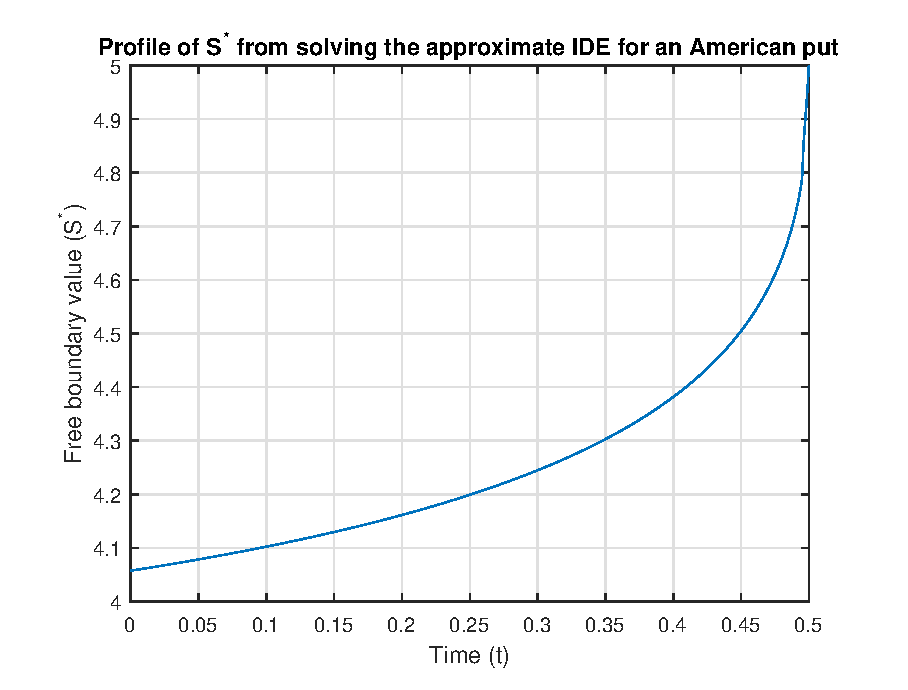
\includegraphics[scale=0.8]{figures/SfreePut.eps}
		\caption{The profile for $S^*$ from solving the approximate IDE~\eqref{eqn:SApproxPutLN} using $t=0$, $T=0.5$, $K = 5$, $r=0.05$, $q=0$, and $\sigma = 0.3$. The associated lognormal parameters are $\mu_Y = 0.9$, $\sigma_Y = 0.45$, and $\lambda = 0.1$.}
		\label{fig:amerputFreeBoundary}
	\end{figure}

\subsection{Results}
Here we will report the numerical outcomes from solving~\eqref{eqn:amerputjumpLNApprox} paired with solving the system for $S^*$~\eqref{eqn:SApproxPutLN}, \eqref{eqn:freePutTLN} against the FDM~\eqref{eqn:FDMPIDE}. Similar to the plot for $S^*$ that was displayed in the previous section, we will be employing the exact same parameter values. The financial parameters we will be using are $t=0$, $T=0.5$, $K = 5$, $r=0.05$, $q=0$, and $\sigma = 0.3$. The domain of $S_0$ (the underlying asset) will range from $10^{-3}$ to $4K$. This is done to emulate the scenarios of $S_0 \rightarrow 0$ and $S_0 \rightarrow \infty$. The jump-diffusion parameters are $\mu_Y = 0.9$, $\sigma_Y = 0.45$, and $\lambda = 0.1$. The simulations are done using MATLAB.

For the FDM, we use 101 spatial nodes and 501 temporal gridpoints. Consequently, this means we will also require 501 values of $S^*$ between $t=0$ and $t=0.5$. The domain of $S_0 \in [10^{-3},4K]$ will need to be divided into 100 equally-spaced subintervals to correspond to the 101 gridpoints used in the FDM. This is to ensure all resultant plots are consistent in terms of the input values used. For an American put option, we also require the following boundary conditions
	$$
		v_0^n = K, \quad v_I^n = 0, \quad \text{for all } n = 0,1,\ldots,N,
	$$
which correspond to the American put option at $S_0 \rightarrow 0$ and $S_0 \rightarrow \infty$ respectively for all time values in the domain. The option value curves are given in Figure~\ref{fig:amerputPlot} along with the absolute error between the two for the entire $S_0$ region. The MATLAB code for the FDM, the approximate IDE for $S^*$, and solving~\eqref{eqn:amerputjumpLNApprox} is available in the appendix with comments on how the code functions. Specifically, Appendix C.3 contains all that was used in this chapter.
	\begin{figure}[!h]
		\centering
		\subfigure[American put prices under jump-diffusion dynamics solved using the FDM scheme~\eqref{eqn:FDMPIDE} compared against~\eqref{eqn:amerputjumpLNApprox} with~\eqref{eqn:SApproxPutLN},~\eqref{eqn:freePutTLN} for the free boundary $S^*$. The price domain for the underlying asset is $(10^{-3},4K)$. The other financial parameters are $t=0$, $T=0.5$, $K = 5$, $r=0.05$, $q=0$, and $\sigma = 0.3$. \label{fig:amerputComp}]{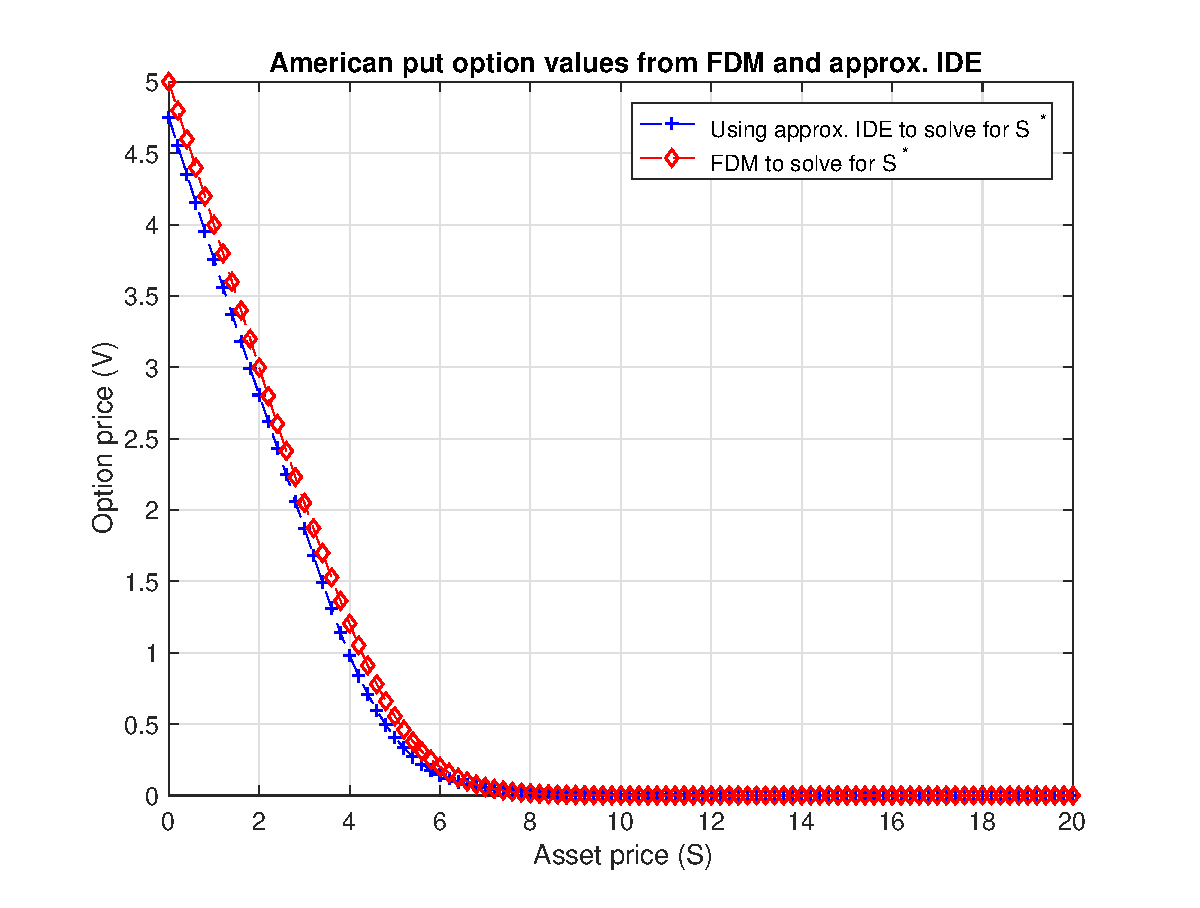
\includegraphics[width=0.7\linewidth]{figures/amerputFDMApprox.eps}\hspace*{3pt}}
		\subfigure[The absolute error between the FDM and using~\eqref{eqn:SApproxPutLN} for the American put values in a jump-diffusion model. \label{fig:amerputError}]{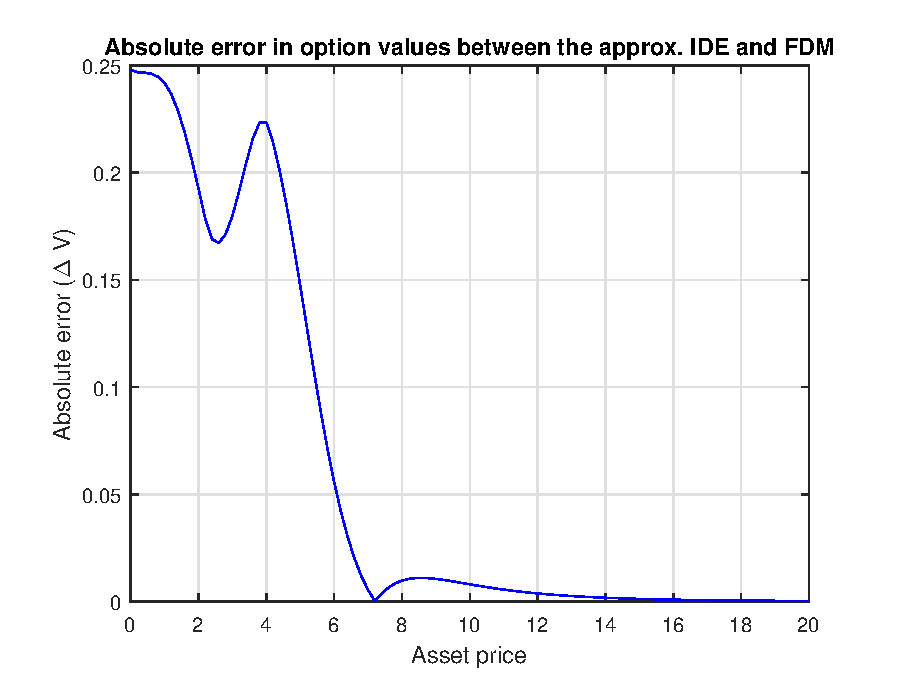
\includegraphics[width=0.7\linewidth]{figures/amerputFDMApproxError.eps}
			}
		\caption{American put value plots from the FDM and approximate IDE system using~\eqref{eqn:amerputjumpLNApprox},~\eqref{eqn:SApproxPutLN}, and~\eqref{eqn:freePutTLN}. The domain for the asset price is once again $(10^{-3},4K)$.}
		\label{fig:amerputPlot}
\end{figure}
 
From Figure~\ref{fig:amerputComp}, we can see that the American put option profiles overlap quite closely. Despite the assumptions that were made in order to simplify the pricing formula in~\eqref{eqn:amerputjumpLNApprox}, the errors that would have arose did not propagate to the resulting option values. This is highlighted in the absolute error between the option values in Figure~\ref{fig:amerputError} where the difference is only marginal.

\subsection{Conclusion}
In conclusion, we have derived an approximate IDE that enables us to solve for the optimal exercise boundary in a jump-diffusion model without the need to pair it with its corresponding option valuation formula. Furthermore, upon setting an approximate term for one of the integral terms for the American put option pricing formula, we were able to obtain an explicit approximation for the American put in jump-diffusion dynamics. The numerical reliability of these results were compared against the FDM to directly solve the Merton PIDE. Additionally the accuracy was acceptable for the given parameter values. Tentative future research could entail trialing different approximations for the integral term that appears in~\eqref{eqn:amerputjumpLNApprox} to make the pricing formula a better explicit approximate and also investigating the behaviour of such results when accounting for discrete dividend payments.
    \chapter[Alternative method for computing European compound options]{Alternative method for computing European compound options}
\chaptermark{European compound options}

\section{Outline}
This chapter will be outlined as follows. We will introduce the general compound options pricing formula in Section 6.2 with examples of application. This section also contains an interesting type of put-call parity that can occur for European vanilla compound options. In Section 6.3, we demonstrate the versatility of our pricing formula for a non-standard compound option. The variation to the pricing compound options when the underlying asset pays one discrete dividend is examined in Section 6.4. Closing remarks regarding these findings are provided in Section 6.5.

\section{Generalised compound option pricing formulas}
\label{sec:gen}
A compound option pricing formula for general payoffs will now be introduced. To begin, we first denote two options by $v_1$ and $v_2$ with payoffs $\phi_1$ and $\phi_2$ at expiry times $T_1$ and $T_2$, respectively. We also assume that $T_1 < T_2$. We now construct a compound option where $v_1$ has an underlying that is the second option $v_2$. We can express this mathematically from~\eqref{eqn:optionKernelSoln} to give
	\begin{equation}
		\label{eqn:v1aa}
		v_1(x,t) = \int_0^\infty \fr{1}{y}\K\left( \fr{x}{y}, t, T_1 \right)\phi_1(v_2(y,T_1)) \, \d y,
	\end{equation}
where
	\begin{equation}
		\label{eqn:v2a}
		v_2(y,T_1) = \int_0^\infty \fr{1}{z}\K\left( \fr{y}{z}, T_1, T_2 \right)\phi_2(z)\, \d z.
	\end{equation}
%With the aid of Corollary 1, it is possible to express all financial payoffs seen in options pricing and thus generate pricing formulas using~\eqref{eqn:v1aa} and~\eqref{eqn:v2a}.
We will illustrate how this works with the four standard European compound options.

\subsection{Call-on-a-call compound option}
A call-on-a-call option, denoted by $v_{\text{cc}}$, is composed of two European call options with two different strikes $K_1$ and $K_2$ and payoffs $\phi_1(x) = \max(x - K_1, 0)$ at $T_1$ and $\phi_2(x) = \max(x - K_2, 0)$ at $T_2$, respectively. Using \eqref{eqn:v1aa}, where we identify $v_1$ with $v_\mathrm{cc}$ and $v_2$ with $v_\mathrm{c}$, we obtain
	\begin{equation*}
		v_{\text{cc}}(x,t) = \int_0^\infty \fr{1}{y} \K\left( \fr{x}{y}, t, T_1 \right)\max(v_\text{c}(y,T_1; K_2, T_2) - K_1, 0)\, \d y.
	\end{equation*}
To proceed, we assume that $v_{\text{c}}(y,T_1; K_2, T_2) > K_1$ for all $y$ greater than some critical value $y_\mathrm{c}^*$~\cite{Kwok2008}. Due to the monotonicity of a European call with respect to the asset value, this critical value $y_\mathrm{c}^*$ will always be unique (see Figure~\ref{fig:1}). This simplifies the integral to
	\begin{align*}
		v_{\text{cc}}(x,t) &= \int_{y_\mathrm{c}^*}^\infty \fr{1}{y}\K\left( \fr{x}{y}, t, T_1 \right)[v_\text{c}(y,T_1; K_2, T_2) - K_1] \, \d y \\
		&= \int_{y_\mathrm{c}^*}^\infty \fr{1}{y} \K\left( \fr{x}{y}, t, T_1 \right)v_\text{c}(y,T_1; K_2, T_2) \, \d y - K_1\int_{y_\mathrm{c}^*}^\infty \fr{1}{y}\K\left( \fr{x}{y}, t, T_1 \right) \, \d y.
	\end{align*}

\begin{figure}[!h]
	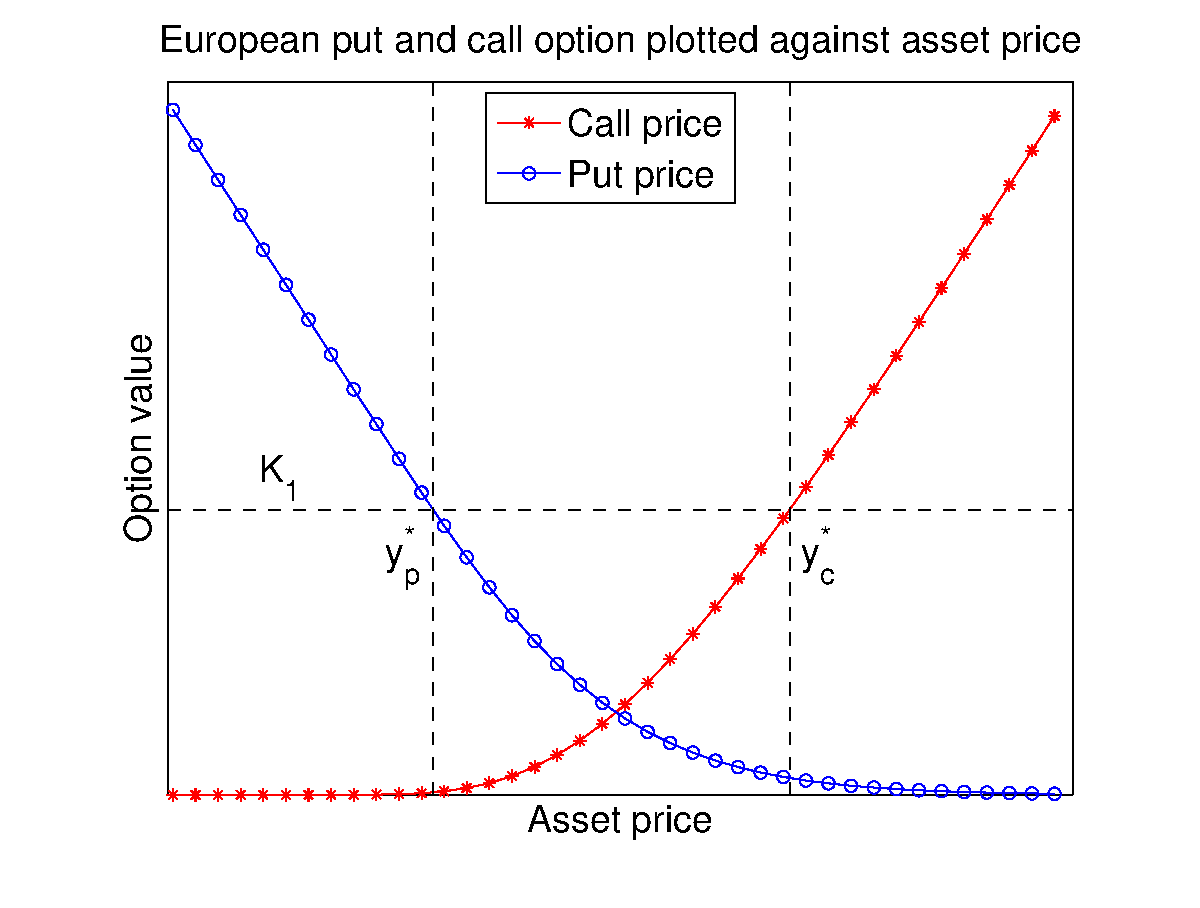
\includegraphics[scale=0.5]{figures/option.eps}
		\centering
		\caption{The European call~\eqref{eqn:EUcall} and European put~\eqref{eqn:EUput} plotted against $x$ for a fixed $t \in [0,T)$. The horizontal line that intersects both profiles is some strike price $K_1$ associated with the compound option. The intersection values correspond to the critical values ($y_\text{c}^*$ for a call and $y_\text{p}^*$ for a put) the underlying option must be below or above in order to have a positive payoff for the compound option.}
		\label{fig:1}
\end{figure}
\noindent
Using \eqref{eqn:optionKernelSoln} for $v_\text{c}$ gives
	\begin{align*}
		v_\text{cc}(x,t) &= \int_{y_\mathrm{c}^*}^\infty \fr{1}{y}\K\left( \fr{x}{y}, t, T_1 \right)\int_0^\infty \fr{1}{z} \K\left( \fr{y}{z}, T_1, T_2 \right)\max(z-K_2, 0) \, \d z \, \d y \\
		& \quad - K_1\int_{y_\mathrm{c}^*}^\infty \fr{1}{y}\K\left( \fr{x}{y}, t, T_1 \right) \, \d y \\
		&=  \int_{y_\mathrm{c}^*}^\infty \int_{K_2}^\infty \fr{1}{y}\K\left( \fr{x}{y}, t, T_1 \right)\K\left( \fr{y}{z}, T_1, T_2 \right) \, \d z \, \d y \\
		& \quad - K_2 \int_{y_\mathrm{c}^*}^\infty \int_{K_2}^\infty \fr{1}{y}\K\left( \fr{x}{y}, t, T_1 \right)\fr{1}{z}\K\left( \fr{y}{z}, T_1, T_2 \right) \, \d z \, \d y - K_1\int_{y_\mathrm{c}^*}^\infty \fr{1}{y}\K\left( \fr{x}{y}, t, T_1 \right) \, \d y.
	\end{align*}
We evaluate each integral using~\eqref{eqn:inta}\,--\,\eqref{eqn:int2} in Corollary 1 by choosing $a_1 = y_\mathrm{c}^*$, $b_1 = \infty$, $a_2 = K_2$, and $b_2 = \infty$. Using~\eqref{eqn:Nspecial}, we have
	\begin{equation}
		\label{eqn:vcc}
		\begin{split}
		v_\text{cc}(x,t) &=  xe^{-\int_t^{T_2} q(\tau) \, \d\tau}N_2\left( z_1\left( \fr{x}{y_\mathrm{c}^*}, t, T_1 \right), z_1\left( \fr{x}{K_2}, t, T_2 \right); \rho^* \right)  \\
		&\quad - K_2e^{-\int_t^{T_2} r(\tau) \, \d\tau} N_2\left( z_2\left( \fr{x}{y_\mathrm{c}^*}, t, T_1 \right), z_2\left( \fr{x}{K_2}, t, T_2 \right); \rho^* \right) \\
		&\quad - K_1e^{-\int_t^{T_1} r(\tau) \,\d\tau}N\left( z_2\left( \fr{x}{y_\mathrm{c}^*}, t, T_1 \right) \right),
		\end{split}
	\end{equation}
where
	\begin{equation}
		\label{eqn:rho2}
		\rho^* = \left(\fr{\int_t^{T_1} \sigma(\tau)^2 \, \d\tau}{\int_t^{T_2} \sigma(\tau)^2 \, \d\tau}\right)^{1/2}.
	\end{equation}
This agrees with the results derived by Geske~\cite{Geske1979} and Kwok~\cite{Kwok2008} who both implemented a probabilistic approach via a risk-neutral measure to compute the pricing formula.

\subsection{Put-on-a-put compound option}
In contrast to the call-on-a-call option, a put-on-a-put option $v_\mathrm{pp}$ comprises of a European put option with a strike $K_1$ and payoff $\phi_1(x) = \max(K_1-x,0)$ at $T_1$ with an underlying European put option with strike $K_2$ and payoff $\phi_2(x) = \max(K_2-x,0)$ at $T_2$. Using~\eqref{eqn:v1aa} where we identify $v_1$ with $v_\mathrm{pp}$ and $v_2$ with $v_\mathrm{p}$, we obtain
	$$
		v_\mathrm{pp}(x,t) = \int_0^\infty \fr{1}{y}\K\left( \fr{x}{y}, t, T_1 \right)\max(K_1 - v_\mathrm{p}(y,T_1;K_2,T_2), 0) \, \d y.
	$$
We want the values of $y$ such that $v_\mathrm{p}(y,T_1;K_2,T_2) < K_1$ to ensure a strictly positive argument for the payoff $\phi_1$. According to Figure~\ref{fig:1}, this corresponds to $y > y_\mathrm{p}^*$. Although the European put option profile also exhibits monotonic (decreasing) behaviour, there is an extra restriction for $y_\mathrm{p}^*$ to be unique. At $y=0$, the underlying put option will be
	$$
		v_\text{p}(0,T_1) = K_2e^{-\int_{T_1}^{T_2} r(\tau) \, \d\tau}.
	$$
	In order for $y_\text{p}^*$ to be unique, we require
	\begin{equation}
		\label{eqn:pprestriction}
		K_1 \leq K_2e^{-\int_{T_1}^{T_2} r(\tau) \, \d\tau},
	\end{equation}
	since the intersection of $K_1$ with the option profile will represent the critical value for the compound option. If $K_1 > K_2e^{-\int_{T_1}^{T_2} r(\tau) \, \d\tau}$, there will be no intersection with the European put option curve and thus no critical value for the compound option.

Substituting $v_\mathrm{p}$ for its integral expression using~\eqref{eqn:optionKernelSoln}, we have
	\begin{align*}
		v_\text{pp}(x,t) &= K_1\int_{y_\mathrm{p}^*}^\infty \fr{1}{y}\K\left( \fr{x}{y}, t, T_1 \right) \, \d y \\
		&\quad - \int_{y_\mathrm{p}^*}^\infty \fr{1}{y}\K\left( \fr{x}{y}, t, T_1 \right)\int_0^\infty \fr{1}{z} \K\left( \fr{y}{z}, T_1, T_2 \right)\max(K_2-z, 0) \, \d z \, \d y 		\\
		&=  K_1\int_{y_\mathrm{p}^*}^\infty \fr{1}{y}\K\left( \fr{x}{y}, t, T_1 \right) \, \d y - K_2 \int_{y_\mathrm{p}^*}^\infty \int_{0}^{K_2} \fr{1}{y}\K\left( \fr{x}{y}, t, T_1 \right)\fr{1}{z}\K\left( \fr{y}{z}, T_1, T_2 \right) \, \d z \, \d y \\
		&\quad +  \int_{y_\mathrm{p}^*}^\infty \int_{0}^{K_2} \fr{1}{y}\K\left( \fr{x}{y}, t, T_1 \right)\K\left( \fr{y}{z}, T_1, T_2 \right) \, \d z \, \d y.
	\end{align*}
Once again, each integral is evaluated using~\eqref{eqn:inta}\,--\,\eqref{eqn:int2} in Corollary 1 and simplified using~\eqref{eqn:Nspecial}. Choosing $a_1 = y_\mathrm{p}^*$, $b_1 = \infty$, $a_2 = 0$, and $b_2 = K_2$ yields
	\begin{align}
		v_\text{pp}(x,t) &=  K_2e^{-\int_t^{T_2} r(\tau) \, \d\tau}\left[ N_2\left( z_2\left( \fr{x}{y_\mathrm{p}^*}, t, T_1 \right), z_2\left( \fr{x}{K_2}, t, T_2 \right); \rho^* \right) - N\left(z_2\left( \fr{x}{y_\text{p}^*},t, T_1 \right)\right)\right] \nonumber \\ %\label{eqn:vpp}  \\ \\
		&\quad - xe^{-\int_t^{T_2} q(\tau) \, \d\tau}\left[ N_2\left( z_1\left( \fr{x}{y_\text{p}^*}, t, T_1 \right), z_1\left( \fr{x}{K_2}, t, T_2 \right); \rho^* \right) - N\left(z_1\left( \fr{x}{y_\text{p}^*},t, T_1 \right)\right)\right] \nonumber \\
		&\quad + K_1e^{-\int_t^{T_1} r(\tau) \,\d\tau}N\left( z_2\left( \fr{x}{y_\text{p}^*}, t, T_1 \right) \right), \nonumber
	\end{align}
where $\rho^*$ is the same as in~\eqref{eqn:rho2}.

\subsection{Call-on-a-put compound option}
We will use~$v_\mathrm{cp}$ for the value of a call-on-a-put compound option. This is made up of a European call option with a strike price $K_1$ and payoff $\phi_1(x) = \max(x-K_1,0)$ at $T_1$ with an underlying European put option with strike $K_2$ and payoff $\phi_2(x) = \max(K_2-x,0)$ at $T_2$.  From~\eqref{eqn:v1aa}, we associate $v_1$ with $v_\mathrm{cp}$ and $v_2$ with $v_\mathrm{p}$ to get
	$$
		v_\mathrm{cp}(x,t) = \int_0^\infty \fr{1}{y}\K\left( \fr{x}{y}, t, T_1 \right)\max(v_\mathrm{p}(y,T_1;K_2,T_2) - K_1, 0) \, \d y.
	$$
We assume the $v_\mathrm{p}(y,T_1;K_2,T_1) > K_1$ to ensure that the payoff $\phi_1$ is positive. However in contrast to the previous examples, we need to be \emph{below} the critical value $y_\text{p}^*$ (since the underlying is a put option) in order to achieve this (see Figure~\ref{fig:1}). We also express $v_\text{p}$ in integral form using~\eqref{eqn:optionKernelSoln} which leaves us with
		\begin{align*}
		v_\text{cp}(x,t) &= \int_{0}^{y_\mathrm{p}^*} \fr{1}{y}\K\left( \fr{x}{y}, t, T_1 \right)\int_0^\infty \fr{1}{z} \K\left( \fr{y}{z}, T_1, T_2 \right)\max(K_2-z, 0) \, \d z \, \d y \\
		& \quad - K_1\int_{0}^{y_\mathrm{p}^*} \fr{1}{y}\K\left( \fr{x}{y}, t, T_1 \right) \, \d y \\
		&=  K_2\int_{0}^{y_\mathrm{p}^*} \int_{0}^{K_2} \fr{1}{y}\K\left( \fr{x}{y}, t, T_1 \right)\fr{1}{z}\K\left( \fr{y}{z}, T_1, T_2 \right) \, \d z \, \d y \\
		& \quad - \int_{0}^{y_\mathrm{p}^*} \int_0^{K_2} \fr{1}{y}\K\left( \fr{x}{y}, t, T_1 \right)\K\left( \fr{y}{z}, T_1, T_2 \right) \, \d z \, \d y - K_1\int_{0}^{y_\mathrm{p}^*} \fr{1}{y}\K\left( \fr{x}{y}, t, T_1 \right) \, \d y,
	\end{align*}
where we still assume~\eqref{eqn:pprestriction} to ensure uniqueness for $y_\text{p}^*$. Using Corollary 1 with $a_1 = 0$, $b_1 = y_\mathrm{p}^*$, $a_2 = 0$, and $b_2 = K_2$ and upon simplifying all the $N$ and $N_2$ terms using~\eqref{eqn:Nspecial}, we get	\begin{equation}
		\label{eqn:vcp}
		\begin{split}
		v_\text{cp}(x,t) &= v_\text{pp}(x,t) + v_\text{p}(x,t;K_2,T_2) - K_1e^{-\int_t^{T_1} r(\tau) \, \d\tau}.
		\end{split}
	\end{equation}
Eq.~\eqref{eqn:vcp} behaves like a pseudo-put-call parity between $v_\text{pp}$ and $v_\text{cp}$. It should be highlighted that this equation bares a strong similarity to the standard put-call parity result~\eqref{eqn:pcp}. We will witness a similar occurrence for a put-on-a-call compound option next.
	
\subsection{Put-on-a-call compound option}
The final standard combination is a put-on-a-call compound option, which we will label $v_\text{pc}$. This option is constructed with a European put option with strike $K_1$ and payoff $\phi_1(x) = \max(K_1-x,0)$ at $T_1$ with an underlying European call option with strike $K_2$ and payoff $\phi_2(x) = \max(x-K_2,0)$ at $T_2$. Setting $v_1$ to $v_\text{pc}$ and $v_2$ to $v_\text{c}$ in~\eqref{eqn:v1aa} results in

\begin{equation*}
		v_{\text{pc}}(x,t) = \int_0^\infty \fr{1}{y} \K\left( \fr{x}{y}, t, T_1 \right)\max(K_1 -v_\text{c}(y,T_1; K_2, T_2), 0)\, \d y.
	\end{equation*}
For $v_{\text{c}}(y,T_1; K_2, T_2) < K_1$ to be satisfied and guarantee a positive payoff $\phi_1$, we need to be below $y_\text{c}^*$ according to Figure~\ref{fig:1} (since the option being compounded on is a European call). This simplifies  to
	\begin{align*}
		v_\text{pc}(x,t) &= K_1\int_{0}^{y_\mathrm{c}^*} \fr{1}{y}\K\left( \fr{x}{y}, t, T_1 \right) \, \d y - \int_{0}^{y_\mathrm{c}^*} \fr{1}{y} \K\left( \fr{x}{y}, t, T_1 \right)v_\text{c}(y,T_1; K_2, T_2) \, \d y.
	\end{align*}
Once again incorporating \eqref{eqn:optionKernelSoln} for $v_\text{c}$ leads to
	\begin{align*}
		v_\text{pc}(x,t) &= K_1\int_{0}^{y_\mathrm{c}^*} \fr{1}{y}\K\left( \fr{x}{y}, t, T_1 \right) \, \d y \\
		&\quad - \int_0^{y_\mathrm{c}^*}\fr{1}{y}\K\left( \fr{x}{y}, t, T_1 \right)\int_0^\infty \fr{1}{z} \K\left( \fr{y}{z}, T_1, T_2 \right)\max(z-K_2,0) \, \d z \, \d y \\
		&= K_1\int_{0}^{y_\mathrm{c}^*} \fr{1}{y}\K\left( \fr{x}{y}, t, T_1 \right) \, \d y - \int_0^{y_\mathrm{c}^*}\int_{K_2}^\infty \fr{1}{y}\K\left( \fr{x}{y},t,T_1 \right)\K\left( \fr{y}{z}, T_1, T_2 \right) \, \d z \, \d y \\
		&\quad + K_2\int_0^{y_\mathrm{c}^*}\int_{K_2}^\infty\fr{1}{y}\K\left( \fr{x}{y}, t, T_1 \right) \fr{1}{z} \K\left( \fr{y}{z}, T_1, T_2 \right) \d z \, \d y .
	\end{align*}
Choosing $a_1 = 0$, $b_1 = y_\mathrm{c}^*$, $a_2 = K_2$, and $b_2 = \infty$ for Corollary 1 will give
\begin{equation}
		\label{eqn:vpc}
		\begin{split}
		v_\text{pc}(x,t) &= v_\text{cc}(x,t) - v_\text{c}(x,t;K_2,T_2) + K_1e^{-\int_t^{T_1} r(\tau) \, \d\tau},
		\end{split}
	\end{equation}
where $\rho^*$ is as in~\eqref{eqn:rho2} and~\eqref{eqn:Nspecial} was used to simplify the $N$ and $N_2$ terms. This is the pseudo-put-call parity relation between $v_\text{cc}$ and $v_\text{pc}$. It should be stressed the critical values $y_\text{c}^*$ and $y_\text{p}^*$ may not necessarily be equal, thus a put-call parity relating $v_\text{cc}$ and $v_\text{pp}$ without a dependence on $v_\text{pc}$ and $v_\text{cp}$ is unlikely to be ascertained unless in special circumstances (e.g., $y_\text{c}^* = y_\text{p}^*$). However, adding~\eqref{eqn:vcp} to~\eqref{eqn:vpc} and rearranging gives us
	\begin{equation*}
		v_\text{cc}(x,t) + v_\text{pp}(x,t) = v_\text{pc}(x,t) + v_\text{cp}(x,t) + v_\text{c}(x,t; K_2, T_2) - v_\text{p}(x,t; K_2, T_2)
	\end{equation*}
Now using~\eqref{eqn:pcp}, we can relate $v_\text{c}(x,t; K_2, T_2)$ to $v_\text{p}(x,t; K_2, T_2)$ and obtain
	\begin{equation}
		\label{eqn:pseudopcp}
		v_\text{cc}(x,t) + v_\text{pp}(x,t) =  v_\text{pc}(x,t) + v_\text{cp}(x,t) + xe^{-\int_t^{T_2} q(\tau) \, \d\tau} - K_2e^{-\int_t^{T_2} r(\tau) \, \d\tau},
	\end{equation}
which resembles the standard put-call parity identity in~\eqref{eqn:pcp} in form. Another interesting route would have been to incorporate a portfolio argument to arrive at~\eqref{eqn:pseudopcp}, but we opted for our presented approach as it ties in closely with the results from this work.

\section{Generalised example: straddle-on-a-call compound option}
We outlined in Section~\ref{sec:gen} that the results in Corollary 1 can be implemented for any financial payoff in options pricing to generate any compound option pricing formula. This is attainable since any of the aforementioned payoffs can be expressed as finite linear combinations of the functions
	\begin{equation}
		\label{eqn:funcs}
		x \mapsto \1_I(x), \quad x \mapsto x\1_I(x),
	\end{equation}
where $\1_I$ is the indicator function defined as
	\begin{equation*}
		\1_I(x) = \begin{cases}
			1, \quad x \in I, \\
			0, \quad x \notin I,
		\end{cases}
	\end{equation*}
and where $I$ is an arbitrary interval with endpoints $a$ and $b$ with $a < b$. The interval can be open, half-closed, or closed. \textcolor{black}{The two auxiliary functions in~\eqref{eqn:funcs} are the building blocks for many financial payoffs in options pricing.} For example, a call option has a payoff $\max(x-K,0)$ which can be written as
	\begin{equation*}
		\max(x-K,0) = x\1_{[K,\infty)}(x) - K\1_{[K,\infty)}(x),
	\end{equation*}
where the interval $I$ is $[K,\infty)$.

In general, there are four possibilities for the auxiliary functions to consider in compound options:
	\begin{enumerate}
		\item $\phi_1(x) = \1_I(x)$, $\phi_2(x) = \1_I(x)$,
		\item $\phi_1(x) = \1_I(x)$, $\phi_2(x) = x\1_I(x)$,
		\item $\phi_1(x) = x\1_I(x)$, $\phi_2(x) = \1_I(x)$,
		\item $\phi_1(x) = x\1_I(x)$, $\phi_2(x) = x\1_I(x)$.
	\end{enumerate}
Using~\eqref{eqn:v1aa} and~\eqref{eqn:v2a}, it can be shown that the first two cases when used will result in~\eqref{eqn:inta} upon evaluation; \eqref{eqn:int1} will be the result when using the third case; and computation using the fourth possibility will yield \eqref{eqn:int2}. To highlight the flexibility and generality of~\eqref{eqn:funcs}, we will look at pricing a straddle-on-a-call option.

To set this up, we require two options: an outer straddle option with payoff $\max(x-K_1,0) + \max(K_1-x,0)$ at $t = T_1$, and an inner call option with payoff $\max(x-K_2,0)$ at $t = T_2$. We will denote a straddle by $v_{\text{s}}$ and the compound option by $v_{\text{sc}}$. So we have
	\begin{align*}
		v_\text{sc}(x,t) &= \int_0^\infty \fr{1}{y}\K\left( \fr{x}{y}, t, T_1 \right)\left[\max(v_\text{c}(y,T_1) - K_1, 0) + \max(K_1 - v_\text{c}(y,T_1), 0) \right] \, \d y.
	\end{align*}
Upon splitting up the terms, we notice we have the two integrals that formulate a call-on-a-call compound option and a put-on-a-call compound option, respectively. Thus,
	\begin{equation}
		\label{eqn:vsc}
			v_\text{sc}(x,t) = v_\text{cc}(x,t) + v_\text{pc}(x,t).
	\end{equation}
	
\section{Compound options with discrete dividends}
Up until now, the model we have presented for pricing compound options assumes a continuous dividend yield for the lifetime of the options. That is, $q$ is a time-continuous function. Here we introduce a technique to formulate compound options when the underlying asset pays one dividend yield at a fixed time. What we will show is that it is only one slight variation needed to the methodology used to derive all the previous formulas.

The underlying asset with a potential dividend yield (whether discrete or continuous) is governed by~\cite{Wilmott1995}
	\begin{equation*}
		%\label{eqn:SDE2}
		\d S_t = [r(t)S_t - D(S_t,t)] \, \d t + \sigma(t) S_t  \, \d W_t,
	\end{equation*}
where $D(S_t,t)$ does not necessarily to have be linear in $S_t$. It follows that a European option whose underlying follows the SDE above satisfies
	\begin{equation*}
		\fr{\pr v}{\pr t} + \fr{1}{2}\sigma(t)^2x^2\fr{\pr^2 v}{\pr x^2} + [r(t)x - D(x,t)]\fr{\pr v}{\pr x} - r(t)v = 0.
	\end{equation*}
This is a potential unified approach to pricing options regardless of whether the dividend yield is continuous or discrete. However, the Black-Scholes kernel identities in the preliminaries rely on the dividend term $D$ being linear in $x$ (i.e., $D(x,t) = q(t)x$). Therefore, in order to adapt the kernel identities, we have assumed a specific form for $D$ to be able to construct a pricing formula for discrete dividends.

To proceed, we assume a dividend of value proportional to the asset price is paid out on a date $t = t_d$, where $t_d$ is before the expiry. Consequently, this means that the asset price $S_t$ will decrease by a proportion of its value as it passes $t_d$. We call the proportion factor $q_d \in [0,1)$. Using $t_d^-$ and $t_d^+$ to indicate an infinitesimal time before and after the dividend payment date, respectively, mathematically this implies the following jump condition
	\begin{equation}
		\label{eqn:jumpcond}
		S_{t_d^+} = S_{t_d^-} - q_dS_{t_d^-} = (1-q_d)S_{t_d^-}.
	\end{equation}
A common way to price options when the underlying pays a discrete dividend is to solve the Black-Scholes equation~\eqref{eqn:blackscholes} backwards in time twice; once from expiry $T$ to $t_d^+$ and then from $t_d^-$ to an arbitrary time $t$~\cite{Wilmott1995, Jiang2005}. However, an extra step is required whereby the jump condition~\eqref{eqn:jumpcond} for $S_t$ needs to be accounted for as a boundary condition between $t_d^+$ and $t_d^-$.

We will first illustrate this concept of discrete dividend payments in a standard European option with payoff $\phi$. Suppose one dividend is paid at time $t_d \in (0,T)$. Once again, we denote $t_d^-$ and $t_d^+$ to be the moment before and after the dividend payment is made, respectively. Working backwards from $T$ to $t_d^+$, we define a function $w$ to be
		$$
			w(x,t) = \int_0^\infty \fr{1}{y} \K\left( \fr{x}{y},t, T \right)\phi(y) \, \d y, \quad t_d^+ \leq t \leq T,
		$$
where we used~\eqref{eqn:optionKernelSoln}. From the jump condition~\eqref{eqn:jumpcond}, we have
		$$
			w\left(S_{t_d^-},t_d^-\right) = w\left(S_{t_d^+},t_d^+\right) = w\left((1-q_d)S_{t_d^-},t_d^+\right).
		$$
This expression acts as our payoff from $t_d^-$ backwards to time-zero since it is the matching condition between $t_d^+$ and $t_d^-$. Therefore,
		\begin{equation}
			\label{eqn:cool}
			v(x,t) =
			\begin{cases}
				\ds\int_0^\infty \fr{1}{y} \K\left( \fr{x}{y}, t, t_d^- \right)w\left( (1-q_d)y, t_d^+ \right) \, \d y & \text{if } 0 \leq t \leq t_d^-, \\
				\ds\int_0^\infty \fr{1}{y} \K\left( \fr{x}{y}, t, T \right) \phi(y) \, \d y = w(x,t) & \text{if } t_d^+ \leq t \leq T.
			\end{cases}
		\end{equation}
For compound options paying only one discrete dividend, we have three cases to consider since we have two terminal dates $T_1$ and $T_2$ ($T_1 < T_2$) for the compound and underlying option, respectively. We assume that $0 < t_d < T_2$.

\subsection{Case 1: $0 < t_d < T_1 < T_2$}
In this scenario, we assume that the dividend payment is before the terminal date of the compound option (see Figure~\ref{fig:2}).

\begin{figure}[!h]
\centering
\begin{tikzpicture}
\draw (0,0) -- (8,0);
\draw (0pt,8pt) -- (0pt,-8pt) node[below,fill=white] {0};
\draw[xshift=1cm] (0pt,4pt) -- (0pt,-4pt) node[below,fill=white] {$t_d^-$};
\draw[xshift=2cm] (0pt,4pt) -- (0pt,-4pt) node[below,fill=white] {$t_d$};
\draw[xshift=3cm] (0pt,4pt) -- (0pt,-4pt) node[below,fill=white] {$t_d^+$};
\draw[xshift=4cm] (0pt,8pt) -- (0pt,-8pt) node[below,fill=white] {$T_1$};
\draw[xshift=8cm] (0pt,8pt) -- (0pt,-8pt) node[below,fill=white] {$T_2$};
\end{tikzpicture}
\caption{The dividend is paid on the date $t_d$ which is before the expiry $T_1$ of the compound option.}
\label{fig:2}
\end{figure}
\noindent
Working backwards from $T_1$ to $t_d^+$, we first define $w_1$ to be
		\begin{equation}
			\label{eqn:w1}
			w_1(x,t) = \int_0^\infty \fr{1}{y} \K\left( \fr{x}{y}, t, T_1 \right) \phi_1(v_2(y,T_1)) \, \d y, \quad t_d^+ \leq t \leq T_1,
		\end{equation}
where
		\begin{equation}
			\label{eqn:v2}
			v_2(y,T_1) = \int_0^\infty \fr{1}{z} \K\left( \fr{y}{z}, T_1, T_2 \right) \phi_2(z) \, \d z.
		\end{equation}
Equation~\eqref{eqn:w1} is valid since between $t_d^+$ and $T_1$, the compound option has not yet expired. Using~\eqref{eqn:jumpcond} to match across the boundary $t_d^+$ gives
		$$
			w_1\left(S_{t_d^-},t_d^-\right) = w_1\left(S_{t_d^+},t_d^+\right) = w_1\left((1-q_d)S_{t_d^-},t_d^+\right).
		$$
	Then for $0 \leq t \leq t_d^-$, we have
		$$
			v_1(x,t) = \int_0^\infty \fr{1}{y}\K\left( \fr{x}{y}, t, t_d^- \right)w_1\left((1-q_d)y, t_d^+\right) \, \d y.
		$$
	Thus the compound option $v_1$ is given by
		\begin{equation}
			\label{eqn:v1}
			v_1(x,t) =
			\begin{cases}
				\ds\int_0^\infty \fr{1}{y} \K\left( \fr{x}{y}, t, t_d^- \right)w_1\left( (1-q_d)y, t_d^+ \right) \, \d y & \text{if } 0 \leq t \leq t_d^-, \\
				\ds\int_0^\infty \fr{1}{y} \K\left( \fr{x}{y}, t, T_1 \right) \phi_1(v_2(y,T_1)) \, \d y & \text{if } t_d^+ \leq t \leq T_1,
			\end{cases}
		\end{equation}
	with $v_2$ defined as in \eqref{eqn:v2}.
In this case, the compound option needs to be ``segmented'' in a piecewise manner since the dividend payment date $t_d$ is situated before $T_1$ (i.e., during the compound option's lifespan). We will see in the next scenario how the location of $t_d$ changes the formula for a compound option under one discrete dividend payment.
	
\subsection{Case 2: $0 < T_1 < t_d < T_2$}
We also consider the circumstance where the dividend payment happens after the compound option has expired but before the expiry date of the underlying option it acts upon (see Figure~\ref{fig:3}).

\begin{figure}[!h]
\centering
\begin{tikzpicture}
\draw (0,0) -- (8,0);
\draw (0pt,8pt) -- (0pt,-8pt) node[below,fill=white] {0};
\draw[xshift=4cm] (0pt,8pt) -- (0pt,-8pt) node[below,fill=white] {$T_1$};
\draw[xshift=5cm] (0pt,4pt) -- (0pt,-4pt) node[below,fill=white] {$t_d^-$};
\draw[xshift=6cm] (0pt,4pt) -- (0pt,-4pt) node[below,fill=white] {$t_d$};
\draw[xshift=7cm] (0pt,4pt) -- (0pt,-4pt) node[below,fill=white] {$t_d^+$};
\draw[xshift=8cm] (0pt,8pt) -- (0pt,-8pt) node[below,fill=white] {$T_2$};
\end{tikzpicture}
\caption{The dividend is paid on the date $t_d$ after $T_1$, which is past the lifetime of the compound option but still before the expiry of the underlying option.}
\label{fig:3}
\end{figure}
\noindent
In this formulation, the underlying option will need to be expressed piecewise in contrast to the piecewise compound option~\eqref{eqn:v1}. Once again working backwards from $T_2$ to $t_d^+$, we define $w_2$ to be
		$$
			w_2(x,t) = \int_0^\infty \fr{1}{y}\K\left( \fr{x}{y}, t, T_2 \right)\phi_2(y) \, \d y, \quad t_d^+ \leq t \leq T_2.
		$$
The jump condition~\eqref{eqn:jumpcond} gives
		$$
			w_2\left(S_{t_d^-},t_d^-\right) = w_2\left(S_{t_d^+},t_d^+\right) = w_2\left((1-q_d)S_{t_d^-},t_d^+\right).
		$$
Then for $T_1 \leq t \leq t_d^-$, we have
		$$
			v_2(x,t) = \int_0^\infty \fr{1}{y} \K\left( \fr{x}{y}, t, t_d^- \right)w_2\left( (1-q_d)y, t_d^+ \right) \, \d y.
		$$
Therefore $v_2$ is given by
		\begin{equation}
			v_2(x,t) =
			\begin{cases}
				\ds\int_0^\infty \fr{1}{y} \K\left( \fr{x}{y}, t, t_d^- \right)w_2\left( (1-q_d)y, t_d^+ \right) \, \d y & \text{if } T_1 \leq t \leq t_d^-, \\
				\ds\int_0^\infty \fr{1}{y} \K\left( \fr{x}{y}, t, T_2 \right) \phi_2(y) \, \d y = w_2(x,t) & \text{if } t_d^+ \leq t \leq T_2.
			\end{cases}
		\end{equation}
Now for $0 \leq t \leq T_1$, the compound option $v_1$ will be
		\begin{equation}
			\label{eqn:v1a}
			v_1(x,t) = \int_0^\infty \fr{1}{y} \K\left( \fr{x}{y}, t, T_1 \right)\phi_1(v_2(y,T_1))\, \d y.
		\end{equation}

\subsection{Case 3: $0 < t_d = T_1 < T_2$}
The last possible case is when the dividend payment is issued on the expiry date of the compound option (see Figure~\ref{fig:4}). As we will see, this unfolds to be quite an easy solution.

\begin{figure}[!h]
\centering
\begin{tikzpicture}
\draw (0,0) -- (8,0);
\draw (0pt,8pt) -- (0pt,-8pt) node[below,fill=white] {0};
\draw[xshift=3cm] (0pt,4pt) -- (0pt,-4pt) node[below,fill=white] {$t_d^-$};
\draw[xshift=4cm] (0pt,8pt) -- (0pt,-8pt) node[below,fill=white] {$t_d = T_1$};
\draw[xshift=5cm] (0pt,4pt) -- (0pt,-4pt) node[below,fill=white] {$t_d^+$};
\draw[xshift=8cm] (0pt,8pt) -- (0pt,-8pt) node[below,fill=white] {$T_2$};
\end{tikzpicture}
\caption{The dividend is paid on the date the compound option expires, which implies that $t_d = T_1$.}
\label{fig:4}
\end{figure}
\noindent
Working backwards from $T_2$ to $t_d^+$, we have
		\begin{equation}
			\label{eqn:v2b}
			v_2(x,t) = \int_0^\infty \fr{1}{z} \K\left( \fr{x}{z}, t, T_2 \right) \phi_2(y) \, \d y, \quad t_d^+ \leq t \leq T_2.
		\end{equation}
Using~\eqref{eqn:jumpcond} to match the boundaries, we get
		$$
			v_2\left(S_{t_d^-},t_d^-\right) = v_2\left(S_{t_d^+},t_d^+\right) = v_2\left((1-q_d)S_{t_d^-},t_d^+\right),
		$$
which gives us
		\begin{equation}
			\label{eqn:v1c}
			v_1(x,t) = \int_0^\infty \fr{1}{y} \K\left( \fr{x}{y}, t, t_d^- \right) v_2((1-q_d)y, t_d^+) \, \d y, \quad 0 \leq t \leq t_d^-.
		\end{equation}

\subsection{Example: Call-on-a-call for $0 < t_d < T_1 < T_2$}
We will now demonstrate how to apply one of the aforementioned general formulas in a discrete dividend setting to a European call-on-a-call compound option assuming Case 1. Using~\eqref{eqn:v1}, for $t_d^+ \leq t \leq T_1$, we just have a standard call-on-a-call since the dividend has been paid. We define a function $w_\text{cc}$ to represent this and it gives
	\begin{equation*}
		\begin{split}
		w_\text{cc}(x,t) &=  \int_{y_\mathrm{c}^*}^\infty \int_{K_2}^\infty \fr{1}{y}\K\left( \fr{x}{y}, t, T_1 \right)\K\left( \fr{y}{z}, T_1, T_2 \right) \, \d z \, \d y \\
		& \quad - K_2 \int_{y_\mathrm{c}^*}^\infty \int_{K_2}^\infty \fr{1}{y}\K\left( \fr{x}{y}, t, T_1 \right)\fr{1}{z}\K\left( \fr{y}{z}, T_1, T_2 \right) \, \d z \, \d y - K_1\int_{y_\mathrm{c}^*}^\infty \fr{1}{y}\K\left( \fr{x}{y}, t, T_1 \right) \, \d y,
	\end{split}
	\end{equation*}
recalling the integral expression before~\eqref{eqn:vcc}, where $y_\mathrm{c}^*$ is the associated critical value and $\rho^*$ is defined in~\eqref{eqn:rho2}. For notational simplicity, we define $\alpha = 1-q_d$. Then for $0 \leq t \leq t_d^-$, we use the first part of~\eqref{eqn:v1} to get
		\begin{equation*}
			\begin{split}
				v_\text{cc}(x,t) &= \int_0^\infty \fr{1}{y}\K\left( \fr{x}{y}, t, t_d^- \right)w_\text{cc}\left( \alpha y, t_d^+ \right) \, \d y \\
				&= \int_0^\infty \int_{y_\mathrm{c}^*}^\infty \int_{K_2}^\infty \fr{1}{y}\K\left( \fr{x}{y}, t, t_d^- \right) \fr{1}{z}\K\left( \fr{\alpha y}{z}, t_d^+, T_1 \right)\K\left( \fr{z}{w}, T_1, T_2 \right) \, \d w \, \d z \, \d y \\
				&\quad - K_2\int_0^\infty \int_{y_\mathrm{c}^*}^\infty \int_{K_2}^\infty \fr{1}{y}\K\left( \fr{x}{y}, t, t_d^- \right) \fr{1}{z}\K\left( \fr{\alpha y}{z}, t_d^+, T_1 \right)\fr{1}{w}\K\left( \fr{z}{w}, T_1, T_2 \right) \, \d w \, \d z \, \d y \\
				&\quad - K_1\int_0^\infty \int_{y_\mathrm{c}^*}^\infty \fr{1}{y}\K\left( \fr{x}{y}, t, t_d^- \right) \fr{1}{z}\K\left( \fr{\alpha y}{z}, t_d^+, T_1 \right) \, \d z \, \d y \\
				&= I_1 + I_2 + I_3.
			\end{split}
		\end{equation*}
Looking at $I_1$, the triple integral is in fact iterated. Therefore we arrange the order of integration with respect to $y$ first, then
		\begin{align*}
			I_1 &=  \int_{y_\mathrm{c}^*}^\infty \int_{K_2}^\infty \fr{1}{z} \K\left( \fr{z}{w}, T_1, T_2 \right)\int_0^\infty \fr{1}{y}\K\left( \fr{x}{y}, t, t_d^- \right) \K\left( \fr{\alpha y}{z}, t_d^+, T_1 \right) \, \d y \, \d w \, \d z \\
			& =\int_{y_\mathrm{c}^*}^\infty \int_{K_2}^\infty \fr{1}{z} \K\left( \fr{z}{w}, T_1, T_2 \right)\K_d\left( \fr{\alpha x}{z}, t, t_d^-, t_d^+, T_1 \right) \,  \d w \, \d z,
		\end{align*}
where~\eqref{eqn:intlem1} was implemented to simplify the innermost integral. Now using~\eqref{eqn:cor2c} in conjunction with~\eqref{eqn:Nspecial}, we obtain
	$$
		I_1 = \alpha xe^{-\int_t^{t_d^-} q(\tau) \, \d\tau - \int_{t_d^+}^{T_2} q(\tau)\,\d\tau}N_2\left( y_1\left( \fr{\alpha x}{y_\text{c}^*}, t, t_d^-, t_d^+, T_1 \right), y_1\left( \fr{\alpha x}{K_2}, t, t_d^-, t_d^+, T_2 \right); \rho_d^* \right),
	$$
where
	$$
		\rho_d^* = \left[ \fr{\int_t^{t_d^-} \sigma(\tau)^2 \,\d\tau + \int_{t_d^+}^{T_1} \sigma(\tau)^2 \, \d\tau}{\int_t^{t_d^-} \sigma(\tau)^2 \,\d\tau + \int_{t_d^+}^{T_2} \sigma(\tau)^2 \,\d\tau} \right].
	$$
For $I_2$, we do a similar process but incorporate~\eqref{eqn:cor2b} with~\eqref{eqn:Nspecial} to give
	\begin{align*}
		 I_2 &=  -K_2\int_{y_\mathrm{c}^*}^\infty \int_{K_2}^\infty \fr{1}{zw} \K\left( \fr{z}{w}, T_1, T_2 \right)\int_0^\infty \fr{1}{y}\K\left( \fr{x}{y}, t, t_d^- \right) \K\left( \fr{\alpha y}{z}, t_d^+, T_1 \right) \, \d y \, \d w \, \d z \\
			& =-K_2\int_{y_\mathrm{c}^*}^\infty \int_{K_2}^\infty \fr{1}{w} \K\left( \fr{z}{w}, T_1, T_2 \right)\fr{1}{z}\K_d\left( \fr{\alpha x}{z}, t, t_d^-, t_d^+, T_1 \right) \,  \d w \, \d z \\
			&= -K_2e^{-\int_t^{t_d^-} r(\tau) \, \d\tau - \int_{t_d^+}^{T_2} r(\tau)\,\d\tau}N_2\left( y_2\left( \fr{\alpha x}{y_\text{c}^*}, t, t_d^-, t_d^+, T_1 \right), y_2\left( \fr{\alpha x}{K_2}, t, t_d^-, t_d^+, T_2 \right); \rho_d^* \right).
	\end{align*}
Lastly for $I_3$, we swap the order of integration and use~\eqref{eqn:cor2a} with~\eqref{eqn:Nspecial} to yield
	\begin{align*}
		I_3 = -K_1e^{-\int_t^{t_d^-} r(\tau) \, \d\tau - \int_{t_d^+}^{T_1} r(\tau)\,\d\tau}N\left( y_2\left( \fr{\alpha x}{y_\text{c}^*}, t, t_d^-, t_d^+, T_1 \right) \right).
	\end{align*}
Putting this together, we arrive at the European call-on-a-call compound option for when the underlying asset pays a discrete dividend:
	\begin{equation}
	\label{eqn:vccd}
	\begin{split}
		v_\text{cc} &= \alpha xe^{-\int_t^{t_d^-} q(\tau) \, \d\tau - \int_{t_d^+}^{T_2} q(\tau)\,\d\tau}N_2\left( y_1\left( \fr{\alpha x}{y_\text{c}^*}, t, t_d^-, t_d^+, T_1 \right), y_1\left( \fr{\alpha x}{K_2}, t, t_d^-, t_d^+, T_2 \right); \rho_d^* \right) \\
		& \quad -K_2e^{-\int_t^{t_d^-} r(\tau) \, \d\tau - \int_{t_d^+}^{T_2} r(\tau)\,\d\tau}N_2\left( y_2\left( \fr{\alpha x}{y_\text{c}^*}, t, t_d^-, t_d^+, T_1 \right), y_2\left( \fr{\alpha x}{K_2}, t, t_d^-, t_d^+, T_2 \right); \rho_d^* \right) \\
		& \quad -K_1e^{-\int_t^{t_d^-} r(\tau) \, \d\tau - \int_{t_d^+}^{T_1} r(\tau)\,\d\tau}N\left( y_2\left( \fr{\alpha x}{y_\text{c}^*}, t, t_d^-, t_d^+, T_1 \right) \right).
	\end{split}
	\end{equation}
It should be highlighted that~\eqref{eqn:vccd} is identical in form to~\eqref{eqn:vcc} except the accompanying coefficients (e.g., $\alpha x$ instead of just $x$) have different arguments inside the $N_2$ to represent the discrete dividend payment. Note that when there is no discrete dividend payment (i.e., $q_d = 0$), we get $\alpha = 1$ and~\eqref{eqn:vccd} recovers~\eqref{eqn:vcc}.

	

%The method we establish does not require any extraneous steps and jump condition is completely accounted for.

%To capture this behaviour of a discrete dividends into the Black-Scholes framework, we set
%	\begin{equation}
%		\label{eqn:discrete}
%		D(x,t) = q\delta(t-t_d)x,
%	\end{equation}
%where $\delta$ is the standard Dirac delta function. Thus, the dynamics of the asset price process becomes
%	$$
%		\d S_t = [r(t) - q\delta(t-t_d)]S_t \, \d t + \sigma(t) S_t \, \d W_t,
%	$$
%and any European option $v = v(x,t)$ will satisfy
%	\begin{equation}
%		\label{eqn:blackscholesD}
%		\fr{\pr v}{\pr t} + \fr{1}{2}\sigma(t)^2x^2\fr{\pr^2 v}{\pr x^2} + [r(t) - q\delta(t-t_d)]x\fr{\pr v}{\pr x} - r(t)v = 0.
%	\end{equation}
%Now that we have a dividend term~\eqref{eqn:discrete} that is linear in $x$, it can be formally shown that the modified Black-Scholes kernel for~\eqref{eqn:blackscholesD} is
%	\begin{equation}
%		\label{eqn:kernelD}
%		\K_\delta(x,t,u) = \fr{e^{-\int_t^u r(\tau) \, \d\tau}}{[\int_t^u \sigma(\tau)^2 \, \d\tau]^{1/2}}N'(z_{2\delta}(x,t,u)) = \fr{xe^{-\int_t^u q(\tau) \, \d\tau}}{[\int_t^u \sigma(\tau)^2 \, \d\tau]^{1/2}}N'(z_{1\delta}(x,t,u))
%	\end{equation}
%with
%	\begin{align}
%		\label{eqn:z1D}
%		&z_{1\delta}(x,t,u) = \fr{\log x + \int_t^u [r(\tau) - q\delta(\tau-t_d) + \sigma(\tau)^2/2] \, \d\tau}{[\int_t^u \sigma(\tau)^2 \, \d\tau]^{1/2}}, \\
%		\label{eqn:z2D}
%		&z_{2\delta}(x,t,u) = \fr{\log x + \int_t^u [r(\tau) - q\delta(\tau-t_d) - \sigma(\tau)^2/2] \, \d\tau}{[\int_t^u \sigma(\tau)^2 \, \d\tau]^{1/2}}.
%	\end{align}
%Consequently, we would also have
%	\begin{align}
%		\label{eqn:K1D}
%		\K_{\delta}\left(\fr{x}{y},t,u\right) &= \fr{\pr}{\pr y}\left[ -xe^{-\int_t^u q\delta(\tau-t_d) \,\d\tau} N\left(z_{1\delta}\left( \fr{x}{y},t,u \right) \right)\right], \\
%		\label{eqn:K2D}
%		\fr{1}{y}\K_{\delta}\left(\fr{x}{y},t,u\right) &= \fr{\pr}{\pr y}\left[ -e^{-\int_t^u r(\tau) \,\d\tau} N\left(z_{2\delta}\left( \fr{x}{y},t,u \right) \right)\right].
%	\end{align}
%These results are similar in form to~\eqref{eqn:K} -- \eqref{eqn:K2}, so an option $v_\delta$ whose underlying pays a discrete dividend can be expressed as
%	\begin{equation}
%		\label{eqn:optionD}
%		v_\delta(x,t) = \int_0^\infty \fr{1}{y}\K_\delta\left( \fr{x}{y}, t, T \right) \, \d y.
%	\end{equation}
%This formulation makes pricing compound options relatively simple without the need to accommodate specifically for a jump condition~\eqref{eqn:jumpcond}. For example, assuming the dividend payment date $t_d < T_2$, a call-on-a-call compound option would be
%	\begin{align*}
%		v_\text{cc}(x,t) &= xe^{-\int_t^{T_2} q\delta(\tau - t_d) \, \d\tau}N_2\left( z_{1\delta}\left( \fr{x}{y^*}, t, T_1 \right), z_{1\delta}\left( \fr{x}{K_2}, t, T_2 \right); \rho \right)  \\
%		&\quad - K_2e^{-\int_t^{T_2} r(\tau) \, \d\tau} N_2\left( z_{2\delta}\left( \fr{x}{y^*}, t, T_1 \right), z_{2\delta}\left( \fr{x}{K_2}, t, T_2 \right); \rho \right) \\
%		&\quad - K_1e^{-\int_t^{T_1} r(\tau) \,\d\tau}N\left( z_{2\delta}\left( \fr{x}{y^*}, t, T_1 \right) \right).
%	\end{align*}
%Since we have a form for the dividend, we can simplify this more by integrating $q\delta(t - t_d)$
%	\begin{align*}
%		\int_t^{T_2} q\delta(\tau - t_d) \, \d\tau &= q\int_{-\infty}^\infty \delta(\tau - t_d)H(T_2-\tau)H(\tau - t) \, \d\tau \\
%		&= H(T_2-t_d)H(t_d-t) \\
%		&= H(t_d-t),
%	\end{align*}
%where $H$ is the standard Heaviside function. The reason we are left with only one term is because since $H(T_2-t_d) = 1$ since $t_d < T_2$. Thus we have
%	\begin{align*}
%		v_\text{cc}(x,t) &= xe^{-qH(t_d-t)}N_2\left( z_{1\delta}\left( \fr{x}{y^*}, t, T_1 \right), z_{1\delta}\left( \fr{x}{K_2}, t, T_2 \right); \rho \right)  \\
%		&\quad - K_2e^{-\int_t^{T_2} r(\tau) \, \d\tau} N_2\left( z_{2\delta}\left( \fr{x}{y^*}, t, T_1 \right), z_{2\delta}\left( \fr{x}{K_2}, t, T_2 \right); \rho \right) \\
%		&\quad - K_1e^{-\int_t^{T_1} r(\tau) \,\d\tau}N\left( z_{2\delta}\left( \fr{x}{y^*}, t, T_1 \right) \right).
%	\end{align*}

\section{Conclusion}

In this chapter, we have presented an alternative technique to pricing European compound options with a general payoff. The power of this result stems from the Black-Scholes kernel, which provides us exact integral expressions for any possible financial payoff for both the compound and underlying option. The identities derived here provide a foundation to price every possible combination of vanilla compound options, and this was demonstrated extensively. Interestingly, three pseudo-put-call-parity expressions were also ascertained which highlights a unique symmetry between the standard vanilla compound options. These results also resemble the standard put-call-parity identity. Furthermore, we extended the formulas to encompass the possibility of discrete dividends. The analysis presented could be extended to accommodate for multiple discrete dividends, but the illustration with one discrete dividend already yielded favourable results. Namely for a European call-on-a-call compound option, the pricing formula for discrete dividends is extremely similar to the expression for an underlying asset possessing a continuous dividend yield. Additionally, the results are all exact. In terms of potential future research, we aim to investigate the scenario of jump-diffusion dynamics in the underlying stock and perhaps extend the generalised results to American compound options. There is also promise in analysing compound options when the SDE governing the underlying asset accounts for a discrete dividend as a fixed cash payment rather than a proportional yield. The analysis presented in this work provides a good foundation for pursuing similar pricing problems in compound options.


%-------------- Bibliography
    \cleardoublepage
    \phantomsection	\addcontentsline{toc}{chapter}{Bibliography}										
    \printbibliography
    
    % Uncomment these two lines and remove the \printbibliography above and the \addbibresource{your_bibliography.bib} at the top of the document if you're using the BibTeX and natbib method to include you bibliography, for example if you're using some online compiling systems which doesn't support biblatex. By default you shouldn't need to touch anything.
    %\bibliographystyle{plain}
    %\bibliography{your_bibliography}

%-------------- Appendicies
    \cleardoublepage
    \appendix
    \chapter{Derivation of useful lemmas from the preliminaries}
\chaptermark{Useful lemmas -- general}

\section{Proof of Lemma~\ref{lem:2}}
To prove the result, the Mellin transform will need to be evaluated directly. Using the definition of the Mellin transform and \eqref{eqn:Nprime}, the left-hand side becomes
	\begin{align*}
		\M \left\{ N'(a\log x + b) \right\} &= \int_0^\infty x^{\xi-1}N'(a\log x + b) \, \d x = \fr{1}{\sqrt{2\pi}}\int_0^\infty x^{\xi-1}e^{-(a\log x + b)^2/2}\, \d x.
	\end{align*}
Using $\omega = a\log x + b$, the integral becomes
	\begin{equation*}
		\M \left\{ N'(a\log x + b) \right\} = \fr{e^{-b\xi/a}}{a\sqrt{2\pi}}\int_{-\infty}^\infty e^{-\omega^2/2 + \omega\xi/a} \, \d\omega.
	\end{equation*}
Upon completing the square inside the exponential with respect to $\omega$, this simplifies to
	\begin{equation*}
		\M \left\{ N'(a\log x + b) \right\} =  \fr{e^{-b\xi/a}e^{\xi^2/(2a^2)}}{a\sqrt{2\pi}}\int_{-\infty}^\infty e^{-(\omega - \xi/a)^2/2} \, \d\omega =  \fr{e^{-b\xi/a}e^{\xi^2/(2a^2)}}{a},
	\end{equation*}
where we used the standard identity $\int_{-\infty}^\infty e^{-(\omega - y)^2/2} \, \d\omega = \sqrt{2\pi}$ for $y \in \mathbb{R}$. This completes the proof.

\section{Proof of Lemma~\ref{lem:1}}
To begin, we let $I$ equal
	\begin{equation*}
		I = \int_0^\infty \fr{1}{z}N'(a_1\log z + b_1)N'\left(a_2\log\left( \fr{1}{z} \right) + b_2 \right) \, \d z.
	\end{equation*}
Setting $\rho = a_2\log\left( 1/z \right) + b_2$, the integral becomes
	\begin{align*}
		I &= \fr{1}{a_2}\int_{-\infty}^\infty N'\left( \fr{a_1b_2}{a_2} + b_1 - \fr{a_1}{a_2}\rho \right)N'(\rho) \, \d \rho =  \fr{1}{a_2}\int_{-\infty}^\infty N'\left(\gamma - \fr{a_1}{a_2}\rho \right)N'(\rho) \, \d \rho,
	\end{align*}
where we write $\gamma = a_1b_2/a_2 + b_1$. Using \eqref{eqn:Nprime} to replace the $N'$ terms, we get
	\begin{align*}
		I &= \fr{1}{2\pi a_2}\int_{-\infty}^\infty e^{-(\left(\gamma- a_1\rho/a_2\right)^2 + \rho^2)/2} \, \d \rho \\
		&= \fr{e^{-\gamma^2/2}e^{(a_1\gamma)^2/(2(a_1^2+a_2^2))}}{2\pi a_2}\int_{-\infty}^\infty e^{-\left( \left(\left(a_1^2+a_2^2\right)/a_2^2\right)\left( \rho - (a_1a_2\gamma)/(a_1^2+a_2^2) \right)^2 \right)/2} \, \d \rho,
	\end{align*}
Now setting
	$$
		\omega = \sqrt{\fr{a_1^2+a_2^2}{a_2^2}}\left( u - \fr{a_1a_2\gamma}{a_1^2+a_2^2} \right),
	$$
we obtain
	$$
		I = \fr{e^{-\gamma^2/2}e^{(a_1\gamma)^2/(2(a_1^2+a_2^2))}}{2\pi \sqrt{a_1^2+a_2^2}}\int_{-\infty}^\infty e^{-\omega^2/2} \, \d\omega.
	$$
To finish off, we use \eqref{eqn:Nprime} to replace the exponential term with $N'$, integrate, and arrive at
	\begin{align*}
		I &= \fr{1}{\sqrt{a_1^2 + a_2^2}}N'\left( \fr{\gamma a_2}{\sqrt{a_1^2+a_2^2}} \right) =\fr{1}{\sqrt{a_1^2 + a_2^2}}N'\left( \fr{a_1b_2 + a_2b_1}{\sqrt{a_1^2+a_2^2}} \right),
	\end{align*}
where we substituted the expression for $\gamma$ back in. This completes the proof.

\section{Proof of Lemma \ref{lem:2b}}
The first step is to let $I$ be equal to the integral. Setting $\rho = a_2\log\left( 1/z \right) + b_2$ gives
	\begin{align*}
		I &= \fr{1}{a_2}\int_{-\infty}^{a_2\log(1/c)+b_2} N'\left( \fr{a_1b_2}{a_2} + b_1 - \fr{a_1}{a_2}\rho \right)N'(\rho) \, \d \rho \\
		&=  \fr{1}{a_2}\int_{-\infty}^{a_2\log(1/c)+b_2} N'\left(\gamma - \fr{a_1}{a_2}\rho \right)N'(\rho) \, \d \rho,
	\end{align*}
when we have assigned $\gamma = a_1b_2/a_2 + b_1$. The $N'$ terms now become replaced with their exponential expressions via~\eqref{eqn:Nprime}, which changes $I$ to be
	\begin{align*}
		I &= \fr{1}{2\pi a_2}\int_{-\infty}^{a_2\log(1/c)+b_2} e^{-(\left(\gamma- a_1\rho/a_2\right)^2 + \rho^2)/2} \, \d \rho \\
		&= \fr{e^{-\gamma^2/2}e^{(a_1\gamma)^2/(2(a_1^2+a_2^2))}}{2\pi a_2}\int_{-\infty}^{a_2\log(1/c)+b_2} e^{-\left( \left(\left(a_1^2+a_2^2\right)/a_2^2\right)\left( \rho - (a_1a_2\gamma)/(a_1^2+a_2^2) \right)^2 \right)/2} \, \d \rho,
	\end{align*}
Now we make another substutition
	$$
		\omega = \sqrt{\fr{a_1^2+a_2^2}{a_2^2}}\left( u - \fr{a_1a_2\gamma}{a_1^2+a_2^2} \right),
	$$
and this gives
	$$
		I = \fr{e^{-\gamma^2/2}e^{(a_1\gamma)^2/(2(a_1^2+a_2^2))}}{2\pi \sqrt{a_1^2+a_2^2}}\int_{-\infty}^d e^{-\omega^2/2} \, \d\omega,
	$$
with
	$$
		d =  \sqrt{a_1^2+a_2^2}\left( \log(1/c) + \fr{b_2}{a_2} - \fr{a_1\gamma}{a_1^2+a_2^2} \right).
	$$
Finally, we use \eqref{eqn:Nprime} to replace the exponential term with $N'$, integrate, and arrive at
	\begin{align*}
		I &= \fr{1}{\sqrt{a_1^2 + a_2^2}}N'\left( \fr{\gamma a_2}{\sqrt{a_1^2+a_2^2}} \right)N(d) =\fr{1}{\sqrt{a_1^2 + a_2^2}}N'\left( \fr{a_1b_2 + a_2b_1}{\sqrt{a_1^2+a_2^2}} \right)N(d),
	\end{align*}
Thus, the proof is concluded.	

\section{Proof of Lemma \ref{lem:2bb}}
The proof for this lemma is nearly identical to the proof for lemma~\ref{lem:2b}. Therefore we will only provide a sketch of the proof. We once first let $I$ be equal to the integral. Making the substitution $\rho = a_2\log(1/z) + b_2$ gives
	\begin{equation*}
		I =  \fr{1}{a_2}\int_{a_2\log(1/c)+b_2}^\infty N'\left(\gamma - \fr{a_1}{a_2}\rho \right)N'(\rho) \, \d \rho,
	\end{equation*}	
where the quantity $\gamma$ is equal to $a_1b_2/a_2 + b_1$. Using~\eqref{eqn:Nprime} to replace the $N'$ terms with their expontential counterparts and then using the substitution
	$$
		\omega = \sqrt{\fr{a_1^2+a_2^2}{a_2^2}}\left( u - \fr{a_1a_2\gamma}{a_1^2+a_2^2} \right),
	$$
it follows that
	$$
		I = \fr{e^{-\gamma^2/2}e^{(a_1\gamma)^2/(2(a_1^2+a_2^2))}}{2\pi \sqrt{a_1^2+a_2^2}}\int_d^\infty e^{-\omega^2/2} \, \d\omega,
	$$
with
	$$
		d =  \sqrt{a_1^2+a_2^2}\left( \log(1/c) + \fr{b_2}{a_2} - \fr{a_1\gamma}{a_1^2+a_2^2} \right).
	$$
The final step now is to use~\eqref{eqn:Nprime} to allow $N'$ in place of the exponential term, integrate, and use the properties of the normal CDF $N$ to get
	\begin{align*}
		I  &=\fr{1}{\sqrt{a_1^2 + a_2^2}}N'\left( \fr{a_1b_2 + a_2b_1}{\sqrt{a_1^2+a_2^2}} \right)N(-d),
	\end{align*}

\section{Proof of Lemma \ref{lem:2a}}
The proof of the first expression is simple. We denote the left-hand side integral to be $I$. By setting $u = a_1\log(1/y) + b_1$, we get
	$$
		I = \fr{1}{a_1}\int_{a_1\log(1/b)+b_1}^{a_1\log(1/a)+b_1} N'(u) \, \d u = \fr{1}{a_1}\bigg( N(a_1\log(1/a)+b_1) - N(a_1\log(1/b)+b_1) \bigg).
	$$
For the second expression, we perform the exact same step as we did for the first expression to begin with. We first obtain
	$$
		I = \fr{e^{b_1/a_1}}{a_1}\int_{a_1\log(1/b)+b_1}^{a_1\log(1/a)+b_1} N'(u)e^{-u/a_1} \, \d u = \fr{e^{b_1/a_1}}{a_1\sqrt{2\pi}}\int_{a_1\log(1/b)+b_1}^{a_1\log(1/a)+b_1} e^{-u^2/2-u/a_1} \, \d u,
	$$
where we used~\eqref{eqn:Nprime} to convert $N'$ to its integral form. Looking at the power of the exponential term, we complete the square and arrive at
	\begin{align*}
		I &= \fr{e^{b_1/a_1+1/(2a_1^2)}}{a_1\sqrt{2\pi}}\int_{a_1\log(1/b)+b_1}^{a_1\log(1/a)+b_1}e^{-(u+1/a_1)^2/2} \, \d u \\
		&= \fr{e^{b_1/a_1+1/(2a_1^2)}}{a_1}\int_{a_1\log(1/b)+b_1}^{a_1\log(1/a)+b_1}N'\left( u + 1/a_1 \right) \, \d u \\
		&= \fr{e^{b_1/a_1 + 1/(2a_1^2)}}{a_1}\bigg( N(a_1\log(1/a)+b_1 + 1/a_1) - N(a_1\log(1/b) +b_1 + 1/a_1) \bigg).
	\end{align*}
This equals the right-hand side of the second expression and concludes the proof.

    \chapter{Proof of the lemmas pertaining to compound options}
\chaptermark{Useful lemmas -- compund options}

\section{Proof of Lemma~\ref{lem:B1}}
From~\eqref{eqn:N2}, we have
			\begin{align*}
				\fr{\pr}{\pr x}\fr{\pr}{\pr y} N_2(x,y;\rho) &= \fr{\pr}{\pr x}\fr{\pr}{\pr y}\left[ \fr{1}{2\pi\sqrt{1-\rho^2}} \int_{-\infty}^x\int_{-\infty}^y e^{-(u^2-2\rho uv + v^2)/(2(1-\rho^2))} \, \d v \, \d u \right] \\
				&= \fr{1}{2\pi\sqrt{1-\rho^2}}e^{-(x^2-2\rho xy + y^2)/(2(1-\rho^2))}.		\end{align*}
		Completing the square inside the exponential gives
			\begin{equation*}
				x^2 - 2\rho xy + y^2 = x^2 - 2\rho xy + y^2 + \rho^2 x^2 - \rho^2 x^2 = x^2(1-\rho^2) + (y-\rho x)^2,
			\end{equation*}
		and therefore
			\begin{align*}
				\fr{\pr}{\pr x}\fr{\pr}{\pr y} N_2(x,y;\rho) &= \fr{1}{2\pi\sqrt{1-\rho^2}} e^{-x^2/2}e^{-\left((y-\rho x)/\sqrt{1-\rho^2}\right)^2/2}\\
				&= \fr{1}{\sqrt{1-\rho^2}}N'(x)N'\left( \fr{y-\rho x}{\sqrt{1-\rho^2}} \right),
			\end{align*}
		using~\eqref{eqn:Nprime}.

\section{Proof of Lemma~\ref{lem:B2}}
For the left-hand side of~\eqref{eqn:KK}, we use the~\eqref{eqn:BSkernel} for both $\K$ terms to get
			\begin{align*}
				\fr{1}{y}\K\left(\fr{x}{y},t_1,t_2\right)\fr{1}{z}\K\left(\fr{y}{z},t_2,t_3\right) &= \fr{e^{-\int_{t_1}^{t_3} r(\tau) \, \d\tau}N'\left(z_2\left( x/y,t_1,t_2 \right) \right)N'\left(z_2\left( y/z,t_2,t_3 \right) \right)}{yz\left[\int_{t_1}^{t_2} \sigma(\tau)^2 \, \d\tau\right]^{1/2}\left[ \int_{t_2}^{t_3} \sigma(\tau)^2 \, \d\tau\right]^{1/2}}.
			\end{align*}
		Now for the right-hand side of~\eqref{eqn:KK}, using Lemma~\ref{lem:B1} and the chain rule gives
			\begin{align*}
				&\fr{\pr}{\pr y}\fr{\pr}{\pr z}\left[ e^{-\int_{t_1}^{t_3} r(\tau) \,\d\tau} N_2\left(z_2\left( \fr{x}{y},t_1,t_2 \right), z_2\left( \fr{x}{z},t_1,t_3 \right); \rho \right) \right] = \\
				&\quad\fr{e^{-\int_{t_1}^{t_3} r(\tau) \, \d\tau}N'\left( z_2\left(x/y, t_1, t_2\right)\right)}{yz\left[\int_{t_1}^{t_2} \sigma(\tau)^2 \, \d\tau\right]^{1/2}\left[ \int_{t_1}^{t_3} \sigma(\tau)^2 \, \d\tau\right]^{1/2}\sqrt{1-\rho^2}}N'\left( \fr{z_2\left( x/z, t_1, t_3\right) - \rho z_2\left( x/y, t_1, t_2 \right)}{\sqrt{1-\rho^2}} \right).
			\end{align*}
		Choosing the correlation coefficient $\rho$ to be the same as in~\eqref{eqn:rho} yields
		\begin{equation*}
			\fr{1}{\sqrt{1-\rho^2}} = \left[ \fr{\int_{t_1}^{t_3} \sigma(\tau)^2 \, \d\tau}{\int_{t_2}^{t_3} \sigma(\tau)^2 \, \d\tau} \right]^{1/2}, \qquad \fr{\rho}{\sqrt{1-\rho^2}} = \left[ \fr{\int_{t_1}^{t_2} \sigma(\tau)^2 \, \d\tau}{\int_{t_2}^{t_3} \sigma(\tau)^2 \, \d\tau} \right]^{1/2}.
		\end{equation*}
		Using these results, we obtain
			\begin{align*}
				&\fr{\pr}{\pr y}\fr{\pr}{\pr z}\left[ e^{-\int_{t_1}^{t_3} r(\tau) \,\d\tau} N_2\left(z_2\left( \fr{x}{y},t_1,t_2 \right), z_2\left( \fr{x}{z},t_1,t_3 \right); \rho \right) \right] = \\
				&\quad \fr{e^{-\int_{t_1}^{t_3} r(\tau) \, \d\tau}N'\left(z_2\left( x/y,t_1,t_2 \right) \right)N'\left(z_2\left( y/z,t_2,t_3 \right) \right)}{yz\left[\int_{t_1}^{t_2} \sigma(\tau)^2 \, \d\tau\right]^{1/2}\left[ \int_{t_2}^{t_3} \sigma(\tau)^2 \, \d\tau\right]^{1/2}},
			\end{align*}
		which equals the left-hand side of~\eqref{eqn:KK}. Thus we have proved equality for~\eqref{eqn:KK}.
		
		For \eqref{eqn:KK2}, the proof will be omitted as the procedure is identical to the derivation for \eqref{eqn:KK}. However, you would use \eqref{eqn:BSkernel2} for the $\K$ terms and \eqref{eqn:z1} for $z_1$ to show equality.
		
		\section{Proof of Corollary~\ref{cor:1}}
		To prove equality in~\eqref{eqn:inta}, we use~\eqref{eqn:K2} and apply the fundamental theorem of calculus to give
		\begin{align*}
			\int_{a_1}^{b_1} \fr{1}{y}\K\left( \fr{x}{y},t,T_1 \right) \, \d y &= \int_{a_1}^{b_1}\fr{\pr}{\pr y}\left[ -e^{-\int_t^{T_1} r(\tau) \, \d\tau} N\left(z_2\left(\fr{x}{y}, t, T_1\right)\right)  \right] \, \d y \\
			&= -e^{-\int_t^{T_1} r(\tau) \, \d\tau}\left[  N\left(z_2\left(\fr{x}{b_1}, t, T_1\right)\right) -N\left(z_2\left(\fr{x}{a_1}, t, T_1\right)\right) \right],
		\end{align*}
For~\eqref{eqn:int1}, we substitute~\eqref{eqn:KK} for the integrand and once again apply the fundamental theorem of calculus to get
	\begin{align*}
		&\int_{a_1}^{b_1} \fr{1}{y}\K\left( \fr{x}{y}, t, T_1 \right)\int_{a_2}^{b_2} \fr{1}{z}\K\left( \fr{y}{z}, T_1, T_2 \right) \, \d z \, \d y \\
		&\quad = \int_{a_1}^{b_1} \int_{a_2}^{b_2} \fr{\pr }{\pr y} \fr{\pr}{\pr z} \left[ e^{-\int_t^{T_2} r(\tau) \,\d\tau} N_2\left( z_2\left( \fr{x}{y}, t, T_1 \right), z_2\left( \fr{x}{z}, t, T_2 \right); \rho  \right)  \right] \, \d z \, \d y \\
		&\quad = e^{-\int_t^{T_2} r(\tau) \, \d\tau}\bigg[ N_2\left( z_2\left( \fr{x}{b_1}, t, T_1 \right), z_2\left( \fr{x}{b_2}, t, T_2 \right); \rho  \right) - \\
		&\qquad N_2\left( z_2\left( \fr{x}{b_1}, t, T_1 \right), z_2\left( \fr{x}{a_2}, t, T_2 \right); \rho  \right) - N_2\left( z_2\left( \fr{x}{a_1}, t, T_1 \right), z_2\left( \fr{x}{b_2}, t, T_2 \right); \rho  \right) + \\
		&\qquad N_2\left( z_2\left( \fr{x}{a_1}, t, T_1 \right), z_2\left( \fr{x}{a_2}, t, T_2 \right); \rho  \right)  \bigg].
	\end{align*}
Similarly for~\eqref{eqn:int2}, we replace the integrand with~\eqref{eqn:KK2} and thus		\begin{align*}
		&\int_{a_1}^{b_1} \fr{1}{y}\K\left( \fr{x}{y}, t, T_1 \right)\int_{a_2}^{b_2} \K\left( \fr{y}{z}, T_1, T_2 \right) \, \d z \, \d y \\
		&\quad = \int_{a_1}^{b_1} \int_{a_2}^{b_2} \fr{\pr }{\pr y} \fr{\pr}{\pr z} \left[ xe^{-\int_t^{T_2} q(\tau) \,\d\tau} N_2\left( z_1\left( \fr{x}{y}, t, T_1 \right), z_1\left( \fr{x}{z}, t, T_2 \right); \rho  \right)  \right] \, \d z \, \d y \\
		&\quad = xe^{-\int_t^{T_2} q(\tau) \, \d\tau}\bigg[ N_2\left( z_1\left( \fr{x}{b_1}, t, T_1 \right), z_1\left( \fr{x}{b_2}, t, T_2 \right); \rho  \right) - \\
		&\qquad N_2\left( z_1\left( \fr{x}{b_1}, t, T_1 \right), z_1\left( \fr{x}{a_2}, t, T_2 \right); \rho  \right) - N_2\left( z_1\left( \fr{x}{a_1}, t, T_1 \right), z_1\left( \fr{x}{b_2}, t, T_2 \right); \rho  \right) + \\
		&\qquad N_2\left( z_1\left( \fr{x}{a_1}, t, T_1 \right), z_1\left( \fr{x}{a_2}, t, T_2 \right); \rho  \right)  \bigg].
	\end{align*}

\section{Proof of lemma~\ref{lem:kd}}
We commence with proving the equality \eqref{eqn:intlem1} using~\eqref{eqn:BSkernel} for both $\K$ terms. This gives
	\begin{align*}
		&\int_0^\infty \fr{1}{y}\K\left(\fr{x}{y},t_1,t_2\right)\K\left( \fr{cy}{z},t_3,t_4 \right) \, \d y \, \d z = \\
		&\quad \fr{e^{-\int_{t_1}^{t_2} r(\tau) \,\d\tau - \int_{t_3}^{t_4} r(\tau) \,\d\tau}}{\left[ \int_{t_1}^{t_2} \sigma(\tau)^2 \,\d\tau\int_{t_3}^{t_4} \sigma(\tau)^2 \,\d\tau \right]^{1/2}}\int_0^\infty \fr{1}{y} N'\left( z_2\left( \fr{x}{y}, t_1, t_2 \right) \right)N'\left( z_2\left( \fr{cy}{z}, t_3, t_4 \right) \right) \, \d y.
	\end{align*}
Now using $z_2$ from~\eqref{eqn:z2}, we simplify the integral using Lemma~\ref{lem:1} and choosing
	\begin{align*}
		&a_1 = \fr{1}{\left[ \int_{t_3}^{t_4} \sigma(\tau)^2 \,\d\tau \right]^{1/2}}, \enskip b_1 = \fr{\int_{t_3}^{t_4} [r(\tau)-q(\tau)-\sigma(\tau)^2/2] \,\d\tau }{\left[ \int_{t_3}^{t_4} \sigma(\tau)^2 \,\d\tau \right]^{1/2}}, \\
		&a_2 = \fr{1}{\left[ \int_{t_1}^{t_2} \sigma(\tau)^2 \,\d\tau \right]^{1/2}}, \enskip b_2 = \fr{\int_{t_1}^{t_2} [r(\tau)-q(\tau)-\sigma(\tau)^2/2] \,\d\tau }{\left[ \int_{t_1}^{t_2} \sigma(\tau)^2 \,\d\tau \right]^{1/2}},
	\end{align*}
the integral becomes
	\begin{align*}
		&\int_0^\infty \fr{1}{y}\K\left(\fr{x}{y},t_1,t_2\right)\K\left( \fr{cy}{z},t_3,t_4 \right) \, \d y \, \d z = \fr{e^{-\int_{t_1}^{t_2} r(\tau) \,\d\tau - \int_{t_3}^{t_4} r(\tau) \,\d\tau}}{\left[ \int_{t_1}^{t_2} \sigma(\tau)^2 \,\d\tau + \int_{t_3}^{t_4} \sigma(\tau)^2 \,\d\tau \right]^{1/2}} \ \times \ \\
		& \qquad N'\left(  \fr{\log((cx)/z) + \int_{t_1}^{t_2} [r(\tau) - q(\tau) - \sigma(\tau)^2/2] \, \d\tau + \int_{t_3}^{t_4} [r(\tau) - q(\tau) - \sigma(\tau)^2/2] \, \d\tau}{\left[\int_{t_1}^{t_2} \sigma(\tau)^2 \, \d\tau + \int_{t_3}^{t_4} \sigma(\tau)^2 \, \d\tau\right]^{1/2}} \right).
	\end{align*}
Then using the definition for $y_2$ in~\eqref{eqn:y2}, our final result is
	\begin{align*}
		\int_0^\infty \fr{1}{y}\K\left(\fr{x}{y},t_1,t_2\right)\K\left( \fr{cy}{z},t_3,t_4 \right) \, \d y \, \d z &=  \fr{e^{-\int_{t_1}^{t_2} r(\tau) \,\d\tau - \int_{t_3}^{t_4} r(\tau) \,\d\tau}}{\left[ \int_{t_1}^{t_2} \sigma(\tau)^2 \,\d\tau + \int_{t_3}^{t_4} \sigma(\tau)^2 \,\d\tau \right]^{1/2}} \ \times \ \\
		&\qquad N'\left( y_2\left( \fr{cx}{z}, t_1, t_2, t_3, t_4 \right)\right) \\
		&= \K_d\left(  \fr{cx}{z}, t_1, t_2, t_3, t_4 \right),
	\end{align*}
corresponding to the first expression for $\K_d$ in~\eqref{eqn:Kd}.

Alternatively, if we had selected~\eqref{eqn:BSkernel2} for both $\K$ terms and repeated the process, we would obtain
	\begin{align*}
		\int_0^\infty \fr{1}{y}\K\left(\fr{x}{y},t_1,t_2\right)\K\left( \fr{cy}{z},t_3,t_4 \right) \, \d y \, \d z &=  \fr{cxe^{-\int_{t_1}^{t_2} q(\tau) \,\d\tau - \int_{t_3}^{t_4} q(\tau) \,\d\tau}}{z\left[ \int_{t_1}^{t_2} \sigma(\tau)^2 \,\d\tau + \int_{t_3}^{t_4} \sigma(\tau)^2 \,\d\tau \right]^{1/2}} \ \times \ \\
		&\qquad N'\left( y_1\left(\fr{cx}{z}, t_1, t_2, t_3, t_4 \right)\right) \\
		&= \K_d\left(  \fr{cx}{z}, t_1, t_2, t_3, t_4 \right),
	\end{align*}
which aligns with the second expresion in~\eqref{eqn:Kd} for $\K_d$. This completes the derivation.

\section{Proof of Lemma~\ref{lem:B5}}
We will prove equality for~\eqref{eqn:KK4}. For the left-hand side, we use $\K$ and $\K_d$ from~\eqref{eqn:BSkernel2} and the second identity in~\eqref{eqn:Kd}, respectively. This gives
	\begin{align*}
		&\fr{1}{z}\K_d\left( \fr{cx}{z}, t_1,t_2,t_3,t_4 \right)\K\left( \fr{z}{w}, t_4, t_5 \right) = \\
		&\qquad \fr{cxe^{-\int_{t_1}^{t_2} q(\tau) \,\d\tau - \int_{t_3}^{t_5} q(\tau) \, \d\tau}N'(y_1((cx)/z,t_1,t_2,t_3,t_4))N'\left( z_1\left(  z/w, t_4, t_5 \right) \right)}{zw\left[\int_{t_1}^{t_2} \sigma(\tau)^2 \,\d\tau + \int_{t_3}^{t_4} \sigma(\tau)^2 \, \d\tau\right]^{1/2}\left[\int_{t_4}^{t_5} \sigma(\tau)^2 \,\d\tau\right]^{1/2}}.
	\end{align*}
For the right-hand side, we apply Lemma~\ref{lem:B1} and get
	\begin{align*}
		&\fr{\pr}{\pr z}\fr{\pr}{\pr w}\left[ cxe^{-\int_{t_1}^{t_2} q(\tau) \,\d\tau-\int_{t_3}^{t_5} q(\tau) \, \d\tau}  N_2\left( y_1\left(\fr{cx}{z}, t_1, t_2, t_3, t_4\right), y_1\left( \fr{cx}{w}, t_1, t_2, t_3, t_5 \right); \rho_d \right)\right] = \\
		& \enskip \fr{cxe^{-\int_{t_1}^{t_2} q(\tau) \,\d\tau - \int_{t_3}^{t_5} q(\tau) \, \d\tau}}{zw\left[\int_{t_1}^{t_2} \sigma(\tau)^2 \,\d\tau + \int_{t_3}^{t_4} \sigma(\tau)^2 \, \d\tau\right]^{1/2}\left[\int_{t_1}^{t_2} \sigma(\tau)^2 \,\d\tau + \int_{t_3}^{t_5} \sigma(\tau)^2 \,\d\tau \right]^{1/2}\sqrt{1-\rho_d^2}} \enskip \times \\
		& \enskip N'(y_1((cx)/z,t_1,t_2,t_3,t_4))N'\left( \fr{y_1\left(  (cx)/w, t_1, t_2, t_3, t_5 \right) - \rho_d y_1( (cx)/z, t_1, t_2, t_3, t_4 )}{\sqrt{1-\rho_d^2}} \right).
	\end{align*}
Now using $\rho_d$ from~\eqref{eqn:rhod}, this implies
	\begin{align*}
		\fr{1}{\sqrt{1-\rho_d^2}} = \left[ \fr{\int_{t_1}^{t_2} \sigma(\tau)^2 \, \d\tau + \int_{t_3}^{t_5} \sigma(\tau)^2 \, \d\tau}{\int_{t_4}^{t_5} \sigma(\tau)^2 \, \d\tau} \right]^{1/2}, \quad \fr{\rho_d}{\sqrt{1-\rho_d^2}} =  \left[ \fr{\int_{t_1}^{t_2} \sigma(\tau)^2 \, \d\tau + \int_{t_3}^{t_4} \sigma(\tau)^2 \, \d\tau}{\int_{t_4}^{t_5} \sigma(\tau)^2 \, \d\tau} \right]^{1/2}.
	\end{align*}
Substituting these into the right-hand side of~\eqref{eqn:KK4} and recognising the form of $z_1$ from~\eqref{eqn:z1}, this simplifies to
	\begin{align*}
		&\fr{\pr}{\pr z}\fr{\pr}{\pr w}\left[ cxe^{-\int_{t_1}^{t_2} q(\tau) \,\d\tau-\int_{t_3}^{t_5} q(\tau) \, \d\tau}  N_2\left( y_1\left(\fr{cx}{z}, t_1, t_2, t_3, t_4\right), y_1\left( \fr{cx}{w}, t_1, t_2, t_3, t_5 \right); \rho_d \right)\right] = \\
		&\qquad \fr{cxe^{-\int_{t_1}^{t_2} q(\tau) \,\d\tau - \int_{t_3}^{t_5} q(\tau) \, \d\tau}N'(y_1((cx)/z,t_1,t_2,t_3,t_4))N'\left( z_1\left(  z/w, t_4, t_5 \right) \right)}{zw\left[\int_{t_1}^{t_2} \sigma(\tau)^2 \,\d\tau + \int_{t_3}^{t_4} \sigma(\tau)^2 \, \d\tau\right]^{1/2}\left[\int_{t_4}^{t_5} \sigma(\tau)^2 \,\d\tau\right]^{1/2}}.
	\end{align*}
Thus completing the proof. The exact same steps can be applied to proving equality for~\eqref{eqn:KK3} but using~\eqref{eqn:BSkernel} for $\K$ and the first identity for $\K_d$ in~\eqref{eqn:Kd}.

\section{Proof of Corollary~\ref{cor:2}}
We will prove~\eqref{eqn:cor2a}, but will only sketch the proof for the other two results as their derivation is identical to Corollary 1. We begin by denoting the left-hand side of~\eqref{eqn:cor2a} by $I$. Then using the first expression for $\K_d$ from~\eqref{eqn:Kd} gives
	\begin{align*}
		I &= \fr{e^{-\int_{t_1}^{t_2} r(\tau) \, \d\tau - \int_{t_3}^{t_4} r(\tau) \,\d\tau}}{\left[ \int_{t_1}^{t_2} \sigma(\tau)^2 \,\d\tau + \int_{t_3}^{t_4} \sigma(\tau)^2 \,\d\tau \right]^{1/2}}\int_{a_1}^{b_1} N'\left( y_2\left( \fr{cx}{z}, t_1, t_2, t_3, t_4 \right) \right) \, \d z.
	\end{align*}
From~\eqref{eqn:y2}, we know the form of the argument for the $N'$ term. Thus, we do the substitution $v = y_2((cx)/z,t_1,t_2,t_3,t_4)$ and this yields
	\begin{align*}
		I &= e^{-\int_{t_1}^{t_2} r(\tau) \, \d\tau - \int_{t_3}^{t_4} r(\tau) \,\d\tau}\int_{y_2\left((cx)/b_1,t_1,t_2,t_3,t_4\right)}^{y_2\left((cx)/a_1,t_1,t_2,t_3,t_4\right)} N'(v) \, \d v \\
		&= e^{-\int_{t_1}^{t_2} r(\tau) \, \d\tau - \int_{t_3}^{t_4} r(\tau) \,\d\tau}\bigg[ N(v) \bigg]_{y_2\left((cx)/b_1,t_1,t_2,t_3,t_4\right)}^{y_2\left((cx)/a_1,t_1,t_2,t_3,t_4\right)} \\
		&= e^{-\int_{t_1}^{t_2} r(\tau) \, \d\tau - \int_{t_3}^{t_4} r(\tau) \,\d\tau} \bigg[ N\left(y_2\left( \fr{cx}{a_1}, t_1, t_2, t_3, t_4 \right) \right) - N\left(y_2\left( \fr{cx}{b_1}, t_1, t_2, t_3, t_4 \right) \right) \bigg],
	\end{align*}
which equals the right-hand side of~\eqref{eqn:cor2a}. For~\eqref{eqn:cor2b} and~\eqref{eqn:cor2c}, we replace the integrand in each expression with~\eqref{eqn:KK3} and~\eqref{eqn:KK4} respectively. Then we apply the fundamental theorem of calculus to obtain the desired result and equality. This approach is similar to that for Corollary 1.
   % p����*������#��:/
C,��k4����G�x]�4eB����tO
rO-��u��h����т���I!K�A�|U�T�z�,�4X�jt�7N���qr��v.cx3ΰ�G;�N�m%��$mf�vm$auL�A~W��<��Z�ѥ��24�:�F#:O����ʠ.Ǩ�oK��1��!�˜�1�!f
$zF3��u�ͪ( \ѱ�e���6��f�Y�5G�8�n��H��dFJJR��ڡ?X�)������_6d�
�Q*���>p�:�oXSIl`qmL��HA<��G[�u��?x%9�%c�sȥɾJ��R��=�olF�^�a�bP[�j��
��P�G1fQf�;nF����үd��k��;O���O@�!w�3��٦L�u-��'���Ҡ6T�
cFq���0���
��϶b������v]ׁ睇7qIQ��Y�<�Nde����؎��R���B#_h �P��/�Fw#�tu����tP;N�ҝ��e'�c[�,YE�����<��ֹ���2�,U7��gk�k�����c��)B�!K�$M�G��P�":���:��`2�PԌ����������N*%z���M]
N�8����h��WD�$(+G���F��"��P:��ϣ@4��Q�8�-�OA�C!.	��z��0��(�,C�����L`�	)*2��� �P���s�t�˸�������8Q0���hk��1"�p��XfѭLI��(i�B$��–�/��A��2����h�&��C0Q�|B'h,U����D�P<UU��;�h��$�GW�/�ȧ�`%Պ��J�04-ۋ8�KU�!�*��9�-&��� q��Iʢ,��?<��ŗ^�җ���O||ue���W���'?��O�YYy���'�����8g�v!�_>�b
)ܕ!��Q^A
������M��Tx�,�Dj˔����e���LY��.�ВeJ&���6���뫯����
�r]���{��YN|��؆�7����>������������r�R:�9;n��*ke�2%��e6U�H��t��R�8W)��D��(�V�枣c�-��B\DG4o��r�haJ�XE�(#+����j�g��%A��`���3ş�̎(����Ǘ��A��H_ �qY"4Н���9E��!��"��oCYҽ��}��Yy�qJ"�� E�
v)$r�LQ n(U�QX��/Ѱ�LC�Ɋ��4��k��LA1�x1G�H�)1i�R����ܑ�ɱE�K^�&����W�N\�<�^�,�e�M-��Y�9y��ʋx�
��x������R&�:D�a)�i�<b�?{���Q�B�	7Z-Gu,`2�kr�q�28#C��D������M�"ZژĄ����"/~���ګ����M�H�r"-$	B�A�iG�>��	��"�IC�pc���.dQ2
,q�z���M$���gay�;WB����b~ԢLaKff���)�&�41��Z�LuW4Ɂ:J"���
�R@��T=Jh�۪�ф����Q`�[]�	"~�bQ�fu+p���
���0���`#b����
bJH���d�����'���#s� *p�c$���λ�3�D�K�"8�آ��|B�܆|M��En��(Q�-�+��z�¢�9ňT%='�R:���W�Q2Fc�����4�!��E�:�����V����l�*��
�mYd%��tC�p�v%��_�$�c/�!B�fD��M�b��,�_��i��@E��[�§d�m���̨w�T�#�"�BW��k�Ju�Ⰸp��zq�Hɑe�RX8��J��R�ON6<\kqr��dG\��4ct��	t��?X��ф,0�;xiy#�7�Kɠ�ɆlM�+��]�����"$mְ��2�a�cD��g	�39E��CM�*#�|��H7�1?��V�TC�;��HT�GbPQ�d�6����j������b)�3�EqC�Ё�ڲZ�����FfP��C�\ȧP$KP?$��In�,����ED�Xz!	1*8o�=$�#eY���8�@���H�PE�/���a'xt�%��
�ZH58�Q����PbH���d��*1�j���ഀda2�*���QX��M������O����O>��5<�W^y�K_��c��𫯜~��'O����&Ё�fd9N
��.� �?��H
��e���,����+)edwheŲ�n)�;񇒲�=X	���G�z�/���-򺃠e�ư`~Y���6��I���ČI��)CY8�"B�2�Jϔ��f��u�f��==����S|)���2��!f(��X��`�&J�T.���LL�������t��y1K�"��Lw�F�����7Bq[T�����"ԘGD"bn��Bĕ�n��j��%0K�� o	YN��t���Y6��Wq:�ƙR�4;��EY��,Y`�'�%6��(��q�
�`*�e[�*0%�z��1�TL�Q���e���
Z
�(X�|,�D	�:�I̽���1se�D�"R��#L�^��`�,4��d��Z�8�_d �E+q4�Qa�O��=	g�P�ȥ�������l$+��0
�Q�* K���1\NJ�_�U�6�V	b�`����x�>�'��b��bF�f�-��Ŭ�e�8hJh���t���H�\YLr	@���M���0��p9?B�B�O�(���6N�
�D�
�"ռ����&r�!<k,.�L�0�_�0�h�BW��s��E�H	��Ą���lRF���S�����@�x�eь��jKМ2��M��2C�K��e�Q��H���"�E��cu�sU
�X�x�A(���Mu�V�
�yQ.����R��xf����;(�KAM��Q�c��_����?�
�MVC��E���E�F��x�A��{OG�ȿ@�`��k�P�j/�C����hC�A����c.�ʠ�YP�8�?�2iy
hE4:%՝g��H! +2�dG(zS�P(���C^D�	���R��GрCa�	����<0
��t��X�?��(FHJ��T�D#���Is��-����`!@k�%�x
��%�`��h$�$;X�B��5,��\I��#}�I"���p���\���LK8E	K��Pp�����sQ���ϐd�0!�9b�J��cg"�ᐐY�x��e�`�`���ݔ�8��*��1逸<�31X��UQ�!6 �%z�p�vKUb�D
�1X�!eT!>	Pۋ�,b59�S�dp��
��I�
��z

�I��G����v����E���g�4�?��E]+,��,D
�V�|R4Џ3.�h'n�gٽe�����_9���>��/?������~{�=�k/��ћ?����
��T��/���&mI	q�!#�m&f�2��^2%#e����2e�JV�YN�o6������꿏�~�_��%~�w^c��S��m�L��e�w����mM�d�B�H��u~�I䒕��dE4�/mؓ��1`q4-G,�z0���e���,�Ê���D��ꢠ=1����1@�B/�[+Q��@w!-�B7?W�{ā#'�u�qP�DΎO�R? �҂*�ؘ�-ȥ���:��̆S�6a0/�H@"�"�X0�K�cs��#�����X:��������9w�@�JVӟ}5�
9(;ź�\�A���"q
�<*�Ep<�!�TH�5�V%V�E�L��"��E�"T�E2M�H�_D�^��Jd�Z*�
$�Ư4%Q�H�٥hӜX���⊩�d�S\�
X�a��))Ϭ����#eV���B=�/K�`>=�Eӥ��!��E�THI����h���(��ޚ�`ߝ�BW�T���b���K�;o�D�g6׌)��E���܃S1G�5A�
�.Rh��X`%��ຊ�6#����B�Dt�Bh)[���א2%(j7Q�$ �FC���L�.�
A��s�
g/��(aD�����&��[X�Da�	H ̛��Ir��6˳֋�� ��Q# .���rr��h	�.�(|ʤ�e�ƌ$K	����X:�$K��e�qe�Ѩn����HB#��,�Ƞ#����H���EA9^��������U
n�U��˱O�y�FE�{�c�l�����
�9��T�k1��WT"ݞX�%�+:���`+���W��m�h3Z����dZ�t�Q��Aq��b��5�<F$�R�I9�
H��9��}��B�s�\�|"�Wf�2�"���D��GX�K�_�k�N��O�R�Ab0G5��2��3�/"���#�߂�(zn(hΕ�$��H)8>Zߴ�Z?�l�".���Aҭ�,ôN�!�e0s�u!]�C*_,��V��}Ģ�	�xo.�w1���.� 90l |����D��tx)��l*���i`R�^�ِ���Nw��6��
����Z���:� �X$�����"��E��I)��|��I�N�D���,$/��|Bӝ�
�*�Fy�)�@��oQu3�(>�;}:+�!�)��S
��s�!b����(E���v���z�U�����A)��@$��`Y)�z���ڥ�m \E�-�D�����	'�o?q�X�r����w�8��tmm��y��cЋ�bp+�d������
҈@I~;�$&$�\3��.���7�f]�$:�%���r[�d������?=�S�|�x���V\�L\��ļ2���H����)I��e2�W���p�_"�1��->s�L>�)Y�2q�踂�f�)���)���)���)���)��x'H�t�ҏ����-a��6�9B�L��e�Hy[X{���'I���L'R�d$��e�dy[F���|Fo�X�&��/���-���^��`�WY��t,��,o�,�d<+.�gy��K�e�J��o�
�[<��[*�ΕP��qnK�oFnJ�nJ�nJ�nJ�nJ��^	�ϖ~]y%��m��i6�˷��@��7���� �kI�2���tf��.���r</���fu
dJFvܖ�oF�%�������h�cɕ�{�fF��w����mJW�t8wG��e�r��8�̎���R��u쎒	-�����M	܀<�?
�y	��<��Q-Bq��R1��H�cE���[ݥ��Vs�f&ųoq\�A�N96y��Q;�bI`j*�y�+��5�N�ZwW�d�����2H��v�����N��=^�`��m�7O	���/����l�	n)��{t0�&��S�:n��K,&��3�D_B�4��I������<R��3�\�S��*c^�r�-_���v��jwX��pb�8N�J����)�"H>p]��W�+��5<��X�Ly��X�tM|ȕ�Po�Ao9�G�x��|;�C��h}�^�YC1#�I��1��\T.j���{��-
}QC�z2����Wǣ�pT��k]�޴7��v*b��l�UVZ���·#�����C�N8��ҩ�Gs^~6��J�*�	�ޡ?�-��� y�}o�3ռ��u�_s0�K!>�����ȔB��Lڰ@��+�B����CI8��M�0�!��"��mT��/�Vm ��&>�Ǎ�l0��0����E?R}I��8�	$޵��J��A�`e��E�0�������I��NQO
��VӇ5�#��hT���p<f�����V�D�g�km���l?���v�d2�7V�����*�y��6���p�X�J��[/�9�1�ё�X�R��~�#�J��q�^7M�Z�ހ��ߑB��@���2a^���ȃ�\LTv��';�m�!^����J(��z�e���>aKQ� ��#F@.6�t:�ѨQ���'k8R�p�Hx��Vm7� O�^.�1ݐ���m� g>/��nt!��t/_���<P��|��i(�2�("zG�=����<�]S���V�p!���UF��@��������CF�u�E@���G�ȼ
���Z�M>�Z"B�5�E�-u(��p>�:/rC���4*�vL�	;Y��+г� &z IDAT��=d��ڨ.����x��$5��N7F�he15�G���_\ L9(�TF�f�,�(OQ��#Dc[��F��EEC�`�0OM��6rh^)�%4*:�5�M�@��*��!DT�W^AvF2�:qX���dn�.�
)�w��z�y��X�wDv��f�,���5���Idy%R6:�%���$�<2bޮ�[2�P
e(A�G��ʀL$�T5�"8�D Č'���Ebf����e��BJ����J���$`����L�*%��V7�M	ܘ��4�4�0t|��ާ������4S�?1�h��B7#���O�V�~/��3WtB�b�9�j�R���t*�`��p�Pf:~o��6滫yW�c&d,�����!I�LL�:��
/,AVɒ�Q�ߴ��Ȝ����,�”jq�d�J���I�W����������d�6KkQ�r�b"��F�I�����jI�2�����Q�šƲ�{��l�[�v˗e�~�ɬ9o
��C͜��k��{oЌƲ�MF��l8o�Z{����1��#_w�%�^F-�0�F�ce'����Ū�0��G�rfi�9ާ��
y���C
ۀU�k��"�(O)a
y崕5!F�����9W��Qck�R����t�K��.^q!j<A^�S��<u�+����BXv�L�lz������hn1fh��W�6"�v�,p�6��gѺE ��R��ҭ�I�<�ä�t��OX��� 	"����"TQ�Ԩ��w:-��ƌ�QJ�Q�*��%��j`��{z��D��B�"����(����������.(� �
��V���M ͭlW(2DCR�;鎶6k�A�>�G�pq'�O�A���@g(�=��h���R�RťB3]e���1ΐ�k
h8�̸�1�oM����6A��
U������l���~�ֺ,E��:�g��l0#|���On��1��v���C;��t�
��7STV��0L�����fm��;A]r�?$B��6�պ[�Fm�ӂ����@�P�A8�vT�
C������}�S|~ĨZ�'
��U�>�n���R�6��EO��"+����|�$D�iF:�����f�ݘ��"�*A�+$��޸v՚"��^x˩��X����l�P���`�J��@2�A'cr�*V*�����zgI4�Q���j(Q9�Si�t����]o����]���!{�:
V�Œ��)
�����ڑ\�4��v��e�G��fG��Ȓ ��J����a�?��͚�&�A�ơ�����QvEd�*}��Ղ�A�EP�܅F��� u�r5X�(�0�TFF��b���`M��������Hi�}�vEp*��B�p�P޶�B�"��Bl6!)\	���;Jf]ߖ�&ؗ���Й�e��r��5#�(+.'���%�)���Э�vG�Bzʁ8!��<f:ň�5�pev㚑v��ӷ�3/����Xq���s�
�L��r��f�V&���6�.C(�[Ƞp�d@j�pͰ\���M�7�7%p#�	aƏ
:�(�0˰Ü���c.F��[�������!>�D7d����"n/h/��e��c��
�9M����Q�{.v��2W�����]�ȣ@,�)�02y
=6��2�K7��.�J,��՚�n%C/K��HT�)fK�2�y�<�1�S������bT!xĕ~�^��	���^�O�%A��H����<u��ا��ao����U%g2�	
H���v�̸�:��!v��������+lȬ���:&#"���u��(��ּ�f�"�,A��4�-��'�l(�A�H�YUl�̪PM&-EӐ��/���C*�mG
V��lqa"0���|<�`���6*[�Έ6�m�(
PK1$%�&�pI����t�]Qí��������
v��xԺ��Z�����Q,�'����4]f��Y��>������'i2�?J�;���-B�1�&g�1+�,���Jjx��P�������sߕ;'�p'���B���7^��NoAJѣ͐I����!+A�LB�"hw���hZ[��vm�N�Y����`N����x�����>.��b��a��6ʠ���6�}�Z���OFA�
-���p4�$�|�V;hݞ���0�R����z�R��k�Z�T��	I�eX��[����x�*մ����LF�ΖD��n�t4
���$�9�Ħ����s:�z�@��bc��l���\ �?��u�$��VY��O�f�2�,~-萡����\���N|�K;TF�MJ�k���S����v��B�ծ�2�2�P�
y���o�­���ڸ֐6��>�K�)�j�D<����icZ��=�U(�b ��zm�v=���d�̕b0N㓎&�ē�}e��k~U7�AKO���k!���1��"�,�ܣ�v��tJ�<�mh'����wH��^@����ܨ�IGB9T*;�]�9��t�*�)��dT�YKh�m4�m�ǿd���lZPY�����+��@�����a!tG}�a�Lȷ���=�ˇ\�����lI�zn�	�ٶ�qi�z�۴��
[��ogPJ2_\�#r��
D�䚷\�6��m	���Jz c9��6���q"��d'S��ehˉ˅3�N����M�!��~UF����e��{�E����N:��@�PRW���.Wr��";��[je|9�L,#�(�YR܁7�$�%�e]"7�M	�E	���~c|����̎s+ii�jj�:a������j���?V��c����cs��y+ �kf��
�V�ø��K\-�"'��N���_Ol�O��R�bp��#�Y�4j�S������Ep0�оdxI�	{��H�q���j���<�""x���1��-d�ق�vh�o㘲�+,,��Z}ʐ�b�J��@G���`���*�uЎQ�.�8Mzl��~K�T��1�:6''d<�Ϯ����6V3�X 杗�q�!�툮e�6_j���GT!�8��PH�`�B���r��:,[N"
=@�M=�j�)���kIJ}���.���A�hu;u�H��_^�4�S������)����G~�†�-K�H{|�k�.�]�RTܩ
$����ܤ�Xâl��B3TJ��VW���uXd��UuW��I��q���U���z�4z
�������ۃ�΢[��i��8���N�P��&�{��9��������N?���v�K�'����B|�D_����ٜ����!.&.yl�҃�S<C6�����V����K�2dp�ς&e'����2c@o��4Ņƛ�#��5�,6�u񁛭zo�v7�N��A���f�'�ñ�Y
�q�u�=_���"8U�Kw��U�
�`\Y�[�X2b5
��I�-\Um2���K�Db�R��lx�J!/7w�,���K/�Y�9�يVUa_����VY
�$k����k���3:F
�v��h�9G���^��3�j�$0g��ƺ_s�-�Y�@��@߄h��q�Q�Nts�?�s���Ir�{i�0�"W��e�M7Dy2ݐn}R����
U�?q�:�{e��2��p�ނ�	��
X��"�hK�z��34��LP;b>v�U���x���R_�,�%�@J�s�c,�Tp�'����т�ʣ��uX�ظ�,$-��p��F�X@�W�������
�B4��6��ѿ���~��Q�Z��H3� DC���*q�3�̈r��=��
���v�gYQ�/�	�-~�������Jl) ��ZF��˂/���J 2�ed�v91�e�5o����nD����wx�6�BX#,7w�>9#�l���V�Bżf��fbY�ۄ����<��ϝ���c<�j��~G"�$����;��enY`wJ�Ed9��5�2@��*#��˕D"���e�7�7%p�����
(��b�"f,&e&xm~l&&U;^e�3�4�=�9Ω0"��k�%]�n�ըeZ���rbB�5����a"��6Ux����E�ف-�\,��1ˢ��dG+!y��H2$7�%˘�S,������^龤Ŧ����і���� t�D�0d8�A;�ɜ��Cjfb)8 �B�� �_��`3
�QP��F�Q��?��m��˔c ���\����Ahs$R98��A?��%%,M����#�6D���ό�P�V��LC�}�kƳ��*�b�c�cU3�>Ŵr�b�-��7VֺȠ���&�"�B�����Z���jQ�>xF�����m�=2cF(��'"?mK�!�<a}%�����vÓ��R)��ø�-
C\��ߧ��Te�s[��.hG��/MbS~)2pP<	��,z�@�t��b�����{4�;�t�R��†7���_D��$s" X%��e1�av	*/�¶*�h�9'�nX��
��rq��(p�<-��
c��� ψ+-zL��]�1	�r�B�a�O�ڄ�ķ�v:�^���#
̓JIEPb�ƔѭQg�wV�O�����\�7vG畵�nm(�!�+�`]���#���n�Oj����Z���᮹m�wu�㰃�gHW�c̵�v3����l}$(p�~Qʑ����ݦU����)�a��h�y���AUU	M�x�lu���/��*Ͼz�W��0��Ɉg�5�#:m�h����v��ws����&��?���撀.1<O99��6'��(;X�
�W�@:���
�p�f橏Zu4D�*̳=��n��!��n�n*ʊK�D��HuTuq$�{;4�wy�
e�����Ё��WT��J��yr: -�?Ot������hg�u�uL��a��u8�̖�Ḳ�f��b��ւ0�C
X�e�9BYa��e��$EP^GTA�J��+M�<�v��(�F��=w�����5z�'M��@ĀJ��q�N�:4g����!�������w�`�B�Y��l5G��
FV�Z�8b��j�C�B;^pjOV�M����9�(� /��R֎��^%c�f^G�&B0�L2I�k�pP~GX��;"\�gJ&�5ӹf������$�4,�w'.�f�z)e��H�-�wc)S2b����������oH!p˵tY#��%s���2R^�&��$(�ˠ�:)�z����^
J'�L�J��gt^S�y%�z�2}��r�2��2wq���4����2���	������2�Զ����<�4�z�����#�
��C�����},�ӯ8F�s�v8�j%[�,]{������%GC���hè�L�T�P�Dr�$%#��,��1�k��j([��d��`�*SX�ȓM��,���t�;�?��/�(Us����`2���
��
0�tJI�4�a�h�h6�^&i�h��r�T�����r������0�s
3����AFS6�%Y�+�[O�W惁>����9�fb3��Ț0�G�El�hi]k����F����:��B��`9x���RrW�B����`��pϞ��G��W۪����������|lѰ�	%��V�E�#ie�CtȔ��o�_����J���������%JS�=����a�%4!R6���a��֍��7�D#���Z�2���x��ʑÝ�u�jJ��HI��h��H/�"
�EYbQ0�Em� W(Y@�v�vV4^ݎ�8��D&��o>�R����I�T���,��!J(�&�1D��t��_�q$���h����":�,*r�3���.O�����x
q��᳍J��8���A}�a�uW�ѐ���\-vG�ټ��Б���M��Rb����8
���V���u\�Qo���0��9O�>�y��6���(}���c��f�>�F9v��V؜W^�NN����wB�ve0���\��+�Z8��4��9'�[!��~���b���i��蠬l�b��h]�C���ltS�qܡ���ߣ�Y��U��~:\��CAV�&䢁��K�i���MK�9��l'�;0�����m(���SYtE��X�t��f<~�N�)�C�&�>O��1�$���fcVPP{Ǵ�甸��� �!h�Y��'m�k�QlƂ����t@�#�.I;��!aO0�YeW|��n�}+�}!�+U���-#��lՒ���vN�#E���[��Q�{�vc��I9�^4�7��{j���J���n�u�}��<���ae���_�˗�U�Y���x���
��h���!ߘ�����VGQ�ԙ�Ʃ��������=+�)���U�i����&z#�-1������B��U�h.�b����QG
���i'TG�)�jp�E�„bLʨ��@B��O��ڏ���fh��r�Z���.x�7�N��F��PVY�g"�wT(�J���2��^&^/R�/�"�#��)Y%;Za��NZ��&�N�~2�2���k����I/��d��#�����X
8_)Y�&�؅B�)��)ӳJy[FH/��ZF���t�ܖ׌$������Yxw�_^�W�H/����CG������-dX.y#��?΍�f�B�5�~�D]%���ޠ�a��-f#3�)��H�=�R�"n�}�kÔ�Ċa@;�i�靃[��vMU�*\�BsRc	��J)ZK��\K�R9D�\�U�i����Ye��d{-�3�k��p��exKr��󷇬8D���Ua�~O��8�ou�w^��n��<JQ  i!Z$�����0���5� XHG���;~��<?��2�6# ���0�R�$��A�Mu�"�C�6V,�Ÿ3�z�^�l�af����V�a�A��FC0���ۘxPr"����=�R���p�����+��$F<_�����2����B	ra���K�>~��{�QR5l1ߔ}xMw0�G�`��
ܙF��b�0�����)o�g�� �ym-���	R4ִ݂K�ݸ�d)��B�p�0H���?�!m��l�:�5���Ѡ�b�'3Z$�~�*p/t��^
Y2�\2mq���)^��Ee(&K��j��I�y�N�3�B"T	�}+B ��5/��fB1��$:3�v�ś"Ľ�w��ջ5|5@g�FB�2=���RJ�m[�"KC~i�����i��K]M�-9����v/�=�"����¨L���j>ڮNxk�!�i}�����}]�
�W�]��6z���we���]io]�����2���9bJ8��� =�i��������($�$�
s��~6���N�
�Tk[C�V�C*]�Ey���C3�=*��B��g��@�a��d\�-P6%�3��U��צ�ޜ��M�{`���bd���ҬF��Qś�!z���	o(G�T�	5�'%�;��xnV��9�g�!/��M���[�tu��R�O����56b!�Q!6Ny�b��*X���V�#��dG����j��U�<Y]�5d�s���*��Y�J�J]�3��՝���ꌩ�03k�T�9/N���]m-}d@��M��k��4�7G��JE�at�xvߕC�VF(���,~+�2�4���؟o�^)םS�=Ņ��8�U}H8�o�o�f�H:#�%Q����}����V�
��I9j�n)�0"���r���=�Ixd�g����x½��wO��
pm.fw7�w��y2�ќ�L��!�_�议��RR�aXg�A��C���"��!g���R\�ט�@~�8����,s�Ws�������ο�K!�+�'��2�d �2�����%""hPb��5o��r�B�`6k�c��	�e�e��,W,�$B�ݹ	d�r
qx���G��d��2��}� "�Xv{�)�Ø(���L<)��rH�u��E�$���\1!8�
    
\end{document}  

%---------------------------Notes-------------------------------
% Examples:

% Figure or Scheme (caption after)

% \begin{figure}
% \centering
% \input{figures/name_of_figure.tex}
% \caption[Short caption for table of figures]{Long caption for text body}
% \end{figure}

% Table (caption before)

% \begin{table}
% \centering
% \caption[Short caption for table of tables]{Long caption for text body}
% \input{figures/name_of_figure.tex}
% \end{table}

%-------------- 
% A list of Figures, put after the table of contents and uncomment to activate.
% \cleardoublepage
% \phantomsection \label{listoffigures}\addcontentsline{toc}{chapter}{List of Figures}
% \listoffigures

% A list of Schemes, put after the table of contents and uncomment to activate.
% \cleardoublepage
% \phantomsection \label{lisrofschemes}\addcontentsline{toc}{chapter}{List of Schemes} 
% \listofschemes

% A list of Tables, put after the table of contents and uncomment to activate.						
% \cleardoublepage
% \phantomsection \label{listoftables}\addcontentsline{toc}{chapter}{List of Tables} 
% \listoftables

%--------------
% Floats and centreing for tables can be a bit confusing if you have a seperate file for your tables. \begin{table}, \centering and \caption[]{} goes in the body text, *then* include the file closing with \end{table to ensure correct float placement. If you put the float and centering in the included file along with the body of the table you're going to have a bad time. Of courese, this is only if you are calling in your tables as seperate files, not leaving them in the text. Also note the american spelling of center (not the standard AU centre).

%-------------- 
% The difference between \input and \include is thus: \include creates an aux file for the included file, \input does not. \include is good for large files, like a chapter, since LaTeX won't reread the file if no changes have been made. \input is better for small inputs like data tables, since it doesn't create an aux file for the inputted file, it is read each and every time LaTeX is run. Additionally you *CAN* nest \input commands. you *CANNOT* nest \include commands.
